% !TEX root = ../main.tex


\chapter{Intonation Modeling}\label{chap:intonation-modeling}

In this section, I shall provide a detailed description of the dedicated \ac{DNN} model that I implemented for the prediction of intonation.
The description of the inputs and outputs have been amply explained and justified in the previous sections, where I also showed how they are converted into suitable vectors that can be fed to the model.
The input is comprised of two sets of one-hot vectors: one for the lemma information and the other for all the other textual information.
The output also consists of two sets of one-hot vectors: one for the sign and one for the magnitude information.

Here, I will present the \ac{DNN} architecture that is tasked with the mapping of the inputs to the outputs and I will provide the reasoning behind various implementational choices that were made, many of which were arrived at by trial and error after much experimentation.

In the first part of this section, I will provide a general overview of the architecture, including its main features and components.
Subsequently, I will delve into various implementational and architectural choices and reasons in much greater detail.


\vfill

\section{General Overview}


The \ac{DNN} model, shown in \autoref{fig:dnn-pipeline}, is structured into three main components:
a word embedding component, a linguistic interaction component and a prediction component.

\begin{figure}[H]
    \centering
    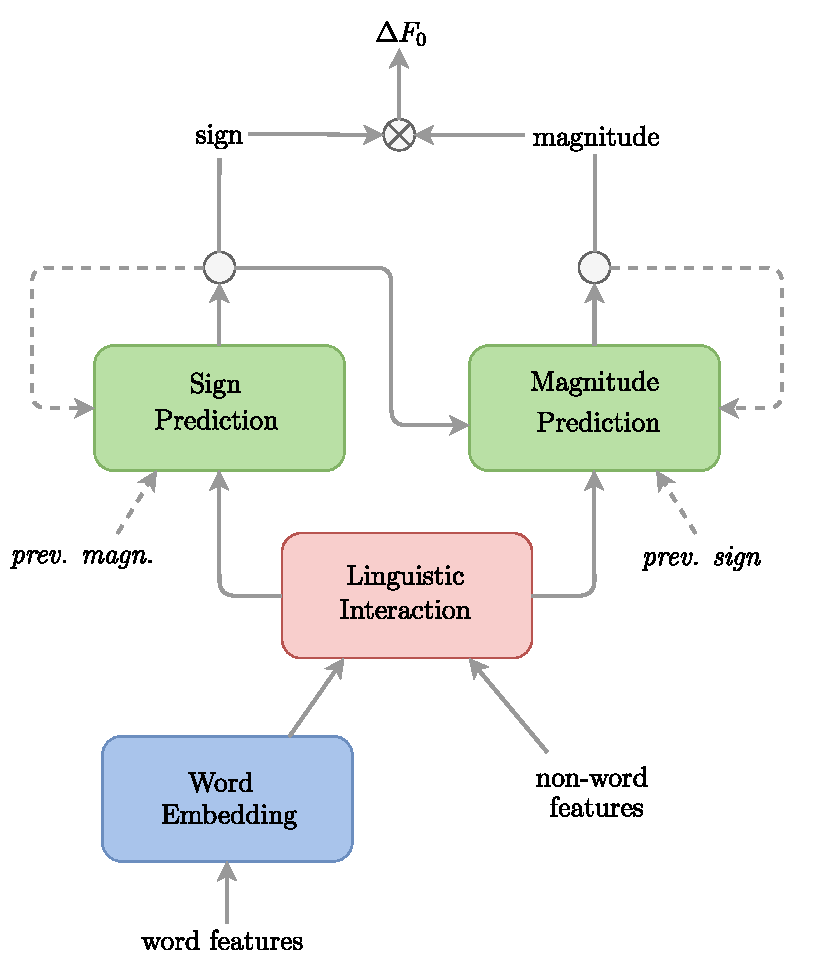
\includegraphics[scale=0.75]{figures/dnn-pipeline.pdf}
    \vspace*{5mm}
    \caption[Intonation model pipeline]{\ac{DNN} pipeline. 
      The dependencies on the previous states are represented by dashed arrows, and the forward dependencies, by plain arrows.
      The blue box corresponds to a \acs{FFNN},
      the red box, to a network composed by a feed-forward layer and a bidirectional recurrent layer, and
      the green box, to a network composed of a feed-forward layer and a forward recurrent layer.}
    \label{fig:dnn-pipeline}
\end{figure}


The word embedding \citep{Levy2014Neural} component is comprised of three  feed-forward layers of the following sizes: 2048, 1024, 512.
The main function of this component is to convert the one-hot word vectors into smaller, denser vectors by projecting the lemma information into a dedicated reduced space.

The next component is the linguistic interaction component.
At this stage, the output of the word embedding component is concatenated with all the other linguistic inputs and passed through one feed-forward layer of size 512.

The purpose of this feed-forward layer is to merge the dense lemma representations and the other linguistic inputs.
This gives inputs a chance to have some local interaction before they are fed to additional layers.

Once the inputs have been processed locally, i.e., within the time step they were emitted, they are fed to pair of \ac{BRNN} layers with 512 \ac{GRU} neurons each.
The purpose of the bidirectional layers is to capture contextual interaction through time.

The last component is composed of two similar sub-components.
These are tasked with the prediction of the sign and magnitude of the dynamic of the \ac{F0}, respectively.
Each sub-component is composed of a simple feed-forward layer of 512 nodes and a forward recurrent layer of 256 \ac{GRU} neurons, to take the context into account.

The input to this last component is the backward and forward states produced by the previous component, plus its own recurrent sign and magnitude states.
In order to align the sign and the magnitude predictions, the magnitude sub-component has additional input coming from the output of the sign sub-component.
ELU \citep{Clevert2015Fast} is used as the activation function for all neurons in the model.






\section{Architectural Details}



\subsection{Word embedding}


In the proposed approach, the training of the word vectors is integrated with the rest of the linguistic features within a single common structure.
The reason behind this choice is that neural networks can model very subtle interactions and detect very fine-grained correlations.
By training word vectors separately, the network cannot guide the dimensionality reduction on the basis of the interactions that these dense word vectors will have downstream with other inputs.
By training all the labels within the same instance, all the interactions between linguistic labels and output labels are allowed to flow back into the feed-forward word layers.

However, because of the size of the word inputs, integrating the training of word embeddings within a common structure can cause significant performance degradation at inference time.
To overcome this, word vectors are given a number of dedicated feed-forward layers, to project the large input vectors into smaller dense vectors.
After the network has been trained, the dense word vectors can be extracted by feeding the one-hot word vectors one after the other.
For each word we can then push the input thought network right until the last feed-forward word layer of the word embedding component.
This last forward layer can be saved and used during inference in lieu of the original one-hot word vectors, thus bypassing the computationally expensive word embedding component.


\subsection{Linguistic interaction}

The linguistic interaction component is tasked with modeling both the local interaction between word and non-word features, but also contextual interactions across multiple time steps.
In the proposed approach, these temporal interactions are modeled by means of \ac{BRNN} layers.
However, this is not the only possible approach, as these could also be modeled with feed-forward layers. 

\acp{FFNN} have successfully been used in \citet{Vainio2001Artificial} to model time series in the context of intonation modeling. 
In their work, the use of feed-forward layers is appropriate, as the author explains that their intention is not to model trajectories or curves directly, but rather instantaneous values within an utterance.

Under their approach, contours are not treated as events that unfold through time, but rather as something more akin to ``static pictures'', where trajectories are just a side-effect of correctly predicting the static values.
The task of the network would then be to match snippets of linguistic inputs to snippets of contour ``pictures''.
Given their initial assumptions and the way their work was set up, it makes sense to use feed-forward layers.\footnote{or even convolutional layers, I would venture to suggest.}

However, within the proposed methodology, this approach does not seem to be appropriate, as the proposed \ac{DNN} is based on a completely different set of assumptions, most of which are antithetical to those underlying their work.
In particular, the main assumption underlying my proposal is that contours are not to be viewed as sequences of ``static pictures'' that we try to fit together in a sequence, but rather as sequences of instructions of interpretable prosodic commands.

Even though \acp{FFNN} can in principle learn time series by using a sliding window, a more common and elegant way to approach tasks involving time series or forecasting is to use \acp{RNN}.
\acp{RNN} are especially suitable for the modeling of time series, as they can be fed arbitrarily long sequences of data, whereas \acp{FFNN} can only model fixed size windows.
Once the size of the window has been decided, we cannot feed inputs whose size is larger than that of the window.
Similarly, inputs of smaller sizes either need to concatenated with other inputs to fill up the input window, or they need to be padded.
Given these limitations associated with \acp{FFNN}, in the proposed model, interactions over time are modeled by means of recurrent layers.

As \acp{RNN} comes in different flavors, it is important to select the most suitable architecture for the task at hand.
Vanilla \acp{RNN} are not optimal for my task, because they can only read the inputs one after the other, with the result that our context is limited to only past observations. 

Even though humans almost never read the entire sentence before reading it out loud, they typically do look ahead and make use of many direct and indirect clues that the network has no access to. 
For instance, humans can extrapolate a lot of information about the general length and structure of a sentence or a paragraph by noticing punctuation symbols, line breaks, etc. 
For all these reasons, it would be desirable to present the neural network with both past and future inputs. 

This can be achieved using \acp{BRNN}, where one recurrent layer reads the input forwards and the other backwards. 
Additionally, \citet{Schuster1997Bidirectional} have shown that \acp{BRNN} achieve better performance than vanilla unidirectional \acp{RNN}.


\subsection{Feed-back Connections}

The last component of the the proposed \ac{DNN} architecture is characterized by a rather complex structure, with multiple inputs and recurrent feed-back connections feeding into it.

This is in contrast with many other approaches, where the output of \acp{BRNN} is fed directly to the output layer to produce a prediction.
This approach would be more than sufficient if we were in the situation in which the input features can only map to one possible output sequence. 
However, in many sequence-to-sequence problems this is often not the case.
Consider for instance the case of \ac{MT}: for every sentence in the source language there are potentially multiple ways in which it can be rendered in the target language.

In this scenario, the task of the neural network is twofold: on the one hand, it has to predict an output sequence that would be fitting for the input sequence; on the other, it has to make sure that each possible rendition of the input sequence is cohesive and coherent within itself.
This means that in the event in which for some input sequence there are two possible output sequences that the network could predict and these two sequences are just as likely, we want the neural network to commit to one and only one of the two possibilities and not to blend different elements from the two that might not coherently fit together.

In \ac{MT}, this problem is often solved by means of feedback and attention mechanisms \citep{Cho2014Learning, Luong2015Effective}. 
Attention mechanisms make sure the network learns to which parts of the inputs it should attend at every step of the prediction.
This is especially important when the inputs are temporally not aligned with the outputs (e.g., when translating from English to German, the verb sometimes has to move to the end of the sentence).

In our particular case, an attention mechanism is not necessary, because our inputs and outputs are already aligned along the time domain.
So, to make sure predictions were coherent, feedback connections from previous outputs are sent into current processing layers. 
This technique has also been used in the context of \ac{MT} to ensure local fluency \citep{Cho2014Learning}.

The introduction of feedback connections is also justified by evidence about the importance of feedback in speech \citep{Borden1980Use}.
Particularly in what concerns intonation, it has been observed that, in postlingually deafened adults, intonation patterns undergo a progressive process of deterioration when feedback weakens as a consequence of hearing loss \citep{Lane1991Speech}.
Alterations in pitch pattern production are also observed in adults with unimpaired hearing in response to manipulated pitch feedback \citep{Burnett1998Voice}.
Adding feedback mechanisms to our network serves as a way to simulate the ability that humans have to hear and utilize their own previous pitch patterns in the generation of subsequent ones.

In order to model sign and magnitude simultaneously, both predictions are integrated within a single shared task.
In \ac{ML}, this technique is commonly referred to as \ac{MTL}.
Aside from the ability to share tasks, there are many additional advantages in using \ac{MTL}: it promotes selection of representations that are useful for all tasks, it allows for transfer learning, it can help focus attention on features that are most relevant, and it provides strong regularization \citep{Ruder2017overview}.

In order to add this sharing-task feature to my network, I first added two parallel feed-forward layers (i.e., the output of one feed-forward layer does not feed into the other), one for the sign and one for the magnitude, where each has its own set of parameters.
Each of the two feed-forward layers takes as input the concatenated current forward and backward states from the bidirectional layers, plus the sign and magnitude outputs predicted at the previous time step.
Then, in order to model sign and magnitude interactions across time, I added one recurrent layer for the sign and one for the magnitude.
Just like the feed-forward layers on top of which they sit, these two recurrent layers run alongside each other, and each has its own set of parameters.
One of these recurrent layers makes predictions for the sign, and the other, for the magnitude.

At each time step the layers involved in the prediction of the sign receive information about the sign and magnitude that have been emitted in the previous time step.
Likewise, the layers involved in the prediction of the magnitude also receive information about the sign and magnitude that have been predicted.
This makes sure that the two sets of layers involved in each task can realign themselves to the other at each time step.

However, even with feedback connections that allow for realignment, we might still have problems of inconsistency within each time step.
This is because the layers involved with the prediction of, say, the magnitude receive only information about what sign and magnitude have been emitted in the previous step, but they do not have access to what the current sign prediction is.
To reduce the chance of inconsistencies within each time step, a connection between the current sign prediction and the current magnitude forward layer has been added.
Under this approach, we assume that the task of sign prediction takes precedence over the task of magnitude prediction.
The idea is that we first decide in which direction we want to move and then we can decide exactly the amount by which we move into that direction.

One important implementation detail is that, during the back-propagation stage, we must not propagate the magnitude error through its connection to the current sign prediction.
If we neglect to take this crucial step, the error from the magnitude will flow into the layers dedicated to the prediction of the sign, which can cause the magnitude error signal to completely take over the sign representations so that they become predictive of the magnitude.
Not only would this defeat the whole purpose of dividing the network into two tasks, but, in my experience, it can often lead to gradient-related errors.

In conclusion, at each time step, the prediction of the sign is conditioned on all the previous, current, and subsequent linguistic inputs, as well as the previous sign and magnitude predictions.
The prediction of the magnitude, on the other hand, is conditioned on all the previous, current, and subsequent linguistic inputs, as well as the previous sign and magnitude predictions, as well as the sign predicted at the current time step.
The predictions that the network emits for both the sign and the magnitude will be used together with the output vectors that we feed to the network as to compute an error function describing the distance between our prediction and the training data.



\subsection{The Error Function}


There are two main error functions that are very popular in the context of deep learning: one is the \ac{RMSE} and the other is the cross-entropy error.

As my problem is not formulated as a classification task, the cross-entropy error function is used.
Even though it is theoretically possible to perform classification using the \ac{RMSE} error function, it has been found that the cross-entropy function leads to faster training and better generalization in classification tasks \citep{Golik2013Cross, Simard2003Best}.



\subsection{The Optimizer}

In contrast with recent and popular trends of using adaptive per-parameter learning methods such as Adagrad \citep{Duchi2011Adaptive}, Adadelta \citep{Zeiler2012ADADELTA}, Rmsprop \citep{Dauphin2015Equilibrated}, Adam \citep{Kingma2014Adam} and Nadam \citep{Dozat2016Incorporating}, I decided to adopt a variant of the classical \ac{SGD} algorithm.

Recently, it has been found that, for over-parametrized problems, as it is the case for most current deep learning applications, adaptive optimization methods can produce drastically different solutions, as well as models that generalize significantly worse than \ac{SGD}, even when they perform better on the training data \citep{Wilson2017Marginal}.
This observation was also at the basis of one of the recommendations offered by \citet{Hoffer2017Train} on how to train models that can generalize better.

For these reasons, in my implementation I used \ac{SGD} with Nesterov Momentum, also called \ac{NAG}, which is a faster variant of Momentum optimization \citep{Nesterov1983method}.


\section{Accuracy Issues}

One issue that is particularly hard to address in intonation modeling is how to measure accuracy during the training phase and what stopping criterion should be used.

When intonation is treated as a regression problem, i.e., when using log(\ac{F0}) as input and \ac{RMSE} error as the error function, the obvious solution would be to simply use the loss on the function as a measure of accuracy.
By calculating the loss on both the training and the validation set we can stop training as soon as the loss on the validation set starts increasing.
This is a commonly employed technique also known as early-stopping.

The problem is that intonation is a highly unpredictable phenomenon.
For every sentence, multiple completely different, yet plausible, renditions are possible.
Which one of these should be predicted is highly dependent on a number of contingent factors (e.g., linguistic context, the speaker's psychological state,  the addressee, etc.), many of which are not available to the network. 
This means that at some point of the training process, we might produce contours that sound natural because they capture general prosodic properties from the corpus very well.
However, the loss from these contours might be very high because the reference sentences just happen to be a completely different and equally plausible rendition of the input.
A consequence of this possibility is that we cannot heavily rely on the loss of the neural network to measure the progress on the training.


As we currently do not have a reliable method to automatically measure the appropriateness of a specific contour against a specific set of linguistic inputs, the strategy adopted in my methodology was to save a copy of the model at the end of each epoch.
After training, I selected one by listening to the synthetic contours it generated for the validation set.



\section{Overfitting Issues}

The reason why it is so important to determine the most appropriate time to stop the training of the network is because models produced at different epochs will be radically different.

If we train the model for too long, we start capturing too many details about the training data, many of which are specific to the training set and will not generalize well for new observations.
This phenomenon is due to fitting the training data too closely and in machine learning it is also known and overfitting.

The chance of overfitting is particularly high in my model, because of the high number of parameters and the inclusion of very large layers for word vectors.
One commonly used technique to alleviate this problem, is dropout.
With dropout, the contributions of a subset of the neurons during training \citep{Srivastava2014Dropout} are temporarily and randomly excluded.
This process introduces noise and temporarily prevents some of the inputs from reaching all the nodes in the network, thus reducing the chance that complex co-adaptations might emerge and forcing the network to make predictions only from partial sources of information.
Despite its simplicity, dropout is very effective at reducing overfitting and is one of the most common regularizing techniques used in deep learning.

Because of these reasons, I added dropout to all the feed-forward layers of the network.
This substantially alleviated the overfitting problem, which resulted in more consistent models across training epochs.

In previous sections, feed-forward layers preceding recurrent layers were justified as locations in the network to allow for local interactions between inputs.
In addition to this main reason, feed-forward layers were also used to provide a convenient location to apply dropout.

In my architecture, there are many locations where one-hot vectors are concatenated with dense vectors before they are processed by recurrent layers.
For instance, non-word linguistic inputs are concatenated with feed-forward layers before they are passed through bidirectional layers.

As we cannot apply dropout to very sparse vectors such as the one-hot vectors (because most of their inputs are already mostly zeros), feed-forward layers provide for a convenient location where we can merge sparse inputs with dense inputs to create a single dense representation, onto which dropout can be applied.

\section{Data augmentation}

Even though dropout produced a substantial improvement in the quality of the synthetic contours and greatly increased consistency across models, many of the predicted contours still contained extreme and implausible pitch excursions or pitch drops.

My hypothesis for this behavior was that the network was suffering from the so-called \textit{exposure bias} problem.
Exposure bias refers to a phenomenon often observed in generative models where outputs are fed back and used as inputs for subsequent output generation.

As explained by \citet{Ranzato2015Sequence}, the problem is that during training, the model only utilizes the gold-standard output as its feedback and not its own predictions, which at inference time are bound to contain some errors or deviations from the original distribution.
This discrepancy makes prediction brittle, as generation errors may accumulate over time.

One way to solve this issue is to randomly expose the network to either the ground-truth or its own predictions during training.
However, this approach has been argued to be theoretically flawed \citep{Huszar2015How} and not particularly successful in the context of \ac{F0} modeling \citep{Wang2017RNN}, where instead one of the proposed solutions is to use dropout to occasionally remove feedback.
However, in my network I already had dropout applied to the feedback connections and although dropout did help improve performance, it never completely eliminated the problem.

One thing I noticed was that often, the most problematic utterances were also the longest.
On the one hand, this behavior is expected, as it is consistent with the exposure bias hypothesis: longer utterances allow for a larger margin of error, as we have more steps to predict and therefore more opportunities for generating errors.
On the other hand, I could not understand why, once the prediction starts moving in the wrong direction, the network is unable to detect it and correct it.

It is easy to understand why generation errors are very problematic in language modeling, where interactions between words may have very unpredictable effects and errors are very hard to recover from.
In humans, recovering strategies from these kind of errors is anything but trivial, as it often involves cognitively challenging tasks such as detecting the problem in the first place, rephrasing the problematic segment, or finding a convoluted and yet graceful way of still completing the utterance.
These are all tasks that most neural networks are not trained to perform.

In our case, the property that we want to capture, and that is required to avoid getting out of a certain range, is a lot coarser and easier to define.
This property is very apparent when we observe the \ac{F0} contour over very long stretches of speech such as in \autoref{fig:pseudo-periodicity}: pseudo-periodicity.

\begin{figure}[h]
\centering
\resizebox{\textwidth}{!}{%% Creator: Matplotlib, PGF backend
%%
%% To include the figure in your LaTeX document, write
%%   \input{<filename>.pgf}
%%
%% Make sure the required packages are loaded in your preamble
%%   \usepackage{pgf}
%%
%% Figures using additional raster images can only be included by \input if
%% they are in the same directory as the main LaTeX file. For loading figures
%% from other directories you can use the `import` package
%%   \usepackage{import}
%% and then include the figures with
%%   \import{<path to file>}{<filename>.pgf}
%%
%% Matplotlib used the following preamble
%%   \usepackage[utf8x]{inputenc}
%%   \usepackage[T1]{fontenc}
%%   \usepackage{cmbright}
%%
\begingroup%
\makeatletter%
\begin{pgfpicture}%
\pgfpathrectangle{\pgfpointorigin}{\pgfqpoint{8.000000in}{4.000000in}}%
\pgfusepath{use as bounding box, clip}%
\begin{pgfscope}%
\pgfsetbuttcap%
\pgfsetmiterjoin%
\definecolor{currentfill}{rgb}{1.000000,1.000000,1.000000}%
\pgfsetfillcolor{currentfill}%
\pgfsetlinewidth{0.000000pt}%
\definecolor{currentstroke}{rgb}{1.000000,1.000000,1.000000}%
\pgfsetstrokecolor{currentstroke}%
\pgfsetdash{}{0pt}%
\pgfpathmoveto{\pgfqpoint{0.000000in}{0.000000in}}%
\pgfpathlineto{\pgfqpoint{8.000000in}{0.000000in}}%
\pgfpathlineto{\pgfqpoint{8.000000in}{4.000000in}}%
\pgfpathlineto{\pgfqpoint{0.000000in}{4.000000in}}%
\pgfpathclose%
\pgfusepath{fill}%
\end{pgfscope}%
\begin{pgfscope}%
\pgfsetbuttcap%
\pgfsetmiterjoin%
\definecolor{currentfill}{rgb}{1.000000,1.000000,1.000000}%
\pgfsetfillcolor{currentfill}%
\pgfsetlinewidth{0.000000pt}%
\definecolor{currentstroke}{rgb}{0.000000,0.000000,0.000000}%
\pgfsetstrokecolor{currentstroke}%
\pgfsetstrokeopacity{0.000000}%
\pgfsetdash{}{0pt}%
\pgfpathmoveto{\pgfqpoint{1.000000in}{0.440000in}}%
\pgfpathlineto{\pgfqpoint{7.200000in}{0.440000in}}%
\pgfpathlineto{\pgfqpoint{7.200000in}{3.520000in}}%
\pgfpathlineto{\pgfqpoint{1.000000in}{3.520000in}}%
\pgfpathclose%
\pgfusepath{fill}%
\end{pgfscope}%
\begin{pgfscope}%
\pgfsetbuttcap%
\pgfsetroundjoin%
\definecolor{currentfill}{rgb}{0.000000,0.000000,0.000000}%
\pgfsetfillcolor{currentfill}%
\pgfsetlinewidth{0.803000pt}%
\definecolor{currentstroke}{rgb}{0.000000,0.000000,0.000000}%
\pgfsetstrokecolor{currentstroke}%
\pgfsetdash{}{0pt}%
\pgfsys@defobject{currentmarker}{\pgfqpoint{0.000000in}{-0.048611in}}{\pgfqpoint{0.000000in}{0.000000in}}{%
\pgfpathmoveto{\pgfqpoint{0.000000in}{0.000000in}}%
\pgfpathlineto{\pgfqpoint{0.000000in}{-0.048611in}}%
\pgfusepath{stroke,fill}%
}%
\begin{pgfscope}%
\pgfsys@transformshift{1.281818in}{0.440000in}%
\pgfsys@useobject{currentmarker}{}%
\end{pgfscope}%
\end{pgfscope}%
\begin{pgfscope}%
\pgftext[x=1.281818in,y=0.342778in,,top]{\rmfamily\fontsize{10.000000}{12.000000}\selectfont \(\displaystyle 0\)}%
\end{pgfscope}%
\begin{pgfscope}%
\pgfsetbuttcap%
\pgfsetroundjoin%
\definecolor{currentfill}{rgb}{0.000000,0.000000,0.000000}%
\pgfsetfillcolor{currentfill}%
\pgfsetlinewidth{0.803000pt}%
\definecolor{currentstroke}{rgb}{0.000000,0.000000,0.000000}%
\pgfsetstrokecolor{currentstroke}%
\pgfsetdash{}{0pt}%
\pgfsys@defobject{currentmarker}{\pgfqpoint{0.000000in}{-0.048611in}}{\pgfqpoint{0.000000in}{0.000000in}}{%
\pgfpathmoveto{\pgfqpoint{0.000000in}{0.000000in}}%
\pgfpathlineto{\pgfqpoint{0.000000in}{-0.048611in}}%
\pgfusepath{stroke,fill}%
}%
\begin{pgfscope}%
\pgfsys@transformshift{2.226249in}{0.440000in}%
\pgfsys@useobject{currentmarker}{}%
\end{pgfscope}%
\end{pgfscope}%
\begin{pgfscope}%
\pgftext[x=2.226249in,y=0.342778in,,top]{\rmfamily\fontsize{10.000000}{12.000000}\selectfont \(\displaystyle 5\)}%
\end{pgfscope}%
\begin{pgfscope}%
\pgfsetbuttcap%
\pgfsetroundjoin%
\definecolor{currentfill}{rgb}{0.000000,0.000000,0.000000}%
\pgfsetfillcolor{currentfill}%
\pgfsetlinewidth{0.803000pt}%
\definecolor{currentstroke}{rgb}{0.000000,0.000000,0.000000}%
\pgfsetstrokecolor{currentstroke}%
\pgfsetdash{}{0pt}%
\pgfsys@defobject{currentmarker}{\pgfqpoint{0.000000in}{-0.048611in}}{\pgfqpoint{0.000000in}{0.000000in}}{%
\pgfpathmoveto{\pgfqpoint{0.000000in}{0.000000in}}%
\pgfpathlineto{\pgfqpoint{0.000000in}{-0.048611in}}%
\pgfusepath{stroke,fill}%
}%
\begin{pgfscope}%
\pgfsys@transformshift{3.170680in}{0.440000in}%
\pgfsys@useobject{currentmarker}{}%
\end{pgfscope}%
\end{pgfscope}%
\begin{pgfscope}%
\pgftext[x=3.170680in,y=0.342778in,,top]{\rmfamily\fontsize{10.000000}{12.000000}\selectfont \(\displaystyle 10\)}%
\end{pgfscope}%
\begin{pgfscope}%
\pgfsetbuttcap%
\pgfsetroundjoin%
\definecolor{currentfill}{rgb}{0.000000,0.000000,0.000000}%
\pgfsetfillcolor{currentfill}%
\pgfsetlinewidth{0.803000pt}%
\definecolor{currentstroke}{rgb}{0.000000,0.000000,0.000000}%
\pgfsetstrokecolor{currentstroke}%
\pgfsetdash{}{0pt}%
\pgfsys@defobject{currentmarker}{\pgfqpoint{0.000000in}{-0.048611in}}{\pgfqpoint{0.000000in}{0.000000in}}{%
\pgfpathmoveto{\pgfqpoint{0.000000in}{0.000000in}}%
\pgfpathlineto{\pgfqpoint{0.000000in}{-0.048611in}}%
\pgfusepath{stroke,fill}%
}%
\begin{pgfscope}%
\pgfsys@transformshift{4.115111in}{0.440000in}%
\pgfsys@useobject{currentmarker}{}%
\end{pgfscope}%
\end{pgfscope}%
\begin{pgfscope}%
\pgftext[x=4.115111in,y=0.342778in,,top]{\rmfamily\fontsize{10.000000}{12.000000}\selectfont \(\displaystyle 15\)}%
\end{pgfscope}%
\begin{pgfscope}%
\pgfsetbuttcap%
\pgfsetroundjoin%
\definecolor{currentfill}{rgb}{0.000000,0.000000,0.000000}%
\pgfsetfillcolor{currentfill}%
\pgfsetlinewidth{0.803000pt}%
\definecolor{currentstroke}{rgb}{0.000000,0.000000,0.000000}%
\pgfsetstrokecolor{currentstroke}%
\pgfsetdash{}{0pt}%
\pgfsys@defobject{currentmarker}{\pgfqpoint{0.000000in}{-0.048611in}}{\pgfqpoint{0.000000in}{0.000000in}}{%
\pgfpathmoveto{\pgfqpoint{0.000000in}{0.000000in}}%
\pgfpathlineto{\pgfqpoint{0.000000in}{-0.048611in}}%
\pgfusepath{stroke,fill}%
}%
\begin{pgfscope}%
\pgfsys@transformshift{5.059542in}{0.440000in}%
\pgfsys@useobject{currentmarker}{}%
\end{pgfscope}%
\end{pgfscope}%
\begin{pgfscope}%
\pgftext[x=5.059542in,y=0.342778in,,top]{\rmfamily\fontsize{10.000000}{12.000000}\selectfont \(\displaystyle 20\)}%
\end{pgfscope}%
\begin{pgfscope}%
\pgfsetbuttcap%
\pgfsetroundjoin%
\definecolor{currentfill}{rgb}{0.000000,0.000000,0.000000}%
\pgfsetfillcolor{currentfill}%
\pgfsetlinewidth{0.803000pt}%
\definecolor{currentstroke}{rgb}{0.000000,0.000000,0.000000}%
\pgfsetstrokecolor{currentstroke}%
\pgfsetdash{}{0pt}%
\pgfsys@defobject{currentmarker}{\pgfqpoint{0.000000in}{-0.048611in}}{\pgfqpoint{0.000000in}{0.000000in}}{%
\pgfpathmoveto{\pgfqpoint{0.000000in}{0.000000in}}%
\pgfpathlineto{\pgfqpoint{0.000000in}{-0.048611in}}%
\pgfusepath{stroke,fill}%
}%
\begin{pgfscope}%
\pgfsys@transformshift{6.003973in}{0.440000in}%
\pgfsys@useobject{currentmarker}{}%
\end{pgfscope}%
\end{pgfscope}%
\begin{pgfscope}%
\pgftext[x=6.003973in,y=0.342778in,,top]{\rmfamily\fontsize{10.000000}{12.000000}\selectfont \(\displaystyle 25\)}%
\end{pgfscope}%
\begin{pgfscope}%
\pgfsetbuttcap%
\pgfsetroundjoin%
\definecolor{currentfill}{rgb}{0.000000,0.000000,0.000000}%
\pgfsetfillcolor{currentfill}%
\pgfsetlinewidth{0.803000pt}%
\definecolor{currentstroke}{rgb}{0.000000,0.000000,0.000000}%
\pgfsetstrokecolor{currentstroke}%
\pgfsetdash{}{0pt}%
\pgfsys@defobject{currentmarker}{\pgfqpoint{0.000000in}{-0.048611in}}{\pgfqpoint{0.000000in}{0.000000in}}{%
\pgfpathmoveto{\pgfqpoint{0.000000in}{0.000000in}}%
\pgfpathlineto{\pgfqpoint{0.000000in}{-0.048611in}}%
\pgfusepath{stroke,fill}%
}%
\begin{pgfscope}%
\pgfsys@transformshift{6.948404in}{0.440000in}%
\pgfsys@useobject{currentmarker}{}%
\end{pgfscope}%
\end{pgfscope}%
\begin{pgfscope}%
\pgftext[x=6.948404in,y=0.342778in,,top]{\rmfamily\fontsize{10.000000}{12.000000}\selectfont \(\displaystyle 30\)}%
\end{pgfscope}%
\begin{pgfscope}%
\pgftext[x=4.100000in,y=0.164567in,,top]{\rmfamily\fontsize{10.000000}{12.000000}\selectfont Time (s)}%
\end{pgfscope}%
\begin{pgfscope}%
\pgfsetbuttcap%
\pgfsetroundjoin%
\definecolor{currentfill}{rgb}{0.000000,0.000000,0.000000}%
\pgfsetfillcolor{currentfill}%
\pgfsetlinewidth{0.803000pt}%
\definecolor{currentstroke}{rgb}{0.000000,0.000000,0.000000}%
\pgfsetstrokecolor{currentstroke}%
\pgfsetdash{}{0pt}%
\pgfsys@defobject{currentmarker}{\pgfqpoint{-0.048611in}{0.000000in}}{\pgfqpoint{0.000000in}{0.000000in}}{%
\pgfpathmoveto{\pgfqpoint{0.000000in}{0.000000in}}%
\pgfpathlineto{\pgfqpoint{-0.048611in}{0.000000in}}%
\pgfusepath{stroke,fill}%
}%
\begin{pgfscope}%
\pgfsys@transformshift{1.000000in}{0.547381in}%
\pgfsys@useobject{currentmarker}{}%
\end{pgfscope}%
\end{pgfscope}%
\begin{pgfscope}%
\pgftext[x=0.684030in,y=0.499553in,left,base]{\rmfamily\fontsize{10.000000}{12.000000}\selectfont \(\displaystyle 125\)}%
\end{pgfscope}%
\begin{pgfscope}%
\pgfsetbuttcap%
\pgfsetroundjoin%
\definecolor{currentfill}{rgb}{0.000000,0.000000,0.000000}%
\pgfsetfillcolor{currentfill}%
\pgfsetlinewidth{0.803000pt}%
\definecolor{currentstroke}{rgb}{0.000000,0.000000,0.000000}%
\pgfsetstrokecolor{currentstroke}%
\pgfsetdash{}{0pt}%
\pgfsys@defobject{currentmarker}{\pgfqpoint{-0.048611in}{0.000000in}}{\pgfqpoint{0.000000in}{0.000000in}}{%
\pgfpathmoveto{\pgfqpoint{0.000000in}{0.000000in}}%
\pgfpathlineto{\pgfqpoint{-0.048611in}{0.000000in}}%
\pgfusepath{stroke,fill}%
}%
\begin{pgfscope}%
\pgfsys@transformshift{1.000000in}{0.952543in}%
\pgfsys@useobject{currentmarker}{}%
\end{pgfscope}%
\end{pgfscope}%
\begin{pgfscope}%
\pgftext[x=0.684030in,y=0.904715in,left,base]{\rmfamily\fontsize{10.000000}{12.000000}\selectfont \(\displaystyle 150\)}%
\end{pgfscope}%
\begin{pgfscope}%
\pgfsetbuttcap%
\pgfsetroundjoin%
\definecolor{currentfill}{rgb}{0.000000,0.000000,0.000000}%
\pgfsetfillcolor{currentfill}%
\pgfsetlinewidth{0.803000pt}%
\definecolor{currentstroke}{rgb}{0.000000,0.000000,0.000000}%
\pgfsetstrokecolor{currentstroke}%
\pgfsetdash{}{0pt}%
\pgfsys@defobject{currentmarker}{\pgfqpoint{-0.048611in}{0.000000in}}{\pgfqpoint{0.000000in}{0.000000in}}{%
\pgfpathmoveto{\pgfqpoint{0.000000in}{0.000000in}}%
\pgfpathlineto{\pgfqpoint{-0.048611in}{0.000000in}}%
\pgfusepath{stroke,fill}%
}%
\begin{pgfscope}%
\pgfsys@transformshift{1.000000in}{1.357705in}%
\pgfsys@useobject{currentmarker}{}%
\end{pgfscope}%
\end{pgfscope}%
\begin{pgfscope}%
\pgftext[x=0.684030in,y=1.309877in,left,base]{\rmfamily\fontsize{10.000000}{12.000000}\selectfont \(\displaystyle 175\)}%
\end{pgfscope}%
\begin{pgfscope}%
\pgfsetbuttcap%
\pgfsetroundjoin%
\definecolor{currentfill}{rgb}{0.000000,0.000000,0.000000}%
\pgfsetfillcolor{currentfill}%
\pgfsetlinewidth{0.803000pt}%
\definecolor{currentstroke}{rgb}{0.000000,0.000000,0.000000}%
\pgfsetstrokecolor{currentstroke}%
\pgfsetdash{}{0pt}%
\pgfsys@defobject{currentmarker}{\pgfqpoint{-0.048611in}{0.000000in}}{\pgfqpoint{0.000000in}{0.000000in}}{%
\pgfpathmoveto{\pgfqpoint{0.000000in}{0.000000in}}%
\pgfpathlineto{\pgfqpoint{-0.048611in}{0.000000in}}%
\pgfusepath{stroke,fill}%
}%
\begin{pgfscope}%
\pgfsys@transformshift{1.000000in}{1.762867in}%
\pgfsys@useobject{currentmarker}{}%
\end{pgfscope}%
\end{pgfscope}%
\begin{pgfscope}%
\pgftext[x=0.684030in,y=1.715040in,left,base]{\rmfamily\fontsize{10.000000}{12.000000}\selectfont \(\displaystyle 200\)}%
\end{pgfscope}%
\begin{pgfscope}%
\pgfsetbuttcap%
\pgfsetroundjoin%
\definecolor{currentfill}{rgb}{0.000000,0.000000,0.000000}%
\pgfsetfillcolor{currentfill}%
\pgfsetlinewidth{0.803000pt}%
\definecolor{currentstroke}{rgb}{0.000000,0.000000,0.000000}%
\pgfsetstrokecolor{currentstroke}%
\pgfsetdash{}{0pt}%
\pgfsys@defobject{currentmarker}{\pgfqpoint{-0.048611in}{0.000000in}}{\pgfqpoint{0.000000in}{0.000000in}}{%
\pgfpathmoveto{\pgfqpoint{0.000000in}{0.000000in}}%
\pgfpathlineto{\pgfqpoint{-0.048611in}{0.000000in}}%
\pgfusepath{stroke,fill}%
}%
\begin{pgfscope}%
\pgfsys@transformshift{1.000000in}{2.168029in}%
\pgfsys@useobject{currentmarker}{}%
\end{pgfscope}%
\end{pgfscope}%
\begin{pgfscope}%
\pgftext[x=0.684030in,y=2.120202in,left,base]{\rmfamily\fontsize{10.000000}{12.000000}\selectfont \(\displaystyle 225\)}%
\end{pgfscope}%
\begin{pgfscope}%
\pgfsetbuttcap%
\pgfsetroundjoin%
\definecolor{currentfill}{rgb}{0.000000,0.000000,0.000000}%
\pgfsetfillcolor{currentfill}%
\pgfsetlinewidth{0.803000pt}%
\definecolor{currentstroke}{rgb}{0.000000,0.000000,0.000000}%
\pgfsetstrokecolor{currentstroke}%
\pgfsetdash{}{0pt}%
\pgfsys@defobject{currentmarker}{\pgfqpoint{-0.048611in}{0.000000in}}{\pgfqpoint{0.000000in}{0.000000in}}{%
\pgfpathmoveto{\pgfqpoint{0.000000in}{0.000000in}}%
\pgfpathlineto{\pgfqpoint{-0.048611in}{0.000000in}}%
\pgfusepath{stroke,fill}%
}%
\begin{pgfscope}%
\pgfsys@transformshift{1.000000in}{2.573192in}%
\pgfsys@useobject{currentmarker}{}%
\end{pgfscope}%
\end{pgfscope}%
\begin{pgfscope}%
\pgftext[x=0.684030in,y=2.525364in,left,base]{\rmfamily\fontsize{10.000000}{12.000000}\selectfont \(\displaystyle 250\)}%
\end{pgfscope}%
\begin{pgfscope}%
\pgfsetbuttcap%
\pgfsetroundjoin%
\definecolor{currentfill}{rgb}{0.000000,0.000000,0.000000}%
\pgfsetfillcolor{currentfill}%
\pgfsetlinewidth{0.803000pt}%
\definecolor{currentstroke}{rgb}{0.000000,0.000000,0.000000}%
\pgfsetstrokecolor{currentstroke}%
\pgfsetdash{}{0pt}%
\pgfsys@defobject{currentmarker}{\pgfqpoint{-0.048611in}{0.000000in}}{\pgfqpoint{0.000000in}{0.000000in}}{%
\pgfpathmoveto{\pgfqpoint{0.000000in}{0.000000in}}%
\pgfpathlineto{\pgfqpoint{-0.048611in}{0.000000in}}%
\pgfusepath{stroke,fill}%
}%
\begin{pgfscope}%
\pgfsys@transformshift{1.000000in}{2.978354in}%
\pgfsys@useobject{currentmarker}{}%
\end{pgfscope}%
\end{pgfscope}%
\begin{pgfscope}%
\pgftext[x=0.684030in,y=2.930526in,left,base]{\rmfamily\fontsize{10.000000}{12.000000}\selectfont \(\displaystyle 275\)}%
\end{pgfscope}%
\begin{pgfscope}%
\pgfsetbuttcap%
\pgfsetroundjoin%
\definecolor{currentfill}{rgb}{0.000000,0.000000,0.000000}%
\pgfsetfillcolor{currentfill}%
\pgfsetlinewidth{0.803000pt}%
\definecolor{currentstroke}{rgb}{0.000000,0.000000,0.000000}%
\pgfsetstrokecolor{currentstroke}%
\pgfsetdash{}{0pt}%
\pgfsys@defobject{currentmarker}{\pgfqpoint{-0.048611in}{0.000000in}}{\pgfqpoint{0.000000in}{0.000000in}}{%
\pgfpathmoveto{\pgfqpoint{0.000000in}{0.000000in}}%
\pgfpathlineto{\pgfqpoint{-0.048611in}{0.000000in}}%
\pgfusepath{stroke,fill}%
}%
\begin{pgfscope}%
\pgfsys@transformshift{1.000000in}{3.383516in}%
\pgfsys@useobject{currentmarker}{}%
\end{pgfscope}%
\end{pgfscope}%
\begin{pgfscope}%
\pgftext[x=0.684030in,y=3.335688in,left,base]{\rmfamily\fontsize{10.000000}{12.000000}\selectfont \(\displaystyle 300\)}%
\end{pgfscope}%
\begin{pgfscope}%
\pgftext[x=0.628474in,y=1.980000in,,bottom,rotate=90.000000]{\rmfamily\fontsize{10.000000}{12.000000}\selectfont Frequency (Hz)}%
\end{pgfscope}%
\begin{pgfscope}%
\pgfpathrectangle{\pgfqpoint{1.000000in}{0.440000in}}{\pgfqpoint{6.200000in}{3.080000in}} %
\pgfusepath{clip}%
\pgfsetrectcap%
\pgfsetroundjoin%
\pgfsetlinewidth{1.505625pt}%
\definecolor{currentstroke}{rgb}{0.364706,0.517647,0.572549}%
\pgfsetstrokecolor{currentstroke}%
\pgfsetdash{}{0pt}%
\pgfpathmoveto{\pgfqpoint{1.281818in}{1.858291in}}%
\pgfpathlineto{\pgfqpoint{1.384761in}{1.857507in}}%
\pgfpathlineto{\pgfqpoint{1.386650in}{1.855635in}}%
\pgfpathlineto{\pgfqpoint{1.388539in}{1.850690in}}%
\pgfpathlineto{\pgfqpoint{1.390428in}{1.839834in}}%
\pgfpathlineto{\pgfqpoint{1.393261in}{1.806260in}}%
\pgfpathlineto{\pgfqpoint{1.402705in}{1.661893in}}%
\pgfpathlineto{\pgfqpoint{1.403650in}{1.661481in}}%
\pgfpathlineto{\pgfqpoint{1.405539in}{1.668399in}}%
\pgfpathlineto{\pgfqpoint{1.409316in}{1.699475in}}%
\pgfpathlineto{\pgfqpoint{1.422538in}{1.822012in}}%
\pgfpathlineto{\pgfqpoint{1.423483in}{1.821241in}}%
\pgfpathlineto{\pgfqpoint{1.425372in}{1.814341in}}%
\pgfpathlineto{\pgfqpoint{1.429149in}{1.800011in}}%
\pgfpathlineto{\pgfqpoint{1.430094in}{1.801353in}}%
\pgfpathlineto{\pgfqpoint{1.431983in}{1.813936in}}%
\pgfpathlineto{\pgfqpoint{1.434816in}{1.858645in}}%
\pgfpathlineto{\pgfqpoint{1.438594in}{1.963244in}}%
\pgfpathlineto{\pgfqpoint{1.444260in}{2.205088in}}%
\pgfpathlineto{\pgfqpoint{1.451816in}{2.529977in}}%
\pgfpathlineto{\pgfqpoint{1.453705in}{2.558580in}}%
\pgfpathlineto{\pgfqpoint{1.454649in}{2.558774in}}%
\pgfpathlineto{\pgfqpoint{1.456538in}{2.532489in}}%
\pgfpathlineto{\pgfqpoint{1.462204in}{2.418734in}}%
\pgfpathlineto{\pgfqpoint{1.463149in}{2.426437in}}%
\pgfpathlineto{\pgfqpoint{1.465038in}{2.477436in}}%
\pgfpathlineto{\pgfqpoint{1.468816in}{2.677922in}}%
\pgfpathlineto{\pgfqpoint{1.473538in}{2.912222in}}%
\pgfpathlineto{\pgfqpoint{1.476371in}{2.963771in}}%
\pgfpathlineto{\pgfqpoint{1.477315in}{2.965659in}}%
\pgfpathlineto{\pgfqpoint{1.479204in}{2.957068in}}%
\pgfpathlineto{\pgfqpoint{1.481093in}{2.950435in}}%
\pgfpathlineto{\pgfqpoint{1.482038in}{2.954342in}}%
\pgfpathlineto{\pgfqpoint{1.483926in}{2.981813in}}%
\pgfpathlineto{\pgfqpoint{1.488649in}{3.066553in}}%
\pgfpathlineto{\pgfqpoint{1.489593in}{3.061352in}}%
\pgfpathlineto{\pgfqpoint{1.491482in}{3.018564in}}%
\pgfpathlineto{\pgfqpoint{1.495260in}{2.850665in}}%
\pgfpathlineto{\pgfqpoint{1.512259in}{2.047930in}}%
\pgfpathlineto{\pgfqpoint{1.531148in}{1.219009in}}%
\pgfpathlineto{\pgfqpoint{1.534926in}{1.145358in}}%
\pgfpathlineto{\pgfqpoint{1.536815in}{1.134579in}}%
\pgfpathlineto{\pgfqpoint{1.537759in}{1.133937in}}%
\pgfpathlineto{\pgfqpoint{1.539648in}{1.138884in}}%
\pgfpathlineto{\pgfqpoint{1.547203in}{1.169344in}}%
\pgfpathlineto{\pgfqpoint{1.549092in}{1.160096in}}%
\pgfpathlineto{\pgfqpoint{1.550981in}{1.134622in}}%
\pgfpathlineto{\pgfqpoint{1.554759in}{1.034713in}}%
\pgfpathlineto{\pgfqpoint{1.559481in}{0.910967in}}%
\pgfpathlineto{\pgfqpoint{1.561370in}{0.894575in}}%
\pgfpathlineto{\pgfqpoint{1.562314in}{0.894261in}}%
\pgfpathlineto{\pgfqpoint{1.564203in}{0.905120in}}%
\pgfpathlineto{\pgfqpoint{1.593480in}{1.175945in}}%
\pgfpathlineto{\pgfqpoint{1.600091in}{1.218750in}}%
\pgfpathlineto{\pgfqpoint{1.606702in}{1.256126in}}%
\pgfpathlineto{\pgfqpoint{1.611425in}{1.298660in}}%
\pgfpathlineto{\pgfqpoint{1.620869in}{1.396278in}}%
\pgfpathlineto{\pgfqpoint{1.621813in}{1.398301in}}%
\pgfpathlineto{\pgfqpoint{1.622758in}{1.397106in}}%
\pgfpathlineto{\pgfqpoint{1.624647in}{1.384804in}}%
\pgfpathlineto{\pgfqpoint{1.627480in}{1.345858in}}%
\pgfpathlineto{\pgfqpoint{1.634091in}{1.213559in}}%
\pgfpathlineto{\pgfqpoint{1.645424in}{0.957448in}}%
\pgfpathlineto{\pgfqpoint{1.648257in}{0.945575in}}%
\pgfpathlineto{\pgfqpoint{1.650146in}{0.945997in}}%
\pgfpathlineto{\pgfqpoint{1.652035in}{0.947213in}}%
\pgfpathlineto{\pgfqpoint{1.652980in}{0.946582in}}%
\pgfpathlineto{\pgfqpoint{1.654868in}{0.940078in}}%
\pgfpathlineto{\pgfqpoint{1.657702in}{0.912503in}}%
\pgfpathlineto{\pgfqpoint{1.664313in}{0.825630in}}%
\pgfpathlineto{\pgfqpoint{1.666202in}{0.819786in}}%
\pgfpathlineto{\pgfqpoint{1.667146in}{0.820123in}}%
\pgfpathlineto{\pgfqpoint{1.674701in}{0.832314in}}%
\pgfpathlineto{\pgfqpoint{1.677535in}{0.831141in}}%
\pgfpathlineto{\pgfqpoint{1.685090in}{0.824516in}}%
\pgfpathlineto{\pgfqpoint{1.687923in}{0.820116in}}%
\pgfpathlineto{\pgfqpoint{1.690757in}{0.811055in}}%
\pgfpathlineto{\pgfqpoint{1.693590in}{0.793511in}}%
\pgfpathlineto{\pgfqpoint{1.703979in}{0.711281in}}%
\pgfpathlineto{\pgfqpoint{1.704923in}{0.711182in}}%
\pgfpathlineto{\pgfqpoint{1.706812in}{0.717343in}}%
\pgfpathlineto{\pgfqpoint{1.709645in}{0.740302in}}%
\pgfpathlineto{\pgfqpoint{1.722867in}{0.891587in}}%
\pgfpathlineto{\pgfqpoint{1.728534in}{0.983588in}}%
\pgfpathlineto{\pgfqpoint{1.738923in}{1.197105in}}%
\pgfpathlineto{\pgfqpoint{1.741756in}{1.307612in}}%
\pgfpathlineto{\pgfqpoint{1.744589in}{1.537922in}}%
\pgfpathlineto{\pgfqpoint{1.747423in}{1.974020in}}%
\pgfpathlineto{\pgfqpoint{1.753089in}{3.374819in}}%
\pgfpathlineto{\pgfqpoint{1.754034in}{3.320698in}}%
\pgfpathlineto{\pgfqpoint{1.789922in}{1.319723in}}%
\pgfpathlineto{\pgfqpoint{1.793700in}{1.211629in}}%
\pgfpathlineto{\pgfqpoint{1.796533in}{1.174999in}}%
\pgfpathlineto{\pgfqpoint{1.799366in}{1.163430in}}%
\pgfpathlineto{\pgfqpoint{1.801255in}{1.162388in}}%
\pgfpathlineto{\pgfqpoint{1.804088in}{1.163694in}}%
\pgfpathlineto{\pgfqpoint{1.805977in}{1.165997in}}%
\pgfpathlineto{\pgfqpoint{1.807866in}{1.171728in}}%
\pgfpathlineto{\pgfqpoint{1.810699in}{1.192779in}}%
\pgfpathlineto{\pgfqpoint{1.814477in}{1.248276in}}%
\pgfpathlineto{\pgfqpoint{1.820144in}{1.373964in}}%
\pgfpathlineto{\pgfqpoint{1.825810in}{1.555711in}}%
\pgfpathlineto{\pgfqpoint{1.843755in}{2.206170in}}%
\pgfpathlineto{\pgfqpoint{1.846588in}{2.251830in}}%
\pgfpathlineto{\pgfqpoint{1.848477in}{2.258914in}}%
\pgfpathlineto{\pgfqpoint{1.849421in}{2.254328in}}%
\pgfpathlineto{\pgfqpoint{1.851310in}{2.228883in}}%
\pgfpathlineto{\pgfqpoint{1.859810in}{2.053528in}}%
\pgfpathlineto{\pgfqpoint{1.860754in}{2.054773in}}%
\pgfpathlineto{\pgfqpoint{1.862643in}{2.074976in}}%
\pgfpathlineto{\pgfqpoint{1.866421in}{2.163392in}}%
\pgfpathlineto{\pgfqpoint{1.882476in}{2.659179in}}%
\pgfpathlineto{\pgfqpoint{1.900420in}{3.190617in}}%
\pgfpathlineto{\pgfqpoint{1.904198in}{3.248047in}}%
\pgfpathlineto{\pgfqpoint{1.912698in}{3.340882in}}%
\pgfpathlineto{\pgfqpoint{1.915531in}{3.380000in}}%
\pgfpathlineto{\pgfqpoint{1.918365in}{3.260650in}}%
\pgfpathlineto{\pgfqpoint{1.924031in}{2.871543in}}%
\pgfpathlineto{\pgfqpoint{1.931587in}{2.377813in}}%
\pgfpathlineto{\pgfqpoint{1.937253in}{2.147293in}}%
\pgfpathlineto{\pgfqpoint{1.941031in}{2.069879in}}%
\pgfpathlineto{\pgfqpoint{1.946698in}{2.012362in}}%
\pgfpathlineto{\pgfqpoint{1.950475in}{1.957675in}}%
\pgfpathlineto{\pgfqpoint{1.955197in}{1.881793in}}%
\pgfpathlineto{\pgfqpoint{1.957086in}{1.875958in}}%
\pgfpathlineto{\pgfqpoint{1.958975in}{1.896353in}}%
\pgfpathlineto{\pgfqpoint{1.961808in}{1.975777in}}%
\pgfpathlineto{\pgfqpoint{1.967475in}{2.153738in}}%
\pgfpathlineto{\pgfqpoint{1.968419in}{2.159509in}}%
\pgfpathlineto{\pgfqpoint{1.969364in}{2.154395in}}%
\pgfpathlineto{\pgfqpoint{1.971253in}{2.112733in}}%
\pgfpathlineto{\pgfqpoint{1.975975in}{1.907519in}}%
\pgfpathlineto{\pgfqpoint{1.979753in}{1.792107in}}%
\pgfpathlineto{\pgfqpoint{1.980697in}{1.784929in}}%
\pgfpathlineto{\pgfqpoint{1.981641in}{1.787859in}}%
\pgfpathlineto{\pgfqpoint{1.983530in}{1.821835in}}%
\pgfpathlineto{\pgfqpoint{1.990141in}{1.993486in}}%
\pgfpathlineto{\pgfqpoint{1.991086in}{1.991759in}}%
\pgfpathlineto{\pgfqpoint{1.992975in}{1.963691in}}%
\pgfpathlineto{\pgfqpoint{2.005252in}{1.680260in}}%
\pgfpathlineto{\pgfqpoint{2.015641in}{1.553496in}}%
\pgfpathlineto{\pgfqpoint{2.021308in}{1.422329in}}%
\pgfpathlineto{\pgfqpoint{2.029807in}{1.218546in}}%
\pgfpathlineto{\pgfqpoint{2.035474in}{1.139959in}}%
\pgfpathlineto{\pgfqpoint{2.046807in}{0.994921in}}%
\pgfpathlineto{\pgfqpoint{2.060029in}{0.828656in}}%
\pgfpathlineto{\pgfqpoint{2.061918in}{0.825264in}}%
\pgfpathlineto{\pgfqpoint{2.063807in}{0.832838in}}%
\pgfpathlineto{\pgfqpoint{2.066640in}{0.860950in}}%
\pgfpathlineto{\pgfqpoint{2.073251in}{0.933661in}}%
\pgfpathlineto{\pgfqpoint{2.075140in}{0.939873in}}%
\pgfpathlineto{\pgfqpoint{2.076085in}{0.939385in}}%
\pgfpathlineto{\pgfqpoint{2.077973in}{0.931820in}}%
\pgfpathlineto{\pgfqpoint{2.084584in}{0.891616in}}%
\pgfpathlineto{\pgfqpoint{2.085529in}{0.891358in}}%
\pgfpathlineto{\pgfqpoint{2.087418in}{0.896383in}}%
\pgfpathlineto{\pgfqpoint{2.091195in}{0.920957in}}%
\pgfpathlineto{\pgfqpoint{2.109140in}{1.074389in}}%
\pgfpathlineto{\pgfqpoint{2.264971in}{2.423691in}}%
\pgfpathlineto{\pgfqpoint{2.267804in}{2.468995in}}%
\pgfpathlineto{\pgfqpoint{2.270637in}{2.545368in}}%
\pgfpathlineto{\pgfqpoint{2.275359in}{2.757920in}}%
\pgfpathlineto{\pgfqpoint{2.283859in}{3.155569in}}%
\pgfpathlineto{\pgfqpoint{2.286693in}{3.208574in}}%
\pgfpathlineto{\pgfqpoint{2.287637in}{3.209579in}}%
\pgfpathlineto{\pgfqpoint{2.288582in}{3.200565in}}%
\pgfpathlineto{\pgfqpoint{2.290470in}{3.150023in}}%
\pgfpathlineto{\pgfqpoint{2.293304in}{2.994428in}}%
\pgfpathlineto{\pgfqpoint{2.298970in}{2.496365in}}%
\pgfpathlineto{\pgfqpoint{2.309359in}{1.538653in}}%
\pgfpathlineto{\pgfqpoint{2.313137in}{1.391902in}}%
\pgfpathlineto{\pgfqpoint{2.318803in}{1.273758in}}%
\pgfpathlineto{\pgfqpoint{2.322581in}{1.095979in}}%
\pgfpathlineto{\pgfqpoint{2.328248in}{0.825958in}}%
\pgfpathlineto{\pgfqpoint{2.331081in}{0.764467in}}%
\pgfpathlineto{\pgfqpoint{2.333914in}{0.743815in}}%
\pgfpathlineto{\pgfqpoint{2.335803in}{0.741574in}}%
\pgfpathlineto{\pgfqpoint{2.337692in}{0.744393in}}%
\pgfpathlineto{\pgfqpoint{2.339581in}{0.752446in}}%
\pgfpathlineto{\pgfqpoint{2.342414in}{0.778301in}}%
\pgfpathlineto{\pgfqpoint{2.346192in}{0.843875in}}%
\pgfpathlineto{\pgfqpoint{2.350914in}{0.970813in}}%
\pgfpathlineto{\pgfqpoint{2.356581in}{1.183036in}}%
\pgfpathlineto{\pgfqpoint{2.364136in}{1.477792in}}%
\pgfpathlineto{\pgfqpoint{2.366969in}{1.530739in}}%
\pgfpathlineto{\pgfqpoint{2.368858in}{1.541483in}}%
\pgfpathlineto{\pgfqpoint{2.369803in}{1.540215in}}%
\pgfpathlineto{\pgfqpoint{2.371691in}{1.526555in}}%
\pgfpathlineto{\pgfqpoint{2.375469in}{1.468387in}}%
\pgfpathlineto{\pgfqpoint{2.386802in}{1.227795in}}%
\pgfpathlineto{\pgfqpoint{2.393413in}{1.107619in}}%
\pgfpathlineto{\pgfqpoint{2.407580in}{0.932198in}}%
\pgfpathlineto{\pgfqpoint{2.408524in}{0.929175in}}%
\pgfpathlineto{\pgfqpoint{2.409469in}{0.929881in}}%
\pgfpathlineto{\pgfqpoint{2.411358in}{0.942724in}}%
\pgfpathlineto{\pgfqpoint{2.414191in}{0.986189in}}%
\pgfpathlineto{\pgfqpoint{2.420802in}{1.103893in}}%
\pgfpathlineto{\pgfqpoint{2.423635in}{1.121951in}}%
\pgfpathlineto{\pgfqpoint{2.426468in}{1.136180in}}%
\pgfpathlineto{\pgfqpoint{2.428357in}{1.161417in}}%
\pgfpathlineto{\pgfqpoint{2.431191in}{1.235401in}}%
\pgfpathlineto{\pgfqpoint{2.438746in}{1.528049in}}%
\pgfpathlineto{\pgfqpoint{2.462357in}{2.456954in}}%
\pgfpathlineto{\pgfqpoint{2.465190in}{2.501891in}}%
\pgfpathlineto{\pgfqpoint{2.467079in}{2.510295in}}%
\pgfpathlineto{\pgfqpoint{2.468023in}{2.506894in}}%
\pgfpathlineto{\pgfqpoint{2.469912in}{2.484421in}}%
\pgfpathlineto{\pgfqpoint{2.473690in}{2.388568in}}%
\pgfpathlineto{\pgfqpoint{2.482190in}{2.148429in}}%
\pgfpathlineto{\pgfqpoint{2.496356in}{1.861327in}}%
\pgfpathlineto{\pgfqpoint{2.513356in}{1.502669in}}%
\pgfpathlineto{\pgfqpoint{2.518078in}{1.325775in}}%
\pgfpathlineto{\pgfqpoint{2.528467in}{0.883457in}}%
\pgfpathlineto{\pgfqpoint{2.535078in}{0.683650in}}%
\pgfpathlineto{\pgfqpoint{2.538856in}{0.630827in}}%
\pgfpathlineto{\pgfqpoint{2.541689in}{0.621059in}}%
\pgfpathlineto{\pgfqpoint{2.543578in}{0.621600in}}%
\pgfpathlineto{\pgfqpoint{2.547356in}{0.628041in}}%
\pgfpathlineto{\pgfqpoint{2.593633in}{0.725098in}}%
\pgfpathlineto{\pgfqpoint{2.702242in}{0.954612in}}%
\pgfpathlineto{\pgfqpoint{2.705076in}{0.965764in}}%
\pgfpathlineto{\pgfqpoint{2.708853in}{0.992653in}}%
\pgfpathlineto{\pgfqpoint{2.713575in}{1.026869in}}%
\pgfpathlineto{\pgfqpoint{2.716409in}{1.032149in}}%
\pgfpathlineto{\pgfqpoint{2.718298in}{1.036355in}}%
\pgfpathlineto{\pgfqpoint{2.720186in}{1.050827in}}%
\pgfpathlineto{\pgfqpoint{2.723020in}{1.105833in}}%
\pgfpathlineto{\pgfqpoint{2.726797in}{1.247407in}}%
\pgfpathlineto{\pgfqpoint{2.747575in}{2.204516in}}%
\pgfpathlineto{\pgfqpoint{2.749464in}{2.224847in}}%
\pgfpathlineto{\pgfqpoint{2.750408in}{2.224399in}}%
\pgfpathlineto{\pgfqpoint{2.752297in}{2.202441in}}%
\pgfpathlineto{\pgfqpoint{2.755130in}{2.123605in}}%
\pgfpathlineto{\pgfqpoint{2.767408in}{1.682688in}}%
\pgfpathlineto{\pgfqpoint{2.770241in}{1.659365in}}%
\pgfpathlineto{\pgfqpoint{2.773075in}{1.643907in}}%
\pgfpathlineto{\pgfqpoint{2.775908in}{1.611047in}}%
\pgfpathlineto{\pgfqpoint{2.779686in}{1.531608in}}%
\pgfpathlineto{\pgfqpoint{2.785352in}{1.356923in}}%
\pgfpathlineto{\pgfqpoint{2.795741in}{1.001922in}}%
\pgfpathlineto{\pgfqpoint{2.800463in}{0.939037in}}%
\pgfpathlineto{\pgfqpoint{2.805185in}{0.903239in}}%
\pgfpathlineto{\pgfqpoint{2.806130in}{0.900809in}}%
\pgfpathlineto{\pgfqpoint{2.807074in}{0.901359in}}%
\pgfpathlineto{\pgfqpoint{2.808963in}{0.915140in}}%
\pgfpathlineto{\pgfqpoint{2.810852in}{0.952080in}}%
\pgfpathlineto{\pgfqpoint{2.813685in}{1.059121in}}%
\pgfpathlineto{\pgfqpoint{2.836351in}{2.171418in}}%
\pgfpathlineto{\pgfqpoint{2.838240in}{2.182941in}}%
\pgfpathlineto{\pgfqpoint{2.839185in}{2.178195in}}%
\pgfpathlineto{\pgfqpoint{2.841074in}{2.150706in}}%
\pgfpathlineto{\pgfqpoint{2.844851in}{2.048597in}}%
\pgfpathlineto{\pgfqpoint{2.871295in}{1.161237in}}%
\pgfpathlineto{\pgfqpoint{2.881684in}{0.842847in}}%
\pgfpathlineto{\pgfqpoint{2.885462in}{0.777836in}}%
\pgfpathlineto{\pgfqpoint{2.889240in}{0.749396in}}%
\pgfpathlineto{\pgfqpoint{2.892073in}{0.742110in}}%
\pgfpathlineto{\pgfqpoint{2.893962in}{0.742063in}}%
\pgfpathlineto{\pgfqpoint{2.895851in}{0.746526in}}%
\pgfpathlineto{\pgfqpoint{2.898684in}{0.762709in}}%
\pgfpathlineto{\pgfqpoint{2.903406in}{0.810027in}}%
\pgfpathlineto{\pgfqpoint{2.909073in}{0.893710in}}%
\pgfpathlineto{\pgfqpoint{2.914739in}{1.014726in}}%
\pgfpathlineto{\pgfqpoint{2.922295in}{1.233489in}}%
\pgfpathlineto{\pgfqpoint{2.928906in}{1.403860in}}%
\pgfpathlineto{\pgfqpoint{2.932683in}{1.458152in}}%
\pgfpathlineto{\pgfqpoint{2.935517in}{1.474348in}}%
\pgfpathlineto{\pgfqpoint{2.936461in}{1.475182in}}%
\pgfpathlineto{\pgfqpoint{2.938350in}{1.471159in}}%
\pgfpathlineto{\pgfqpoint{2.941183in}{1.455327in}}%
\pgfpathlineto{\pgfqpoint{2.950628in}{1.380277in}}%
\pgfpathlineto{\pgfqpoint{2.989349in}{1.070072in}}%
\pgfpathlineto{\pgfqpoint{2.994071in}{1.050162in}}%
\pgfpathlineto{\pgfqpoint{2.996905in}{1.036710in}}%
\pgfpathlineto{\pgfqpoint{2.999738in}{1.010920in}}%
\pgfpathlineto{\pgfqpoint{3.009182in}{0.897722in}}%
\pgfpathlineto{\pgfqpoint{3.011071in}{0.912586in}}%
\pgfpathlineto{\pgfqpoint{3.014849in}{0.982863in}}%
\pgfpathlineto{\pgfqpoint{3.019571in}{1.060952in}}%
\pgfpathlineto{\pgfqpoint{3.022404in}{1.081397in}}%
\pgfpathlineto{\pgfqpoint{3.025238in}{1.088851in}}%
\pgfpathlineto{\pgfqpoint{3.028071in}{1.093477in}}%
\pgfpathlineto{\pgfqpoint{3.029960in}{1.101246in}}%
\pgfpathlineto{\pgfqpoint{3.032793in}{1.125988in}}%
\pgfpathlineto{\pgfqpoint{3.046960in}{1.308489in}}%
\pgfpathlineto{\pgfqpoint{3.050737in}{1.388675in}}%
\pgfpathlineto{\pgfqpoint{3.055459in}{1.546507in}}%
\pgfpathlineto{\pgfqpoint{3.067737in}{2.005712in}}%
\pgfpathlineto{\pgfqpoint{3.072459in}{2.097060in}}%
\pgfpathlineto{\pgfqpoint{3.074348in}{2.108660in}}%
\pgfpathlineto{\pgfqpoint{3.075292in}{2.107580in}}%
\pgfpathlineto{\pgfqpoint{3.077181in}{2.090448in}}%
\pgfpathlineto{\pgfqpoint{3.080015in}{2.027679in}}%
\pgfpathlineto{\pgfqpoint{3.084737in}{1.852331in}}%
\pgfpathlineto{\pgfqpoint{3.090403in}{1.647704in}}%
\pgfpathlineto{\pgfqpoint{3.093237in}{1.596361in}}%
\pgfpathlineto{\pgfqpoint{3.096070in}{1.579194in}}%
\pgfpathlineto{\pgfqpoint{3.098903in}{1.568735in}}%
\pgfpathlineto{\pgfqpoint{3.100792in}{1.551391in}}%
\pgfpathlineto{\pgfqpoint{3.103625in}{1.502898in}}%
\pgfpathlineto{\pgfqpoint{3.109292in}{1.353924in}}%
\pgfpathlineto{\pgfqpoint{3.114959in}{1.149590in}}%
\pgfpathlineto{\pgfqpoint{3.124403in}{0.782190in}}%
\pgfpathlineto{\pgfqpoint{3.127236in}{0.741115in}}%
\pgfpathlineto{\pgfqpoint{3.128181in}{0.737145in}}%
\pgfpathlineto{\pgfqpoint{3.129125in}{0.738173in}}%
\pgfpathlineto{\pgfqpoint{3.131014in}{0.754587in}}%
\pgfpathlineto{\pgfqpoint{3.135736in}{0.842987in}}%
\pgfpathlineto{\pgfqpoint{3.139514in}{0.890157in}}%
\pgfpathlineto{\pgfqpoint{3.142347in}{0.898356in}}%
\pgfpathlineto{\pgfqpoint{3.148014in}{0.901695in}}%
\pgfpathlineto{\pgfqpoint{3.153680in}{0.912165in}}%
\pgfpathlineto{\pgfqpoint{3.310456in}{1.236308in}}%
\pgfpathlineto{\pgfqpoint{3.313289in}{1.246062in}}%
\pgfpathlineto{\pgfqpoint{3.316122in}{1.264315in}}%
\pgfpathlineto{\pgfqpoint{3.320845in}{1.315914in}}%
\pgfpathlineto{\pgfqpoint{3.333122in}{1.474927in}}%
\pgfpathlineto{\pgfqpoint{3.336900in}{1.585277in}}%
\pgfpathlineto{\pgfqpoint{3.342566in}{1.853865in}}%
\pgfpathlineto{\pgfqpoint{3.350122in}{2.194207in}}%
\pgfpathlineto{\pgfqpoint{3.353900in}{2.275146in}}%
\pgfpathlineto{\pgfqpoint{3.355788in}{2.287136in}}%
\pgfpathlineto{\pgfqpoint{3.356733in}{2.285996in}}%
\pgfpathlineto{\pgfqpoint{3.358622in}{2.270058in}}%
\pgfpathlineto{\pgfqpoint{3.361455in}{2.214599in}}%
\pgfpathlineto{\pgfqpoint{3.365233in}{2.087512in}}%
\pgfpathlineto{\pgfqpoint{3.370899in}{1.804984in}}%
\pgfpathlineto{\pgfqpoint{3.388844in}{0.845140in}}%
\pgfpathlineto{\pgfqpoint{3.394510in}{0.663398in}}%
\pgfpathlineto{\pgfqpoint{3.398288in}{0.602111in}}%
\pgfpathlineto{\pgfqpoint{3.401121in}{0.582062in}}%
\pgfpathlineto{\pgfqpoint{3.403010in}{0.580282in}}%
\pgfpathlineto{\pgfqpoint{3.404899in}{0.587756in}}%
\pgfpathlineto{\pgfqpoint{3.407732in}{0.613902in}}%
\pgfpathlineto{\pgfqpoint{3.413399in}{0.696571in}}%
\pgfpathlineto{\pgfqpoint{3.419065in}{0.811687in}}%
\pgfpathlineto{\pgfqpoint{3.432287in}{1.146127in}}%
\pgfpathlineto{\pgfqpoint{3.444565in}{1.481661in}}%
\pgfpathlineto{\pgfqpoint{3.451176in}{1.607269in}}%
\pgfpathlineto{\pgfqpoint{3.454954in}{1.644690in}}%
\pgfpathlineto{\pgfqpoint{3.458731in}{1.662782in}}%
\pgfpathlineto{\pgfqpoint{3.469120in}{1.694637in}}%
\pgfpathlineto{\pgfqpoint{3.512564in}{1.820559in}}%
\pgfpathlineto{\pgfqpoint{3.513508in}{1.820693in}}%
\pgfpathlineto{\pgfqpoint{3.514453in}{1.819079in}}%
\pgfpathlineto{\pgfqpoint{3.516342in}{1.807193in}}%
\pgfpathlineto{\pgfqpoint{3.518231in}{1.776844in}}%
\pgfpathlineto{\pgfqpoint{3.521064in}{1.682129in}}%
\pgfpathlineto{\pgfqpoint{3.536175in}{1.004043in}}%
\pgfpathlineto{\pgfqpoint{3.538064in}{0.986223in}}%
\pgfpathlineto{\pgfqpoint{3.539008in}{0.987546in}}%
\pgfpathlineto{\pgfqpoint{3.540897in}{1.006459in}}%
\pgfpathlineto{\pgfqpoint{3.545619in}{1.071415in}}%
\pgfpathlineto{\pgfqpoint{3.547508in}{1.076333in}}%
\pgfpathlineto{\pgfqpoint{3.549397in}{1.065017in}}%
\pgfpathlineto{\pgfqpoint{3.553175in}{1.011216in}}%
\pgfpathlineto{\pgfqpoint{3.556952in}{0.960141in}}%
\pgfpathlineto{\pgfqpoint{3.558841in}{0.949509in}}%
\pgfpathlineto{\pgfqpoint{3.559786in}{0.948555in}}%
\pgfpathlineto{\pgfqpoint{3.561674in}{0.953874in}}%
\pgfpathlineto{\pgfqpoint{3.565452in}{0.980658in}}%
\pgfpathlineto{\pgfqpoint{3.573008in}{1.052236in}}%
\pgfpathlineto{\pgfqpoint{3.575841in}{1.102767in}}%
\pgfpathlineto{\pgfqpoint{3.579619in}{1.226209in}}%
\pgfpathlineto{\pgfqpoint{3.584341in}{1.476525in}}%
\pgfpathlineto{\pgfqpoint{3.602285in}{2.530894in}}%
\pgfpathlineto{\pgfqpoint{3.605118in}{2.603170in}}%
\pgfpathlineto{\pgfqpoint{3.607007in}{2.617766in}}%
\pgfpathlineto{\pgfqpoint{3.607951in}{2.613820in}}%
\pgfpathlineto{\pgfqpoint{3.609840in}{2.584206in}}%
\pgfpathlineto{\pgfqpoint{3.613618in}{2.458418in}}%
\pgfpathlineto{\pgfqpoint{3.623062in}{2.011920in}}%
\pgfpathlineto{\pgfqpoint{3.630618in}{1.585044in}}%
\pgfpathlineto{\pgfqpoint{3.639118in}{1.083203in}}%
\pgfpathlineto{\pgfqpoint{3.642895in}{0.979742in}}%
\pgfpathlineto{\pgfqpoint{3.646673in}{0.930901in}}%
\pgfpathlineto{\pgfqpoint{3.652340in}{0.891890in}}%
\pgfpathlineto{\pgfqpoint{3.656117in}{0.876329in}}%
\pgfpathlineto{\pgfqpoint{3.658006in}{0.873371in}}%
\pgfpathlineto{\pgfqpoint{3.659895in}{0.874169in}}%
\pgfpathlineto{\pgfqpoint{3.662728in}{0.881535in}}%
\pgfpathlineto{\pgfqpoint{3.670284in}{0.906362in}}%
\pgfpathlineto{\pgfqpoint{3.673117in}{0.908478in}}%
\pgfpathlineto{\pgfqpoint{3.675951in}{0.907559in}}%
\pgfpathlineto{\pgfqpoint{3.681617in}{0.904549in}}%
\pgfpathlineto{\pgfqpoint{3.683506in}{0.905441in}}%
\pgfpathlineto{\pgfqpoint{3.685395in}{0.909071in}}%
\pgfpathlineto{\pgfqpoint{3.687284in}{0.917811in}}%
\pgfpathlineto{\pgfqpoint{3.690117in}{0.947778in}}%
\pgfpathlineto{\pgfqpoint{3.692950in}{1.005812in}}%
\pgfpathlineto{\pgfqpoint{3.697672in}{1.157410in}}%
\pgfpathlineto{\pgfqpoint{3.705228in}{1.402231in}}%
\pgfpathlineto{\pgfqpoint{3.708061in}{1.432788in}}%
\pgfpathlineto{\pgfqpoint{3.709006in}{1.431374in}}%
\pgfpathlineto{\pgfqpoint{3.710894in}{1.414260in}}%
\pgfpathlineto{\pgfqpoint{3.718450in}{1.320640in}}%
\pgfpathlineto{\pgfqpoint{3.720339in}{1.315899in}}%
\pgfpathlineto{\pgfqpoint{3.721283in}{1.316059in}}%
\pgfpathlineto{\pgfqpoint{3.723172in}{1.320022in}}%
\pgfpathlineto{\pgfqpoint{3.732616in}{1.350924in}}%
\pgfpathlineto{\pgfqpoint{3.734505in}{1.353433in}}%
\pgfpathlineto{\pgfqpoint{3.736394in}{1.360694in}}%
\pgfpathlineto{\pgfqpoint{3.739227in}{1.386874in}}%
\pgfpathlineto{\pgfqpoint{3.743950in}{1.463831in}}%
\pgfpathlineto{\pgfqpoint{3.777005in}{2.105683in}}%
\pgfpathlineto{\pgfqpoint{3.794004in}{2.418933in}}%
\pgfpathlineto{\pgfqpoint{3.797782in}{2.452386in}}%
\pgfpathlineto{\pgfqpoint{3.799671in}{2.456735in}}%
\pgfpathlineto{\pgfqpoint{3.800615in}{2.455797in}}%
\pgfpathlineto{\pgfqpoint{3.802504in}{2.447785in}}%
\pgfpathlineto{\pgfqpoint{3.805338in}{2.419883in}}%
\pgfpathlineto{\pgfqpoint{3.809115in}{2.350854in}}%
\pgfpathlineto{\pgfqpoint{3.813837in}{2.213188in}}%
\pgfpathlineto{\pgfqpoint{3.828948in}{1.621458in}}%
\pgfpathlineto{\pgfqpoint{3.843115in}{0.986336in}}%
\pgfpathlineto{\pgfqpoint{3.847837in}{0.895040in}}%
\pgfpathlineto{\pgfqpoint{3.852559in}{0.845748in}}%
\pgfpathlineto{\pgfqpoint{3.862003in}{0.781380in}}%
\pgfpathlineto{\pgfqpoint{3.871448in}{0.731777in}}%
\pgfpathlineto{\pgfqpoint{3.878059in}{0.693931in}}%
\pgfpathlineto{\pgfqpoint{3.886559in}{0.639817in}}%
\pgfpathlineto{\pgfqpoint{3.887503in}{0.641204in}}%
\pgfpathlineto{\pgfqpoint{3.889392in}{0.653369in}}%
\pgfpathlineto{\pgfqpoint{3.893170in}{0.708263in}}%
\pgfpathlineto{\pgfqpoint{3.897892in}{0.774085in}}%
\pgfpathlineto{\pgfqpoint{3.909225in}{0.874686in}}%
\pgfpathlineto{\pgfqpoint{3.936613in}{1.245297in}}%
\pgfpathlineto{\pgfqpoint{4.087722in}{3.281809in}}%
\pgfpathlineto{\pgfqpoint{4.088667in}{3.282682in}}%
\pgfpathlineto{\pgfqpoint{4.089611in}{3.278000in}}%
\pgfpathlineto{\pgfqpoint{4.091500in}{3.247351in}}%
\pgfpathlineto{\pgfqpoint{4.094333in}{3.139848in}}%
\pgfpathlineto{\pgfqpoint{4.111333in}{2.278487in}}%
\pgfpathlineto{\pgfqpoint{4.127388in}{1.609653in}}%
\pgfpathlineto{\pgfqpoint{4.135888in}{1.194214in}}%
\pgfpathlineto{\pgfqpoint{4.138722in}{1.147418in}}%
\pgfpathlineto{\pgfqpoint{4.140611in}{1.143529in}}%
\pgfpathlineto{\pgfqpoint{4.142499in}{1.151353in}}%
\pgfpathlineto{\pgfqpoint{4.146277in}{1.168548in}}%
\pgfpathlineto{\pgfqpoint{4.147222in}{1.167653in}}%
\pgfpathlineto{\pgfqpoint{4.149110in}{1.153972in}}%
\pgfpathlineto{\pgfqpoint{4.151944in}{1.099335in}}%
\pgfpathlineto{\pgfqpoint{4.161388in}{0.860552in}}%
\pgfpathlineto{\pgfqpoint{4.163277in}{0.854116in}}%
\pgfpathlineto{\pgfqpoint{4.165166in}{0.873865in}}%
\pgfpathlineto{\pgfqpoint{4.167999in}{0.956859in}}%
\pgfpathlineto{\pgfqpoint{4.172721in}{1.200648in}}%
\pgfpathlineto{\pgfqpoint{4.180277in}{1.607474in}}%
\pgfpathlineto{\pgfqpoint{4.183110in}{1.665035in}}%
\pgfpathlineto{\pgfqpoint{4.184054in}{1.661302in}}%
\pgfpathlineto{\pgfqpoint{4.185943in}{1.615991in}}%
\pgfpathlineto{\pgfqpoint{4.188777in}{1.466337in}}%
\pgfpathlineto{\pgfqpoint{4.197276in}{0.947785in}}%
\pgfpathlineto{\pgfqpoint{4.201054in}{0.848663in}}%
\pgfpathlineto{\pgfqpoint{4.204832in}{0.800068in}}%
\pgfpathlineto{\pgfqpoint{4.208610in}{0.776694in}}%
\pgfpathlineto{\pgfqpoint{4.210498in}{0.772949in}}%
\pgfpathlineto{\pgfqpoint{4.211443in}{0.773223in}}%
\pgfpathlineto{\pgfqpoint{4.213332in}{0.778689in}}%
\pgfpathlineto{\pgfqpoint{4.216165in}{0.801450in}}%
\pgfpathlineto{\pgfqpoint{4.219943in}{0.861831in}}%
\pgfpathlineto{\pgfqpoint{4.225609in}{1.002943in}}%
\pgfpathlineto{\pgfqpoint{4.233165in}{1.256693in}}%
\pgfpathlineto{\pgfqpoint{4.241665in}{1.529478in}}%
\pgfpathlineto{\pgfqpoint{4.246387in}{1.628392in}}%
\pgfpathlineto{\pgfqpoint{4.249220in}{1.657467in}}%
\pgfpathlineto{\pgfqpoint{4.251109in}{1.662971in}}%
\pgfpathlineto{\pgfqpoint{4.252053in}{1.662171in}}%
\pgfpathlineto{\pgfqpoint{4.253942in}{1.655188in}}%
\pgfpathlineto{\pgfqpoint{4.258664in}{1.621355in}}%
\pgfpathlineto{\pgfqpoint{4.301164in}{1.259893in}}%
\pgfpathlineto{\pgfqpoint{4.310608in}{1.186371in}}%
\pgfpathlineto{\pgfqpoint{4.313441in}{1.176509in}}%
\pgfpathlineto{\pgfqpoint{4.315330in}{1.176208in}}%
\pgfpathlineto{\pgfqpoint{4.318164in}{1.182302in}}%
\pgfpathlineto{\pgfqpoint{4.320997in}{1.193793in}}%
\pgfpathlineto{\pgfqpoint{4.322886in}{1.210702in}}%
\pgfpathlineto{\pgfqpoint{4.325719in}{1.270785in}}%
\pgfpathlineto{\pgfqpoint{4.330441in}{1.463959in}}%
\pgfpathlineto{\pgfqpoint{4.334219in}{1.582686in}}%
\pgfpathlineto{\pgfqpoint{4.337997in}{1.627276in}}%
\pgfpathlineto{\pgfqpoint{4.340830in}{1.664272in}}%
\pgfpathlineto{\pgfqpoint{4.347441in}{1.772163in}}%
\pgfpathlineto{\pgfqpoint{4.349330in}{1.778077in}}%
\pgfpathlineto{\pgfqpoint{4.350274in}{1.775120in}}%
\pgfpathlineto{\pgfqpoint{4.352163in}{1.758586in}}%
\pgfpathlineto{\pgfqpoint{4.355941in}{1.692995in}}%
\pgfpathlineto{\pgfqpoint{4.362552in}{1.522023in}}%
\pgfpathlineto{\pgfqpoint{4.373885in}{1.167436in}}%
\pgfpathlineto{\pgfqpoint{4.382385in}{0.885008in}}%
\pgfpathlineto{\pgfqpoint{4.385218in}{0.851763in}}%
\pgfpathlineto{\pgfqpoint{4.386163in}{0.849243in}}%
\pgfpathlineto{\pgfqpoint{4.387107in}{0.850179in}}%
\pgfpathlineto{\pgfqpoint{4.388996in}{0.859774in}}%
\pgfpathlineto{\pgfqpoint{4.397496in}{0.932128in}}%
\pgfpathlineto{\pgfqpoint{4.400329in}{0.968042in}}%
\pgfpathlineto{\pgfqpoint{4.404107in}{1.056458in}}%
\pgfpathlineto{\pgfqpoint{4.412607in}{1.302598in}}%
\pgfpathlineto{\pgfqpoint{4.415440in}{1.327944in}}%
\pgfpathlineto{\pgfqpoint{4.417329in}{1.331225in}}%
\pgfpathlineto{\pgfqpoint{4.421107in}{1.331219in}}%
\pgfpathlineto{\pgfqpoint{4.422995in}{1.328964in}}%
\pgfpathlineto{\pgfqpoint{4.424884in}{1.320816in}}%
\pgfpathlineto{\pgfqpoint{4.427718in}{1.292117in}}%
\pgfpathlineto{\pgfqpoint{4.432440in}{1.206367in}}%
\pgfpathlineto{\pgfqpoint{4.444717in}{0.972151in}}%
\pgfpathlineto{\pgfqpoint{4.452273in}{0.852266in}}%
\pgfpathlineto{\pgfqpoint{4.456050in}{0.820700in}}%
\pgfpathlineto{\pgfqpoint{4.457939in}{0.815604in}}%
\pgfpathlineto{\pgfqpoint{4.458884in}{0.816068in}}%
\pgfpathlineto{\pgfqpoint{4.460773in}{0.823253in}}%
\pgfpathlineto{\pgfqpoint{4.463606in}{0.848755in}}%
\pgfpathlineto{\pgfqpoint{4.475883in}{0.985926in}}%
\pgfpathlineto{\pgfqpoint{4.482495in}{1.026484in}}%
\pgfpathlineto{\pgfqpoint{4.484383in}{1.031096in}}%
\pgfpathlineto{\pgfqpoint{4.485328in}{1.030345in}}%
\pgfpathlineto{\pgfqpoint{4.487217in}{1.019916in}}%
\pgfpathlineto{\pgfqpoint{4.490050in}{0.976677in}}%
\pgfpathlineto{\pgfqpoint{4.498550in}{0.798607in}}%
\pgfpathlineto{\pgfqpoint{4.499494in}{0.795557in}}%
\pgfpathlineto{\pgfqpoint{4.500439in}{0.797326in}}%
\pgfpathlineto{\pgfqpoint{4.502328in}{0.813366in}}%
\pgfpathlineto{\pgfqpoint{4.507994in}{0.905537in}}%
\pgfpathlineto{\pgfqpoint{4.512716in}{0.960358in}}%
\pgfpathlineto{\pgfqpoint{4.521216in}{1.016752in}}%
\pgfpathlineto{\pgfqpoint{4.585437in}{1.457267in}}%
\pgfpathlineto{\pgfqpoint{4.677047in}{2.079788in}}%
\pgfpathlineto{\pgfqpoint{4.680825in}{2.104781in}}%
\pgfpathlineto{\pgfqpoint{4.683658in}{2.150185in}}%
\pgfpathlineto{\pgfqpoint{4.686492in}{2.246916in}}%
\pgfpathlineto{\pgfqpoint{4.690269in}{2.474668in}}%
\pgfpathlineto{\pgfqpoint{4.701602in}{3.268988in}}%
\pgfpathlineto{\pgfqpoint{4.704436in}{3.334673in}}%
\pgfpathlineto{\pgfqpoint{4.706325in}{3.342880in}}%
\pgfpathlineto{\pgfqpoint{4.708214in}{3.321703in}}%
\pgfpathlineto{\pgfqpoint{4.710102in}{3.266406in}}%
\pgfpathlineto{\pgfqpoint{4.712936in}{3.109057in}}%
\pgfpathlineto{\pgfqpoint{4.717658in}{2.675595in}}%
\pgfpathlineto{\pgfqpoint{4.725213in}{1.994543in}}%
\pgfpathlineto{\pgfqpoint{4.728991in}{1.851617in}}%
\pgfpathlineto{\pgfqpoint{4.731824in}{1.822819in}}%
\pgfpathlineto{\pgfqpoint{4.732769in}{1.821788in}}%
\pgfpathlineto{\pgfqpoint{4.734658in}{1.825894in}}%
\pgfpathlineto{\pgfqpoint{4.738435in}{1.837230in}}%
\pgfpathlineto{\pgfqpoint{4.739380in}{1.837710in}}%
\pgfpathlineto{\pgfqpoint{4.740324in}{1.836588in}}%
\pgfpathlineto{\pgfqpoint{4.742213in}{1.828643in}}%
\pgfpathlineto{\pgfqpoint{4.745046in}{1.800191in}}%
\pgfpathlineto{\pgfqpoint{4.749768in}{1.714494in}}%
\pgfpathlineto{\pgfqpoint{4.754491in}{1.636084in}}%
\pgfpathlineto{\pgfqpoint{4.757324in}{1.615907in}}%
\pgfpathlineto{\pgfqpoint{4.759213in}{1.611903in}}%
\pgfpathlineto{\pgfqpoint{4.761102in}{1.612179in}}%
\pgfpathlineto{\pgfqpoint{4.764879in}{1.617710in}}%
\pgfpathlineto{\pgfqpoint{4.792268in}{1.665282in}}%
\pgfpathlineto{\pgfqpoint{4.795101in}{1.664808in}}%
\pgfpathlineto{\pgfqpoint{4.796990in}{1.664411in}}%
\pgfpathlineto{\pgfqpoint{4.798879in}{1.667695in}}%
\pgfpathlineto{\pgfqpoint{4.800768in}{1.678984in}}%
\pgfpathlineto{\pgfqpoint{4.803601in}{1.715601in}}%
\pgfpathlineto{\pgfqpoint{4.809268in}{1.802701in}}%
\pgfpathlineto{\pgfqpoint{4.810212in}{1.807095in}}%
\pgfpathlineto{\pgfqpoint{4.811156in}{1.806477in}}%
\pgfpathlineto{\pgfqpoint{4.813045in}{1.789865in}}%
\pgfpathlineto{\pgfqpoint{4.815879in}{1.733670in}}%
\pgfpathlineto{\pgfqpoint{4.828156in}{1.451635in}}%
\pgfpathlineto{\pgfqpoint{4.850823in}{0.980235in}}%
\pgfpathlineto{\pgfqpoint{4.860267in}{0.755746in}}%
\pgfpathlineto{\pgfqpoint{4.863100in}{0.729366in}}%
\pgfpathlineto{\pgfqpoint{4.864045in}{0.726816in}}%
\pgfpathlineto{\pgfqpoint{4.864989in}{0.727303in}}%
\pgfpathlineto{\pgfqpoint{4.866878in}{0.736757in}}%
\pgfpathlineto{\pgfqpoint{4.869711in}{0.768748in}}%
\pgfpathlineto{\pgfqpoint{4.874433in}{0.854591in}}%
\pgfpathlineto{\pgfqpoint{4.881044in}{1.024121in}}%
\pgfpathlineto{\pgfqpoint{4.896155in}{1.455553in}}%
\pgfpathlineto{\pgfqpoint{4.898989in}{1.481188in}}%
\pgfpathlineto{\pgfqpoint{4.901822in}{1.490573in}}%
\pgfpathlineto{\pgfqpoint{4.904655in}{1.493516in}}%
\pgfpathlineto{\pgfqpoint{4.913155in}{1.496884in}}%
\pgfpathlineto{\pgfqpoint{4.951877in}{1.509998in}}%
\pgfpathlineto{\pgfqpoint{4.953766in}{1.508858in}}%
\pgfpathlineto{\pgfqpoint{4.955654in}{1.504622in}}%
\pgfpathlineto{\pgfqpoint{4.957543in}{1.494327in}}%
\pgfpathlineto{\pgfqpoint{4.960377in}{1.460921in}}%
\pgfpathlineto{\pgfqpoint{4.973599in}{1.249730in}}%
\pgfpathlineto{\pgfqpoint{4.976432in}{1.230857in}}%
\pgfpathlineto{\pgfqpoint{4.977376in}{1.231097in}}%
\pgfpathlineto{\pgfqpoint{4.979265in}{1.248067in}}%
\pgfpathlineto{\pgfqpoint{4.982098in}{1.322900in}}%
\pgfpathlineto{\pgfqpoint{4.993432in}{1.729368in}}%
\pgfpathlineto{\pgfqpoint{4.996265in}{1.751228in}}%
\pgfpathlineto{\pgfqpoint{4.999098in}{1.758556in}}%
\pgfpathlineto{\pgfqpoint{5.000043in}{1.757714in}}%
\pgfpathlineto{\pgfqpoint{5.001932in}{1.748741in}}%
\pgfpathlineto{\pgfqpoint{5.004765in}{1.712538in}}%
\pgfpathlineto{\pgfqpoint{5.008543in}{1.624375in}}%
\pgfpathlineto{\pgfqpoint{5.028376in}{1.083541in}}%
\pgfpathlineto{\pgfqpoint{5.034042in}{0.999872in}}%
\pgfpathlineto{\pgfqpoint{5.037820in}{0.970575in}}%
\pgfpathlineto{\pgfqpoint{5.045375in}{0.927295in}}%
\pgfpathlineto{\pgfqpoint{5.066153in}{0.776776in}}%
\pgfpathlineto{\pgfqpoint{5.068986in}{0.768031in}}%
\pgfpathlineto{\pgfqpoint{5.069931in}{0.769291in}}%
\pgfpathlineto{\pgfqpoint{5.071819in}{0.779549in}}%
\pgfpathlineto{\pgfqpoint{5.074653in}{0.812915in}}%
\pgfpathlineto{\pgfqpoint{5.080319in}{0.887092in}}%
\pgfpathlineto{\pgfqpoint{5.083153in}{0.901902in}}%
\pgfpathlineto{\pgfqpoint{5.087875in}{0.910849in}}%
\pgfpathlineto{\pgfqpoint{5.093541in}{0.924444in}}%
\pgfpathlineto{\pgfqpoint{5.165318in}{1.122715in}}%
\pgfpathlineto{\pgfqpoint{5.272039in}{1.420042in}}%
\pgfpathlineto{\pgfqpoint{5.274872in}{1.435553in}}%
\pgfpathlineto{\pgfqpoint{5.277705in}{1.465165in}}%
\pgfpathlineto{\pgfqpoint{5.280539in}{1.520486in}}%
\pgfpathlineto{\pgfqpoint{5.284316in}{1.648870in}}%
\pgfpathlineto{\pgfqpoint{5.297538in}{2.182337in}}%
\pgfpathlineto{\pgfqpoint{5.300372in}{2.223707in}}%
\pgfpathlineto{\pgfqpoint{5.302261in}{2.230347in}}%
\pgfpathlineto{\pgfqpoint{5.303205in}{2.226159in}}%
\pgfpathlineto{\pgfqpoint{5.305094in}{2.200761in}}%
\pgfpathlineto{\pgfqpoint{5.307927in}{2.118000in}}%
\pgfpathlineto{\pgfqpoint{5.313594in}{1.847119in}}%
\pgfpathlineto{\pgfqpoint{5.320205in}{1.459739in}}%
\pgfpathlineto{\pgfqpoint{5.326816in}{1.046863in}}%
\pgfpathlineto{\pgfqpoint{5.329649in}{0.964196in}}%
\pgfpathlineto{\pgfqpoint{5.332482in}{0.932885in}}%
\pgfpathlineto{\pgfqpoint{5.339093in}{0.888784in}}%
\pgfpathlineto{\pgfqpoint{5.345704in}{0.838405in}}%
\pgfpathlineto{\pgfqpoint{5.348538in}{0.830613in}}%
\pgfpathlineto{\pgfqpoint{5.350427in}{0.830539in}}%
\pgfpathlineto{\pgfqpoint{5.352315in}{0.834247in}}%
\pgfpathlineto{\pgfqpoint{5.355149in}{0.847010in}}%
\pgfpathlineto{\pgfqpoint{5.358926in}{0.878130in}}%
\pgfpathlineto{\pgfqpoint{5.363649in}{0.940055in}}%
\pgfpathlineto{\pgfqpoint{5.368371in}{1.035034in}}%
\pgfpathlineto{\pgfqpoint{5.374037in}{1.203416in}}%
\pgfpathlineto{\pgfqpoint{5.385370in}{1.564240in}}%
\pgfpathlineto{\pgfqpoint{5.390093in}{1.654093in}}%
\pgfpathlineto{\pgfqpoint{5.393870in}{1.690464in}}%
\pgfpathlineto{\pgfqpoint{5.396704in}{1.700597in}}%
\pgfpathlineto{\pgfqpoint{5.399537in}{1.702980in}}%
\pgfpathlineto{\pgfqpoint{5.403315in}{1.702170in}}%
\pgfpathlineto{\pgfqpoint{5.439203in}{1.688008in}}%
\pgfpathlineto{\pgfqpoint{5.441092in}{1.690728in}}%
\pgfpathlineto{\pgfqpoint{5.442981in}{1.697574in}}%
\pgfpathlineto{\pgfqpoint{5.445814in}{1.719309in}}%
\pgfpathlineto{\pgfqpoint{5.453369in}{1.797132in}}%
\pgfpathlineto{\pgfqpoint{5.455258in}{1.800602in}}%
\pgfpathlineto{\pgfqpoint{5.458092in}{1.798935in}}%
\pgfpathlineto{\pgfqpoint{5.459036in}{1.801150in}}%
\pgfpathlineto{\pgfqpoint{5.460925in}{1.818733in}}%
\pgfpathlineto{\pgfqpoint{5.462814in}{1.862378in}}%
\pgfpathlineto{\pgfqpoint{5.466592in}{2.029567in}}%
\pgfpathlineto{\pgfqpoint{5.471314in}{2.239652in}}%
\pgfpathlineto{\pgfqpoint{5.474147in}{2.291484in}}%
\pgfpathlineto{\pgfqpoint{5.476980in}{2.304814in}}%
\pgfpathlineto{\pgfqpoint{5.479814in}{2.315490in}}%
\pgfpathlineto{\pgfqpoint{5.483591in}{2.347842in}}%
\pgfpathlineto{\pgfqpoint{5.492091in}{2.435374in}}%
\pgfpathlineto{\pgfqpoint{5.494924in}{2.498269in}}%
\pgfpathlineto{\pgfqpoint{5.499647in}{2.666852in}}%
\pgfpathlineto{\pgfqpoint{5.511924in}{3.138310in}}%
\pgfpathlineto{\pgfqpoint{5.513813in}{3.159056in}}%
\pgfpathlineto{\pgfqpoint{5.514757in}{3.159506in}}%
\pgfpathlineto{\pgfqpoint{5.516646in}{3.142614in}}%
\pgfpathlineto{\pgfqpoint{5.520424in}{3.065257in}}%
\pgfpathlineto{\pgfqpoint{5.530813in}{2.795028in}}%
\pgfpathlineto{\pgfqpoint{5.535535in}{2.585415in}}%
\pgfpathlineto{\pgfqpoint{5.542146in}{2.158365in}}%
\pgfpathlineto{\pgfqpoint{5.553479in}{1.415217in}}%
\pgfpathlineto{\pgfqpoint{5.561035in}{1.032907in}}%
\pgfpathlineto{\pgfqpoint{5.565757in}{0.903631in}}%
\pgfpathlineto{\pgfqpoint{5.568590in}{0.870564in}}%
\pgfpathlineto{\pgfqpoint{5.570479in}{0.865437in}}%
\pgfpathlineto{\pgfqpoint{5.572368in}{0.870109in}}%
\pgfpathlineto{\pgfqpoint{5.578979in}{0.897749in}}%
\pgfpathlineto{\pgfqpoint{5.582757in}{0.904153in}}%
\pgfpathlineto{\pgfqpoint{5.584645in}{0.912194in}}%
\pgfpathlineto{\pgfqpoint{5.587479in}{0.934955in}}%
\pgfpathlineto{\pgfqpoint{5.593145in}{1.005607in}}%
\pgfpathlineto{\pgfqpoint{5.622423in}{1.394225in}}%
\pgfpathlineto{\pgfqpoint{5.623367in}{1.397431in}}%
\pgfpathlineto{\pgfqpoint{5.624311in}{1.397024in}}%
\pgfpathlineto{\pgfqpoint{5.626200in}{1.383340in}}%
\pgfpathlineto{\pgfqpoint{5.629034in}{1.329501in}}%
\pgfpathlineto{\pgfqpoint{5.639422in}{1.072963in}}%
\pgfpathlineto{\pgfqpoint{5.642256in}{1.050856in}}%
\pgfpathlineto{\pgfqpoint{5.644145in}{1.047064in}}%
\pgfpathlineto{\pgfqpoint{5.646033in}{1.047709in}}%
\pgfpathlineto{\pgfqpoint{5.647922in}{1.048600in}}%
\pgfpathlineto{\pgfqpoint{5.649811in}{1.046474in}}%
\pgfpathlineto{\pgfqpoint{5.652644in}{1.035459in}}%
\pgfpathlineto{\pgfqpoint{5.670589in}{0.940651in}}%
\pgfpathlineto{\pgfqpoint{5.676255in}{0.919280in}}%
\pgfpathlineto{\pgfqpoint{5.682866in}{0.891201in}}%
\pgfpathlineto{\pgfqpoint{5.683811in}{0.891909in}}%
\pgfpathlineto{\pgfqpoint{5.685699in}{0.901361in}}%
\pgfpathlineto{\pgfqpoint{5.688533in}{0.938328in}}%
\pgfpathlineto{\pgfqpoint{5.698922in}{1.121948in}}%
\pgfpathlineto{\pgfqpoint{5.699866in}{1.115616in}}%
\pgfpathlineto{\pgfqpoint{5.701755in}{1.080462in}}%
\pgfpathlineto{\pgfqpoint{5.706477in}{0.910721in}}%
\pgfpathlineto{\pgfqpoint{5.710255in}{0.800976in}}%
\pgfpathlineto{\pgfqpoint{5.713088in}{0.765329in}}%
\pgfpathlineto{\pgfqpoint{5.714977in}{0.759657in}}%
\pgfpathlineto{\pgfqpoint{5.715921in}{0.761484in}}%
\pgfpathlineto{\pgfqpoint{5.717810in}{0.774427in}}%
\pgfpathlineto{\pgfqpoint{5.720643in}{0.816976in}}%
\pgfpathlineto{\pgfqpoint{5.731977in}{1.026845in}}%
\pgfpathlineto{\pgfqpoint{5.785809in}{1.610013in}}%
\pgfpathlineto{\pgfqpoint{5.929363in}{3.160140in}}%
\pgfpathlineto{\pgfqpoint{5.932196in}{3.172672in}}%
\pgfpathlineto{\pgfqpoint{5.936918in}{3.181362in}}%
\pgfpathlineto{\pgfqpoint{5.938807in}{3.200141in}}%
\pgfpathlineto{\pgfqpoint{5.941640in}{3.262048in}}%
\pgfpathlineto{\pgfqpoint{5.945418in}{3.373068in}}%
\pgfpathlineto{\pgfqpoint{5.949196in}{3.272399in}}%
\pgfpathlineto{\pgfqpoint{5.952973in}{3.094435in}}%
\pgfpathlineto{\pgfqpoint{5.959584in}{2.631720in}}%
\pgfpathlineto{\pgfqpoint{5.977529in}{1.333077in}}%
\pgfpathlineto{\pgfqpoint{5.982251in}{1.149340in}}%
\pgfpathlineto{\pgfqpoint{5.986029in}{1.086813in}}%
\pgfpathlineto{\pgfqpoint{5.988862in}{1.074387in}}%
\pgfpathlineto{\pgfqpoint{5.989806in}{1.074834in}}%
\pgfpathlineto{\pgfqpoint{5.991695in}{1.080658in}}%
\pgfpathlineto{\pgfqpoint{5.995473in}{1.104177in}}%
\pgfpathlineto{\pgfqpoint{6.014361in}{1.250925in}}%
\pgfpathlineto{\pgfqpoint{6.030417in}{1.394603in}}%
\pgfpathlineto{\pgfqpoint{6.037028in}{1.417706in}}%
\pgfpathlineto{\pgfqpoint{6.126749in}{1.695915in}}%
\pgfpathlineto{\pgfqpoint{6.128638in}{1.697132in}}%
\pgfpathlineto{\pgfqpoint{6.129582in}{1.695382in}}%
\pgfpathlineto{\pgfqpoint{6.131471in}{1.683627in}}%
\pgfpathlineto{\pgfqpoint{6.133360in}{1.655593in}}%
\pgfpathlineto{\pgfqpoint{6.136193in}{1.575710in}}%
\pgfpathlineto{\pgfqpoint{6.144693in}{1.293726in}}%
\pgfpathlineto{\pgfqpoint{6.156971in}{1.098735in}}%
\pgfpathlineto{\pgfqpoint{6.158859in}{1.093441in}}%
\pgfpathlineto{\pgfqpoint{6.160748in}{1.111257in}}%
\pgfpathlineto{\pgfqpoint{6.164526in}{1.197376in}}%
\pgfpathlineto{\pgfqpoint{6.171137in}{1.354254in}}%
\pgfpathlineto{\pgfqpoint{6.174915in}{1.397538in}}%
\pgfpathlineto{\pgfqpoint{6.176804in}{1.403104in}}%
\pgfpathlineto{\pgfqpoint{6.177748in}{1.402675in}}%
\pgfpathlineto{\pgfqpoint{6.179637in}{1.397452in}}%
\pgfpathlineto{\pgfqpoint{6.183415in}{1.377224in}}%
\pgfpathlineto{\pgfqpoint{6.187192in}{1.343805in}}%
\pgfpathlineto{\pgfqpoint{6.192859in}{1.264354in}}%
\pgfpathlineto{\pgfqpoint{6.214581in}{0.936989in}}%
\pgfpathlineto{\pgfqpoint{6.221192in}{0.870374in}}%
\pgfpathlineto{\pgfqpoint{6.229692in}{0.816550in}}%
\pgfpathlineto{\pgfqpoint{6.239136in}{0.759210in}}%
\pgfpathlineto{\pgfqpoint{6.241025in}{0.755201in}}%
\pgfpathlineto{\pgfqpoint{6.241969in}{0.755481in}}%
\pgfpathlineto{\pgfqpoint{6.243858in}{0.761158in}}%
\pgfpathlineto{\pgfqpoint{6.246691in}{0.780820in}}%
\pgfpathlineto{\pgfqpoint{6.258025in}{0.877265in}}%
\pgfpathlineto{\pgfqpoint{6.260858in}{0.883305in}}%
\pgfpathlineto{\pgfqpoint{6.263691in}{0.885869in}}%
\pgfpathlineto{\pgfqpoint{6.265580in}{0.891208in}}%
\pgfpathlineto{\pgfqpoint{6.268413in}{0.907434in}}%
\pgfpathlineto{\pgfqpoint{6.275024in}{0.964912in}}%
\pgfpathlineto{\pgfqpoint{6.507354in}{3.118358in}}%
\pgfpathlineto{\pgfqpoint{6.509243in}{3.120166in}}%
\pgfpathlineto{\pgfqpoint{6.511132in}{3.111367in}}%
\pgfpathlineto{\pgfqpoint{6.513965in}{3.079174in}}%
\pgfpathlineto{\pgfqpoint{6.526243in}{2.893625in}}%
\pgfpathlineto{\pgfqpoint{6.530965in}{2.729252in}}%
\pgfpathlineto{\pgfqpoint{6.541354in}{2.246007in}}%
\pgfpathlineto{\pgfqpoint{6.563076in}{1.085433in}}%
\pgfpathlineto{\pgfqpoint{6.567798in}{0.994704in}}%
\pgfpathlineto{\pgfqpoint{6.577242in}{0.884689in}}%
\pgfpathlineto{\pgfqpoint{6.582909in}{0.831403in}}%
\pgfpathlineto{\pgfqpoint{6.586687in}{0.813818in}}%
\pgfpathlineto{\pgfqpoint{6.598964in}{0.772367in}}%
\pgfpathlineto{\pgfqpoint{6.602742in}{0.761580in}}%
\pgfpathlineto{\pgfqpoint{6.604631in}{0.760416in}}%
\pgfpathlineto{\pgfqpoint{6.607464in}{0.762600in}}%
\pgfpathlineto{\pgfqpoint{6.610297in}{0.764417in}}%
\pgfpathlineto{\pgfqpoint{6.615019in}{0.763606in}}%
\pgfpathlineto{\pgfqpoint{6.616908in}{0.768500in}}%
\pgfpathlineto{\pgfqpoint{6.618797in}{0.781920in}}%
\pgfpathlineto{\pgfqpoint{6.621631in}{0.822893in}}%
\pgfpathlineto{\pgfqpoint{6.631075in}{0.993820in}}%
\pgfpathlineto{\pgfqpoint{6.633908in}{1.007706in}}%
\pgfpathlineto{\pgfqpoint{6.636741in}{1.011679in}}%
\pgfpathlineto{\pgfqpoint{6.641464in}{1.012722in}}%
\pgfpathlineto{\pgfqpoint{6.724573in}{1.017035in}}%
\pgfpathlineto{\pgfqpoint{6.728351in}{1.015877in}}%
\pgfpathlineto{\pgfqpoint{6.730240in}{1.013300in}}%
\pgfpathlineto{\pgfqpoint{6.732129in}{1.007411in}}%
\pgfpathlineto{\pgfqpoint{6.734962in}{0.987682in}}%
\pgfpathlineto{\pgfqpoint{6.738740in}{0.935946in}}%
\pgfpathlineto{\pgfqpoint{6.744407in}{0.854528in}}%
\pgfpathlineto{\pgfqpoint{6.746295in}{0.844436in}}%
\pgfpathlineto{\pgfqpoint{6.747240in}{0.843222in}}%
\pgfpathlineto{\pgfqpoint{6.748184in}{0.844108in}}%
\pgfpathlineto{\pgfqpoint{6.751018in}{0.854102in}}%
\pgfpathlineto{\pgfqpoint{6.753851in}{0.863459in}}%
\pgfpathlineto{\pgfqpoint{6.754795in}{0.864308in}}%
\pgfpathlineto{\pgfqpoint{6.755740in}{0.863590in}}%
\pgfpathlineto{\pgfqpoint{6.757629in}{0.857357in}}%
\pgfpathlineto{\pgfqpoint{6.766128in}{0.812649in}}%
\pgfpathlineto{\pgfqpoint{6.767073in}{0.812638in}}%
\pgfpathlineto{\pgfqpoint{6.768962in}{0.815843in}}%
\pgfpathlineto{\pgfqpoint{6.783128in}{0.853764in}}%
\pgfpathlineto{\pgfqpoint{6.785017in}{0.853778in}}%
\pgfpathlineto{\pgfqpoint{6.786906in}{0.849730in}}%
\pgfpathlineto{\pgfqpoint{6.789739in}{0.835798in}}%
\pgfpathlineto{\pgfqpoint{6.794461in}{0.797327in}}%
\pgfpathlineto{\pgfqpoint{6.803906in}{0.718175in}}%
\pgfpathlineto{\pgfqpoint{6.805795in}{0.715323in}}%
\pgfpathlineto{\pgfqpoint{6.807683in}{0.722490in}}%
\pgfpathlineto{\pgfqpoint{6.810517in}{0.754341in}}%
\pgfpathlineto{\pgfqpoint{6.819017in}{0.884327in}}%
\pgfpathlineto{\pgfqpoint{6.819961in}{0.883136in}}%
\pgfpathlineto{\pgfqpoint{6.821850in}{0.863835in}}%
\pgfpathlineto{\pgfqpoint{6.825628in}{0.779277in}}%
\pgfpathlineto{\pgfqpoint{6.829405in}{0.703983in}}%
\pgfpathlineto{\pgfqpoint{6.832239in}{0.684268in}}%
\pgfpathlineto{\pgfqpoint{6.833183in}{0.684846in}}%
\pgfpathlineto{\pgfqpoint{6.835072in}{0.695140in}}%
\pgfpathlineto{\pgfqpoint{6.838850in}{0.740932in}}%
\pgfpathlineto{\pgfqpoint{6.844516in}{0.808257in}}%
\pgfpathlineto{\pgfqpoint{6.847350in}{0.822008in}}%
\pgfpathlineto{\pgfqpoint{6.850183in}{0.826054in}}%
\pgfpathlineto{\pgfqpoint{6.853961in}{0.826375in}}%
\pgfpathlineto{\pgfqpoint{6.871905in}{0.826132in}}%
\pgfpathlineto{\pgfqpoint{6.918182in}{0.826132in}}%
\pgfpathlineto{\pgfqpoint{6.918182in}{0.826132in}}%
\pgfusepath{stroke}%
\end{pgfscope}%
\begin{pgfscope}%
\pgfsetrectcap%
\pgfsetmiterjoin%
\pgfsetlinewidth{0.803000pt}%
\definecolor{currentstroke}{rgb}{0.000000,0.000000,0.000000}%
\pgfsetstrokecolor{currentstroke}%
\pgfsetdash{}{0pt}%
\pgfpathmoveto{\pgfqpoint{1.000000in}{0.440000in}}%
\pgfpathlineto{\pgfqpoint{1.000000in}{3.520000in}}%
\pgfusepath{stroke}%
\end{pgfscope}%
\begin{pgfscope}%
\pgfsetrectcap%
\pgfsetmiterjoin%
\pgfsetlinewidth{0.803000pt}%
\definecolor{currentstroke}{rgb}{0.000000,0.000000,0.000000}%
\pgfsetstrokecolor{currentstroke}%
\pgfsetdash{}{0pt}%
\pgfpathmoveto{\pgfqpoint{7.200000in}{0.440000in}}%
\pgfpathlineto{\pgfqpoint{7.200000in}{3.520000in}}%
\pgfusepath{stroke}%
\end{pgfscope}%
\begin{pgfscope}%
\pgfsetrectcap%
\pgfsetmiterjoin%
\pgfsetlinewidth{0.803000pt}%
\definecolor{currentstroke}{rgb}{0.000000,0.000000,0.000000}%
\pgfsetstrokecolor{currentstroke}%
\pgfsetdash{}{0pt}%
\pgfpathmoveto{\pgfqpoint{1.000000in}{0.440000in}}%
\pgfpathlineto{\pgfqpoint{7.200000in}{0.440000in}}%
\pgfusepath{stroke}%
\end{pgfscope}%
\begin{pgfscope}%
\pgfsetrectcap%
\pgfsetmiterjoin%
\pgfsetlinewidth{0.803000pt}%
\definecolor{currentstroke}{rgb}{0.000000,0.000000,0.000000}%
\pgfsetstrokecolor{currentstroke}%
\pgfsetdash{}{0pt}%
\pgfpathmoveto{\pgfqpoint{1.000000in}{3.520000in}}%
\pgfpathlineto{\pgfqpoint{7.200000in}{3.520000in}}%
\pgfusepath{stroke}%
\end{pgfscope}%
\begin{pgfscope}%
\pgfsetbuttcap%
\pgfsetmiterjoin%
\definecolor{currentfill}{rgb}{1.000000,1.000000,1.000000}%
\pgfsetfillcolor{currentfill}%
\pgfsetfillopacity{0.800000}%
\pgfsetlinewidth{1.003750pt}%
\definecolor{currentstroke}{rgb}{0.800000,0.800000,0.800000}%
\pgfsetstrokecolor{currentstroke}%
\pgfsetstrokeopacity{0.800000}%
\pgfsetdash{}{0pt}%
\pgfpathmoveto{\pgfqpoint{5.972100in}{3.215223in}}%
\pgfpathlineto{\pgfqpoint{7.102778in}{3.215223in}}%
\pgfpathquadraticcurveto{\pgfqpoint{7.130556in}{3.215223in}}{\pgfqpoint{7.130556in}{3.243000in}}%
\pgfpathlineto{\pgfqpoint{7.130556in}{3.422778in}}%
\pgfpathquadraticcurveto{\pgfqpoint{7.130556in}{3.450556in}}{\pgfqpoint{7.102778in}{3.450556in}}%
\pgfpathlineto{\pgfqpoint{5.972100in}{3.450556in}}%
\pgfpathquadraticcurveto{\pgfqpoint{5.944322in}{3.450556in}}{\pgfqpoint{5.944322in}{3.422778in}}%
\pgfpathlineto{\pgfqpoint{5.944322in}{3.243000in}}%
\pgfpathquadraticcurveto{\pgfqpoint{5.944322in}{3.215223in}}{\pgfqpoint{5.972100in}{3.215223in}}%
\pgfpathclose%
\pgfusepath{stroke,fill}%
\end{pgfscope}%
\begin{pgfscope}%
\pgfsetbuttcap%
\pgfsetmiterjoin%
\definecolor{currentfill}{rgb}{0.364706,0.517647,0.572549}%
\pgfsetfillcolor{currentfill}%
\pgfsetlinewidth{1.003750pt}%
\definecolor{currentstroke}{rgb}{0.364706,0.517647,0.572549}%
\pgfsetstrokecolor{currentstroke}%
\pgfsetdash{}{0pt}%
\pgfpathmoveto{\pgfqpoint{5.999877in}{3.297778in}}%
\pgfpathlineto{\pgfqpoint{6.277655in}{3.297778in}}%
\pgfpathlineto{\pgfqpoint{6.277655in}{3.395000in}}%
\pgfpathlineto{\pgfqpoint{5.999877in}{3.395000in}}%
\pgfpathclose%
\pgfusepath{stroke,fill}%
\end{pgfscope}%
\begin{pgfscope}%
\pgftext[x=6.388766in,y=3.297778in,left,base]{\rmfamily\fontsize{10.000000}{12.000000}\selectfont \(\displaystyle F_0\) Contour}%
\end{pgfscope}%
\end{pgfpicture}%
\makeatother%
\endgroup%
}
\caption[Pseudo-periodicity of long contours]{\ac{F0} contour of a long (30~s) stretch of speech from the corpus. Notice how the signal presents a pseudo-periodic behavior: even though it is not periodic, peaks and valleys appear at fairly regular intervals.}
\label{fig:pseudo-periodicity}
\end{figure}

Even though over the course of a single utterance, a typical \ac{F0} contour might display a declining (i.e., in the case of a declarative) or rising (i.e., in the case of questions) trajectory, over the course of arbitrarily long sequences, \ac{F0} contours are pseudo-periodic, i.e., on average they move neither up nor down, as the \ac{F0} values simply oscillate around a mean value.

This property is not immediately obvious if one only looks at the distribution of the static values shown in \autoref{fig:interp-distr}.
However, if we look at \autoref{fig:interval-distr}, we can clearly see that the distribution of the pitch intervals is mirrored around the centre (zero).
As we can see, for each positive interval there is a negative one, which means that over the course of a sufficiently long stretch of time the contours behave in a pseudo-periodic fashion.

My explanation as to why the network fails to capture this behavior is that the corpus is composed of mostly short utterances.
The most common patterns in most training utterances are \ac{F0} contours that either follow a globally declining (in declarative) or rising trajectory (in questions), but only a few longer ones display the pseudo-periodic property I just described.
So what might happen when the network is expected to predict unusually long sequences is that it will keep producing the the same declining or rising trajectory observed in shorter sentences, even though this entails moving outside the human voice range.

To fix this, the data was augmented by stitching contiguous utterances back together.
The idea is that, by doing so, each training utterance will be much closer to the global distribution of the whole corpus.
As a consequence, even if mistakes are produced during generation, the network will attempt to make use of the incorrect histories to still produce a pseudo-periodic behavior, thus greatly reducing the change of moving outside of the human voice range.

This technique, in conjunction with dropout, proved to be a very effective way of alleviating both the problem of extreme pitch excursions/falls, as well as the out-of-range contours.
After applying these techniques, the distribution of the static \ac{F0} values and pitch intervals the test data (\autoref{fig:test-f0-distr} and \autoref{fig:test-interval-distr}, respectively) was fairly similar to the corresponding distribution for the training data (\autoref{fig:interp-distr} and \autoref{fig:interval-distr}, respectively).



\begin{figure}[h]
\centering
\resizebox{\textwidth}{!}{%% Creator: Matplotlib, PGF backend
%%
%% To include the figure in your LaTeX document, write
%%   \input{<filename>.pgf}
%%
%% Make sure the required packages are loaded in your preamble
%%   \usepackage{pgf}
%%
%% Figures using additional raster images can only be included by \input if
%% they are in the same directory as the main LaTeX file. For loading figures
%% from other directories you can use the `import` package
%%   \usepackage{import}
%% and then include the figures with
%%   \import{<path to file>}{<filename>.pgf}
%%
%% Matplotlib used the following preamble
%%   \usepackage[utf8x]{inputenc}
%%   \usepackage[T1]{fontenc}
%%   \usepackage{cmbright}
%%
\begingroup%
\makeatletter%
\begin{pgfpicture}%
\pgfpathrectangle{\pgfpointorigin}{\pgfqpoint{8.000000in}{4.000000in}}%
\pgfusepath{use as bounding box, clip}%
\begin{pgfscope}%
\pgfsetbuttcap%
\pgfsetmiterjoin%
\definecolor{currentfill}{rgb}{1.000000,1.000000,1.000000}%
\pgfsetfillcolor{currentfill}%
\pgfsetlinewidth{0.000000pt}%
\definecolor{currentstroke}{rgb}{1.000000,1.000000,1.000000}%
\pgfsetstrokecolor{currentstroke}%
\pgfsetdash{}{0pt}%
\pgfpathmoveto{\pgfqpoint{0.000000in}{0.000000in}}%
\pgfpathlineto{\pgfqpoint{8.000000in}{0.000000in}}%
\pgfpathlineto{\pgfqpoint{8.000000in}{4.000000in}}%
\pgfpathlineto{\pgfqpoint{0.000000in}{4.000000in}}%
\pgfpathclose%
\pgfusepath{fill}%
\end{pgfscope}%
\begin{pgfscope}%
\pgfsetbuttcap%
\pgfsetmiterjoin%
\definecolor{currentfill}{rgb}{1.000000,1.000000,1.000000}%
\pgfsetfillcolor{currentfill}%
\pgfsetlinewidth{0.000000pt}%
\definecolor{currentstroke}{rgb}{0.000000,0.000000,0.000000}%
\pgfsetstrokecolor{currentstroke}%
\pgfsetstrokeopacity{0.000000}%
\pgfsetdash{}{0pt}%
\pgfpathmoveto{\pgfqpoint{1.000000in}{0.440000in}}%
\pgfpathlineto{\pgfqpoint{7.200000in}{0.440000in}}%
\pgfpathlineto{\pgfqpoint{7.200000in}{3.520000in}}%
\pgfpathlineto{\pgfqpoint{1.000000in}{3.520000in}}%
\pgfpathclose%
\pgfusepath{fill}%
\end{pgfscope}%
\begin{pgfscope}%
\pgfpathrectangle{\pgfqpoint{1.000000in}{0.440000in}}{\pgfqpoint{6.200000in}{3.080000in}} %
\pgfusepath{clip}%
\pgfsetbuttcap%
\pgfsetmiterjoin%
\definecolor{currentfill}{rgb}{0.674510,0.717647,0.964706}%
\pgfsetfillcolor{currentfill}%
\pgfsetlinewidth{0.000000pt}%
\definecolor{currentstroke}{rgb}{0.000000,0.000000,0.000000}%
\pgfsetstrokecolor{currentstroke}%
\pgfsetstrokeopacity{0.000000}%
\pgfsetdash{}{0pt}%
\pgfpathmoveto{\pgfqpoint{2.800281in}{0.440000in}}%
\pgfpathlineto{\pgfqpoint{2.808776in}{0.440000in}}%
\pgfpathlineto{\pgfqpoint{2.808776in}{3.032152in}}%
\pgfpathlineto{\pgfqpoint{2.800281in}{3.032152in}}%
\pgfpathclose%
\pgfusepath{fill}%
\end{pgfscope}%
\begin{pgfscope}%
\pgfpathrectangle{\pgfqpoint{1.000000in}{0.440000in}}{\pgfqpoint{6.200000in}{3.080000in}} %
\pgfusepath{clip}%
\pgfsetbuttcap%
\pgfsetmiterjoin%
\definecolor{currentfill}{rgb}{0.674510,0.717647,0.964706}%
\pgfsetfillcolor{currentfill}%
\pgfsetlinewidth{0.000000pt}%
\definecolor{currentstroke}{rgb}{0.000000,0.000000,0.000000}%
\pgfsetstrokecolor{currentstroke}%
\pgfsetstrokeopacity{0.000000}%
\pgfsetdash{}{0pt}%
\pgfpathmoveto{\pgfqpoint{2.810899in}{0.440000in}}%
\pgfpathlineto{\pgfqpoint{2.819394in}{0.440000in}}%
\pgfpathlineto{\pgfqpoint{2.819394in}{3.047012in}}%
\pgfpathlineto{\pgfqpoint{2.810899in}{3.047012in}}%
\pgfpathclose%
\pgfusepath{fill}%
\end{pgfscope}%
\begin{pgfscope}%
\pgfpathrectangle{\pgfqpoint{1.000000in}{0.440000in}}{\pgfqpoint{6.200000in}{3.080000in}} %
\pgfusepath{clip}%
\pgfsetbuttcap%
\pgfsetmiterjoin%
\definecolor{currentfill}{rgb}{0.674510,0.717647,0.964706}%
\pgfsetfillcolor{currentfill}%
\pgfsetlinewidth{0.000000pt}%
\definecolor{currentstroke}{rgb}{0.000000,0.000000,0.000000}%
\pgfsetstrokecolor{currentstroke}%
\pgfsetstrokeopacity{0.000000}%
\pgfsetdash{}{0pt}%
\pgfpathmoveto{\pgfqpoint{2.789662in}{0.440000in}}%
\pgfpathlineto{\pgfqpoint{2.798157in}{0.440000in}}%
\pgfpathlineto{\pgfqpoint{2.798157in}{3.077832in}}%
\pgfpathlineto{\pgfqpoint{2.789662in}{3.077832in}}%
\pgfpathclose%
\pgfusepath{fill}%
\end{pgfscope}%
\begin{pgfscope}%
\pgfpathrectangle{\pgfqpoint{1.000000in}{0.440000in}}{\pgfqpoint{6.200000in}{3.080000in}} %
\pgfusepath{clip}%
\pgfsetbuttcap%
\pgfsetmiterjoin%
\definecolor{currentfill}{rgb}{0.674510,0.717647,0.964706}%
\pgfsetfillcolor{currentfill}%
\pgfsetlinewidth{0.000000pt}%
\definecolor{currentstroke}{rgb}{0.000000,0.000000,0.000000}%
\pgfsetstrokecolor{currentstroke}%
\pgfsetstrokeopacity{0.000000}%
\pgfsetdash{}{0pt}%
\pgfpathmoveto{\pgfqpoint{2.779044in}{0.440000in}}%
\pgfpathlineto{\pgfqpoint{2.787539in}{0.440000in}}%
\pgfpathlineto{\pgfqpoint{2.787539in}{3.099218in}}%
\pgfpathlineto{\pgfqpoint{2.779044in}{3.099218in}}%
\pgfpathclose%
\pgfusepath{fill}%
\end{pgfscope}%
\begin{pgfscope}%
\pgfpathrectangle{\pgfqpoint{1.000000in}{0.440000in}}{\pgfqpoint{6.200000in}{3.080000in}} %
\pgfusepath{clip}%
\pgfsetbuttcap%
\pgfsetmiterjoin%
\definecolor{currentfill}{rgb}{0.674510,0.717647,0.964706}%
\pgfsetfillcolor{currentfill}%
\pgfsetlinewidth{0.000000pt}%
\definecolor{currentstroke}{rgb}{0.000000,0.000000,0.000000}%
\pgfsetstrokecolor{currentstroke}%
\pgfsetstrokeopacity{0.000000}%
\pgfsetdash{}{0pt}%
\pgfpathmoveto{\pgfqpoint{2.821518in}{0.440000in}}%
\pgfpathlineto{\pgfqpoint{2.830013in}{0.440000in}}%
\pgfpathlineto{\pgfqpoint{2.830013in}{3.124175in}}%
\pgfpathlineto{\pgfqpoint{2.821518in}{3.124175in}}%
\pgfpathclose%
\pgfusepath{fill}%
\end{pgfscope}%
\begin{pgfscope}%
\pgfpathrectangle{\pgfqpoint{1.000000in}{0.440000in}}{\pgfqpoint{6.200000in}{3.080000in}} %
\pgfusepath{clip}%
\pgfsetbuttcap%
\pgfsetmiterjoin%
\definecolor{currentfill}{rgb}{0.674510,0.717647,0.964706}%
\pgfsetfillcolor{currentfill}%
\pgfsetlinewidth{0.000000pt}%
\definecolor{currentstroke}{rgb}{0.000000,0.000000,0.000000}%
\pgfsetstrokecolor{currentstroke}%
\pgfsetstrokeopacity{0.000000}%
\pgfsetdash{}{0pt}%
\pgfpathmoveto{\pgfqpoint{2.832137in}{0.440000in}}%
\pgfpathlineto{\pgfqpoint{2.840632in}{0.440000in}}%
\pgfpathlineto{\pgfqpoint{2.840632in}{3.075952in}}%
\pgfpathlineto{\pgfqpoint{2.832137in}{3.075952in}}%
\pgfpathclose%
\pgfusepath{fill}%
\end{pgfscope}%
\begin{pgfscope}%
\pgfpathrectangle{\pgfqpoint{1.000000in}{0.440000in}}{\pgfqpoint{6.200000in}{3.080000in}} %
\pgfusepath{clip}%
\pgfsetbuttcap%
\pgfsetmiterjoin%
\definecolor{currentfill}{rgb}{0.674510,0.717647,0.964706}%
\pgfsetfillcolor{currentfill}%
\pgfsetlinewidth{0.000000pt}%
\definecolor{currentstroke}{rgb}{0.000000,0.000000,0.000000}%
\pgfsetstrokecolor{currentstroke}%
\pgfsetstrokeopacity{0.000000}%
\pgfsetdash{}{0pt}%
\pgfpathmoveto{\pgfqpoint{2.842755in}{0.440000in}}%
\pgfpathlineto{\pgfqpoint{2.851250in}{0.440000in}}%
\pgfpathlineto{\pgfqpoint{2.851250in}{3.006219in}}%
\pgfpathlineto{\pgfqpoint{2.842755in}{3.006219in}}%
\pgfpathclose%
\pgfusepath{fill}%
\end{pgfscope}%
\begin{pgfscope}%
\pgfpathrectangle{\pgfqpoint{1.000000in}{0.440000in}}{\pgfqpoint{6.200000in}{3.080000in}} %
\pgfusepath{clip}%
\pgfsetbuttcap%
\pgfsetmiterjoin%
\definecolor{currentfill}{rgb}{0.674510,0.717647,0.964706}%
\pgfsetfillcolor{currentfill}%
\pgfsetlinewidth{0.000000pt}%
\definecolor{currentstroke}{rgb}{0.000000,0.000000,0.000000}%
\pgfsetstrokecolor{currentstroke}%
\pgfsetstrokeopacity{0.000000}%
\pgfsetdash{}{0pt}%
\pgfpathmoveto{\pgfqpoint{2.863993in}{0.440000in}}%
\pgfpathlineto{\pgfqpoint{2.872487in}{0.440000in}}%
\pgfpathlineto{\pgfqpoint{2.872487in}{3.019695in}}%
\pgfpathlineto{\pgfqpoint{2.863993in}{3.019695in}}%
\pgfpathclose%
\pgfusepath{fill}%
\end{pgfscope}%
\begin{pgfscope}%
\pgfpathrectangle{\pgfqpoint{1.000000in}{0.440000in}}{\pgfqpoint{6.200000in}{3.080000in}} %
\pgfusepath{clip}%
\pgfsetbuttcap%
\pgfsetmiterjoin%
\definecolor{currentfill}{rgb}{0.674510,0.717647,0.964706}%
\pgfsetfillcolor{currentfill}%
\pgfsetlinewidth{0.000000pt}%
\definecolor{currentstroke}{rgb}{0.000000,0.000000,0.000000}%
\pgfsetstrokecolor{currentstroke}%
\pgfsetstrokeopacity{0.000000}%
\pgfsetdash{}{0pt}%
\pgfpathmoveto{\pgfqpoint{2.874611in}{0.440000in}}%
\pgfpathlineto{\pgfqpoint{2.883106in}{0.440000in}}%
\pgfpathlineto{\pgfqpoint{2.883106in}{3.067126in}}%
\pgfpathlineto{\pgfqpoint{2.874611in}{3.067126in}}%
\pgfpathclose%
\pgfusepath{fill}%
\end{pgfscope}%
\begin{pgfscope}%
\pgfpathrectangle{\pgfqpoint{1.000000in}{0.440000in}}{\pgfqpoint{6.200000in}{3.080000in}} %
\pgfusepath{clip}%
\pgfsetbuttcap%
\pgfsetmiterjoin%
\definecolor{currentfill}{rgb}{0.674510,0.717647,0.964706}%
\pgfsetfillcolor{currentfill}%
\pgfsetlinewidth{0.000000pt}%
\definecolor{currentstroke}{rgb}{0.000000,0.000000,0.000000}%
\pgfsetstrokecolor{currentstroke}%
\pgfsetstrokeopacity{0.000000}%
\pgfsetdash{}{0pt}%
\pgfpathmoveto{\pgfqpoint{2.885230in}{0.440000in}}%
\pgfpathlineto{\pgfqpoint{2.893725in}{0.440000in}}%
\pgfpathlineto{\pgfqpoint{2.893725in}{3.003635in}}%
\pgfpathlineto{\pgfqpoint{2.885230in}{3.003635in}}%
\pgfpathclose%
\pgfusepath{fill}%
\end{pgfscope}%
\begin{pgfscope}%
\pgfpathrectangle{\pgfqpoint{1.000000in}{0.440000in}}{\pgfqpoint{6.200000in}{3.080000in}} %
\pgfusepath{clip}%
\pgfsetbuttcap%
\pgfsetmiterjoin%
\definecolor{currentfill}{rgb}{0.674510,0.717647,0.964706}%
\pgfsetfillcolor{currentfill}%
\pgfsetlinewidth{0.000000pt}%
\definecolor{currentstroke}{rgb}{0.000000,0.000000,0.000000}%
\pgfsetstrokecolor{currentstroke}%
\pgfsetstrokeopacity{0.000000}%
\pgfsetdash{}{0pt}%
\pgfpathmoveto{\pgfqpoint{2.906467in}{0.440000in}}%
\pgfpathlineto{\pgfqpoint{2.914962in}{0.440000in}}%
\pgfpathlineto{\pgfqpoint{2.914962in}{3.023259in}}%
\pgfpathlineto{\pgfqpoint{2.906467in}{3.023259in}}%
\pgfpathclose%
\pgfusepath{fill}%
\end{pgfscope}%
\begin{pgfscope}%
\pgfpathrectangle{\pgfqpoint{1.000000in}{0.440000in}}{\pgfqpoint{6.200000in}{3.080000in}} %
\pgfusepath{clip}%
\pgfsetbuttcap%
\pgfsetmiterjoin%
\definecolor{currentfill}{rgb}{0.674510,0.717647,0.964706}%
\pgfsetfillcolor{currentfill}%
\pgfsetlinewidth{0.000000pt}%
\definecolor{currentstroke}{rgb}{0.000000,0.000000,0.000000}%
\pgfsetstrokecolor{currentstroke}%
\pgfsetstrokeopacity{0.000000}%
\pgfsetdash{}{0pt}%
\pgfpathmoveto{\pgfqpoint{2.917086in}{0.440000in}}%
\pgfpathlineto{\pgfqpoint{2.925581in}{0.440000in}}%
\pgfpathlineto{\pgfqpoint{2.925581in}{2.950979in}}%
\pgfpathlineto{\pgfqpoint{2.917086in}{2.950979in}}%
\pgfpathclose%
\pgfusepath{fill}%
\end{pgfscope}%
\begin{pgfscope}%
\pgfpathrectangle{\pgfqpoint{1.000000in}{0.440000in}}{\pgfqpoint{6.200000in}{3.080000in}} %
\pgfusepath{clip}%
\pgfsetbuttcap%
\pgfsetmiterjoin%
\definecolor{currentfill}{rgb}{0.674510,0.717647,0.964706}%
\pgfsetfillcolor{currentfill}%
\pgfsetlinewidth{0.000000pt}%
\definecolor{currentstroke}{rgb}{0.000000,0.000000,0.000000}%
\pgfsetstrokecolor{currentstroke}%
\pgfsetstrokeopacity{0.000000}%
\pgfsetdash{}{0pt}%
\pgfpathmoveto{\pgfqpoint{2.938323in}{0.440000in}}%
\pgfpathlineto{\pgfqpoint{2.946818in}{0.440000in}}%
\pgfpathlineto{\pgfqpoint{2.946818in}{2.912647in}}%
\pgfpathlineto{\pgfqpoint{2.938323in}{2.912647in}}%
\pgfpathclose%
\pgfusepath{fill}%
\end{pgfscope}%
\begin{pgfscope}%
\pgfpathrectangle{\pgfqpoint{1.000000in}{0.440000in}}{\pgfqpoint{6.200000in}{3.080000in}} %
\pgfusepath{clip}%
\pgfsetbuttcap%
\pgfsetmiterjoin%
\definecolor{currentfill}{rgb}{0.674510,0.717647,0.964706}%
\pgfsetfillcolor{currentfill}%
\pgfsetlinewidth{0.000000pt}%
\definecolor{currentstroke}{rgb}{0.000000,0.000000,0.000000}%
\pgfsetstrokecolor{currentstroke}%
\pgfsetstrokeopacity{0.000000}%
\pgfsetdash{}{0pt}%
\pgfpathmoveto{\pgfqpoint{2.948942in}{0.440000in}}%
\pgfpathlineto{\pgfqpoint{2.957436in}{0.440000in}}%
\pgfpathlineto{\pgfqpoint{2.957436in}{2.897875in}}%
\pgfpathlineto{\pgfqpoint{2.948942in}{2.897875in}}%
\pgfpathclose%
\pgfusepath{fill}%
\end{pgfscope}%
\begin{pgfscope}%
\pgfpathrectangle{\pgfqpoint{1.000000in}{0.440000in}}{\pgfqpoint{6.200000in}{3.080000in}} %
\pgfusepath{clip}%
\pgfsetbuttcap%
\pgfsetmiterjoin%
\definecolor{currentfill}{rgb}{0.674510,0.717647,0.964706}%
\pgfsetfillcolor{currentfill}%
\pgfsetlinewidth{0.000000pt}%
\definecolor{currentstroke}{rgb}{0.000000,0.000000,0.000000}%
\pgfsetstrokecolor{currentstroke}%
\pgfsetstrokeopacity{0.000000}%
\pgfsetdash{}{0pt}%
\pgfpathmoveto{\pgfqpoint{2.970179in}{0.440000in}}%
\pgfpathlineto{\pgfqpoint{2.978674in}{0.440000in}}%
\pgfpathlineto{\pgfqpoint{2.978674in}{2.892813in}}%
\pgfpathlineto{\pgfqpoint{2.970179in}{2.892813in}}%
\pgfpathclose%
\pgfusepath{fill}%
\end{pgfscope}%
\begin{pgfscope}%
\pgfpathrectangle{\pgfqpoint{1.000000in}{0.440000in}}{\pgfqpoint{6.200000in}{3.080000in}} %
\pgfusepath{clip}%
\pgfsetbuttcap%
\pgfsetmiterjoin%
\definecolor{currentfill}{rgb}{0.674510,0.717647,0.964706}%
\pgfsetfillcolor{currentfill}%
\pgfsetlinewidth{0.000000pt}%
\definecolor{currentstroke}{rgb}{0.000000,0.000000,0.000000}%
\pgfsetstrokecolor{currentstroke}%
\pgfsetstrokeopacity{0.000000}%
\pgfsetdash{}{0pt}%
\pgfpathmoveto{\pgfqpoint{2.980797in}{0.440000in}}%
\pgfpathlineto{\pgfqpoint{2.989292in}{0.440000in}}%
\pgfpathlineto{\pgfqpoint{2.989292in}{2.923611in}}%
\pgfpathlineto{\pgfqpoint{2.980797in}{2.923611in}}%
\pgfpathclose%
\pgfusepath{fill}%
\end{pgfscope}%
\begin{pgfscope}%
\pgfpathrectangle{\pgfqpoint{1.000000in}{0.440000in}}{\pgfqpoint{6.200000in}{3.080000in}} %
\pgfusepath{clip}%
\pgfsetbuttcap%
\pgfsetmiterjoin%
\definecolor{currentfill}{rgb}{0.674510,0.717647,0.964706}%
\pgfsetfillcolor{currentfill}%
\pgfsetlinewidth{0.000000pt}%
\definecolor{currentstroke}{rgb}{0.000000,0.000000,0.000000}%
\pgfsetstrokecolor{currentstroke}%
\pgfsetstrokeopacity{0.000000}%
\pgfsetdash{}{0pt}%
\pgfpathmoveto{\pgfqpoint{2.991416in}{0.440000in}}%
\pgfpathlineto{\pgfqpoint{2.999911in}{0.440000in}}%
\pgfpathlineto{\pgfqpoint{2.999911in}{2.891241in}}%
\pgfpathlineto{\pgfqpoint{2.991416in}{2.891241in}}%
\pgfpathclose%
\pgfusepath{fill}%
\end{pgfscope}%
\begin{pgfscope}%
\pgfpathrectangle{\pgfqpoint{1.000000in}{0.440000in}}{\pgfqpoint{6.200000in}{3.080000in}} %
\pgfusepath{clip}%
\pgfsetbuttcap%
\pgfsetmiterjoin%
\definecolor{currentfill}{rgb}{0.674510,0.717647,0.964706}%
\pgfsetfillcolor{currentfill}%
\pgfsetlinewidth{0.000000pt}%
\definecolor{currentstroke}{rgb}{0.000000,0.000000,0.000000}%
\pgfsetstrokecolor{currentstroke}%
\pgfsetstrokeopacity{0.000000}%
\pgfsetdash{}{0pt}%
\pgfpathmoveto{\pgfqpoint{3.002035in}{0.440000in}}%
\pgfpathlineto{\pgfqpoint{3.010530in}{0.440000in}}%
\pgfpathlineto{\pgfqpoint{3.010530in}{2.922529in}}%
\pgfpathlineto{\pgfqpoint{3.002035in}{2.922529in}}%
\pgfpathclose%
\pgfusepath{fill}%
\end{pgfscope}%
\begin{pgfscope}%
\pgfpathrectangle{\pgfqpoint{1.000000in}{0.440000in}}{\pgfqpoint{6.200000in}{3.080000in}} %
\pgfusepath{clip}%
\pgfsetbuttcap%
\pgfsetmiterjoin%
\definecolor{currentfill}{rgb}{0.674510,0.717647,0.964706}%
\pgfsetfillcolor{currentfill}%
\pgfsetlinewidth{0.000000pt}%
\definecolor{currentstroke}{rgb}{0.000000,0.000000,0.000000}%
\pgfsetstrokecolor{currentstroke}%
\pgfsetstrokeopacity{0.000000}%
\pgfsetdash{}{0pt}%
\pgfpathmoveto{\pgfqpoint{3.012653in}{0.440000in}}%
\pgfpathlineto{\pgfqpoint{3.021148in}{0.440000in}}%
\pgfpathlineto{\pgfqpoint{3.021148in}{2.961174in}}%
\pgfpathlineto{\pgfqpoint{3.012653in}{2.961174in}}%
\pgfpathclose%
\pgfusepath{fill}%
\end{pgfscope}%
\begin{pgfscope}%
\pgfpathrectangle{\pgfqpoint{1.000000in}{0.440000in}}{\pgfqpoint{6.200000in}{3.080000in}} %
\pgfusepath{clip}%
\pgfsetbuttcap%
\pgfsetmiterjoin%
\definecolor{currentfill}{rgb}{0.674510,0.717647,0.964706}%
\pgfsetfillcolor{currentfill}%
\pgfsetlinewidth{0.000000pt}%
\definecolor{currentstroke}{rgb}{0.000000,0.000000,0.000000}%
\pgfsetstrokecolor{currentstroke}%
\pgfsetstrokeopacity{0.000000}%
\pgfsetdash{}{0pt}%
\pgfpathmoveto{\pgfqpoint{2.959560in}{0.440000in}}%
\pgfpathlineto{\pgfqpoint{2.968055in}{0.440000in}}%
\pgfpathlineto{\pgfqpoint{2.968055in}{2.906282in}}%
\pgfpathlineto{\pgfqpoint{2.959560in}{2.906282in}}%
\pgfpathclose%
\pgfusepath{fill}%
\end{pgfscope}%
\begin{pgfscope}%
\pgfpathrectangle{\pgfqpoint{1.000000in}{0.440000in}}{\pgfqpoint{6.200000in}{3.080000in}} %
\pgfusepath{clip}%
\pgfsetbuttcap%
\pgfsetmiterjoin%
\definecolor{currentfill}{rgb}{0.674510,0.717647,0.964706}%
\pgfsetfillcolor{currentfill}%
\pgfsetlinewidth{0.000000pt}%
\definecolor{currentstroke}{rgb}{0.000000,0.000000,0.000000}%
\pgfsetstrokecolor{currentstroke}%
\pgfsetstrokeopacity{0.000000}%
\pgfsetdash{}{0pt}%
\pgfpathmoveto{\pgfqpoint{2.927704in}{0.440000in}}%
\pgfpathlineto{\pgfqpoint{2.936199in}{0.440000in}}%
\pgfpathlineto{\pgfqpoint{2.936199in}{2.949307in}}%
\pgfpathlineto{\pgfqpoint{2.927704in}{2.949307in}}%
\pgfpathclose%
\pgfusepath{fill}%
\end{pgfscope}%
\begin{pgfscope}%
\pgfpathrectangle{\pgfqpoint{1.000000in}{0.440000in}}{\pgfqpoint{6.200000in}{3.080000in}} %
\pgfusepath{clip}%
\pgfsetbuttcap%
\pgfsetmiterjoin%
\definecolor{currentfill}{rgb}{0.674510,0.717647,0.964706}%
\pgfsetfillcolor{currentfill}%
\pgfsetlinewidth{0.000000pt}%
\definecolor{currentstroke}{rgb}{0.000000,0.000000,0.000000}%
\pgfsetstrokecolor{currentstroke}%
\pgfsetstrokeopacity{0.000000}%
\pgfsetdash{}{0pt}%
\pgfpathmoveto{\pgfqpoint{2.895848in}{0.440000in}}%
\pgfpathlineto{\pgfqpoint{2.904343in}{0.440000in}}%
\pgfpathlineto{\pgfqpoint{2.904343in}{3.057830in}}%
\pgfpathlineto{\pgfqpoint{2.895848in}{3.057830in}}%
\pgfpathclose%
\pgfusepath{fill}%
\end{pgfscope}%
\begin{pgfscope}%
\pgfpathrectangle{\pgfqpoint{1.000000in}{0.440000in}}{\pgfqpoint{6.200000in}{3.080000in}} %
\pgfusepath{clip}%
\pgfsetbuttcap%
\pgfsetmiterjoin%
\definecolor{currentfill}{rgb}{0.674510,0.717647,0.964706}%
\pgfsetfillcolor{currentfill}%
\pgfsetlinewidth{0.000000pt}%
\definecolor{currentstroke}{rgb}{0.000000,0.000000,0.000000}%
\pgfsetstrokecolor{currentstroke}%
\pgfsetstrokeopacity{0.000000}%
\pgfsetdash{}{0pt}%
\pgfpathmoveto{\pgfqpoint{2.853374in}{0.440000in}}%
\pgfpathlineto{\pgfqpoint{2.861869in}{0.440000in}}%
\pgfpathlineto{\pgfqpoint{2.861869in}{3.062508in}}%
\pgfpathlineto{\pgfqpoint{2.853374in}{3.062508in}}%
\pgfpathclose%
\pgfusepath{fill}%
\end{pgfscope}%
\begin{pgfscope}%
\pgfpathrectangle{\pgfqpoint{1.000000in}{0.440000in}}{\pgfqpoint{6.200000in}{3.080000in}} %
\pgfusepath{clip}%
\pgfsetbuttcap%
\pgfsetmiterjoin%
\definecolor{currentfill}{rgb}{0.674510,0.717647,0.964706}%
\pgfsetfillcolor{currentfill}%
\pgfsetlinewidth{0.000000pt}%
\definecolor{currentstroke}{rgb}{0.000000,0.000000,0.000000}%
\pgfsetstrokecolor{currentstroke}%
\pgfsetstrokeopacity{0.000000}%
\pgfsetdash{}{0pt}%
\pgfpathmoveto{\pgfqpoint{2.768425in}{0.440000in}}%
\pgfpathlineto{\pgfqpoint{2.776920in}{0.440000in}}%
\pgfpathlineto{\pgfqpoint{2.776920in}{3.107515in}}%
\pgfpathlineto{\pgfqpoint{2.768425in}{3.107515in}}%
\pgfpathclose%
\pgfusepath{fill}%
\end{pgfscope}%
\begin{pgfscope}%
\pgfpathrectangle{\pgfqpoint{1.000000in}{0.440000in}}{\pgfqpoint{6.200000in}{3.080000in}} %
\pgfusepath{clip}%
\pgfsetbuttcap%
\pgfsetmiterjoin%
\definecolor{currentfill}{rgb}{0.674510,0.717647,0.964706}%
\pgfsetfillcolor{currentfill}%
\pgfsetlinewidth{0.000000pt}%
\definecolor{currentstroke}{rgb}{0.000000,0.000000,0.000000}%
\pgfsetstrokecolor{currentstroke}%
\pgfsetstrokeopacity{0.000000}%
\pgfsetdash{}{0pt}%
\pgfpathmoveto{\pgfqpoint{2.747188in}{0.440000in}}%
\pgfpathlineto{\pgfqpoint{2.755683in}{0.440000in}}%
\pgfpathlineto{\pgfqpoint{2.755683in}{3.088229in}}%
\pgfpathlineto{\pgfqpoint{2.747188in}{3.088229in}}%
\pgfpathclose%
\pgfusepath{fill}%
\end{pgfscope}%
\begin{pgfscope}%
\pgfpathrectangle{\pgfqpoint{1.000000in}{0.440000in}}{\pgfqpoint{6.200000in}{3.080000in}} %
\pgfusepath{clip}%
\pgfsetbuttcap%
\pgfsetmiterjoin%
\definecolor{currentfill}{rgb}{0.674510,0.717647,0.964706}%
\pgfsetfillcolor{currentfill}%
\pgfsetlinewidth{0.000000pt}%
\definecolor{currentstroke}{rgb}{0.000000,0.000000,0.000000}%
\pgfsetstrokecolor{currentstroke}%
\pgfsetstrokeopacity{0.000000}%
\pgfsetdash{}{0pt}%
\pgfpathmoveto{\pgfqpoint{2.725951in}{0.440000in}}%
\pgfpathlineto{\pgfqpoint{2.734445in}{0.440000in}}%
\pgfpathlineto{\pgfqpoint{2.734445in}{3.101201in}}%
\pgfpathlineto{\pgfqpoint{2.725951in}{3.101201in}}%
\pgfpathclose%
\pgfusepath{fill}%
\end{pgfscope}%
\begin{pgfscope}%
\pgfpathrectangle{\pgfqpoint{1.000000in}{0.440000in}}{\pgfqpoint{6.200000in}{3.080000in}} %
\pgfusepath{clip}%
\pgfsetbuttcap%
\pgfsetmiterjoin%
\definecolor{currentfill}{rgb}{0.674510,0.717647,0.964706}%
\pgfsetfillcolor{currentfill}%
\pgfsetlinewidth{0.000000pt}%
\definecolor{currentstroke}{rgb}{0.000000,0.000000,0.000000}%
\pgfsetstrokecolor{currentstroke}%
\pgfsetstrokeopacity{0.000000}%
\pgfsetdash{}{0pt}%
\pgfpathmoveto{\pgfqpoint{2.715332in}{0.440000in}}%
\pgfpathlineto{\pgfqpoint{2.723827in}{0.440000in}}%
\pgfpathlineto{\pgfqpoint{2.723827in}{3.086174in}}%
\pgfpathlineto{\pgfqpoint{2.715332in}{3.086174in}}%
\pgfpathclose%
\pgfusepath{fill}%
\end{pgfscope}%
\begin{pgfscope}%
\pgfpathrectangle{\pgfqpoint{1.000000in}{0.440000in}}{\pgfqpoint{6.200000in}{3.080000in}} %
\pgfusepath{clip}%
\pgfsetbuttcap%
\pgfsetmiterjoin%
\definecolor{currentfill}{rgb}{0.674510,0.717647,0.964706}%
\pgfsetfillcolor{currentfill}%
\pgfsetlinewidth{0.000000pt}%
\definecolor{currentstroke}{rgb}{0.000000,0.000000,0.000000}%
\pgfsetstrokecolor{currentstroke}%
\pgfsetstrokeopacity{0.000000}%
\pgfsetdash{}{0pt}%
\pgfpathmoveto{\pgfqpoint{2.694095in}{0.440000in}}%
\pgfpathlineto{\pgfqpoint{2.702590in}{0.440000in}}%
\pgfpathlineto{\pgfqpoint{2.702590in}{3.234107in}}%
\pgfpathlineto{\pgfqpoint{2.694095in}{3.234107in}}%
\pgfpathclose%
\pgfusepath{fill}%
\end{pgfscope}%
\begin{pgfscope}%
\pgfpathrectangle{\pgfqpoint{1.000000in}{0.440000in}}{\pgfqpoint{6.200000in}{3.080000in}} %
\pgfusepath{clip}%
\pgfsetbuttcap%
\pgfsetmiterjoin%
\definecolor{currentfill}{rgb}{0.674510,0.717647,0.964706}%
\pgfsetfillcolor{currentfill}%
\pgfsetlinewidth{0.000000pt}%
\definecolor{currentstroke}{rgb}{0.000000,0.000000,0.000000}%
\pgfsetstrokecolor{currentstroke}%
\pgfsetstrokeopacity{0.000000}%
\pgfsetdash{}{0pt}%
\pgfpathmoveto{\pgfqpoint{2.672857in}{0.440000in}}%
\pgfpathlineto{\pgfqpoint{2.681352in}{0.440000in}}%
\pgfpathlineto{\pgfqpoint{2.681352in}{3.142455in}}%
\pgfpathlineto{\pgfqpoint{2.672857in}{3.142455in}}%
\pgfpathclose%
\pgfusepath{fill}%
\end{pgfscope}%
\begin{pgfscope}%
\pgfpathrectangle{\pgfqpoint{1.000000in}{0.440000in}}{\pgfqpoint{6.200000in}{3.080000in}} %
\pgfusepath{clip}%
\pgfsetbuttcap%
\pgfsetmiterjoin%
\definecolor{currentfill}{rgb}{0.674510,0.717647,0.964706}%
\pgfsetfillcolor{currentfill}%
\pgfsetlinewidth{0.000000pt}%
\definecolor{currentstroke}{rgb}{0.000000,0.000000,0.000000}%
\pgfsetstrokecolor{currentstroke}%
\pgfsetstrokeopacity{0.000000}%
\pgfsetdash{}{0pt}%
\pgfpathmoveto{\pgfqpoint{2.651620in}{0.440000in}}%
\pgfpathlineto{\pgfqpoint{2.660115in}{0.440000in}}%
\pgfpathlineto{\pgfqpoint{2.660115in}{3.170876in}}%
\pgfpathlineto{\pgfqpoint{2.651620in}{3.170876in}}%
\pgfpathclose%
\pgfusepath{fill}%
\end{pgfscope}%
\begin{pgfscope}%
\pgfpathrectangle{\pgfqpoint{1.000000in}{0.440000in}}{\pgfqpoint{6.200000in}{3.080000in}} %
\pgfusepath{clip}%
\pgfsetbuttcap%
\pgfsetmiterjoin%
\definecolor{currentfill}{rgb}{0.674510,0.717647,0.964706}%
\pgfsetfillcolor{currentfill}%
\pgfsetlinewidth{0.000000pt}%
\definecolor{currentstroke}{rgb}{0.000000,0.000000,0.000000}%
\pgfsetstrokecolor{currentstroke}%
\pgfsetstrokeopacity{0.000000}%
\pgfsetdash{}{0pt}%
\pgfpathmoveto{\pgfqpoint{2.630383in}{0.440000in}}%
\pgfpathlineto{\pgfqpoint{2.638878in}{0.440000in}}%
\pgfpathlineto{\pgfqpoint{2.638878in}{3.259169in}}%
\pgfpathlineto{\pgfqpoint{2.630383in}{3.259169in}}%
\pgfpathclose%
\pgfusepath{fill}%
\end{pgfscope}%
\begin{pgfscope}%
\pgfpathrectangle{\pgfqpoint{1.000000in}{0.440000in}}{\pgfqpoint{6.200000in}{3.080000in}} %
\pgfusepath{clip}%
\pgfsetbuttcap%
\pgfsetmiterjoin%
\definecolor{currentfill}{rgb}{0.674510,0.717647,0.964706}%
\pgfsetfillcolor{currentfill}%
\pgfsetlinewidth{0.000000pt}%
\definecolor{currentstroke}{rgb}{0.000000,0.000000,0.000000}%
\pgfsetstrokecolor{currentstroke}%
\pgfsetstrokeopacity{0.000000}%
\pgfsetdash{}{0pt}%
\pgfpathmoveto{\pgfqpoint{2.609146in}{0.440000in}}%
\pgfpathlineto{\pgfqpoint{2.617641in}{0.440000in}}%
\pgfpathlineto{\pgfqpoint{2.617641in}{3.157979in}}%
\pgfpathlineto{\pgfqpoint{2.609146in}{3.157979in}}%
\pgfpathclose%
\pgfusepath{fill}%
\end{pgfscope}%
\begin{pgfscope}%
\pgfpathrectangle{\pgfqpoint{1.000000in}{0.440000in}}{\pgfqpoint{6.200000in}{3.080000in}} %
\pgfusepath{clip}%
\pgfsetbuttcap%
\pgfsetmiterjoin%
\definecolor{currentfill}{rgb}{0.674510,0.717647,0.964706}%
\pgfsetfillcolor{currentfill}%
\pgfsetlinewidth{0.000000pt}%
\definecolor{currentstroke}{rgb}{0.000000,0.000000,0.000000}%
\pgfsetstrokecolor{currentstroke}%
\pgfsetstrokeopacity{0.000000}%
\pgfsetdash{}{0pt}%
\pgfpathmoveto{\pgfqpoint{2.598527in}{0.440000in}}%
\pgfpathlineto{\pgfqpoint{2.607022in}{0.440000in}}%
\pgfpathlineto{\pgfqpoint{2.607022in}{3.215574in}}%
\pgfpathlineto{\pgfqpoint{2.598527in}{3.215574in}}%
\pgfpathclose%
\pgfusepath{fill}%
\end{pgfscope}%
\begin{pgfscope}%
\pgfpathrectangle{\pgfqpoint{1.000000in}{0.440000in}}{\pgfqpoint{6.200000in}{3.080000in}} %
\pgfusepath{clip}%
\pgfsetbuttcap%
\pgfsetmiterjoin%
\definecolor{currentfill}{rgb}{0.674510,0.717647,0.964706}%
\pgfsetfillcolor{currentfill}%
\pgfsetlinewidth{0.000000pt}%
\definecolor{currentstroke}{rgb}{0.000000,0.000000,0.000000}%
\pgfsetstrokecolor{currentstroke}%
\pgfsetstrokeopacity{0.000000}%
\pgfsetdash{}{0pt}%
\pgfpathmoveto{\pgfqpoint{2.577290in}{0.440000in}}%
\pgfpathlineto{\pgfqpoint{2.585785in}{0.440000in}}%
\pgfpathlineto{\pgfqpoint{2.585785in}{3.250428in}}%
\pgfpathlineto{\pgfqpoint{2.577290in}{3.250428in}}%
\pgfpathclose%
\pgfusepath{fill}%
\end{pgfscope}%
\begin{pgfscope}%
\pgfpathrectangle{\pgfqpoint{1.000000in}{0.440000in}}{\pgfqpoint{6.200000in}{3.080000in}} %
\pgfusepath{clip}%
\pgfsetbuttcap%
\pgfsetmiterjoin%
\definecolor{currentfill}{rgb}{0.674510,0.717647,0.964706}%
\pgfsetfillcolor{currentfill}%
\pgfsetlinewidth{0.000000pt}%
\definecolor{currentstroke}{rgb}{0.000000,0.000000,0.000000}%
\pgfsetstrokecolor{currentstroke}%
\pgfsetstrokeopacity{0.000000}%
\pgfsetdash{}{0pt}%
\pgfpathmoveto{\pgfqpoint{2.556053in}{0.440000in}}%
\pgfpathlineto{\pgfqpoint{2.564548in}{0.440000in}}%
\pgfpathlineto{\pgfqpoint{2.564548in}{3.240873in}}%
\pgfpathlineto{\pgfqpoint{2.556053in}{3.240873in}}%
\pgfpathclose%
\pgfusepath{fill}%
\end{pgfscope}%
\begin{pgfscope}%
\pgfpathrectangle{\pgfqpoint{1.000000in}{0.440000in}}{\pgfqpoint{6.200000in}{3.080000in}} %
\pgfusepath{clip}%
\pgfsetbuttcap%
\pgfsetmiterjoin%
\definecolor{currentfill}{rgb}{0.674510,0.717647,0.964706}%
\pgfsetfillcolor{currentfill}%
\pgfsetlinewidth{0.000000pt}%
\definecolor{currentstroke}{rgb}{0.000000,0.000000,0.000000}%
\pgfsetstrokecolor{currentstroke}%
\pgfsetstrokeopacity{0.000000}%
\pgfsetdash{}{0pt}%
\pgfpathmoveto{\pgfqpoint{2.545434in}{0.440000in}}%
\pgfpathlineto{\pgfqpoint{2.553929in}{0.440000in}}%
\pgfpathlineto{\pgfqpoint{2.553929in}{3.192984in}}%
\pgfpathlineto{\pgfqpoint{2.545434in}{3.192984in}}%
\pgfpathclose%
\pgfusepath{fill}%
\end{pgfscope}%
\begin{pgfscope}%
\pgfpathrectangle{\pgfqpoint{1.000000in}{0.440000in}}{\pgfqpoint{6.200000in}{3.080000in}} %
\pgfusepath{clip}%
\pgfsetbuttcap%
\pgfsetmiterjoin%
\definecolor{currentfill}{rgb}{0.674510,0.717647,0.964706}%
\pgfsetfillcolor{currentfill}%
\pgfsetlinewidth{0.000000pt}%
\definecolor{currentstroke}{rgb}{0.000000,0.000000,0.000000}%
\pgfsetstrokecolor{currentstroke}%
\pgfsetstrokeopacity{0.000000}%
\pgfsetdash{}{0pt}%
\pgfpathmoveto{\pgfqpoint{2.524197in}{0.440000in}}%
\pgfpathlineto{\pgfqpoint{2.532692in}{0.440000in}}%
\pgfpathlineto{\pgfqpoint{2.532692in}{3.238782in}}%
\pgfpathlineto{\pgfqpoint{2.524197in}{3.238782in}}%
\pgfpathclose%
\pgfusepath{fill}%
\end{pgfscope}%
\begin{pgfscope}%
\pgfpathrectangle{\pgfqpoint{1.000000in}{0.440000in}}{\pgfqpoint{6.200000in}{3.080000in}} %
\pgfusepath{clip}%
\pgfsetbuttcap%
\pgfsetmiterjoin%
\definecolor{currentfill}{rgb}{0.674510,0.717647,0.964706}%
\pgfsetfillcolor{currentfill}%
\pgfsetlinewidth{0.000000pt}%
\definecolor{currentstroke}{rgb}{0.000000,0.000000,0.000000}%
\pgfsetstrokecolor{currentstroke}%
\pgfsetstrokeopacity{0.000000}%
\pgfsetdash{}{0pt}%
\pgfpathmoveto{\pgfqpoint{2.502960in}{0.440000in}}%
\pgfpathlineto{\pgfqpoint{2.511454in}{0.440000in}}%
\pgfpathlineto{\pgfqpoint{2.511454in}{3.267841in}}%
\pgfpathlineto{\pgfqpoint{2.502960in}{3.267841in}}%
\pgfpathclose%
\pgfusepath{fill}%
\end{pgfscope}%
\begin{pgfscope}%
\pgfpathrectangle{\pgfqpoint{1.000000in}{0.440000in}}{\pgfqpoint{6.200000in}{3.080000in}} %
\pgfusepath{clip}%
\pgfsetbuttcap%
\pgfsetmiterjoin%
\definecolor{currentfill}{rgb}{0.674510,0.717647,0.964706}%
\pgfsetfillcolor{currentfill}%
\pgfsetlinewidth{0.000000pt}%
\definecolor{currentstroke}{rgb}{0.000000,0.000000,0.000000}%
\pgfsetstrokecolor{currentstroke}%
\pgfsetstrokeopacity{0.000000}%
\pgfsetdash{}{0pt}%
\pgfpathmoveto{\pgfqpoint{2.492341in}{0.440000in}}%
\pgfpathlineto{\pgfqpoint{2.500836in}{0.440000in}}%
\pgfpathlineto{\pgfqpoint{2.500836in}{3.258886in}}%
\pgfpathlineto{\pgfqpoint{2.492341in}{3.258886in}}%
\pgfpathclose%
\pgfusepath{fill}%
\end{pgfscope}%
\begin{pgfscope}%
\pgfpathrectangle{\pgfqpoint{1.000000in}{0.440000in}}{\pgfqpoint{6.200000in}{3.080000in}} %
\pgfusepath{clip}%
\pgfsetbuttcap%
\pgfsetmiterjoin%
\definecolor{currentfill}{rgb}{0.674510,0.717647,0.964706}%
\pgfsetfillcolor{currentfill}%
\pgfsetlinewidth{0.000000pt}%
\definecolor{currentstroke}{rgb}{0.000000,0.000000,0.000000}%
\pgfsetstrokecolor{currentstroke}%
\pgfsetstrokeopacity{0.000000}%
\pgfsetdash{}{0pt}%
\pgfpathmoveto{\pgfqpoint{2.481722in}{0.440000in}}%
\pgfpathlineto{\pgfqpoint{2.490217in}{0.440000in}}%
\pgfpathlineto{\pgfqpoint{2.490217in}{3.265762in}}%
\pgfpathlineto{\pgfqpoint{2.481722in}{3.265762in}}%
\pgfpathclose%
\pgfusepath{fill}%
\end{pgfscope}%
\begin{pgfscope}%
\pgfpathrectangle{\pgfqpoint{1.000000in}{0.440000in}}{\pgfqpoint{6.200000in}{3.080000in}} %
\pgfusepath{clip}%
\pgfsetbuttcap%
\pgfsetmiterjoin%
\definecolor{currentfill}{rgb}{0.674510,0.717647,0.964706}%
\pgfsetfillcolor{currentfill}%
\pgfsetlinewidth{0.000000pt}%
\definecolor{currentstroke}{rgb}{0.000000,0.000000,0.000000}%
\pgfsetstrokecolor{currentstroke}%
\pgfsetstrokeopacity{0.000000}%
\pgfsetdash{}{0pt}%
\pgfpathmoveto{\pgfqpoint{2.471104in}{0.440000in}}%
\pgfpathlineto{\pgfqpoint{2.479599in}{0.440000in}}%
\pgfpathlineto{\pgfqpoint{2.479599in}{3.229370in}}%
\pgfpathlineto{\pgfqpoint{2.471104in}{3.229370in}}%
\pgfpathclose%
\pgfusepath{fill}%
\end{pgfscope}%
\begin{pgfscope}%
\pgfpathrectangle{\pgfqpoint{1.000000in}{0.440000in}}{\pgfqpoint{6.200000in}{3.080000in}} %
\pgfusepath{clip}%
\pgfsetbuttcap%
\pgfsetmiterjoin%
\definecolor{currentfill}{rgb}{0.674510,0.717647,0.964706}%
\pgfsetfillcolor{currentfill}%
\pgfsetlinewidth{0.000000pt}%
\definecolor{currentstroke}{rgb}{0.000000,0.000000,0.000000}%
\pgfsetstrokecolor{currentstroke}%
\pgfsetstrokeopacity{0.000000}%
\pgfsetdash{}{0pt}%
\pgfpathmoveto{\pgfqpoint{2.449866in}{0.440000in}}%
\pgfpathlineto{\pgfqpoint{2.458361in}{0.440000in}}%
\pgfpathlineto{\pgfqpoint{2.458361in}{3.283393in}}%
\pgfpathlineto{\pgfqpoint{2.449866in}{3.283393in}}%
\pgfpathclose%
\pgfusepath{fill}%
\end{pgfscope}%
\begin{pgfscope}%
\pgfpathrectangle{\pgfqpoint{1.000000in}{0.440000in}}{\pgfqpoint{6.200000in}{3.080000in}} %
\pgfusepath{clip}%
\pgfsetbuttcap%
\pgfsetmiterjoin%
\definecolor{currentfill}{rgb}{0.674510,0.717647,0.964706}%
\pgfsetfillcolor{currentfill}%
\pgfsetlinewidth{0.000000pt}%
\definecolor{currentstroke}{rgb}{0.000000,0.000000,0.000000}%
\pgfsetstrokecolor{currentstroke}%
\pgfsetstrokeopacity{0.000000}%
\pgfsetdash{}{0pt}%
\pgfpathmoveto{\pgfqpoint{2.439248in}{0.440000in}}%
\pgfpathlineto{\pgfqpoint{2.447743in}{0.440000in}}%
\pgfpathlineto{\pgfqpoint{2.447743in}{3.288387in}}%
\pgfpathlineto{\pgfqpoint{2.439248in}{3.288387in}}%
\pgfpathclose%
\pgfusepath{fill}%
\end{pgfscope}%
\begin{pgfscope}%
\pgfpathrectangle{\pgfqpoint{1.000000in}{0.440000in}}{\pgfqpoint{6.200000in}{3.080000in}} %
\pgfusepath{clip}%
\pgfsetbuttcap%
\pgfsetmiterjoin%
\definecolor{currentfill}{rgb}{0.674510,0.717647,0.964706}%
\pgfsetfillcolor{currentfill}%
\pgfsetlinewidth{0.000000pt}%
\definecolor{currentstroke}{rgb}{0.000000,0.000000,0.000000}%
\pgfsetstrokecolor{currentstroke}%
\pgfsetstrokeopacity{0.000000}%
\pgfsetdash{}{0pt}%
\pgfpathmoveto{\pgfqpoint{2.428629in}{0.440000in}}%
\pgfpathlineto{\pgfqpoint{2.437124in}{0.440000in}}%
\pgfpathlineto{\pgfqpoint{2.437124in}{3.266595in}}%
\pgfpathlineto{\pgfqpoint{2.428629in}{3.266595in}}%
\pgfpathclose%
\pgfusepath{fill}%
\end{pgfscope}%
\begin{pgfscope}%
\pgfpathrectangle{\pgfqpoint{1.000000in}{0.440000in}}{\pgfqpoint{6.200000in}{3.080000in}} %
\pgfusepath{clip}%
\pgfsetbuttcap%
\pgfsetmiterjoin%
\definecolor{currentfill}{rgb}{0.674510,0.717647,0.964706}%
\pgfsetfillcolor{currentfill}%
\pgfsetlinewidth{0.000000pt}%
\definecolor{currentstroke}{rgb}{0.000000,0.000000,0.000000}%
\pgfsetstrokecolor{currentstroke}%
\pgfsetstrokeopacity{0.000000}%
\pgfsetdash{}{0pt}%
\pgfpathmoveto{\pgfqpoint{2.418011in}{0.440000in}}%
\pgfpathlineto{\pgfqpoint{2.426505in}{0.440000in}}%
\pgfpathlineto{\pgfqpoint{2.426505in}{3.303718in}}%
\pgfpathlineto{\pgfqpoint{2.418011in}{3.303718in}}%
\pgfpathclose%
\pgfusepath{fill}%
\end{pgfscope}%
\begin{pgfscope}%
\pgfpathrectangle{\pgfqpoint{1.000000in}{0.440000in}}{\pgfqpoint{6.200000in}{3.080000in}} %
\pgfusepath{clip}%
\pgfsetbuttcap%
\pgfsetmiterjoin%
\definecolor{currentfill}{rgb}{0.674510,0.717647,0.964706}%
\pgfsetfillcolor{currentfill}%
\pgfsetlinewidth{0.000000pt}%
\definecolor{currentstroke}{rgb}{0.000000,0.000000,0.000000}%
\pgfsetstrokecolor{currentstroke}%
\pgfsetstrokeopacity{0.000000}%
\pgfsetdash{}{0pt}%
\pgfpathmoveto{\pgfqpoint{2.407392in}{0.440000in}}%
\pgfpathlineto{\pgfqpoint{2.415887in}{0.440000in}}%
\pgfpathlineto{\pgfqpoint{2.415887in}{3.284845in}}%
\pgfpathlineto{\pgfqpoint{2.407392in}{3.284845in}}%
\pgfpathclose%
\pgfusepath{fill}%
\end{pgfscope}%
\begin{pgfscope}%
\pgfpathrectangle{\pgfqpoint{1.000000in}{0.440000in}}{\pgfqpoint{6.200000in}{3.080000in}} %
\pgfusepath{clip}%
\pgfsetbuttcap%
\pgfsetmiterjoin%
\definecolor{currentfill}{rgb}{0.674510,0.717647,0.964706}%
\pgfsetfillcolor{currentfill}%
\pgfsetlinewidth{0.000000pt}%
\definecolor{currentstroke}{rgb}{0.000000,0.000000,0.000000}%
\pgfsetstrokecolor{currentstroke}%
\pgfsetstrokeopacity{0.000000}%
\pgfsetdash{}{0pt}%
\pgfpathmoveto{\pgfqpoint{2.396773in}{0.440000in}}%
\pgfpathlineto{\pgfqpoint{2.405268in}{0.440000in}}%
\pgfpathlineto{\pgfqpoint{2.405268in}{3.336224in}}%
\pgfpathlineto{\pgfqpoint{2.396773in}{3.336224in}}%
\pgfpathclose%
\pgfusepath{fill}%
\end{pgfscope}%
\begin{pgfscope}%
\pgfpathrectangle{\pgfqpoint{1.000000in}{0.440000in}}{\pgfqpoint{6.200000in}{3.080000in}} %
\pgfusepath{clip}%
\pgfsetbuttcap%
\pgfsetmiterjoin%
\definecolor{currentfill}{rgb}{0.674510,0.717647,0.964706}%
\pgfsetfillcolor{currentfill}%
\pgfsetlinewidth{0.000000pt}%
\definecolor{currentstroke}{rgb}{0.000000,0.000000,0.000000}%
\pgfsetstrokecolor{currentstroke}%
\pgfsetstrokeopacity{0.000000}%
\pgfsetdash{}{0pt}%
\pgfpathmoveto{\pgfqpoint{2.386155in}{0.440000in}}%
\pgfpathlineto{\pgfqpoint{2.394650in}{0.440000in}}%
\pgfpathlineto{\pgfqpoint{2.394650in}{3.321650in}}%
\pgfpathlineto{\pgfqpoint{2.386155in}{3.321650in}}%
\pgfpathclose%
\pgfusepath{fill}%
\end{pgfscope}%
\begin{pgfscope}%
\pgfpathrectangle{\pgfqpoint{1.000000in}{0.440000in}}{\pgfqpoint{6.200000in}{3.080000in}} %
\pgfusepath{clip}%
\pgfsetbuttcap%
\pgfsetmiterjoin%
\definecolor{currentfill}{rgb}{0.674510,0.717647,0.964706}%
\pgfsetfillcolor{currentfill}%
\pgfsetlinewidth{0.000000pt}%
\definecolor{currentstroke}{rgb}{0.000000,0.000000,0.000000}%
\pgfsetstrokecolor{currentstroke}%
\pgfsetstrokeopacity{0.000000}%
\pgfsetdash{}{0pt}%
\pgfpathmoveto{\pgfqpoint{2.375536in}{0.440000in}}%
\pgfpathlineto{\pgfqpoint{2.384031in}{0.440000in}}%
\pgfpathlineto{\pgfqpoint{2.384031in}{3.325320in}}%
\pgfpathlineto{\pgfqpoint{2.375536in}{3.325320in}}%
\pgfpathclose%
\pgfusepath{fill}%
\end{pgfscope}%
\begin{pgfscope}%
\pgfpathrectangle{\pgfqpoint{1.000000in}{0.440000in}}{\pgfqpoint{6.200000in}{3.080000in}} %
\pgfusepath{clip}%
\pgfsetbuttcap%
\pgfsetmiterjoin%
\definecolor{currentfill}{rgb}{0.674510,0.717647,0.964706}%
\pgfsetfillcolor{currentfill}%
\pgfsetlinewidth{0.000000pt}%
\definecolor{currentstroke}{rgb}{0.000000,0.000000,0.000000}%
\pgfsetstrokecolor{currentstroke}%
\pgfsetstrokeopacity{0.000000}%
\pgfsetdash{}{0pt}%
\pgfpathmoveto{\pgfqpoint{2.364917in}{0.440000in}}%
\pgfpathlineto{\pgfqpoint{2.373412in}{0.440000in}}%
\pgfpathlineto{\pgfqpoint{2.373412in}{3.307575in}}%
\pgfpathlineto{\pgfqpoint{2.364917in}{3.307575in}}%
\pgfpathclose%
\pgfusepath{fill}%
\end{pgfscope}%
\begin{pgfscope}%
\pgfpathrectangle{\pgfqpoint{1.000000in}{0.440000in}}{\pgfqpoint{6.200000in}{3.080000in}} %
\pgfusepath{clip}%
\pgfsetbuttcap%
\pgfsetmiterjoin%
\definecolor{currentfill}{rgb}{0.674510,0.717647,0.964706}%
\pgfsetfillcolor{currentfill}%
\pgfsetlinewidth{0.000000pt}%
\definecolor{currentstroke}{rgb}{0.000000,0.000000,0.000000}%
\pgfsetstrokecolor{currentstroke}%
\pgfsetstrokeopacity{0.000000}%
\pgfsetdash{}{0pt}%
\pgfpathmoveto{\pgfqpoint{2.354299in}{0.440000in}}%
\pgfpathlineto{\pgfqpoint{2.362794in}{0.440000in}}%
\pgfpathlineto{\pgfqpoint{2.362794in}{3.341217in}}%
\pgfpathlineto{\pgfqpoint{2.354299in}{3.341217in}}%
\pgfpathclose%
\pgfusepath{fill}%
\end{pgfscope}%
\begin{pgfscope}%
\pgfpathrectangle{\pgfqpoint{1.000000in}{0.440000in}}{\pgfqpoint{6.200000in}{3.080000in}} %
\pgfusepath{clip}%
\pgfsetbuttcap%
\pgfsetmiterjoin%
\definecolor{currentfill}{rgb}{0.674510,0.717647,0.964706}%
\pgfsetfillcolor{currentfill}%
\pgfsetlinewidth{0.000000pt}%
\definecolor{currentstroke}{rgb}{0.000000,0.000000,0.000000}%
\pgfsetstrokecolor{currentstroke}%
\pgfsetstrokeopacity{0.000000}%
\pgfsetdash{}{0pt}%
\pgfpathmoveto{\pgfqpoint{2.343680in}{0.440000in}}%
\pgfpathlineto{\pgfqpoint{2.352175in}{0.440000in}}%
\pgfpathlineto{\pgfqpoint{2.352175in}{3.308933in}}%
\pgfpathlineto{\pgfqpoint{2.343680in}{3.308933in}}%
\pgfpathclose%
\pgfusepath{fill}%
\end{pgfscope}%
\begin{pgfscope}%
\pgfpathrectangle{\pgfqpoint{1.000000in}{0.440000in}}{\pgfqpoint{6.200000in}{3.080000in}} %
\pgfusepath{clip}%
\pgfsetbuttcap%
\pgfsetmiterjoin%
\definecolor{currentfill}{rgb}{0.674510,0.717647,0.964706}%
\pgfsetfillcolor{currentfill}%
\pgfsetlinewidth{0.000000pt}%
\definecolor{currentstroke}{rgb}{0.000000,0.000000,0.000000}%
\pgfsetstrokecolor{currentstroke}%
\pgfsetstrokeopacity{0.000000}%
\pgfsetdash{}{0pt}%
\pgfpathmoveto{\pgfqpoint{2.333062in}{0.440000in}}%
\pgfpathlineto{\pgfqpoint{2.341556in}{0.440000in}}%
\pgfpathlineto{\pgfqpoint{2.341556in}{3.291118in}}%
\pgfpathlineto{\pgfqpoint{2.333062in}{3.291118in}}%
\pgfpathclose%
\pgfusepath{fill}%
\end{pgfscope}%
\begin{pgfscope}%
\pgfpathrectangle{\pgfqpoint{1.000000in}{0.440000in}}{\pgfqpoint{6.200000in}{3.080000in}} %
\pgfusepath{clip}%
\pgfsetbuttcap%
\pgfsetmiterjoin%
\definecolor{currentfill}{rgb}{0.674510,0.717647,0.964706}%
\pgfsetfillcolor{currentfill}%
\pgfsetlinewidth{0.000000pt}%
\definecolor{currentstroke}{rgb}{0.000000,0.000000,0.000000}%
\pgfsetstrokecolor{currentstroke}%
\pgfsetstrokeopacity{0.000000}%
\pgfsetdash{}{0pt}%
\pgfpathmoveto{\pgfqpoint{2.322443in}{0.440000in}}%
\pgfpathlineto{\pgfqpoint{2.330938in}{0.440000in}}%
\pgfpathlineto{\pgfqpoint{2.330938in}{3.304593in}}%
\pgfpathlineto{\pgfqpoint{2.322443in}{3.304593in}}%
\pgfpathclose%
\pgfusepath{fill}%
\end{pgfscope}%
\begin{pgfscope}%
\pgfpathrectangle{\pgfqpoint{1.000000in}{0.440000in}}{\pgfqpoint{6.200000in}{3.080000in}} %
\pgfusepath{clip}%
\pgfsetbuttcap%
\pgfsetmiterjoin%
\definecolor{currentfill}{rgb}{0.674510,0.717647,0.964706}%
\pgfsetfillcolor{currentfill}%
\pgfsetlinewidth{0.000000pt}%
\definecolor{currentstroke}{rgb}{0.000000,0.000000,0.000000}%
\pgfsetstrokecolor{currentstroke}%
\pgfsetstrokeopacity{0.000000}%
\pgfsetdash{}{0pt}%
\pgfpathmoveto{\pgfqpoint{2.311824in}{0.440000in}}%
\pgfpathlineto{\pgfqpoint{2.320319in}{0.440000in}}%
\pgfpathlineto{\pgfqpoint{2.320319in}{3.280736in}}%
\pgfpathlineto{\pgfqpoint{2.311824in}{3.280736in}}%
\pgfpathclose%
\pgfusepath{fill}%
\end{pgfscope}%
\begin{pgfscope}%
\pgfpathrectangle{\pgfqpoint{1.000000in}{0.440000in}}{\pgfqpoint{6.200000in}{3.080000in}} %
\pgfusepath{clip}%
\pgfsetbuttcap%
\pgfsetmiterjoin%
\definecolor{currentfill}{rgb}{0.674510,0.717647,0.964706}%
\pgfsetfillcolor{currentfill}%
\pgfsetlinewidth{0.000000pt}%
\definecolor{currentstroke}{rgb}{0.000000,0.000000,0.000000}%
\pgfsetstrokecolor{currentstroke}%
\pgfsetstrokeopacity{0.000000}%
\pgfsetdash{}{0pt}%
\pgfpathmoveto{\pgfqpoint{2.301206in}{0.440000in}}%
\pgfpathlineto{\pgfqpoint{2.309701in}{0.440000in}}%
\pgfpathlineto{\pgfqpoint{2.309701in}{3.370736in}}%
\pgfpathlineto{\pgfqpoint{2.301206in}{3.370736in}}%
\pgfpathclose%
\pgfusepath{fill}%
\end{pgfscope}%
\begin{pgfscope}%
\pgfpathrectangle{\pgfqpoint{1.000000in}{0.440000in}}{\pgfqpoint{6.200000in}{3.080000in}} %
\pgfusepath{clip}%
\pgfsetbuttcap%
\pgfsetmiterjoin%
\definecolor{currentfill}{rgb}{0.674510,0.717647,0.964706}%
\pgfsetfillcolor{currentfill}%
\pgfsetlinewidth{0.000000pt}%
\definecolor{currentstroke}{rgb}{0.000000,0.000000,0.000000}%
\pgfsetstrokecolor{currentstroke}%
\pgfsetstrokeopacity{0.000000}%
\pgfsetdash{}{0pt}%
\pgfpathmoveto{\pgfqpoint{2.290587in}{0.440000in}}%
\pgfpathlineto{\pgfqpoint{2.299082in}{0.440000in}}%
\pgfpathlineto{\pgfqpoint{2.299082in}{3.325202in}}%
\pgfpathlineto{\pgfqpoint{2.290587in}{3.325202in}}%
\pgfpathclose%
\pgfusepath{fill}%
\end{pgfscope}%
\begin{pgfscope}%
\pgfpathrectangle{\pgfqpoint{1.000000in}{0.440000in}}{\pgfqpoint{6.200000in}{3.080000in}} %
\pgfusepath{clip}%
\pgfsetbuttcap%
\pgfsetmiterjoin%
\definecolor{currentfill}{rgb}{0.674510,0.717647,0.964706}%
\pgfsetfillcolor{currentfill}%
\pgfsetlinewidth{0.000000pt}%
\definecolor{currentstroke}{rgb}{0.000000,0.000000,0.000000}%
\pgfsetstrokecolor{currentstroke}%
\pgfsetstrokeopacity{0.000000}%
\pgfsetdash{}{0pt}%
\pgfpathmoveto{\pgfqpoint{2.279968in}{0.440000in}}%
\pgfpathlineto{\pgfqpoint{2.288463in}{0.440000in}}%
\pgfpathlineto{\pgfqpoint{2.288463in}{3.357950in}}%
\pgfpathlineto{\pgfqpoint{2.279968in}{3.357950in}}%
\pgfpathclose%
\pgfusepath{fill}%
\end{pgfscope}%
\begin{pgfscope}%
\pgfpathrectangle{\pgfqpoint{1.000000in}{0.440000in}}{\pgfqpoint{6.200000in}{3.080000in}} %
\pgfusepath{clip}%
\pgfsetbuttcap%
\pgfsetmiterjoin%
\definecolor{currentfill}{rgb}{0.674510,0.717647,0.964706}%
\pgfsetfillcolor{currentfill}%
\pgfsetlinewidth{0.000000pt}%
\definecolor{currentstroke}{rgb}{0.000000,0.000000,0.000000}%
\pgfsetstrokecolor{currentstroke}%
\pgfsetstrokeopacity{0.000000}%
\pgfsetdash{}{0pt}%
\pgfpathmoveto{\pgfqpoint{2.269350in}{0.440000in}}%
\pgfpathlineto{\pgfqpoint{2.277845in}{0.440000in}}%
\pgfpathlineto{\pgfqpoint{2.277845in}{3.336909in}}%
\pgfpathlineto{\pgfqpoint{2.269350in}{3.336909in}}%
\pgfpathclose%
\pgfusepath{fill}%
\end{pgfscope}%
\begin{pgfscope}%
\pgfpathrectangle{\pgfqpoint{1.000000in}{0.440000in}}{\pgfqpoint{6.200000in}{3.080000in}} %
\pgfusepath{clip}%
\pgfsetbuttcap%
\pgfsetmiterjoin%
\definecolor{currentfill}{rgb}{0.674510,0.717647,0.964706}%
\pgfsetfillcolor{currentfill}%
\pgfsetlinewidth{0.000000pt}%
\definecolor{currentstroke}{rgb}{0.000000,0.000000,0.000000}%
\pgfsetstrokecolor{currentstroke}%
\pgfsetstrokeopacity{0.000000}%
\pgfsetdash{}{0pt}%
\pgfpathmoveto{\pgfqpoint{2.258731in}{0.440000in}}%
\pgfpathlineto{\pgfqpoint{2.267226in}{0.440000in}}%
\pgfpathlineto{\pgfqpoint{2.267226in}{3.237731in}}%
\pgfpathlineto{\pgfqpoint{2.258731in}{3.237731in}}%
\pgfpathclose%
\pgfusepath{fill}%
\end{pgfscope}%
\begin{pgfscope}%
\pgfpathrectangle{\pgfqpoint{1.000000in}{0.440000in}}{\pgfqpoint{6.200000in}{3.080000in}} %
\pgfusepath{clip}%
\pgfsetbuttcap%
\pgfsetmiterjoin%
\definecolor{currentfill}{rgb}{0.674510,0.717647,0.964706}%
\pgfsetfillcolor{currentfill}%
\pgfsetlinewidth{0.000000pt}%
\definecolor{currentstroke}{rgb}{0.000000,0.000000,0.000000}%
\pgfsetstrokecolor{currentstroke}%
\pgfsetstrokeopacity{0.000000}%
\pgfsetdash{}{0pt}%
\pgfpathmoveto{\pgfqpoint{2.248113in}{0.440000in}}%
\pgfpathlineto{\pgfqpoint{2.256608in}{0.440000in}}%
\pgfpathlineto{\pgfqpoint{2.256608in}{3.343240in}}%
\pgfpathlineto{\pgfqpoint{2.248113in}{3.343240in}}%
\pgfpathclose%
\pgfusepath{fill}%
\end{pgfscope}%
\begin{pgfscope}%
\pgfpathrectangle{\pgfqpoint{1.000000in}{0.440000in}}{\pgfqpoint{6.200000in}{3.080000in}} %
\pgfusepath{clip}%
\pgfsetbuttcap%
\pgfsetmiterjoin%
\definecolor{currentfill}{rgb}{0.674510,0.717647,0.964706}%
\pgfsetfillcolor{currentfill}%
\pgfsetlinewidth{0.000000pt}%
\definecolor{currentstroke}{rgb}{0.000000,0.000000,0.000000}%
\pgfsetstrokecolor{currentstroke}%
\pgfsetstrokeopacity{0.000000}%
\pgfsetdash{}{0pt}%
\pgfpathmoveto{\pgfqpoint{2.237494in}{0.440000in}}%
\pgfpathlineto{\pgfqpoint{2.245989in}{0.440000in}}%
\pgfpathlineto{\pgfqpoint{2.245989in}{3.331509in}}%
\pgfpathlineto{\pgfqpoint{2.237494in}{3.331509in}}%
\pgfpathclose%
\pgfusepath{fill}%
\end{pgfscope}%
\begin{pgfscope}%
\pgfpathrectangle{\pgfqpoint{1.000000in}{0.440000in}}{\pgfqpoint{6.200000in}{3.080000in}} %
\pgfusepath{clip}%
\pgfsetbuttcap%
\pgfsetmiterjoin%
\definecolor{currentfill}{rgb}{0.674510,0.717647,0.964706}%
\pgfsetfillcolor{currentfill}%
\pgfsetlinewidth{0.000000pt}%
\definecolor{currentstroke}{rgb}{0.000000,0.000000,0.000000}%
\pgfsetstrokecolor{currentstroke}%
\pgfsetstrokeopacity{0.000000}%
\pgfsetdash{}{0pt}%
\pgfpathmoveto{\pgfqpoint{2.226875in}{0.440000in}}%
\pgfpathlineto{\pgfqpoint{2.235370in}{0.440000in}}%
\pgfpathlineto{\pgfqpoint{2.235370in}{3.306708in}}%
\pgfpathlineto{\pgfqpoint{2.226875in}{3.306708in}}%
\pgfpathclose%
\pgfusepath{fill}%
\end{pgfscope}%
\begin{pgfscope}%
\pgfpathrectangle{\pgfqpoint{1.000000in}{0.440000in}}{\pgfqpoint{6.200000in}{3.080000in}} %
\pgfusepath{clip}%
\pgfsetbuttcap%
\pgfsetmiterjoin%
\definecolor{currentfill}{rgb}{0.674510,0.717647,0.964706}%
\pgfsetfillcolor{currentfill}%
\pgfsetlinewidth{0.000000pt}%
\definecolor{currentstroke}{rgb}{0.000000,0.000000,0.000000}%
\pgfsetstrokecolor{currentstroke}%
\pgfsetstrokeopacity{0.000000}%
\pgfsetdash{}{0pt}%
\pgfpathmoveto{\pgfqpoint{2.216257in}{0.440000in}}%
\pgfpathlineto{\pgfqpoint{2.224752in}{0.440000in}}%
\pgfpathlineto{\pgfqpoint{2.224752in}{3.217010in}}%
\pgfpathlineto{\pgfqpoint{2.216257in}{3.217010in}}%
\pgfpathclose%
\pgfusepath{fill}%
\end{pgfscope}%
\begin{pgfscope}%
\pgfpathrectangle{\pgfqpoint{1.000000in}{0.440000in}}{\pgfqpoint{6.200000in}{3.080000in}} %
\pgfusepath{clip}%
\pgfsetbuttcap%
\pgfsetmiterjoin%
\definecolor{currentfill}{rgb}{0.674510,0.717647,0.964706}%
\pgfsetfillcolor{currentfill}%
\pgfsetlinewidth{0.000000pt}%
\definecolor{currentstroke}{rgb}{0.000000,0.000000,0.000000}%
\pgfsetstrokecolor{currentstroke}%
\pgfsetstrokeopacity{0.000000}%
\pgfsetdash{}{0pt}%
\pgfpathmoveto{\pgfqpoint{2.205638in}{0.440000in}}%
\pgfpathlineto{\pgfqpoint{2.214133in}{0.440000in}}%
\pgfpathlineto{\pgfqpoint{2.214133in}{3.358058in}}%
\pgfpathlineto{\pgfqpoint{2.205638in}{3.358058in}}%
\pgfpathclose%
\pgfusepath{fill}%
\end{pgfscope}%
\begin{pgfscope}%
\pgfpathrectangle{\pgfqpoint{1.000000in}{0.440000in}}{\pgfqpoint{6.200000in}{3.080000in}} %
\pgfusepath{clip}%
\pgfsetbuttcap%
\pgfsetmiterjoin%
\definecolor{currentfill}{rgb}{0.674510,0.717647,0.964706}%
\pgfsetfillcolor{currentfill}%
\pgfsetlinewidth{0.000000pt}%
\definecolor{currentstroke}{rgb}{0.000000,0.000000,0.000000}%
\pgfsetstrokecolor{currentstroke}%
\pgfsetstrokeopacity{0.000000}%
\pgfsetdash{}{0pt}%
\pgfpathmoveto{\pgfqpoint{2.195020in}{0.440000in}}%
\pgfpathlineto{\pgfqpoint{2.203514in}{0.440000in}}%
\pgfpathlineto{\pgfqpoint{2.203514in}{3.311880in}}%
\pgfpathlineto{\pgfqpoint{2.195020in}{3.311880in}}%
\pgfpathclose%
\pgfusepath{fill}%
\end{pgfscope}%
\begin{pgfscope}%
\pgfpathrectangle{\pgfqpoint{1.000000in}{0.440000in}}{\pgfqpoint{6.200000in}{3.080000in}} %
\pgfusepath{clip}%
\pgfsetbuttcap%
\pgfsetmiterjoin%
\definecolor{currentfill}{rgb}{0.674510,0.717647,0.964706}%
\pgfsetfillcolor{currentfill}%
\pgfsetlinewidth{0.000000pt}%
\definecolor{currentstroke}{rgb}{0.000000,0.000000,0.000000}%
\pgfsetstrokecolor{currentstroke}%
\pgfsetstrokeopacity{0.000000}%
\pgfsetdash{}{0pt}%
\pgfpathmoveto{\pgfqpoint{2.184401in}{0.440000in}}%
\pgfpathlineto{\pgfqpoint{2.192896in}{0.440000in}}%
\pgfpathlineto{\pgfqpoint{2.192896in}{3.279534in}}%
\pgfpathlineto{\pgfqpoint{2.184401in}{3.279534in}}%
\pgfpathclose%
\pgfusepath{fill}%
\end{pgfscope}%
\begin{pgfscope}%
\pgfpathrectangle{\pgfqpoint{1.000000in}{0.440000in}}{\pgfqpoint{6.200000in}{3.080000in}} %
\pgfusepath{clip}%
\pgfsetbuttcap%
\pgfsetmiterjoin%
\definecolor{currentfill}{rgb}{0.674510,0.717647,0.964706}%
\pgfsetfillcolor{currentfill}%
\pgfsetlinewidth{0.000000pt}%
\definecolor{currentstroke}{rgb}{0.000000,0.000000,0.000000}%
\pgfsetstrokecolor{currentstroke}%
\pgfsetstrokeopacity{0.000000}%
\pgfsetdash{}{0pt}%
\pgfpathmoveto{\pgfqpoint{2.173782in}{0.440000in}}%
\pgfpathlineto{\pgfqpoint{2.182277in}{0.440000in}}%
\pgfpathlineto{\pgfqpoint{2.182277in}{3.244726in}}%
\pgfpathlineto{\pgfqpoint{2.173782in}{3.244726in}}%
\pgfpathclose%
\pgfusepath{fill}%
\end{pgfscope}%
\begin{pgfscope}%
\pgfpathrectangle{\pgfqpoint{1.000000in}{0.440000in}}{\pgfqpoint{6.200000in}{3.080000in}} %
\pgfusepath{clip}%
\pgfsetbuttcap%
\pgfsetmiterjoin%
\definecolor{currentfill}{rgb}{0.674510,0.717647,0.964706}%
\pgfsetfillcolor{currentfill}%
\pgfsetlinewidth{0.000000pt}%
\definecolor{currentstroke}{rgb}{0.000000,0.000000,0.000000}%
\pgfsetstrokecolor{currentstroke}%
\pgfsetstrokeopacity{0.000000}%
\pgfsetdash{}{0pt}%
\pgfpathmoveto{\pgfqpoint{2.163164in}{0.440000in}}%
\pgfpathlineto{\pgfqpoint{2.171659in}{0.440000in}}%
\pgfpathlineto{\pgfqpoint{2.171659in}{3.287995in}}%
\pgfpathlineto{\pgfqpoint{2.163164in}{3.287995in}}%
\pgfpathclose%
\pgfusepath{fill}%
\end{pgfscope}%
\begin{pgfscope}%
\pgfpathrectangle{\pgfqpoint{1.000000in}{0.440000in}}{\pgfqpoint{6.200000in}{3.080000in}} %
\pgfusepath{clip}%
\pgfsetbuttcap%
\pgfsetmiterjoin%
\definecolor{currentfill}{rgb}{0.674510,0.717647,0.964706}%
\pgfsetfillcolor{currentfill}%
\pgfsetlinewidth{0.000000pt}%
\definecolor{currentstroke}{rgb}{0.000000,0.000000,0.000000}%
\pgfsetstrokecolor{currentstroke}%
\pgfsetstrokeopacity{0.000000}%
\pgfsetdash{}{0pt}%
\pgfpathmoveto{\pgfqpoint{2.152545in}{0.440000in}}%
\pgfpathlineto{\pgfqpoint{2.161040in}{0.440000in}}%
\pgfpathlineto{\pgfqpoint{2.161040in}{3.303468in}}%
\pgfpathlineto{\pgfqpoint{2.152545in}{3.303468in}}%
\pgfpathclose%
\pgfusepath{fill}%
\end{pgfscope}%
\begin{pgfscope}%
\pgfpathrectangle{\pgfqpoint{1.000000in}{0.440000in}}{\pgfqpoint{6.200000in}{3.080000in}} %
\pgfusepath{clip}%
\pgfsetbuttcap%
\pgfsetmiterjoin%
\definecolor{currentfill}{rgb}{0.674510,0.717647,0.964706}%
\pgfsetfillcolor{currentfill}%
\pgfsetlinewidth{0.000000pt}%
\definecolor{currentstroke}{rgb}{0.000000,0.000000,0.000000}%
\pgfsetstrokecolor{currentstroke}%
\pgfsetstrokeopacity{0.000000}%
\pgfsetdash{}{0pt}%
\pgfpathmoveto{\pgfqpoint{2.141926in}{0.440000in}}%
\pgfpathlineto{\pgfqpoint{2.150421in}{0.440000in}}%
\pgfpathlineto{\pgfqpoint{2.150421in}{3.202059in}}%
\pgfpathlineto{\pgfqpoint{2.141926in}{3.202059in}}%
\pgfpathclose%
\pgfusepath{fill}%
\end{pgfscope}%
\begin{pgfscope}%
\pgfpathrectangle{\pgfqpoint{1.000000in}{0.440000in}}{\pgfqpoint{6.200000in}{3.080000in}} %
\pgfusepath{clip}%
\pgfsetbuttcap%
\pgfsetmiterjoin%
\definecolor{currentfill}{rgb}{0.674510,0.717647,0.964706}%
\pgfsetfillcolor{currentfill}%
\pgfsetlinewidth{0.000000pt}%
\definecolor{currentstroke}{rgb}{0.000000,0.000000,0.000000}%
\pgfsetstrokecolor{currentstroke}%
\pgfsetstrokeopacity{0.000000}%
\pgfsetdash{}{0pt}%
\pgfpathmoveto{\pgfqpoint{2.131308in}{0.440000in}}%
\pgfpathlineto{\pgfqpoint{2.139803in}{0.440000in}}%
\pgfpathlineto{\pgfqpoint{2.139803in}{3.189736in}}%
\pgfpathlineto{\pgfqpoint{2.131308in}{3.189736in}}%
\pgfpathclose%
\pgfusepath{fill}%
\end{pgfscope}%
\begin{pgfscope}%
\pgfpathrectangle{\pgfqpoint{1.000000in}{0.440000in}}{\pgfqpoint{6.200000in}{3.080000in}} %
\pgfusepath{clip}%
\pgfsetbuttcap%
\pgfsetmiterjoin%
\definecolor{currentfill}{rgb}{0.674510,0.717647,0.964706}%
\pgfsetfillcolor{currentfill}%
\pgfsetlinewidth{0.000000pt}%
\definecolor{currentstroke}{rgb}{0.000000,0.000000,0.000000}%
\pgfsetstrokecolor{currentstroke}%
\pgfsetstrokeopacity{0.000000}%
\pgfsetdash{}{0pt}%
\pgfpathmoveto{\pgfqpoint{2.566671in}{0.440000in}}%
\pgfpathlineto{\pgfqpoint{2.575166in}{0.440000in}}%
\pgfpathlineto{\pgfqpoint{2.575166in}{3.261427in}}%
\pgfpathlineto{\pgfqpoint{2.566671in}{3.261427in}}%
\pgfpathclose%
\pgfusepath{fill}%
\end{pgfscope}%
\begin{pgfscope}%
\pgfpathrectangle{\pgfqpoint{1.000000in}{0.440000in}}{\pgfqpoint{6.200000in}{3.080000in}} %
\pgfusepath{clip}%
\pgfsetbuttcap%
\pgfsetmiterjoin%
\definecolor{currentfill}{rgb}{0.674510,0.717647,0.964706}%
\pgfsetfillcolor{currentfill}%
\pgfsetlinewidth{0.000000pt}%
\definecolor{currentstroke}{rgb}{0.000000,0.000000,0.000000}%
\pgfsetstrokecolor{currentstroke}%
\pgfsetstrokeopacity{0.000000}%
\pgfsetdash{}{0pt}%
\pgfpathmoveto{\pgfqpoint{2.662239in}{0.440000in}}%
\pgfpathlineto{\pgfqpoint{2.670734in}{0.440000in}}%
\pgfpathlineto{\pgfqpoint{2.670734in}{3.138318in}}%
\pgfpathlineto{\pgfqpoint{2.662239in}{3.138318in}}%
\pgfpathclose%
\pgfusepath{fill}%
\end{pgfscope}%
\begin{pgfscope}%
\pgfpathrectangle{\pgfqpoint{1.000000in}{0.440000in}}{\pgfqpoint{6.200000in}{3.080000in}} %
\pgfusepath{clip}%
\pgfsetbuttcap%
\pgfsetmiterjoin%
\definecolor{currentfill}{rgb}{0.674510,0.717647,0.964706}%
\pgfsetfillcolor{currentfill}%
\pgfsetlinewidth{0.000000pt}%
\definecolor{currentstroke}{rgb}{0.000000,0.000000,0.000000}%
\pgfsetstrokecolor{currentstroke}%
\pgfsetstrokeopacity{0.000000}%
\pgfsetdash{}{0pt}%
\pgfpathmoveto{\pgfqpoint{2.736569in}{0.440000in}}%
\pgfpathlineto{\pgfqpoint{2.745064in}{0.440000in}}%
\pgfpathlineto{\pgfqpoint{2.745064in}{3.105568in}}%
\pgfpathlineto{\pgfqpoint{2.736569in}{3.105568in}}%
\pgfpathclose%
\pgfusepath{fill}%
\end{pgfscope}%
\begin{pgfscope}%
\pgfpathrectangle{\pgfqpoint{1.000000in}{0.440000in}}{\pgfqpoint{6.200000in}{3.080000in}} %
\pgfusepath{clip}%
\pgfsetbuttcap%
\pgfsetmiterjoin%
\definecolor{currentfill}{rgb}{0.674510,0.717647,0.964706}%
\pgfsetfillcolor{currentfill}%
\pgfsetlinewidth{0.000000pt}%
\definecolor{currentstroke}{rgb}{0.000000,0.000000,0.000000}%
\pgfsetstrokecolor{currentstroke}%
\pgfsetstrokeopacity{0.000000}%
\pgfsetdash{}{0pt}%
\pgfpathmoveto{\pgfqpoint{2.757806in}{0.440000in}}%
\pgfpathlineto{\pgfqpoint{2.766301in}{0.440000in}}%
\pgfpathlineto{\pgfqpoint{2.766301in}{3.098555in}}%
\pgfpathlineto{\pgfqpoint{2.757806in}{3.098555in}}%
\pgfpathclose%
\pgfusepath{fill}%
\end{pgfscope}%
\begin{pgfscope}%
\pgfpathrectangle{\pgfqpoint{1.000000in}{0.440000in}}{\pgfqpoint{6.200000in}{3.080000in}} %
\pgfusepath{clip}%
\pgfsetbuttcap%
\pgfsetmiterjoin%
\definecolor{currentfill}{rgb}{0.674510,0.717647,0.964706}%
\pgfsetfillcolor{currentfill}%
\pgfsetlinewidth{0.000000pt}%
\definecolor{currentstroke}{rgb}{0.000000,0.000000,0.000000}%
\pgfsetstrokecolor{currentstroke}%
\pgfsetstrokeopacity{0.000000}%
\pgfsetdash{}{0pt}%
\pgfpathmoveto{\pgfqpoint{2.704713in}{0.440000in}}%
\pgfpathlineto{\pgfqpoint{2.713208in}{0.440000in}}%
\pgfpathlineto{\pgfqpoint{2.713208in}{3.137127in}}%
\pgfpathlineto{\pgfqpoint{2.704713in}{3.137127in}}%
\pgfpathclose%
\pgfusepath{fill}%
\end{pgfscope}%
\begin{pgfscope}%
\pgfpathrectangle{\pgfqpoint{1.000000in}{0.440000in}}{\pgfqpoint{6.200000in}{3.080000in}} %
\pgfusepath{clip}%
\pgfsetbuttcap%
\pgfsetmiterjoin%
\definecolor{currentfill}{rgb}{0.674510,0.717647,0.964706}%
\pgfsetfillcolor{currentfill}%
\pgfsetlinewidth{0.000000pt}%
\definecolor{currentstroke}{rgb}{0.000000,0.000000,0.000000}%
\pgfsetstrokecolor{currentstroke}%
\pgfsetstrokeopacity{0.000000}%
\pgfsetdash{}{0pt}%
\pgfpathmoveto{\pgfqpoint{2.683476in}{0.440000in}}%
\pgfpathlineto{\pgfqpoint{2.691971in}{0.440000in}}%
\pgfpathlineto{\pgfqpoint{2.691971in}{3.148860in}}%
\pgfpathlineto{\pgfqpoint{2.683476in}{3.148860in}}%
\pgfpathclose%
\pgfusepath{fill}%
\end{pgfscope}%
\begin{pgfscope}%
\pgfpathrectangle{\pgfqpoint{1.000000in}{0.440000in}}{\pgfqpoint{6.200000in}{3.080000in}} %
\pgfusepath{clip}%
\pgfsetbuttcap%
\pgfsetmiterjoin%
\definecolor{currentfill}{rgb}{0.674510,0.717647,0.964706}%
\pgfsetfillcolor{currentfill}%
\pgfsetlinewidth{0.000000pt}%
\definecolor{currentstroke}{rgb}{0.000000,0.000000,0.000000}%
\pgfsetstrokecolor{currentstroke}%
\pgfsetstrokeopacity{0.000000}%
\pgfsetdash{}{0pt}%
\pgfpathmoveto{\pgfqpoint{2.641002in}{0.440000in}}%
\pgfpathlineto{\pgfqpoint{2.649496in}{0.440000in}}%
\pgfpathlineto{\pgfqpoint{2.649496in}{3.132928in}}%
\pgfpathlineto{\pgfqpoint{2.641002in}{3.132928in}}%
\pgfpathclose%
\pgfusepath{fill}%
\end{pgfscope}%
\begin{pgfscope}%
\pgfpathrectangle{\pgfqpoint{1.000000in}{0.440000in}}{\pgfqpoint{6.200000in}{3.080000in}} %
\pgfusepath{clip}%
\pgfsetbuttcap%
\pgfsetmiterjoin%
\definecolor{currentfill}{rgb}{0.674510,0.717647,0.964706}%
\pgfsetfillcolor{currentfill}%
\pgfsetlinewidth{0.000000pt}%
\definecolor{currentstroke}{rgb}{0.000000,0.000000,0.000000}%
\pgfsetstrokecolor{currentstroke}%
\pgfsetstrokeopacity{0.000000}%
\pgfsetdash{}{0pt}%
\pgfpathmoveto{\pgfqpoint{2.619764in}{0.440000in}}%
\pgfpathlineto{\pgfqpoint{2.628259in}{0.440000in}}%
\pgfpathlineto{\pgfqpoint{2.628259in}{3.217328in}}%
\pgfpathlineto{\pgfqpoint{2.619764in}{3.217328in}}%
\pgfpathclose%
\pgfusepath{fill}%
\end{pgfscope}%
\begin{pgfscope}%
\pgfpathrectangle{\pgfqpoint{1.000000in}{0.440000in}}{\pgfqpoint{6.200000in}{3.080000in}} %
\pgfusepath{clip}%
\pgfsetbuttcap%
\pgfsetmiterjoin%
\definecolor{currentfill}{rgb}{0.674510,0.717647,0.964706}%
\pgfsetfillcolor{currentfill}%
\pgfsetlinewidth{0.000000pt}%
\definecolor{currentstroke}{rgb}{0.000000,0.000000,0.000000}%
\pgfsetstrokecolor{currentstroke}%
\pgfsetstrokeopacity{0.000000}%
\pgfsetdash{}{0pt}%
\pgfpathmoveto{\pgfqpoint{2.587908in}{0.440000in}}%
\pgfpathlineto{\pgfqpoint{2.596403in}{0.440000in}}%
\pgfpathlineto{\pgfqpoint{2.596403in}{3.181749in}}%
\pgfpathlineto{\pgfqpoint{2.587908in}{3.181749in}}%
\pgfpathclose%
\pgfusepath{fill}%
\end{pgfscope}%
\begin{pgfscope}%
\pgfpathrectangle{\pgfqpoint{1.000000in}{0.440000in}}{\pgfqpoint{6.200000in}{3.080000in}} %
\pgfusepath{clip}%
\pgfsetbuttcap%
\pgfsetmiterjoin%
\definecolor{currentfill}{rgb}{0.674510,0.717647,0.964706}%
\pgfsetfillcolor{currentfill}%
\pgfsetlinewidth{0.000000pt}%
\definecolor{currentstroke}{rgb}{0.000000,0.000000,0.000000}%
\pgfsetstrokecolor{currentstroke}%
\pgfsetstrokeopacity{0.000000}%
\pgfsetdash{}{0pt}%
\pgfpathmoveto{\pgfqpoint{3.023272in}{0.440000in}}%
\pgfpathlineto{\pgfqpoint{3.031767in}{0.440000in}}%
\pgfpathlineto{\pgfqpoint{3.031767in}{2.922890in}}%
\pgfpathlineto{\pgfqpoint{3.023272in}{2.922890in}}%
\pgfpathclose%
\pgfusepath{fill}%
\end{pgfscope}%
\begin{pgfscope}%
\pgfpathrectangle{\pgfqpoint{1.000000in}{0.440000in}}{\pgfqpoint{6.200000in}{3.080000in}} %
\pgfusepath{clip}%
\pgfsetbuttcap%
\pgfsetmiterjoin%
\definecolor{currentfill}{rgb}{0.674510,0.717647,0.964706}%
\pgfsetfillcolor{currentfill}%
\pgfsetlinewidth{0.000000pt}%
\definecolor{currentstroke}{rgb}{0.000000,0.000000,0.000000}%
\pgfsetstrokecolor{currentstroke}%
\pgfsetstrokeopacity{0.000000}%
\pgfsetdash{}{0pt}%
\pgfpathmoveto{\pgfqpoint{2.513578in}{0.440000in}}%
\pgfpathlineto{\pgfqpoint{2.522073in}{0.440000in}}%
\pgfpathlineto{\pgfqpoint{2.522073in}{3.233499in}}%
\pgfpathlineto{\pgfqpoint{2.513578in}{3.233499in}}%
\pgfpathclose%
\pgfusepath{fill}%
\end{pgfscope}%
\begin{pgfscope}%
\pgfpathrectangle{\pgfqpoint{1.000000in}{0.440000in}}{\pgfqpoint{6.200000in}{3.080000in}} %
\pgfusepath{clip}%
\pgfsetbuttcap%
\pgfsetmiterjoin%
\definecolor{currentfill}{rgb}{0.674510,0.717647,0.964706}%
\pgfsetfillcolor{currentfill}%
\pgfsetlinewidth{0.000000pt}%
\definecolor{currentstroke}{rgb}{0.000000,0.000000,0.000000}%
\pgfsetstrokecolor{currentstroke}%
\pgfsetstrokeopacity{0.000000}%
\pgfsetdash{}{0pt}%
\pgfpathmoveto{\pgfqpoint{2.460485in}{0.440000in}}%
\pgfpathlineto{\pgfqpoint{2.468980in}{0.440000in}}%
\pgfpathlineto{\pgfqpoint{2.468980in}{3.282995in}}%
\pgfpathlineto{\pgfqpoint{2.460485in}{3.282995in}}%
\pgfpathclose%
\pgfusepath{fill}%
\end{pgfscope}%
\begin{pgfscope}%
\pgfpathrectangle{\pgfqpoint{1.000000in}{0.440000in}}{\pgfqpoint{6.200000in}{3.080000in}} %
\pgfusepath{clip}%
\pgfsetbuttcap%
\pgfsetmiterjoin%
\definecolor{currentfill}{rgb}{0.674510,0.717647,0.964706}%
\pgfsetfillcolor{currentfill}%
\pgfsetlinewidth{0.000000pt}%
\definecolor{currentstroke}{rgb}{0.000000,0.000000,0.000000}%
\pgfsetstrokecolor{currentstroke}%
\pgfsetstrokeopacity{0.000000}%
\pgfsetdash{}{0pt}%
\pgfpathmoveto{\pgfqpoint{2.110071in}{0.440000in}}%
\pgfpathlineto{\pgfqpoint{2.118565in}{0.440000in}}%
\pgfpathlineto{\pgfqpoint{2.118565in}{3.190594in}}%
\pgfpathlineto{\pgfqpoint{2.110071in}{3.190594in}}%
\pgfpathclose%
\pgfusepath{fill}%
\end{pgfscope}%
\begin{pgfscope}%
\pgfpathrectangle{\pgfqpoint{1.000000in}{0.440000in}}{\pgfqpoint{6.200000in}{3.080000in}} %
\pgfusepath{clip}%
\pgfsetbuttcap%
\pgfsetmiterjoin%
\definecolor{currentfill}{rgb}{0.674510,0.717647,0.964706}%
\pgfsetfillcolor{currentfill}%
\pgfsetlinewidth{0.000000pt}%
\definecolor{currentstroke}{rgb}{0.000000,0.000000,0.000000}%
\pgfsetstrokecolor{currentstroke}%
\pgfsetstrokeopacity{0.000000}%
\pgfsetdash{}{0pt}%
\pgfpathmoveto{\pgfqpoint{2.099452in}{0.440000in}}%
\pgfpathlineto{\pgfqpoint{2.107947in}{0.440000in}}%
\pgfpathlineto{\pgfqpoint{2.107947in}{3.204539in}}%
\pgfpathlineto{\pgfqpoint{2.099452in}{3.204539in}}%
\pgfpathclose%
\pgfusepath{fill}%
\end{pgfscope}%
\begin{pgfscope}%
\pgfpathrectangle{\pgfqpoint{1.000000in}{0.440000in}}{\pgfqpoint{6.200000in}{3.080000in}} %
\pgfusepath{clip}%
\pgfsetbuttcap%
\pgfsetmiterjoin%
\definecolor{currentfill}{rgb}{0.674510,0.717647,0.964706}%
\pgfsetfillcolor{currentfill}%
\pgfsetlinewidth{0.000000pt}%
\definecolor{currentstroke}{rgb}{0.000000,0.000000,0.000000}%
\pgfsetstrokecolor{currentstroke}%
\pgfsetstrokeopacity{0.000000}%
\pgfsetdash{}{0pt}%
\pgfpathmoveto{\pgfqpoint{2.078215in}{0.440000in}}%
\pgfpathlineto{\pgfqpoint{2.086710in}{0.440000in}}%
\pgfpathlineto{\pgfqpoint{2.086710in}{3.179989in}}%
\pgfpathlineto{\pgfqpoint{2.078215in}{3.179989in}}%
\pgfpathclose%
\pgfusepath{fill}%
\end{pgfscope}%
\begin{pgfscope}%
\pgfpathrectangle{\pgfqpoint{1.000000in}{0.440000in}}{\pgfqpoint{6.200000in}{3.080000in}} %
\pgfusepath{clip}%
\pgfsetbuttcap%
\pgfsetmiterjoin%
\definecolor{currentfill}{rgb}{0.674510,0.717647,0.964706}%
\pgfsetfillcolor{currentfill}%
\pgfsetlinewidth{0.000000pt}%
\definecolor{currentstroke}{rgb}{0.000000,0.000000,0.000000}%
\pgfsetstrokecolor{currentstroke}%
\pgfsetstrokeopacity{0.000000}%
\pgfsetdash{}{0pt}%
\pgfpathmoveto{\pgfqpoint{2.067596in}{0.440000in}}%
\pgfpathlineto{\pgfqpoint{2.076091in}{0.440000in}}%
\pgfpathlineto{\pgfqpoint{2.076091in}{3.145381in}}%
\pgfpathlineto{\pgfqpoint{2.067596in}{3.145381in}}%
\pgfpathclose%
\pgfusepath{fill}%
\end{pgfscope}%
\begin{pgfscope}%
\pgfpathrectangle{\pgfqpoint{1.000000in}{0.440000in}}{\pgfqpoint{6.200000in}{3.080000in}} %
\pgfusepath{clip}%
\pgfsetbuttcap%
\pgfsetmiterjoin%
\definecolor{currentfill}{rgb}{0.674510,0.717647,0.964706}%
\pgfsetfillcolor{currentfill}%
\pgfsetlinewidth{0.000000pt}%
\definecolor{currentstroke}{rgb}{0.000000,0.000000,0.000000}%
\pgfsetstrokecolor{currentstroke}%
\pgfsetstrokeopacity{0.000000}%
\pgfsetdash{}{0pt}%
\pgfpathmoveto{\pgfqpoint{2.056977in}{0.440000in}}%
\pgfpathlineto{\pgfqpoint{2.065472in}{0.440000in}}%
\pgfpathlineto{\pgfqpoint{2.065472in}{3.113296in}}%
\pgfpathlineto{\pgfqpoint{2.056977in}{3.113296in}}%
\pgfpathclose%
\pgfusepath{fill}%
\end{pgfscope}%
\begin{pgfscope}%
\pgfpathrectangle{\pgfqpoint{1.000000in}{0.440000in}}{\pgfqpoint{6.200000in}{3.080000in}} %
\pgfusepath{clip}%
\pgfsetbuttcap%
\pgfsetmiterjoin%
\definecolor{currentfill}{rgb}{0.674510,0.717647,0.964706}%
\pgfsetfillcolor{currentfill}%
\pgfsetlinewidth{0.000000pt}%
\definecolor{currentstroke}{rgb}{0.000000,0.000000,0.000000}%
\pgfsetstrokecolor{currentstroke}%
\pgfsetstrokeopacity{0.000000}%
\pgfsetdash{}{0pt}%
\pgfpathmoveto{\pgfqpoint{2.035740in}{0.440000in}}%
\pgfpathlineto{\pgfqpoint{2.044235in}{0.440000in}}%
\pgfpathlineto{\pgfqpoint{2.044235in}{3.094326in}}%
\pgfpathlineto{\pgfqpoint{2.035740in}{3.094326in}}%
\pgfpathclose%
\pgfusepath{fill}%
\end{pgfscope}%
\begin{pgfscope}%
\pgfpathrectangle{\pgfqpoint{1.000000in}{0.440000in}}{\pgfqpoint{6.200000in}{3.080000in}} %
\pgfusepath{clip}%
\pgfsetbuttcap%
\pgfsetmiterjoin%
\definecolor{currentfill}{rgb}{0.674510,0.717647,0.964706}%
\pgfsetfillcolor{currentfill}%
\pgfsetlinewidth{0.000000pt}%
\definecolor{currentstroke}{rgb}{0.000000,0.000000,0.000000}%
\pgfsetstrokecolor{currentstroke}%
\pgfsetstrokeopacity{0.000000}%
\pgfsetdash{}{0pt}%
\pgfpathmoveto{\pgfqpoint{2.025122in}{0.440000in}}%
\pgfpathlineto{\pgfqpoint{2.033616in}{0.440000in}}%
\pgfpathlineto{\pgfqpoint{2.033616in}{3.049811in}}%
\pgfpathlineto{\pgfqpoint{2.025122in}{3.049811in}}%
\pgfpathclose%
\pgfusepath{fill}%
\end{pgfscope}%
\begin{pgfscope}%
\pgfpathrectangle{\pgfqpoint{1.000000in}{0.440000in}}{\pgfqpoint{6.200000in}{3.080000in}} %
\pgfusepath{clip}%
\pgfsetbuttcap%
\pgfsetmiterjoin%
\definecolor{currentfill}{rgb}{0.674510,0.717647,0.964706}%
\pgfsetfillcolor{currentfill}%
\pgfsetlinewidth{0.000000pt}%
\definecolor{currentstroke}{rgb}{0.000000,0.000000,0.000000}%
\pgfsetstrokecolor{currentstroke}%
\pgfsetstrokeopacity{0.000000}%
\pgfsetdash{}{0pt}%
\pgfpathmoveto{\pgfqpoint{2.014503in}{0.440000in}}%
\pgfpathlineto{\pgfqpoint{2.022998in}{0.440000in}}%
\pgfpathlineto{\pgfqpoint{2.022998in}{3.094326in}}%
\pgfpathlineto{\pgfqpoint{2.014503in}{3.094326in}}%
\pgfpathclose%
\pgfusepath{fill}%
\end{pgfscope}%
\begin{pgfscope}%
\pgfpathrectangle{\pgfqpoint{1.000000in}{0.440000in}}{\pgfqpoint{6.200000in}{3.080000in}} %
\pgfusepath{clip}%
\pgfsetbuttcap%
\pgfsetmiterjoin%
\definecolor{currentfill}{rgb}{0.674510,0.717647,0.964706}%
\pgfsetfillcolor{currentfill}%
\pgfsetlinewidth{0.000000pt}%
\definecolor{currentstroke}{rgb}{0.000000,0.000000,0.000000}%
\pgfsetstrokecolor{currentstroke}%
\pgfsetstrokeopacity{0.000000}%
\pgfsetdash{}{0pt}%
\pgfpathmoveto{\pgfqpoint{2.003884in}{0.440000in}}%
\pgfpathlineto{\pgfqpoint{2.012379in}{0.440000in}}%
\pgfpathlineto{\pgfqpoint{2.012379in}{3.071924in}}%
\pgfpathlineto{\pgfqpoint{2.003884in}{3.071924in}}%
\pgfpathclose%
\pgfusepath{fill}%
\end{pgfscope}%
\begin{pgfscope}%
\pgfpathrectangle{\pgfqpoint{1.000000in}{0.440000in}}{\pgfqpoint{6.200000in}{3.080000in}} %
\pgfusepath{clip}%
\pgfsetbuttcap%
\pgfsetmiterjoin%
\definecolor{currentfill}{rgb}{0.674510,0.717647,0.964706}%
\pgfsetfillcolor{currentfill}%
\pgfsetlinewidth{0.000000pt}%
\definecolor{currentstroke}{rgb}{0.000000,0.000000,0.000000}%
\pgfsetstrokecolor{currentstroke}%
\pgfsetstrokeopacity{0.000000}%
\pgfsetdash{}{0pt}%
\pgfpathmoveto{\pgfqpoint{1.993266in}{0.440000in}}%
\pgfpathlineto{\pgfqpoint{2.001761in}{0.440000in}}%
\pgfpathlineto{\pgfqpoint{2.001761in}{2.977341in}}%
\pgfpathlineto{\pgfqpoint{1.993266in}{2.977341in}}%
\pgfpathclose%
\pgfusepath{fill}%
\end{pgfscope}%
\begin{pgfscope}%
\pgfpathrectangle{\pgfqpoint{1.000000in}{0.440000in}}{\pgfqpoint{6.200000in}{3.080000in}} %
\pgfusepath{clip}%
\pgfsetbuttcap%
\pgfsetmiterjoin%
\definecolor{currentfill}{rgb}{0.674510,0.717647,0.964706}%
\pgfsetfillcolor{currentfill}%
\pgfsetlinewidth{0.000000pt}%
\definecolor{currentstroke}{rgb}{0.000000,0.000000,0.000000}%
\pgfsetstrokecolor{currentstroke}%
\pgfsetstrokeopacity{0.000000}%
\pgfsetdash{}{0pt}%
\pgfpathmoveto{\pgfqpoint{1.982647in}{0.440000in}}%
\pgfpathlineto{\pgfqpoint{1.991142in}{0.440000in}}%
\pgfpathlineto{\pgfqpoint{1.991142in}{2.985615in}}%
\pgfpathlineto{\pgfqpoint{1.982647in}{2.985615in}}%
\pgfpathclose%
\pgfusepath{fill}%
\end{pgfscope}%
\begin{pgfscope}%
\pgfpathrectangle{\pgfqpoint{1.000000in}{0.440000in}}{\pgfqpoint{6.200000in}{3.080000in}} %
\pgfusepath{clip}%
\pgfsetbuttcap%
\pgfsetmiterjoin%
\definecolor{currentfill}{rgb}{0.674510,0.717647,0.964706}%
\pgfsetfillcolor{currentfill}%
\pgfsetlinewidth{0.000000pt}%
\definecolor{currentstroke}{rgb}{0.000000,0.000000,0.000000}%
\pgfsetstrokecolor{currentstroke}%
\pgfsetstrokeopacity{0.000000}%
\pgfsetdash{}{0pt}%
\pgfpathmoveto{\pgfqpoint{1.972028in}{0.440000in}}%
\pgfpathlineto{\pgfqpoint{1.980523in}{0.440000in}}%
\pgfpathlineto{\pgfqpoint{1.980523in}{2.993110in}}%
\pgfpathlineto{\pgfqpoint{1.972028in}{2.993110in}}%
\pgfpathclose%
\pgfusepath{fill}%
\end{pgfscope}%
\begin{pgfscope}%
\pgfpathrectangle{\pgfqpoint{1.000000in}{0.440000in}}{\pgfqpoint{6.200000in}{3.080000in}} %
\pgfusepath{clip}%
\pgfsetbuttcap%
\pgfsetmiterjoin%
\definecolor{currentfill}{rgb}{0.674510,0.717647,0.964706}%
\pgfsetfillcolor{currentfill}%
\pgfsetlinewidth{0.000000pt}%
\definecolor{currentstroke}{rgb}{0.000000,0.000000,0.000000}%
\pgfsetstrokecolor{currentstroke}%
\pgfsetstrokeopacity{0.000000}%
\pgfsetdash{}{0pt}%
\pgfpathmoveto{\pgfqpoint{1.961410in}{0.440000in}}%
\pgfpathlineto{\pgfqpoint{1.969905in}{0.440000in}}%
\pgfpathlineto{\pgfqpoint{1.969905in}{2.971403in}}%
\pgfpathlineto{\pgfqpoint{1.961410in}{2.971403in}}%
\pgfpathclose%
\pgfusepath{fill}%
\end{pgfscope}%
\begin{pgfscope}%
\pgfpathrectangle{\pgfqpoint{1.000000in}{0.440000in}}{\pgfqpoint{6.200000in}{3.080000in}} %
\pgfusepath{clip}%
\pgfsetbuttcap%
\pgfsetmiterjoin%
\definecolor{currentfill}{rgb}{0.674510,0.717647,0.964706}%
\pgfsetfillcolor{currentfill}%
\pgfsetlinewidth{0.000000pt}%
\definecolor{currentstroke}{rgb}{0.000000,0.000000,0.000000}%
\pgfsetstrokecolor{currentstroke}%
\pgfsetstrokeopacity{0.000000}%
\pgfsetdash{}{0pt}%
\pgfpathmoveto{\pgfqpoint{2.046359in}{0.440000in}}%
\pgfpathlineto{\pgfqpoint{2.054854in}{0.440000in}}%
\pgfpathlineto{\pgfqpoint{2.054854in}{3.091854in}}%
\pgfpathlineto{\pgfqpoint{2.046359in}{3.091854in}}%
\pgfpathclose%
\pgfusepath{fill}%
\end{pgfscope}%
\begin{pgfscope}%
\pgfpathrectangle{\pgfqpoint{1.000000in}{0.440000in}}{\pgfqpoint{6.200000in}{3.080000in}} %
\pgfusepath{clip}%
\pgfsetbuttcap%
\pgfsetmiterjoin%
\definecolor{currentfill}{rgb}{0.674510,0.717647,0.964706}%
\pgfsetfillcolor{currentfill}%
\pgfsetlinewidth{0.000000pt}%
\definecolor{currentstroke}{rgb}{0.000000,0.000000,0.000000}%
\pgfsetstrokecolor{currentstroke}%
\pgfsetstrokeopacity{0.000000}%
\pgfsetdash{}{0pt}%
\pgfpathmoveto{\pgfqpoint{2.088833in}{0.440000in}}%
\pgfpathlineto{\pgfqpoint{2.097328in}{0.440000in}}%
\pgfpathlineto{\pgfqpoint{2.097328in}{3.157791in}}%
\pgfpathlineto{\pgfqpoint{2.088833in}{3.157791in}}%
\pgfpathclose%
\pgfusepath{fill}%
\end{pgfscope}%
\begin{pgfscope}%
\pgfpathrectangle{\pgfqpoint{1.000000in}{0.440000in}}{\pgfqpoint{6.200000in}{3.080000in}} %
\pgfusepath{clip}%
\pgfsetbuttcap%
\pgfsetmiterjoin%
\definecolor{currentfill}{rgb}{0.674510,0.717647,0.964706}%
\pgfsetfillcolor{currentfill}%
\pgfsetlinewidth{0.000000pt}%
\definecolor{currentstroke}{rgb}{0.000000,0.000000,0.000000}%
\pgfsetstrokecolor{currentstroke}%
\pgfsetstrokeopacity{0.000000}%
\pgfsetdash{}{0pt}%
\pgfpathmoveto{\pgfqpoint{2.120689in}{0.440000in}}%
\pgfpathlineto{\pgfqpoint{2.129184in}{0.440000in}}%
\pgfpathlineto{\pgfqpoint{2.129184in}{3.254467in}}%
\pgfpathlineto{\pgfqpoint{2.120689in}{3.254467in}}%
\pgfpathclose%
\pgfusepath{fill}%
\end{pgfscope}%
\begin{pgfscope}%
\pgfpathrectangle{\pgfqpoint{1.000000in}{0.440000in}}{\pgfqpoint{6.200000in}{3.080000in}} %
\pgfusepath{clip}%
\pgfsetbuttcap%
\pgfsetmiterjoin%
\definecolor{currentfill}{rgb}{0.674510,0.717647,0.964706}%
\pgfsetfillcolor{currentfill}%
\pgfsetlinewidth{0.000000pt}%
\definecolor{currentstroke}{rgb}{0.000000,0.000000,0.000000}%
\pgfsetstrokecolor{currentstroke}%
\pgfsetstrokeopacity{0.000000}%
\pgfsetdash{}{0pt}%
\pgfpathmoveto{\pgfqpoint{2.534815in}{0.440000in}}%
\pgfpathlineto{\pgfqpoint{2.543310in}{0.440000in}}%
\pgfpathlineto{\pgfqpoint{2.543310in}{3.188015in}}%
\pgfpathlineto{\pgfqpoint{2.534815in}{3.188015in}}%
\pgfpathclose%
\pgfusepath{fill}%
\end{pgfscope}%
\begin{pgfscope}%
\pgfpathrectangle{\pgfqpoint{1.000000in}{0.440000in}}{\pgfqpoint{6.200000in}{3.080000in}} %
\pgfusepath{clip}%
\pgfsetbuttcap%
\pgfsetmiterjoin%
\definecolor{currentfill}{rgb}{0.674510,0.717647,0.964706}%
\pgfsetfillcolor{currentfill}%
\pgfsetlinewidth{0.000000pt}%
\definecolor{currentstroke}{rgb}{0.000000,0.000000,0.000000}%
\pgfsetstrokecolor{currentstroke}%
\pgfsetstrokeopacity{0.000000}%
\pgfsetdash{}{0pt}%
\pgfpathmoveto{\pgfqpoint{3.044509in}{0.440000in}}%
\pgfpathlineto{\pgfqpoint{3.053004in}{0.440000in}}%
\pgfpathlineto{\pgfqpoint{3.053004in}{2.856535in}}%
\pgfpathlineto{\pgfqpoint{3.044509in}{2.856535in}}%
\pgfpathclose%
\pgfusepath{fill}%
\end{pgfscope}%
\begin{pgfscope}%
\pgfpathrectangle{\pgfqpoint{1.000000in}{0.440000in}}{\pgfqpoint{6.200000in}{3.080000in}} %
\pgfusepath{clip}%
\pgfsetbuttcap%
\pgfsetmiterjoin%
\definecolor{currentfill}{rgb}{0.674510,0.717647,0.964706}%
\pgfsetfillcolor{currentfill}%
\pgfsetlinewidth{0.000000pt}%
\definecolor{currentstroke}{rgb}{0.000000,0.000000,0.000000}%
\pgfsetstrokecolor{currentstroke}%
\pgfsetstrokeopacity{0.000000}%
\pgfsetdash{}{0pt}%
\pgfpathmoveto{\pgfqpoint{3.076365in}{0.440000in}}%
\pgfpathlineto{\pgfqpoint{3.084860in}{0.440000in}}%
\pgfpathlineto{\pgfqpoint{3.084860in}{2.758397in}}%
\pgfpathlineto{\pgfqpoint{3.076365in}{2.758397in}}%
\pgfpathclose%
\pgfusepath{fill}%
\end{pgfscope}%
\begin{pgfscope}%
\pgfpathrectangle{\pgfqpoint{1.000000in}{0.440000in}}{\pgfqpoint{6.200000in}{3.080000in}} %
\pgfusepath{clip}%
\pgfsetbuttcap%
\pgfsetmiterjoin%
\definecolor{currentfill}{rgb}{0.674510,0.717647,0.964706}%
\pgfsetfillcolor{currentfill}%
\pgfsetlinewidth{0.000000pt}%
\definecolor{currentstroke}{rgb}{0.000000,0.000000,0.000000}%
\pgfsetstrokecolor{currentstroke}%
\pgfsetstrokeopacity{0.000000}%
\pgfsetdash{}{0pt}%
\pgfpathmoveto{\pgfqpoint{3.118839in}{0.440000in}}%
\pgfpathlineto{\pgfqpoint{3.127334in}{0.440000in}}%
\pgfpathlineto{\pgfqpoint{3.127334in}{2.831384in}}%
\pgfpathlineto{\pgfqpoint{3.118839in}{2.831384in}}%
\pgfpathclose%
\pgfusepath{fill}%
\end{pgfscope}%
\begin{pgfscope}%
\pgfpathrectangle{\pgfqpoint{1.000000in}{0.440000in}}{\pgfqpoint{6.200000in}{3.080000in}} %
\pgfusepath{clip}%
\pgfsetbuttcap%
\pgfsetmiterjoin%
\definecolor{currentfill}{rgb}{0.674510,0.717647,0.964706}%
\pgfsetfillcolor{currentfill}%
\pgfsetlinewidth{0.000000pt}%
\definecolor{currentstroke}{rgb}{0.000000,0.000000,0.000000}%
\pgfsetstrokecolor{currentstroke}%
\pgfsetstrokeopacity{0.000000}%
\pgfsetdash{}{0pt}%
\pgfpathmoveto{\pgfqpoint{3.150695in}{0.440000in}}%
\pgfpathlineto{\pgfqpoint{3.159190in}{0.440000in}}%
\pgfpathlineto{\pgfqpoint{3.159190in}{2.701061in}}%
\pgfpathlineto{\pgfqpoint{3.150695in}{2.701061in}}%
\pgfpathclose%
\pgfusepath{fill}%
\end{pgfscope}%
\begin{pgfscope}%
\pgfpathrectangle{\pgfqpoint{1.000000in}{0.440000in}}{\pgfqpoint{6.200000in}{3.080000in}} %
\pgfusepath{clip}%
\pgfsetbuttcap%
\pgfsetmiterjoin%
\definecolor{currentfill}{rgb}{0.674510,0.717647,0.964706}%
\pgfsetfillcolor{currentfill}%
\pgfsetlinewidth{0.000000pt}%
\definecolor{currentstroke}{rgb}{0.000000,0.000000,0.000000}%
\pgfsetstrokecolor{currentstroke}%
\pgfsetstrokeopacity{0.000000}%
\pgfsetdash{}{0pt}%
\pgfpathmoveto{\pgfqpoint{3.171933in}{0.440000in}}%
\pgfpathlineto{\pgfqpoint{3.180427in}{0.440000in}}%
\pgfpathlineto{\pgfqpoint{3.180427in}{2.803840in}}%
\pgfpathlineto{\pgfqpoint{3.171933in}{2.803840in}}%
\pgfpathclose%
\pgfusepath{fill}%
\end{pgfscope}%
\begin{pgfscope}%
\pgfpathrectangle{\pgfqpoint{1.000000in}{0.440000in}}{\pgfqpoint{6.200000in}{3.080000in}} %
\pgfusepath{clip}%
\pgfsetbuttcap%
\pgfsetmiterjoin%
\definecolor{currentfill}{rgb}{0.674510,0.717647,0.964706}%
\pgfsetfillcolor{currentfill}%
\pgfsetlinewidth{0.000000pt}%
\definecolor{currentstroke}{rgb}{0.000000,0.000000,0.000000}%
\pgfsetstrokecolor{currentstroke}%
\pgfsetstrokeopacity{0.000000}%
\pgfsetdash{}{0pt}%
\pgfpathmoveto{\pgfqpoint{3.203788in}{0.440000in}}%
\pgfpathlineto{\pgfqpoint{3.212283in}{0.440000in}}%
\pgfpathlineto{\pgfqpoint{3.212283in}{2.676156in}}%
\pgfpathlineto{\pgfqpoint{3.203788in}{2.676156in}}%
\pgfpathclose%
\pgfusepath{fill}%
\end{pgfscope}%
\begin{pgfscope}%
\pgfpathrectangle{\pgfqpoint{1.000000in}{0.440000in}}{\pgfqpoint{6.200000in}{3.080000in}} %
\pgfusepath{clip}%
\pgfsetbuttcap%
\pgfsetmiterjoin%
\definecolor{currentfill}{rgb}{0.674510,0.717647,0.964706}%
\pgfsetfillcolor{currentfill}%
\pgfsetlinewidth{0.000000pt}%
\definecolor{currentstroke}{rgb}{0.000000,0.000000,0.000000}%
\pgfsetstrokecolor{currentstroke}%
\pgfsetstrokeopacity{0.000000}%
\pgfsetdash{}{0pt}%
\pgfpathmoveto{\pgfqpoint{3.225026in}{0.440000in}}%
\pgfpathlineto{\pgfqpoint{3.233521in}{0.440000in}}%
\pgfpathlineto{\pgfqpoint{3.233521in}{2.800307in}}%
\pgfpathlineto{\pgfqpoint{3.225026in}{2.800307in}}%
\pgfpathclose%
\pgfusepath{fill}%
\end{pgfscope}%
\begin{pgfscope}%
\pgfpathrectangle{\pgfqpoint{1.000000in}{0.440000in}}{\pgfqpoint{6.200000in}{3.080000in}} %
\pgfusepath{clip}%
\pgfsetbuttcap%
\pgfsetmiterjoin%
\definecolor{currentfill}{rgb}{0.674510,0.717647,0.964706}%
\pgfsetfillcolor{currentfill}%
\pgfsetlinewidth{0.000000pt}%
\definecolor{currentstroke}{rgb}{0.000000,0.000000,0.000000}%
\pgfsetstrokecolor{currentstroke}%
\pgfsetstrokeopacity{0.000000}%
\pgfsetdash{}{0pt}%
\pgfpathmoveto{\pgfqpoint{3.246263in}{0.440000in}}%
\pgfpathlineto{\pgfqpoint{3.254758in}{0.440000in}}%
\pgfpathlineto{\pgfqpoint{3.254758in}{2.617969in}}%
\pgfpathlineto{\pgfqpoint{3.246263in}{2.617969in}}%
\pgfpathclose%
\pgfusepath{fill}%
\end{pgfscope}%
\begin{pgfscope}%
\pgfpathrectangle{\pgfqpoint{1.000000in}{0.440000in}}{\pgfqpoint{6.200000in}{3.080000in}} %
\pgfusepath{clip}%
\pgfsetbuttcap%
\pgfsetmiterjoin%
\definecolor{currentfill}{rgb}{0.674510,0.717647,0.964706}%
\pgfsetfillcolor{currentfill}%
\pgfsetlinewidth{0.000000pt}%
\definecolor{currentstroke}{rgb}{0.000000,0.000000,0.000000}%
\pgfsetstrokecolor{currentstroke}%
\pgfsetstrokeopacity{0.000000}%
\pgfsetdash{}{0pt}%
\pgfpathmoveto{\pgfqpoint{3.256882in}{0.440000in}}%
\pgfpathlineto{\pgfqpoint{3.265376in}{0.440000in}}%
\pgfpathlineto{\pgfqpoint{3.265376in}{2.713541in}}%
\pgfpathlineto{\pgfqpoint{3.256882in}{2.713541in}}%
\pgfpathclose%
\pgfusepath{fill}%
\end{pgfscope}%
\begin{pgfscope}%
\pgfpathrectangle{\pgfqpoint{1.000000in}{0.440000in}}{\pgfqpoint{6.200000in}{3.080000in}} %
\pgfusepath{clip}%
\pgfsetbuttcap%
\pgfsetmiterjoin%
\definecolor{currentfill}{rgb}{0.674510,0.717647,0.964706}%
\pgfsetfillcolor{currentfill}%
\pgfsetlinewidth{0.000000pt}%
\definecolor{currentstroke}{rgb}{0.000000,0.000000,0.000000}%
\pgfsetstrokecolor{currentstroke}%
\pgfsetstrokeopacity{0.000000}%
\pgfsetdash{}{0pt}%
\pgfpathmoveto{\pgfqpoint{3.267500in}{0.440000in}}%
\pgfpathlineto{\pgfqpoint{3.275995in}{0.440000in}}%
\pgfpathlineto{\pgfqpoint{3.275995in}{2.682546in}}%
\pgfpathlineto{\pgfqpoint{3.267500in}{2.682546in}}%
\pgfpathclose%
\pgfusepath{fill}%
\end{pgfscope}%
\begin{pgfscope}%
\pgfpathrectangle{\pgfqpoint{1.000000in}{0.440000in}}{\pgfqpoint{6.200000in}{3.080000in}} %
\pgfusepath{clip}%
\pgfsetbuttcap%
\pgfsetmiterjoin%
\definecolor{currentfill}{rgb}{0.674510,0.717647,0.964706}%
\pgfsetfillcolor{currentfill}%
\pgfsetlinewidth{0.000000pt}%
\definecolor{currentstroke}{rgb}{0.000000,0.000000,0.000000}%
\pgfsetstrokecolor{currentstroke}%
\pgfsetstrokeopacity{0.000000}%
\pgfsetdash{}{0pt}%
\pgfpathmoveto{\pgfqpoint{3.278119in}{0.440000in}}%
\pgfpathlineto{\pgfqpoint{3.286614in}{0.440000in}}%
\pgfpathlineto{\pgfqpoint{3.286614in}{2.752652in}}%
\pgfpathlineto{\pgfqpoint{3.278119in}{2.752652in}}%
\pgfpathclose%
\pgfusepath{fill}%
\end{pgfscope}%
\begin{pgfscope}%
\pgfpathrectangle{\pgfqpoint{1.000000in}{0.440000in}}{\pgfqpoint{6.200000in}{3.080000in}} %
\pgfusepath{clip}%
\pgfsetbuttcap%
\pgfsetmiterjoin%
\definecolor{currentfill}{rgb}{0.674510,0.717647,0.964706}%
\pgfsetfillcolor{currentfill}%
\pgfsetlinewidth{0.000000pt}%
\definecolor{currentstroke}{rgb}{0.000000,0.000000,0.000000}%
\pgfsetstrokecolor{currentstroke}%
\pgfsetstrokeopacity{0.000000}%
\pgfsetdash{}{0pt}%
\pgfpathmoveto{\pgfqpoint{3.288737in}{0.440000in}}%
\pgfpathlineto{\pgfqpoint{3.297232in}{0.440000in}}%
\pgfpathlineto{\pgfqpoint{3.297232in}{2.670380in}}%
\pgfpathlineto{\pgfqpoint{3.288737in}{2.670380in}}%
\pgfpathclose%
\pgfusepath{fill}%
\end{pgfscope}%
\begin{pgfscope}%
\pgfpathrectangle{\pgfqpoint{1.000000in}{0.440000in}}{\pgfqpoint{6.200000in}{3.080000in}} %
\pgfusepath{clip}%
\pgfsetbuttcap%
\pgfsetmiterjoin%
\definecolor{currentfill}{rgb}{0.674510,0.717647,0.964706}%
\pgfsetfillcolor{currentfill}%
\pgfsetlinewidth{0.000000pt}%
\definecolor{currentstroke}{rgb}{0.000000,0.000000,0.000000}%
\pgfsetstrokecolor{currentstroke}%
\pgfsetstrokeopacity{0.000000}%
\pgfsetdash{}{0pt}%
\pgfpathmoveto{\pgfqpoint{3.214407in}{0.440000in}}%
\pgfpathlineto{\pgfqpoint{3.222902in}{0.440000in}}%
\pgfpathlineto{\pgfqpoint{3.222902in}{2.742076in}}%
\pgfpathlineto{\pgfqpoint{3.214407in}{2.742076in}}%
\pgfpathclose%
\pgfusepath{fill}%
\end{pgfscope}%
\begin{pgfscope}%
\pgfpathrectangle{\pgfqpoint{1.000000in}{0.440000in}}{\pgfqpoint{6.200000in}{3.080000in}} %
\pgfusepath{clip}%
\pgfsetbuttcap%
\pgfsetmiterjoin%
\definecolor{currentfill}{rgb}{0.674510,0.717647,0.964706}%
\pgfsetfillcolor{currentfill}%
\pgfsetlinewidth{0.000000pt}%
\definecolor{currentstroke}{rgb}{0.000000,0.000000,0.000000}%
\pgfsetstrokecolor{currentstroke}%
\pgfsetstrokeopacity{0.000000}%
\pgfsetdash{}{0pt}%
\pgfpathmoveto{\pgfqpoint{3.193170in}{0.440000in}}%
\pgfpathlineto{\pgfqpoint{3.201665in}{0.440000in}}%
\pgfpathlineto{\pgfqpoint{3.201665in}{2.790539in}}%
\pgfpathlineto{\pgfqpoint{3.193170in}{2.790539in}}%
\pgfpathclose%
\pgfusepath{fill}%
\end{pgfscope}%
\begin{pgfscope}%
\pgfpathrectangle{\pgfqpoint{1.000000in}{0.440000in}}{\pgfqpoint{6.200000in}{3.080000in}} %
\pgfusepath{clip}%
\pgfsetbuttcap%
\pgfsetmiterjoin%
\definecolor{currentfill}{rgb}{0.674510,0.717647,0.964706}%
\pgfsetfillcolor{currentfill}%
\pgfsetlinewidth{0.000000pt}%
\definecolor{currentstroke}{rgb}{0.000000,0.000000,0.000000}%
\pgfsetstrokecolor{currentstroke}%
\pgfsetstrokeopacity{0.000000}%
\pgfsetdash{}{0pt}%
\pgfpathmoveto{\pgfqpoint{3.140077in}{0.440000in}}%
\pgfpathlineto{\pgfqpoint{3.148572in}{0.440000in}}%
\pgfpathlineto{\pgfqpoint{3.148572in}{2.758397in}}%
\pgfpathlineto{\pgfqpoint{3.140077in}{2.758397in}}%
\pgfpathclose%
\pgfusepath{fill}%
\end{pgfscope}%
\begin{pgfscope}%
\pgfpathrectangle{\pgfqpoint{1.000000in}{0.440000in}}{\pgfqpoint{6.200000in}{3.080000in}} %
\pgfusepath{clip}%
\pgfsetbuttcap%
\pgfsetmiterjoin%
\definecolor{currentfill}{rgb}{0.674510,0.717647,0.964706}%
\pgfsetfillcolor{currentfill}%
\pgfsetlinewidth{0.000000pt}%
\definecolor{currentstroke}{rgb}{0.000000,0.000000,0.000000}%
\pgfsetstrokecolor{currentstroke}%
\pgfsetstrokeopacity{0.000000}%
\pgfsetdash{}{0pt}%
\pgfpathmoveto{\pgfqpoint{3.086984in}{0.440000in}}%
\pgfpathlineto{\pgfqpoint{3.095479in}{0.440000in}}%
\pgfpathlineto{\pgfqpoint{3.095479in}{2.788449in}}%
\pgfpathlineto{\pgfqpoint{3.086984in}{2.788449in}}%
\pgfpathclose%
\pgfusepath{fill}%
\end{pgfscope}%
\begin{pgfscope}%
\pgfpathrectangle{\pgfqpoint{1.000000in}{0.440000in}}{\pgfqpoint{6.200000in}{3.080000in}} %
\pgfusepath{clip}%
\pgfsetbuttcap%
\pgfsetmiterjoin%
\definecolor{currentfill}{rgb}{0.674510,0.717647,0.964706}%
\pgfsetfillcolor{currentfill}%
\pgfsetlinewidth{0.000000pt}%
\definecolor{currentstroke}{rgb}{0.000000,0.000000,0.000000}%
\pgfsetstrokecolor{currentstroke}%
\pgfsetstrokeopacity{0.000000}%
\pgfsetdash{}{0pt}%
\pgfpathmoveto{\pgfqpoint{3.055128in}{0.440000in}}%
\pgfpathlineto{\pgfqpoint{3.063623in}{0.440000in}}%
\pgfpathlineto{\pgfqpoint{3.063623in}{2.798782in}}%
\pgfpathlineto{\pgfqpoint{3.055128in}{2.798782in}}%
\pgfpathclose%
\pgfusepath{fill}%
\end{pgfscope}%
\begin{pgfscope}%
\pgfpathrectangle{\pgfqpoint{1.000000in}{0.440000in}}{\pgfqpoint{6.200000in}{3.080000in}} %
\pgfusepath{clip}%
\pgfsetbuttcap%
\pgfsetmiterjoin%
\definecolor{currentfill}{rgb}{0.674510,0.717647,0.964706}%
\pgfsetfillcolor{currentfill}%
\pgfsetlinewidth{0.000000pt}%
\definecolor{currentstroke}{rgb}{0.000000,0.000000,0.000000}%
\pgfsetstrokecolor{currentstroke}%
\pgfsetstrokeopacity{0.000000}%
\pgfsetdash{}{0pt}%
\pgfpathmoveto{\pgfqpoint{3.097602in}{0.440000in}}%
\pgfpathlineto{\pgfqpoint{3.106097in}{0.440000in}}%
\pgfpathlineto{\pgfqpoint{3.106097in}{2.844179in}}%
\pgfpathlineto{\pgfqpoint{3.097602in}{2.844179in}}%
\pgfpathclose%
\pgfusepath{fill}%
\end{pgfscope}%
\begin{pgfscope}%
\pgfpathrectangle{\pgfqpoint{1.000000in}{0.440000in}}{\pgfqpoint{6.200000in}{3.080000in}} %
\pgfusepath{clip}%
\pgfsetbuttcap%
\pgfsetmiterjoin%
\definecolor{currentfill}{rgb}{0.674510,0.717647,0.964706}%
\pgfsetfillcolor{currentfill}%
\pgfsetlinewidth{0.000000pt}%
\definecolor{currentstroke}{rgb}{0.000000,0.000000,0.000000}%
\pgfsetstrokecolor{currentstroke}%
\pgfsetstrokeopacity{0.000000}%
\pgfsetdash{}{0pt}%
\pgfpathmoveto{\pgfqpoint{3.161314in}{0.440000in}}%
\pgfpathlineto{\pgfqpoint{3.169809in}{0.440000in}}%
\pgfpathlineto{\pgfqpoint{3.169809in}{2.782636in}}%
\pgfpathlineto{\pgfqpoint{3.161314in}{2.782636in}}%
\pgfpathclose%
\pgfusepath{fill}%
\end{pgfscope}%
\begin{pgfscope}%
\pgfpathrectangle{\pgfqpoint{1.000000in}{0.440000in}}{\pgfqpoint{6.200000in}{3.080000in}} %
\pgfusepath{clip}%
\pgfsetbuttcap%
\pgfsetmiterjoin%
\definecolor{currentfill}{rgb}{0.674510,0.717647,0.964706}%
\pgfsetfillcolor{currentfill}%
\pgfsetlinewidth{0.000000pt}%
\definecolor{currentstroke}{rgb}{0.000000,0.000000,0.000000}%
\pgfsetstrokecolor{currentstroke}%
\pgfsetstrokeopacity{0.000000}%
\pgfsetdash{}{0pt}%
\pgfpathmoveto{\pgfqpoint{3.182551in}{0.440000in}}%
\pgfpathlineto{\pgfqpoint{3.191046in}{0.440000in}}%
\pgfpathlineto{\pgfqpoint{3.191046in}{2.723725in}}%
\pgfpathlineto{\pgfqpoint{3.182551in}{2.723725in}}%
\pgfpathclose%
\pgfusepath{fill}%
\end{pgfscope}%
\begin{pgfscope}%
\pgfpathrectangle{\pgfqpoint{1.000000in}{0.440000in}}{\pgfqpoint{6.200000in}{3.080000in}} %
\pgfusepath{clip}%
\pgfsetbuttcap%
\pgfsetmiterjoin%
\definecolor{currentfill}{rgb}{0.674510,0.717647,0.964706}%
\pgfsetfillcolor{currentfill}%
\pgfsetlinewidth{0.000000pt}%
\definecolor{currentstroke}{rgb}{0.000000,0.000000,0.000000}%
\pgfsetstrokecolor{currentstroke}%
\pgfsetstrokeopacity{0.000000}%
\pgfsetdash{}{0pt}%
\pgfpathmoveto{\pgfqpoint{3.129458in}{0.440000in}}%
\pgfpathlineto{\pgfqpoint{3.137953in}{0.440000in}}%
\pgfpathlineto{\pgfqpoint{3.137953in}{2.800307in}}%
\pgfpathlineto{\pgfqpoint{3.129458in}{2.800307in}}%
\pgfpathclose%
\pgfusepath{fill}%
\end{pgfscope}%
\begin{pgfscope}%
\pgfpathrectangle{\pgfqpoint{1.000000in}{0.440000in}}{\pgfqpoint{6.200000in}{3.080000in}} %
\pgfusepath{clip}%
\pgfsetbuttcap%
\pgfsetmiterjoin%
\definecolor{currentfill}{rgb}{0.674510,0.717647,0.964706}%
\pgfsetfillcolor{currentfill}%
\pgfsetlinewidth{0.000000pt}%
\definecolor{currentstroke}{rgb}{0.000000,0.000000,0.000000}%
\pgfsetstrokecolor{currentstroke}%
\pgfsetstrokeopacity{0.000000}%
\pgfsetdash{}{0pt}%
\pgfpathmoveto{\pgfqpoint{3.108221in}{0.440000in}}%
\pgfpathlineto{\pgfqpoint{3.116716in}{0.440000in}}%
\pgfpathlineto{\pgfqpoint{3.116716in}{2.852171in}}%
\pgfpathlineto{\pgfqpoint{3.108221in}{2.852171in}}%
\pgfpathclose%
\pgfusepath{fill}%
\end{pgfscope}%
\begin{pgfscope}%
\pgfpathrectangle{\pgfqpoint{1.000000in}{0.440000in}}{\pgfqpoint{6.200000in}{3.080000in}} %
\pgfusepath{clip}%
\pgfsetbuttcap%
\pgfsetmiterjoin%
\definecolor{currentfill}{rgb}{0.674510,0.717647,0.964706}%
\pgfsetfillcolor{currentfill}%
\pgfsetlinewidth{0.000000pt}%
\definecolor{currentstroke}{rgb}{0.000000,0.000000,0.000000}%
\pgfsetstrokecolor{currentstroke}%
\pgfsetstrokeopacity{0.000000}%
\pgfsetdash{}{0pt}%
\pgfpathmoveto{\pgfqpoint{3.065746in}{0.440000in}}%
\pgfpathlineto{\pgfqpoint{3.074241in}{0.440000in}}%
\pgfpathlineto{\pgfqpoint{3.074241in}{2.769065in}}%
\pgfpathlineto{\pgfqpoint{3.065746in}{2.769065in}}%
\pgfpathclose%
\pgfusepath{fill}%
\end{pgfscope}%
\begin{pgfscope}%
\pgfpathrectangle{\pgfqpoint{1.000000in}{0.440000in}}{\pgfqpoint{6.200000in}{3.080000in}} %
\pgfusepath{clip}%
\pgfsetbuttcap%
\pgfsetmiterjoin%
\definecolor{currentfill}{rgb}{0.674510,0.717647,0.964706}%
\pgfsetfillcolor{currentfill}%
\pgfsetlinewidth{0.000000pt}%
\definecolor{currentstroke}{rgb}{0.000000,0.000000,0.000000}%
\pgfsetstrokecolor{currentstroke}%
\pgfsetstrokeopacity{0.000000}%
\pgfsetdash{}{0pt}%
\pgfpathmoveto{\pgfqpoint{3.033891in}{0.440000in}}%
\pgfpathlineto{\pgfqpoint{3.042385in}{0.440000in}}%
\pgfpathlineto{\pgfqpoint{3.042385in}{2.908166in}}%
\pgfpathlineto{\pgfqpoint{3.033891in}{2.908166in}}%
\pgfpathclose%
\pgfusepath{fill}%
\end{pgfscope}%
\begin{pgfscope}%
\pgfpathrectangle{\pgfqpoint{1.000000in}{0.440000in}}{\pgfqpoint{6.200000in}{3.080000in}} %
\pgfusepath{clip}%
\pgfsetbuttcap%
\pgfsetmiterjoin%
\definecolor{currentfill}{rgb}{0.674510,0.717647,0.964706}%
\pgfsetfillcolor{currentfill}%
\pgfsetlinewidth{0.000000pt}%
\definecolor{currentstroke}{rgb}{0.000000,0.000000,0.000000}%
\pgfsetstrokecolor{currentstroke}%
\pgfsetstrokeopacity{0.000000}%
\pgfsetdash{}{0pt}%
\pgfpathmoveto{\pgfqpoint{1.950791in}{0.440000in}}%
\pgfpathlineto{\pgfqpoint{1.959286in}{0.440000in}}%
\pgfpathlineto{\pgfqpoint{1.959286in}{2.957261in}}%
\pgfpathlineto{\pgfqpoint{1.950791in}{2.957261in}}%
\pgfpathclose%
\pgfusepath{fill}%
\end{pgfscope}%
\begin{pgfscope}%
\pgfpathrectangle{\pgfqpoint{1.000000in}{0.440000in}}{\pgfqpoint{6.200000in}{3.080000in}} %
\pgfusepath{clip}%
\pgfsetbuttcap%
\pgfsetmiterjoin%
\definecolor{currentfill}{rgb}{0.674510,0.717647,0.964706}%
\pgfsetfillcolor{currentfill}%
\pgfsetlinewidth{0.000000pt}%
\definecolor{currentstroke}{rgb}{0.000000,0.000000,0.000000}%
\pgfsetstrokecolor{currentstroke}%
\pgfsetstrokeopacity{0.000000}%
\pgfsetdash{}{0pt}%
\pgfpathmoveto{\pgfqpoint{1.940173in}{0.440000in}}%
\pgfpathlineto{\pgfqpoint{1.948668in}{0.440000in}}%
\pgfpathlineto{\pgfqpoint{1.948668in}{2.968237in}}%
\pgfpathlineto{\pgfqpoint{1.940173in}{2.968237in}}%
\pgfpathclose%
\pgfusepath{fill}%
\end{pgfscope}%
\begin{pgfscope}%
\pgfpathrectangle{\pgfqpoint{1.000000in}{0.440000in}}{\pgfqpoint{6.200000in}{3.080000in}} %
\pgfusepath{clip}%
\pgfsetbuttcap%
\pgfsetmiterjoin%
\definecolor{currentfill}{rgb}{0.674510,0.717647,0.964706}%
\pgfsetfillcolor{currentfill}%
\pgfsetlinewidth{0.000000pt}%
\definecolor{currentstroke}{rgb}{0.000000,0.000000,0.000000}%
\pgfsetstrokecolor{currentstroke}%
\pgfsetstrokeopacity{0.000000}%
\pgfsetdash{}{0pt}%
\pgfpathmoveto{\pgfqpoint{1.929554in}{0.440000in}}%
\pgfpathlineto{\pgfqpoint{1.938049in}{0.440000in}}%
\pgfpathlineto{\pgfqpoint{1.938049in}{3.058077in}}%
\pgfpathlineto{\pgfqpoint{1.929554in}{3.058077in}}%
\pgfpathclose%
\pgfusepath{fill}%
\end{pgfscope}%
\begin{pgfscope}%
\pgfpathrectangle{\pgfqpoint{1.000000in}{0.440000in}}{\pgfqpoint{6.200000in}{3.080000in}} %
\pgfusepath{clip}%
\pgfsetbuttcap%
\pgfsetmiterjoin%
\definecolor{currentfill}{rgb}{0.674510,0.717647,0.964706}%
\pgfsetfillcolor{currentfill}%
\pgfsetlinewidth{0.000000pt}%
\definecolor{currentstroke}{rgb}{0.000000,0.000000,0.000000}%
\pgfsetstrokecolor{currentstroke}%
\pgfsetstrokeopacity{0.000000}%
\pgfsetdash{}{0pt}%
\pgfpathmoveto{\pgfqpoint{1.918935in}{0.440000in}}%
\pgfpathlineto{\pgfqpoint{1.927430in}{0.440000in}}%
\pgfpathlineto{\pgfqpoint{1.927430in}{2.921082in}}%
\pgfpathlineto{\pgfqpoint{1.918935in}{2.921082in}}%
\pgfpathclose%
\pgfusepath{fill}%
\end{pgfscope}%
\begin{pgfscope}%
\pgfpathrectangle{\pgfqpoint{1.000000in}{0.440000in}}{\pgfqpoint{6.200000in}{3.080000in}} %
\pgfusepath{clip}%
\pgfsetbuttcap%
\pgfsetmiterjoin%
\definecolor{currentfill}{rgb}{0.674510,0.717647,0.964706}%
\pgfsetfillcolor{currentfill}%
\pgfsetlinewidth{0.000000pt}%
\definecolor{currentstroke}{rgb}{0.000000,0.000000,0.000000}%
\pgfsetstrokecolor{currentstroke}%
\pgfsetstrokeopacity{0.000000}%
\pgfsetdash{}{0pt}%
\pgfpathmoveto{\pgfqpoint{3.331212in}{0.440000in}}%
\pgfpathlineto{\pgfqpoint{3.339707in}{0.440000in}}%
\pgfpathlineto{\pgfqpoint{3.339707in}{2.612880in}}%
\pgfpathlineto{\pgfqpoint{3.331212in}{2.612880in}}%
\pgfpathclose%
\pgfusepath{fill}%
\end{pgfscope}%
\begin{pgfscope}%
\pgfpathrectangle{\pgfqpoint{1.000000in}{0.440000in}}{\pgfqpoint{6.200000in}{3.080000in}} %
\pgfusepath{clip}%
\pgfsetbuttcap%
\pgfsetmiterjoin%
\definecolor{currentfill}{rgb}{0.674510,0.717647,0.964706}%
\pgfsetfillcolor{currentfill}%
\pgfsetlinewidth{0.000000pt}%
\definecolor{currentstroke}{rgb}{0.000000,0.000000,0.000000}%
\pgfsetstrokecolor{currentstroke}%
\pgfsetstrokeopacity{0.000000}%
\pgfsetdash{}{0pt}%
\pgfpathmoveto{\pgfqpoint{3.363068in}{0.440000in}}%
\pgfpathlineto{\pgfqpoint{3.371563in}{0.440000in}}%
\pgfpathlineto{\pgfqpoint{3.371563in}{2.489832in}}%
\pgfpathlineto{\pgfqpoint{3.363068in}{2.489832in}}%
\pgfpathclose%
\pgfusepath{fill}%
\end{pgfscope}%
\begin{pgfscope}%
\pgfpathrectangle{\pgfqpoint{1.000000in}{0.440000in}}{\pgfqpoint{6.200000in}{3.080000in}} %
\pgfusepath{clip}%
\pgfsetbuttcap%
\pgfsetmiterjoin%
\definecolor{currentfill}{rgb}{0.674510,0.717647,0.964706}%
\pgfsetfillcolor{currentfill}%
\pgfsetlinewidth{0.000000pt}%
\definecolor{currentstroke}{rgb}{0.000000,0.000000,0.000000}%
\pgfsetstrokecolor{currentstroke}%
\pgfsetstrokeopacity{0.000000}%
\pgfsetdash{}{0pt}%
\pgfpathmoveto{\pgfqpoint{3.405542in}{0.440000in}}%
\pgfpathlineto{\pgfqpoint{3.414037in}{0.440000in}}%
\pgfpathlineto{\pgfqpoint{3.414037in}{2.467505in}}%
\pgfpathlineto{\pgfqpoint{3.405542in}{2.467505in}}%
\pgfpathclose%
\pgfusepath{fill}%
\end{pgfscope}%
\begin{pgfscope}%
\pgfpathrectangle{\pgfqpoint{1.000000in}{0.440000in}}{\pgfqpoint{6.200000in}{3.080000in}} %
\pgfusepath{clip}%
\pgfsetbuttcap%
\pgfsetmiterjoin%
\definecolor{currentfill}{rgb}{0.674510,0.717647,0.964706}%
\pgfsetfillcolor{currentfill}%
\pgfsetlinewidth{0.000000pt}%
\definecolor{currentstroke}{rgb}{0.000000,0.000000,0.000000}%
\pgfsetstrokecolor{currentstroke}%
\pgfsetstrokeopacity{0.000000}%
\pgfsetdash{}{0pt}%
\pgfpathmoveto{\pgfqpoint{3.437398in}{0.440000in}}%
\pgfpathlineto{\pgfqpoint{3.445893in}{0.440000in}}%
\pgfpathlineto{\pgfqpoint{3.445893in}{2.424030in}}%
\pgfpathlineto{\pgfqpoint{3.437398in}{2.424030in}}%
\pgfpathclose%
\pgfusepath{fill}%
\end{pgfscope}%
\begin{pgfscope}%
\pgfpathrectangle{\pgfqpoint{1.000000in}{0.440000in}}{\pgfqpoint{6.200000in}{3.080000in}} %
\pgfusepath{clip}%
\pgfsetbuttcap%
\pgfsetmiterjoin%
\definecolor{currentfill}{rgb}{0.674510,0.717647,0.964706}%
\pgfsetfillcolor{currentfill}%
\pgfsetlinewidth{0.000000pt}%
\definecolor{currentstroke}{rgb}{0.000000,0.000000,0.000000}%
\pgfsetstrokecolor{currentstroke}%
\pgfsetstrokeopacity{0.000000}%
\pgfsetdash{}{0pt}%
\pgfpathmoveto{\pgfqpoint{3.479873in}{0.440000in}}%
\pgfpathlineto{\pgfqpoint{3.488367in}{0.440000in}}%
\pgfpathlineto{\pgfqpoint{3.488367in}{2.407782in}}%
\pgfpathlineto{\pgfqpoint{3.479873in}{2.407782in}}%
\pgfpathclose%
\pgfusepath{fill}%
\end{pgfscope}%
\begin{pgfscope}%
\pgfpathrectangle{\pgfqpoint{1.000000in}{0.440000in}}{\pgfqpoint{6.200000in}{3.080000in}} %
\pgfusepath{clip}%
\pgfsetbuttcap%
\pgfsetmiterjoin%
\definecolor{currentfill}{rgb}{0.674510,0.717647,0.964706}%
\pgfsetfillcolor{currentfill}%
\pgfsetlinewidth{0.000000pt}%
\definecolor{currentstroke}{rgb}{0.000000,0.000000,0.000000}%
\pgfsetstrokecolor{currentstroke}%
\pgfsetstrokeopacity{0.000000}%
\pgfsetdash{}{0pt}%
\pgfpathmoveto{\pgfqpoint{3.511728in}{0.440000in}}%
\pgfpathlineto{\pgfqpoint{3.520223in}{0.440000in}}%
\pgfpathlineto{\pgfqpoint{3.520223in}{2.557591in}}%
\pgfpathlineto{\pgfqpoint{3.511728in}{2.557591in}}%
\pgfpathclose%
\pgfusepath{fill}%
\end{pgfscope}%
\begin{pgfscope}%
\pgfpathrectangle{\pgfqpoint{1.000000in}{0.440000in}}{\pgfqpoint{6.200000in}{3.080000in}} %
\pgfusepath{clip}%
\pgfsetbuttcap%
\pgfsetmiterjoin%
\definecolor{currentfill}{rgb}{0.674510,0.717647,0.964706}%
\pgfsetfillcolor{currentfill}%
\pgfsetlinewidth{0.000000pt}%
\definecolor{currentstroke}{rgb}{0.000000,0.000000,0.000000}%
\pgfsetstrokecolor{currentstroke}%
\pgfsetstrokeopacity{0.000000}%
\pgfsetdash{}{0pt}%
\pgfpathmoveto{\pgfqpoint{3.554203in}{0.440000in}}%
\pgfpathlineto{\pgfqpoint{3.562698in}{0.440000in}}%
\pgfpathlineto{\pgfqpoint{3.562698in}{2.332419in}}%
\pgfpathlineto{\pgfqpoint{3.554203in}{2.332419in}}%
\pgfpathclose%
\pgfusepath{fill}%
\end{pgfscope}%
\begin{pgfscope}%
\pgfpathrectangle{\pgfqpoint{1.000000in}{0.440000in}}{\pgfqpoint{6.200000in}{3.080000in}} %
\pgfusepath{clip}%
\pgfsetbuttcap%
\pgfsetmiterjoin%
\definecolor{currentfill}{rgb}{0.674510,0.717647,0.964706}%
\pgfsetfillcolor{currentfill}%
\pgfsetlinewidth{0.000000pt}%
\definecolor{currentstroke}{rgb}{0.000000,0.000000,0.000000}%
\pgfsetstrokecolor{currentstroke}%
\pgfsetstrokeopacity{0.000000}%
\pgfsetdash{}{0pt}%
\pgfpathmoveto{\pgfqpoint{3.586059in}{0.440000in}}%
\pgfpathlineto{\pgfqpoint{3.594554in}{0.440000in}}%
\pgfpathlineto{\pgfqpoint{3.594554in}{2.260467in}}%
\pgfpathlineto{\pgfqpoint{3.586059in}{2.260467in}}%
\pgfpathclose%
\pgfusepath{fill}%
\end{pgfscope}%
\begin{pgfscope}%
\pgfpathrectangle{\pgfqpoint{1.000000in}{0.440000in}}{\pgfqpoint{6.200000in}{3.080000in}} %
\pgfusepath{clip}%
\pgfsetbuttcap%
\pgfsetmiterjoin%
\definecolor{currentfill}{rgb}{0.674510,0.717647,0.964706}%
\pgfsetfillcolor{currentfill}%
\pgfsetlinewidth{0.000000pt}%
\definecolor{currentstroke}{rgb}{0.000000,0.000000,0.000000}%
\pgfsetstrokecolor{currentstroke}%
\pgfsetstrokeopacity{0.000000}%
\pgfsetdash{}{0pt}%
\pgfpathmoveto{\pgfqpoint{3.617915in}{0.440000in}}%
\pgfpathlineto{\pgfqpoint{3.626410in}{0.440000in}}%
\pgfpathlineto{\pgfqpoint{3.626410in}{2.264990in}}%
\pgfpathlineto{\pgfqpoint{3.617915in}{2.264990in}}%
\pgfpathclose%
\pgfusepath{fill}%
\end{pgfscope}%
\begin{pgfscope}%
\pgfpathrectangle{\pgfqpoint{1.000000in}{0.440000in}}{\pgfqpoint{6.200000in}{3.080000in}} %
\pgfusepath{clip}%
\pgfsetbuttcap%
\pgfsetmiterjoin%
\definecolor{currentfill}{rgb}{0.674510,0.717647,0.964706}%
\pgfsetfillcolor{currentfill}%
\pgfsetlinewidth{0.000000pt}%
\definecolor{currentstroke}{rgb}{0.000000,0.000000,0.000000}%
\pgfsetstrokecolor{currentstroke}%
\pgfsetstrokeopacity{0.000000}%
\pgfsetdash{}{0pt}%
\pgfpathmoveto{\pgfqpoint{3.649771in}{0.440000in}}%
\pgfpathlineto{\pgfqpoint{3.658265in}{0.440000in}}%
\pgfpathlineto{\pgfqpoint{3.658265in}{2.241782in}}%
\pgfpathlineto{\pgfqpoint{3.649771in}{2.241782in}}%
\pgfpathclose%
\pgfusepath{fill}%
\end{pgfscope}%
\begin{pgfscope}%
\pgfpathrectangle{\pgfqpoint{1.000000in}{0.440000in}}{\pgfqpoint{6.200000in}{3.080000in}} %
\pgfusepath{clip}%
\pgfsetbuttcap%
\pgfsetmiterjoin%
\definecolor{currentfill}{rgb}{0.674510,0.717647,0.964706}%
\pgfsetfillcolor{currentfill}%
\pgfsetlinewidth{0.000000pt}%
\definecolor{currentstroke}{rgb}{0.000000,0.000000,0.000000}%
\pgfsetstrokecolor{currentstroke}%
\pgfsetstrokeopacity{0.000000}%
\pgfsetdash{}{0pt}%
\pgfpathmoveto{\pgfqpoint{3.681626in}{0.440000in}}%
\pgfpathlineto{\pgfqpoint{3.690121in}{0.440000in}}%
\pgfpathlineto{\pgfqpoint{3.690121in}{2.286790in}}%
\pgfpathlineto{\pgfqpoint{3.681626in}{2.286790in}}%
\pgfpathclose%
\pgfusepath{fill}%
\end{pgfscope}%
\begin{pgfscope}%
\pgfpathrectangle{\pgfqpoint{1.000000in}{0.440000in}}{\pgfqpoint{6.200000in}{3.080000in}} %
\pgfusepath{clip}%
\pgfsetbuttcap%
\pgfsetmiterjoin%
\definecolor{currentfill}{rgb}{0.674510,0.717647,0.964706}%
\pgfsetfillcolor{currentfill}%
\pgfsetlinewidth{0.000000pt}%
\definecolor{currentstroke}{rgb}{0.000000,0.000000,0.000000}%
\pgfsetstrokecolor{currentstroke}%
\pgfsetstrokeopacity{0.000000}%
\pgfsetdash{}{0pt}%
\pgfpathmoveto{\pgfqpoint{3.713482in}{0.440000in}}%
\pgfpathlineto{\pgfqpoint{3.721977in}{0.440000in}}%
\pgfpathlineto{\pgfqpoint{3.721977in}{2.219532in}}%
\pgfpathlineto{\pgfqpoint{3.713482in}{2.219532in}}%
\pgfpathclose%
\pgfusepath{fill}%
\end{pgfscope}%
\begin{pgfscope}%
\pgfpathrectangle{\pgfqpoint{1.000000in}{0.440000in}}{\pgfqpoint{6.200000in}{3.080000in}} %
\pgfusepath{clip}%
\pgfsetbuttcap%
\pgfsetmiterjoin%
\definecolor{currentfill}{rgb}{0.674510,0.717647,0.964706}%
\pgfsetfillcolor{currentfill}%
\pgfsetlinewidth{0.000000pt}%
\definecolor{currentstroke}{rgb}{0.000000,0.000000,0.000000}%
\pgfsetstrokecolor{currentstroke}%
\pgfsetstrokeopacity{0.000000}%
\pgfsetdash{}{0pt}%
\pgfpathmoveto{\pgfqpoint{3.745338in}{0.440000in}}%
\pgfpathlineto{\pgfqpoint{3.753833in}{0.440000in}}%
\pgfpathlineto{\pgfqpoint{3.753833in}{2.149351in}}%
\pgfpathlineto{\pgfqpoint{3.745338in}{2.149351in}}%
\pgfpathclose%
\pgfusepath{fill}%
\end{pgfscope}%
\begin{pgfscope}%
\pgfpathrectangle{\pgfqpoint{1.000000in}{0.440000in}}{\pgfqpoint{6.200000in}{3.080000in}} %
\pgfusepath{clip}%
\pgfsetbuttcap%
\pgfsetmiterjoin%
\definecolor{currentfill}{rgb}{0.674510,0.717647,0.964706}%
\pgfsetfillcolor{currentfill}%
\pgfsetlinewidth{0.000000pt}%
\definecolor{currentstroke}{rgb}{0.000000,0.000000,0.000000}%
\pgfsetstrokecolor{currentstroke}%
\pgfsetstrokeopacity{0.000000}%
\pgfsetdash{}{0pt}%
\pgfpathmoveto{\pgfqpoint{3.766575in}{0.440000in}}%
\pgfpathlineto{\pgfqpoint{3.775070in}{0.440000in}}%
\pgfpathlineto{\pgfqpoint{3.775070in}{2.152438in}}%
\pgfpathlineto{\pgfqpoint{3.766575in}{2.152438in}}%
\pgfpathclose%
\pgfusepath{fill}%
\end{pgfscope}%
\begin{pgfscope}%
\pgfpathrectangle{\pgfqpoint{1.000000in}{0.440000in}}{\pgfqpoint{6.200000in}{3.080000in}} %
\pgfusepath{clip}%
\pgfsetbuttcap%
\pgfsetmiterjoin%
\definecolor{currentfill}{rgb}{0.674510,0.717647,0.964706}%
\pgfsetfillcolor{currentfill}%
\pgfsetlinewidth{0.000000pt}%
\definecolor{currentstroke}{rgb}{0.000000,0.000000,0.000000}%
\pgfsetstrokecolor{currentstroke}%
\pgfsetstrokeopacity{0.000000}%
\pgfsetdash{}{0pt}%
\pgfpathmoveto{\pgfqpoint{3.798431in}{0.440000in}}%
\pgfpathlineto{\pgfqpoint{3.806926in}{0.440000in}}%
\pgfpathlineto{\pgfqpoint{3.806926in}{2.069885in}}%
\pgfpathlineto{\pgfqpoint{3.798431in}{2.069885in}}%
\pgfpathclose%
\pgfusepath{fill}%
\end{pgfscope}%
\begin{pgfscope}%
\pgfpathrectangle{\pgfqpoint{1.000000in}{0.440000in}}{\pgfqpoint{6.200000in}{3.080000in}} %
\pgfusepath{clip}%
\pgfsetbuttcap%
\pgfsetmiterjoin%
\definecolor{currentfill}{rgb}{0.674510,0.717647,0.964706}%
\pgfsetfillcolor{currentfill}%
\pgfsetlinewidth{0.000000pt}%
\definecolor{currentstroke}{rgb}{0.000000,0.000000,0.000000}%
\pgfsetstrokecolor{currentstroke}%
\pgfsetstrokeopacity{0.000000}%
\pgfsetdash{}{0pt}%
\pgfpathmoveto{\pgfqpoint{3.819668in}{0.440000in}}%
\pgfpathlineto{\pgfqpoint{3.828163in}{0.440000in}}%
\pgfpathlineto{\pgfqpoint{3.828163in}{2.099558in}}%
\pgfpathlineto{\pgfqpoint{3.819668in}{2.099558in}}%
\pgfpathclose%
\pgfusepath{fill}%
\end{pgfscope}%
\begin{pgfscope}%
\pgfpathrectangle{\pgfqpoint{1.000000in}{0.440000in}}{\pgfqpoint{6.200000in}{3.080000in}} %
\pgfusepath{clip}%
\pgfsetbuttcap%
\pgfsetmiterjoin%
\definecolor{currentfill}{rgb}{0.674510,0.717647,0.964706}%
\pgfsetfillcolor{currentfill}%
\pgfsetlinewidth{0.000000pt}%
\definecolor{currentstroke}{rgb}{0.000000,0.000000,0.000000}%
\pgfsetstrokecolor{currentstroke}%
\pgfsetstrokeopacity{0.000000}%
\pgfsetdash{}{0pt}%
\pgfpathmoveto{\pgfqpoint{3.840906in}{0.440000in}}%
\pgfpathlineto{\pgfqpoint{3.849401in}{0.440000in}}%
\pgfpathlineto{\pgfqpoint{3.849401in}{2.348808in}}%
\pgfpathlineto{\pgfqpoint{3.840906in}{2.348808in}}%
\pgfpathclose%
\pgfusepath{fill}%
\end{pgfscope}%
\begin{pgfscope}%
\pgfpathrectangle{\pgfqpoint{1.000000in}{0.440000in}}{\pgfqpoint{6.200000in}{3.080000in}} %
\pgfusepath{clip}%
\pgfsetbuttcap%
\pgfsetmiterjoin%
\definecolor{currentfill}{rgb}{0.674510,0.717647,0.964706}%
\pgfsetfillcolor{currentfill}%
\pgfsetlinewidth{0.000000pt}%
\definecolor{currentstroke}{rgb}{0.000000,0.000000,0.000000}%
\pgfsetstrokecolor{currentstroke}%
\pgfsetstrokeopacity{0.000000}%
\pgfsetdash{}{0pt}%
\pgfpathmoveto{\pgfqpoint{3.862143in}{0.440000in}}%
\pgfpathlineto{\pgfqpoint{3.870638in}{0.440000in}}%
\pgfpathlineto{\pgfqpoint{3.870638in}{2.158533in}}%
\pgfpathlineto{\pgfqpoint{3.862143in}{2.158533in}}%
\pgfpathclose%
\pgfusepath{fill}%
\end{pgfscope}%
\begin{pgfscope}%
\pgfpathrectangle{\pgfqpoint{1.000000in}{0.440000in}}{\pgfqpoint{6.200000in}{3.080000in}} %
\pgfusepath{clip}%
\pgfsetbuttcap%
\pgfsetmiterjoin%
\definecolor{currentfill}{rgb}{0.674510,0.717647,0.964706}%
\pgfsetfillcolor{currentfill}%
\pgfsetlinewidth{0.000000pt}%
\definecolor{currentstroke}{rgb}{0.000000,0.000000,0.000000}%
\pgfsetstrokecolor{currentstroke}%
\pgfsetstrokeopacity{0.000000}%
\pgfsetdash{}{0pt}%
\pgfpathmoveto{\pgfqpoint{3.872762in}{0.440000in}}%
\pgfpathlineto{\pgfqpoint{3.881256in}{0.440000in}}%
\pgfpathlineto{\pgfqpoint{3.881256in}{2.106610in}}%
\pgfpathlineto{\pgfqpoint{3.872762in}{2.106610in}}%
\pgfpathclose%
\pgfusepath{fill}%
\end{pgfscope}%
\begin{pgfscope}%
\pgfpathrectangle{\pgfqpoint{1.000000in}{0.440000in}}{\pgfqpoint{6.200000in}{3.080000in}} %
\pgfusepath{clip}%
\pgfsetbuttcap%
\pgfsetmiterjoin%
\definecolor{currentfill}{rgb}{0.674510,0.717647,0.964706}%
\pgfsetfillcolor{currentfill}%
\pgfsetlinewidth{0.000000pt}%
\definecolor{currentstroke}{rgb}{0.000000,0.000000,0.000000}%
\pgfsetstrokecolor{currentstroke}%
\pgfsetstrokeopacity{0.000000}%
\pgfsetdash{}{0pt}%
\pgfpathmoveto{\pgfqpoint{3.883380in}{0.440000in}}%
\pgfpathlineto{\pgfqpoint{3.891875in}{0.440000in}}%
\pgfpathlineto{\pgfqpoint{3.891875in}{2.065997in}}%
\pgfpathlineto{\pgfqpoint{3.883380in}{2.065997in}}%
\pgfpathclose%
\pgfusepath{fill}%
\end{pgfscope}%
\begin{pgfscope}%
\pgfpathrectangle{\pgfqpoint{1.000000in}{0.440000in}}{\pgfqpoint{6.200000in}{3.080000in}} %
\pgfusepath{clip}%
\pgfsetbuttcap%
\pgfsetmiterjoin%
\definecolor{currentfill}{rgb}{0.674510,0.717647,0.964706}%
\pgfsetfillcolor{currentfill}%
\pgfsetlinewidth{0.000000pt}%
\definecolor{currentstroke}{rgb}{0.000000,0.000000,0.000000}%
\pgfsetstrokecolor{currentstroke}%
\pgfsetstrokeopacity{0.000000}%
\pgfsetdash{}{0pt}%
\pgfpathmoveto{\pgfqpoint{3.787813in}{0.440000in}}%
\pgfpathlineto{\pgfqpoint{3.796307in}{0.440000in}}%
\pgfpathlineto{\pgfqpoint{3.796307in}{2.110084in}}%
\pgfpathlineto{\pgfqpoint{3.787813in}{2.110084in}}%
\pgfpathclose%
\pgfusepath{fill}%
\end{pgfscope}%
\begin{pgfscope}%
\pgfpathrectangle{\pgfqpoint{1.000000in}{0.440000in}}{\pgfqpoint{6.200000in}{3.080000in}} %
\pgfusepath{clip}%
\pgfsetbuttcap%
\pgfsetmiterjoin%
\definecolor{currentfill}{rgb}{0.674510,0.717647,0.964706}%
\pgfsetfillcolor{currentfill}%
\pgfsetlinewidth{0.000000pt}%
\definecolor{currentstroke}{rgb}{0.000000,0.000000,0.000000}%
\pgfsetstrokecolor{currentstroke}%
\pgfsetstrokeopacity{0.000000}%
\pgfsetdash{}{0pt}%
\pgfpathmoveto{\pgfqpoint{3.755957in}{0.440000in}}%
\pgfpathlineto{\pgfqpoint{3.764452in}{0.440000in}}%
\pgfpathlineto{\pgfqpoint{3.764452in}{2.167486in}}%
\pgfpathlineto{\pgfqpoint{3.755957in}{2.167486in}}%
\pgfpathclose%
\pgfusepath{fill}%
\end{pgfscope}%
\begin{pgfscope}%
\pgfpathrectangle{\pgfqpoint{1.000000in}{0.440000in}}{\pgfqpoint{6.200000in}{3.080000in}} %
\pgfusepath{clip}%
\pgfsetbuttcap%
\pgfsetmiterjoin%
\definecolor{currentfill}{rgb}{0.674510,0.717647,0.964706}%
\pgfsetfillcolor{currentfill}%
\pgfsetlinewidth{0.000000pt}%
\definecolor{currentstroke}{rgb}{0.000000,0.000000,0.000000}%
\pgfsetstrokecolor{currentstroke}%
\pgfsetstrokeopacity{0.000000}%
\pgfsetdash{}{0pt}%
\pgfpathmoveto{\pgfqpoint{3.671008in}{0.440000in}}%
\pgfpathlineto{\pgfqpoint{3.679503in}{0.440000in}}%
\pgfpathlineto{\pgfqpoint{3.679503in}{2.278228in}}%
\pgfpathlineto{\pgfqpoint{3.671008in}{2.278228in}}%
\pgfpathclose%
\pgfusepath{fill}%
\end{pgfscope}%
\begin{pgfscope}%
\pgfpathrectangle{\pgfqpoint{1.000000in}{0.440000in}}{\pgfqpoint{6.200000in}{3.080000in}} %
\pgfusepath{clip}%
\pgfsetbuttcap%
\pgfsetmiterjoin%
\definecolor{currentfill}{rgb}{0.674510,0.717647,0.964706}%
\pgfsetfillcolor{currentfill}%
\pgfsetlinewidth{0.000000pt}%
\definecolor{currentstroke}{rgb}{0.000000,0.000000,0.000000}%
\pgfsetstrokecolor{currentstroke}%
\pgfsetstrokeopacity{0.000000}%
\pgfsetdash{}{0pt}%
\pgfpathmoveto{\pgfqpoint{3.628533in}{0.440000in}}%
\pgfpathlineto{\pgfqpoint{3.637028in}{0.440000in}}%
\pgfpathlineto{\pgfqpoint{3.637028in}{2.361058in}}%
\pgfpathlineto{\pgfqpoint{3.628533in}{2.361058in}}%
\pgfpathclose%
\pgfusepath{fill}%
\end{pgfscope}%
\begin{pgfscope}%
\pgfpathrectangle{\pgfqpoint{1.000000in}{0.440000in}}{\pgfqpoint{6.200000in}{3.080000in}} %
\pgfusepath{clip}%
\pgfsetbuttcap%
\pgfsetmiterjoin%
\definecolor{currentfill}{rgb}{0.674510,0.717647,0.964706}%
\pgfsetfillcolor{currentfill}%
\pgfsetlinewidth{0.000000pt}%
\definecolor{currentstroke}{rgb}{0.000000,0.000000,0.000000}%
\pgfsetstrokecolor{currentstroke}%
\pgfsetstrokeopacity{0.000000}%
\pgfsetdash{}{0pt}%
\pgfpathmoveto{\pgfqpoint{3.564822in}{0.440000in}}%
\pgfpathlineto{\pgfqpoint{3.573316in}{0.440000in}}%
\pgfpathlineto{\pgfqpoint{3.573316in}{2.299263in}}%
\pgfpathlineto{\pgfqpoint{3.564822in}{2.299263in}}%
\pgfpathclose%
\pgfusepath{fill}%
\end{pgfscope}%
\begin{pgfscope}%
\pgfpathrectangle{\pgfqpoint{1.000000in}{0.440000in}}{\pgfqpoint{6.200000in}{3.080000in}} %
\pgfusepath{clip}%
\pgfsetbuttcap%
\pgfsetmiterjoin%
\definecolor{currentfill}{rgb}{0.674510,0.717647,0.964706}%
\pgfsetfillcolor{currentfill}%
\pgfsetlinewidth{0.000000pt}%
\definecolor{currentstroke}{rgb}{0.000000,0.000000,0.000000}%
\pgfsetstrokecolor{currentstroke}%
\pgfsetstrokeopacity{0.000000}%
\pgfsetdash{}{0pt}%
\pgfpathmoveto{\pgfqpoint{3.448017in}{0.440000in}}%
\pgfpathlineto{\pgfqpoint{3.456512in}{0.440000in}}%
\pgfpathlineto{\pgfqpoint{3.456512in}{2.492229in}}%
\pgfpathlineto{\pgfqpoint{3.448017in}{2.492229in}}%
\pgfpathclose%
\pgfusepath{fill}%
\end{pgfscope}%
\begin{pgfscope}%
\pgfpathrectangle{\pgfqpoint{1.000000in}{0.440000in}}{\pgfqpoint{6.200000in}{3.080000in}} %
\pgfusepath{clip}%
\pgfsetbuttcap%
\pgfsetmiterjoin%
\definecolor{currentfill}{rgb}{0.674510,0.717647,0.964706}%
\pgfsetfillcolor{currentfill}%
\pgfsetlinewidth{0.000000pt}%
\definecolor{currentstroke}{rgb}{0.000000,0.000000,0.000000}%
\pgfsetstrokecolor{currentstroke}%
\pgfsetstrokeopacity{0.000000}%
\pgfsetdash{}{0pt}%
\pgfpathmoveto{\pgfqpoint{3.384305in}{0.440000in}}%
\pgfpathlineto{\pgfqpoint{3.392800in}{0.440000in}}%
\pgfpathlineto{\pgfqpoint{3.392800in}{2.496976in}}%
\pgfpathlineto{\pgfqpoint{3.384305in}{2.496976in}}%
\pgfpathclose%
\pgfusepath{fill}%
\end{pgfscope}%
\begin{pgfscope}%
\pgfpathrectangle{\pgfqpoint{1.000000in}{0.440000in}}{\pgfqpoint{6.200000in}{3.080000in}} %
\pgfusepath{clip}%
\pgfsetbuttcap%
\pgfsetmiterjoin%
\definecolor{currentfill}{rgb}{0.674510,0.717647,0.964706}%
\pgfsetfillcolor{currentfill}%
\pgfsetlinewidth{0.000000pt}%
\definecolor{currentstroke}{rgb}{0.000000,0.000000,0.000000}%
\pgfsetstrokecolor{currentstroke}%
\pgfsetstrokeopacity{0.000000}%
\pgfsetdash{}{0pt}%
\pgfpathmoveto{\pgfqpoint{3.309975in}{0.440000in}}%
\pgfpathlineto{\pgfqpoint{3.318470in}{0.440000in}}%
\pgfpathlineto{\pgfqpoint{3.318470in}{2.699722in}}%
\pgfpathlineto{\pgfqpoint{3.309975in}{2.699722in}}%
\pgfpathclose%
\pgfusepath{fill}%
\end{pgfscope}%
\begin{pgfscope}%
\pgfpathrectangle{\pgfqpoint{1.000000in}{0.440000in}}{\pgfqpoint{6.200000in}{3.080000in}} %
\pgfusepath{clip}%
\pgfsetbuttcap%
\pgfsetmiterjoin%
\definecolor{currentfill}{rgb}{0.674510,0.717647,0.964706}%
\pgfsetfillcolor{currentfill}%
\pgfsetlinewidth{0.000000pt}%
\definecolor{currentstroke}{rgb}{0.000000,0.000000,0.000000}%
\pgfsetstrokecolor{currentstroke}%
\pgfsetstrokeopacity{0.000000}%
\pgfsetdash{}{0pt}%
\pgfpathmoveto{\pgfqpoint{3.235644in}{0.440000in}}%
\pgfpathlineto{\pgfqpoint{3.244139in}{0.440000in}}%
\pgfpathlineto{\pgfqpoint{3.244139in}{2.718032in}}%
\pgfpathlineto{\pgfqpoint{3.235644in}{2.718032in}}%
\pgfpathclose%
\pgfusepath{fill}%
\end{pgfscope}%
\begin{pgfscope}%
\pgfpathrectangle{\pgfqpoint{1.000000in}{0.440000in}}{\pgfqpoint{6.200000in}{3.080000in}} %
\pgfusepath{clip}%
\pgfsetbuttcap%
\pgfsetmiterjoin%
\definecolor{currentfill}{rgb}{0.674510,0.717647,0.964706}%
\pgfsetfillcolor{currentfill}%
\pgfsetlinewidth{0.000000pt}%
\definecolor{currentstroke}{rgb}{0.000000,0.000000,0.000000}%
\pgfsetstrokecolor{currentstroke}%
\pgfsetstrokeopacity{0.000000}%
\pgfsetdash{}{0pt}%
\pgfpathmoveto{\pgfqpoint{3.299356in}{0.440000in}}%
\pgfpathlineto{\pgfqpoint{3.307851in}{0.440000in}}%
\pgfpathlineto{\pgfqpoint{3.307851in}{2.627115in}}%
\pgfpathlineto{\pgfqpoint{3.299356in}{2.627115in}}%
\pgfpathclose%
\pgfusepath{fill}%
\end{pgfscope}%
\begin{pgfscope}%
\pgfpathrectangle{\pgfqpoint{1.000000in}{0.440000in}}{\pgfqpoint{6.200000in}{3.080000in}} %
\pgfusepath{clip}%
\pgfsetbuttcap%
\pgfsetmiterjoin%
\definecolor{currentfill}{rgb}{0.674510,0.717647,0.964706}%
\pgfsetfillcolor{currentfill}%
\pgfsetlinewidth{0.000000pt}%
\definecolor{currentstroke}{rgb}{0.000000,0.000000,0.000000}%
\pgfsetstrokecolor{currentstroke}%
\pgfsetstrokeopacity{0.000000}%
\pgfsetdash{}{0pt}%
\pgfpathmoveto{\pgfqpoint{3.341831in}{0.440000in}}%
\pgfpathlineto{\pgfqpoint{3.350325in}{0.440000in}}%
\pgfpathlineto{\pgfqpoint{3.350325in}{2.651705in}}%
\pgfpathlineto{\pgfqpoint{3.341831in}{2.651705in}}%
\pgfpathclose%
\pgfusepath{fill}%
\end{pgfscope}%
\begin{pgfscope}%
\pgfpathrectangle{\pgfqpoint{1.000000in}{0.440000in}}{\pgfqpoint{6.200000in}{3.080000in}} %
\pgfusepath{clip}%
\pgfsetbuttcap%
\pgfsetmiterjoin%
\definecolor{currentfill}{rgb}{0.674510,0.717647,0.964706}%
\pgfsetfillcolor{currentfill}%
\pgfsetlinewidth{0.000000pt}%
\definecolor{currentstroke}{rgb}{0.000000,0.000000,0.000000}%
\pgfsetstrokecolor{currentstroke}%
\pgfsetstrokeopacity{0.000000}%
\pgfsetdash{}{0pt}%
\pgfpathmoveto{\pgfqpoint{3.352449in}{0.440000in}}%
\pgfpathlineto{\pgfqpoint{3.360944in}{0.440000in}}%
\pgfpathlineto{\pgfqpoint{3.360944in}{2.567416in}}%
\pgfpathlineto{\pgfqpoint{3.352449in}{2.567416in}}%
\pgfpathclose%
\pgfusepath{fill}%
\end{pgfscope}%
\begin{pgfscope}%
\pgfpathrectangle{\pgfqpoint{1.000000in}{0.440000in}}{\pgfqpoint{6.200000in}{3.080000in}} %
\pgfusepath{clip}%
\pgfsetbuttcap%
\pgfsetmiterjoin%
\definecolor{currentfill}{rgb}{0.674510,0.717647,0.964706}%
\pgfsetfillcolor{currentfill}%
\pgfsetlinewidth{0.000000pt}%
\definecolor{currentstroke}{rgb}{0.000000,0.000000,0.000000}%
\pgfsetstrokecolor{currentstroke}%
\pgfsetstrokeopacity{0.000000}%
\pgfsetdash{}{0pt}%
\pgfpathmoveto{\pgfqpoint{3.373686in}{0.440000in}}%
\pgfpathlineto{\pgfqpoint{3.382181in}{0.440000in}}%
\pgfpathlineto{\pgfqpoint{3.382181in}{2.482542in}}%
\pgfpathlineto{\pgfqpoint{3.373686in}{2.482542in}}%
\pgfpathclose%
\pgfusepath{fill}%
\end{pgfscope}%
\begin{pgfscope}%
\pgfpathrectangle{\pgfqpoint{1.000000in}{0.440000in}}{\pgfqpoint{6.200000in}{3.080000in}} %
\pgfusepath{clip}%
\pgfsetbuttcap%
\pgfsetmiterjoin%
\definecolor{currentfill}{rgb}{0.674510,0.717647,0.964706}%
\pgfsetfillcolor{currentfill}%
\pgfsetlinewidth{0.000000pt}%
\definecolor{currentstroke}{rgb}{0.000000,0.000000,0.000000}%
\pgfsetstrokecolor{currentstroke}%
\pgfsetstrokeopacity{0.000000}%
\pgfsetdash{}{0pt}%
\pgfpathmoveto{\pgfqpoint{3.320593in}{0.440000in}}%
\pgfpathlineto{\pgfqpoint{3.329088in}{0.440000in}}%
\pgfpathlineto{\pgfqpoint{3.329088in}{2.546463in}}%
\pgfpathlineto{\pgfqpoint{3.320593in}{2.546463in}}%
\pgfpathclose%
\pgfusepath{fill}%
\end{pgfscope}%
\begin{pgfscope}%
\pgfpathrectangle{\pgfqpoint{1.000000in}{0.440000in}}{\pgfqpoint{6.200000in}{3.080000in}} %
\pgfusepath{clip}%
\pgfsetbuttcap%
\pgfsetmiterjoin%
\definecolor{currentfill}{rgb}{0.674510,0.717647,0.964706}%
\pgfsetfillcolor{currentfill}%
\pgfsetlinewidth{0.000000pt}%
\definecolor{currentstroke}{rgb}{0.000000,0.000000,0.000000}%
\pgfsetstrokecolor{currentstroke}%
\pgfsetstrokeopacity{0.000000}%
\pgfsetdash{}{0pt}%
\pgfpathmoveto{\pgfqpoint{1.908317in}{0.440000in}}%
\pgfpathlineto{\pgfqpoint{1.916812in}{0.440000in}}%
\pgfpathlineto{\pgfqpoint{1.916812in}{2.940830in}}%
\pgfpathlineto{\pgfqpoint{1.908317in}{2.940830in}}%
\pgfpathclose%
\pgfusepath{fill}%
\end{pgfscope}%
\begin{pgfscope}%
\pgfpathrectangle{\pgfqpoint{1.000000in}{0.440000in}}{\pgfqpoint{6.200000in}{3.080000in}} %
\pgfusepath{clip}%
\pgfsetbuttcap%
\pgfsetmiterjoin%
\definecolor{currentfill}{rgb}{0.674510,0.717647,0.964706}%
\pgfsetfillcolor{currentfill}%
\pgfsetlinewidth{0.000000pt}%
\definecolor{currentstroke}{rgb}{0.000000,0.000000,0.000000}%
\pgfsetstrokecolor{currentstroke}%
\pgfsetstrokeopacity{0.000000}%
\pgfsetdash{}{0pt}%
\pgfpathmoveto{\pgfqpoint{1.897698in}{0.440000in}}%
\pgfpathlineto{\pgfqpoint{1.906193in}{0.440000in}}%
\pgfpathlineto{\pgfqpoint{1.906193in}{2.941173in}}%
\pgfpathlineto{\pgfqpoint{1.897698in}{2.941173in}}%
\pgfpathclose%
\pgfusepath{fill}%
\end{pgfscope}%
\begin{pgfscope}%
\pgfpathrectangle{\pgfqpoint{1.000000in}{0.440000in}}{\pgfqpoint{6.200000in}{3.080000in}} %
\pgfusepath{clip}%
\pgfsetbuttcap%
\pgfsetmiterjoin%
\definecolor{currentfill}{rgb}{0.674510,0.717647,0.964706}%
\pgfsetfillcolor{currentfill}%
\pgfsetlinewidth{0.000000pt}%
\definecolor{currentstroke}{rgb}{0.000000,0.000000,0.000000}%
\pgfsetstrokecolor{currentstroke}%
\pgfsetstrokeopacity{0.000000}%
\pgfsetdash{}{0pt}%
\pgfpathmoveto{\pgfqpoint{1.887080in}{0.440000in}}%
\pgfpathlineto{\pgfqpoint{1.895574in}{0.440000in}}%
\pgfpathlineto{\pgfqpoint{1.895574in}{2.893596in}}%
\pgfpathlineto{\pgfqpoint{1.887080in}{2.893596in}}%
\pgfpathclose%
\pgfusepath{fill}%
\end{pgfscope}%
\begin{pgfscope}%
\pgfpathrectangle{\pgfqpoint{1.000000in}{0.440000in}}{\pgfqpoint{6.200000in}{3.080000in}} %
\pgfusepath{clip}%
\pgfsetbuttcap%
\pgfsetmiterjoin%
\definecolor{currentfill}{rgb}{0.674510,0.717647,0.964706}%
\pgfsetfillcolor{currentfill}%
\pgfsetlinewidth{0.000000pt}%
\definecolor{currentstroke}{rgb}{0.000000,0.000000,0.000000}%
\pgfsetstrokecolor{currentstroke}%
\pgfsetstrokeopacity{0.000000}%
\pgfsetdash{}{0pt}%
\pgfpathmoveto{\pgfqpoint{1.876461in}{0.440000in}}%
\pgfpathlineto{\pgfqpoint{1.884956in}{0.440000in}}%
\pgfpathlineto{\pgfqpoint{1.884956in}{2.813258in}}%
\pgfpathlineto{\pgfqpoint{1.876461in}{2.813258in}}%
\pgfpathclose%
\pgfusepath{fill}%
\end{pgfscope}%
\begin{pgfscope}%
\pgfpathrectangle{\pgfqpoint{1.000000in}{0.440000in}}{\pgfqpoint{6.200000in}{3.080000in}} %
\pgfusepath{clip}%
\pgfsetbuttcap%
\pgfsetmiterjoin%
\definecolor{currentfill}{rgb}{0.674510,0.717647,0.964706}%
\pgfsetfillcolor{currentfill}%
\pgfsetlinewidth{0.000000pt}%
\definecolor{currentstroke}{rgb}{0.000000,0.000000,0.000000}%
\pgfsetstrokecolor{currentstroke}%
\pgfsetstrokeopacity{0.000000}%
\pgfsetdash{}{0pt}%
\pgfpathmoveto{\pgfqpoint{1.865842in}{0.440000in}}%
\pgfpathlineto{\pgfqpoint{1.874337in}{0.440000in}}%
\pgfpathlineto{\pgfqpoint{1.874337in}{2.893987in}}%
\pgfpathlineto{\pgfqpoint{1.865842in}{2.893987in}}%
\pgfpathclose%
\pgfusepath{fill}%
\end{pgfscope}%
\begin{pgfscope}%
\pgfpathrectangle{\pgfqpoint{1.000000in}{0.440000in}}{\pgfqpoint{6.200000in}{3.080000in}} %
\pgfusepath{clip}%
\pgfsetbuttcap%
\pgfsetmiterjoin%
\definecolor{currentfill}{rgb}{0.674510,0.717647,0.964706}%
\pgfsetfillcolor{currentfill}%
\pgfsetlinewidth{0.000000pt}%
\definecolor{currentstroke}{rgb}{0.000000,0.000000,0.000000}%
\pgfsetstrokecolor{currentstroke}%
\pgfsetstrokeopacity{0.000000}%
\pgfsetdash{}{0pt}%
\pgfpathmoveto{\pgfqpoint{1.855224in}{0.440000in}}%
\pgfpathlineto{\pgfqpoint{1.863719in}{0.440000in}}%
\pgfpathlineto{\pgfqpoint{1.863719in}{2.744453in}}%
\pgfpathlineto{\pgfqpoint{1.855224in}{2.744453in}}%
\pgfpathclose%
\pgfusepath{fill}%
\end{pgfscope}%
\begin{pgfscope}%
\pgfpathrectangle{\pgfqpoint{1.000000in}{0.440000in}}{\pgfqpoint{6.200000in}{3.080000in}} %
\pgfusepath{clip}%
\pgfsetbuttcap%
\pgfsetmiterjoin%
\definecolor{currentfill}{rgb}{0.674510,0.717647,0.964706}%
\pgfsetfillcolor{currentfill}%
\pgfsetlinewidth{0.000000pt}%
\definecolor{currentstroke}{rgb}{0.000000,0.000000,0.000000}%
\pgfsetstrokecolor{currentstroke}%
\pgfsetstrokeopacity{0.000000}%
\pgfsetdash{}{0pt}%
\pgfpathmoveto{\pgfqpoint{1.844605in}{0.440000in}}%
\pgfpathlineto{\pgfqpoint{1.853100in}{0.440000in}}%
\pgfpathlineto{\pgfqpoint{1.853100in}{2.868479in}}%
\pgfpathlineto{\pgfqpoint{1.844605in}{2.868479in}}%
\pgfpathclose%
\pgfusepath{fill}%
\end{pgfscope}%
\begin{pgfscope}%
\pgfpathrectangle{\pgfqpoint{1.000000in}{0.440000in}}{\pgfqpoint{6.200000in}{3.080000in}} %
\pgfusepath{clip}%
\pgfsetbuttcap%
\pgfsetmiterjoin%
\definecolor{currentfill}{rgb}{0.674510,0.717647,0.964706}%
\pgfsetfillcolor{currentfill}%
\pgfsetlinewidth{0.000000pt}%
\definecolor{currentstroke}{rgb}{0.000000,0.000000,0.000000}%
\pgfsetstrokecolor{currentstroke}%
\pgfsetstrokeopacity{0.000000}%
\pgfsetdash{}{0pt}%
\pgfpathmoveto{\pgfqpoint{1.833986in}{0.440000in}}%
\pgfpathlineto{\pgfqpoint{1.842481in}{0.440000in}}%
\pgfpathlineto{\pgfqpoint{1.842481in}{2.740282in}}%
\pgfpathlineto{\pgfqpoint{1.833986in}{2.740282in}}%
\pgfpathclose%
\pgfusepath{fill}%
\end{pgfscope}%
\begin{pgfscope}%
\pgfpathrectangle{\pgfqpoint{1.000000in}{0.440000in}}{\pgfqpoint{6.200000in}{3.080000in}} %
\pgfusepath{clip}%
\pgfsetbuttcap%
\pgfsetmiterjoin%
\definecolor{currentfill}{rgb}{0.674510,0.717647,0.964706}%
\pgfsetfillcolor{currentfill}%
\pgfsetlinewidth{0.000000pt}%
\definecolor{currentstroke}{rgb}{0.000000,0.000000,0.000000}%
\pgfsetstrokecolor{currentstroke}%
\pgfsetstrokeopacity{0.000000}%
\pgfsetdash{}{0pt}%
\pgfpathmoveto{\pgfqpoint{1.823368in}{0.440000in}}%
\pgfpathlineto{\pgfqpoint{1.831863in}{0.440000in}}%
\pgfpathlineto{\pgfqpoint{1.831863in}{2.797762in}}%
\pgfpathlineto{\pgfqpoint{1.823368in}{2.797762in}}%
\pgfpathclose%
\pgfusepath{fill}%
\end{pgfscope}%
\begin{pgfscope}%
\pgfpathrectangle{\pgfqpoint{1.000000in}{0.440000in}}{\pgfqpoint{6.200000in}{3.080000in}} %
\pgfusepath{clip}%
\pgfsetbuttcap%
\pgfsetmiterjoin%
\definecolor{currentfill}{rgb}{0.674510,0.717647,0.964706}%
\pgfsetfillcolor{currentfill}%
\pgfsetlinewidth{0.000000pt}%
\definecolor{currentstroke}{rgb}{0.000000,0.000000,0.000000}%
\pgfsetstrokecolor{currentstroke}%
\pgfsetstrokeopacity{0.000000}%
\pgfsetdash{}{0pt}%
\pgfpathmoveto{\pgfqpoint{1.812749in}{0.440000in}}%
\pgfpathlineto{\pgfqpoint{1.821244in}{0.440000in}}%
\pgfpathlineto{\pgfqpoint{1.821244in}{2.862557in}}%
\pgfpathlineto{\pgfqpoint{1.812749in}{2.862557in}}%
\pgfpathclose%
\pgfusepath{fill}%
\end{pgfscope}%
\begin{pgfscope}%
\pgfpathrectangle{\pgfqpoint{1.000000in}{0.440000in}}{\pgfqpoint{6.200000in}{3.080000in}} %
\pgfusepath{clip}%
\pgfsetbuttcap%
\pgfsetmiterjoin%
\definecolor{currentfill}{rgb}{0.674510,0.717647,0.964706}%
\pgfsetfillcolor{currentfill}%
\pgfsetlinewidth{0.000000pt}%
\definecolor{currentstroke}{rgb}{0.000000,0.000000,0.000000}%
\pgfsetstrokecolor{currentstroke}%
\pgfsetstrokeopacity{0.000000}%
\pgfsetdash{}{0pt}%
\pgfpathmoveto{\pgfqpoint{1.802131in}{0.440000in}}%
\pgfpathlineto{\pgfqpoint{1.810625in}{0.440000in}}%
\pgfpathlineto{\pgfqpoint{1.810625in}{2.787399in}}%
\pgfpathlineto{\pgfqpoint{1.802131in}{2.787399in}}%
\pgfpathclose%
\pgfusepath{fill}%
\end{pgfscope}%
\begin{pgfscope}%
\pgfpathrectangle{\pgfqpoint{1.000000in}{0.440000in}}{\pgfqpoint{6.200000in}{3.080000in}} %
\pgfusepath{clip}%
\pgfsetbuttcap%
\pgfsetmiterjoin%
\definecolor{currentfill}{rgb}{0.674510,0.717647,0.964706}%
\pgfsetfillcolor{currentfill}%
\pgfsetlinewidth{0.000000pt}%
\definecolor{currentstroke}{rgb}{0.000000,0.000000,0.000000}%
\pgfsetstrokecolor{currentstroke}%
\pgfsetstrokeopacity{0.000000}%
\pgfsetdash{}{0pt}%
\pgfpathmoveto{\pgfqpoint{1.791512in}{0.440000in}}%
\pgfpathlineto{\pgfqpoint{1.800007in}{0.440000in}}%
\pgfpathlineto{\pgfqpoint{1.800007in}{2.624643in}}%
\pgfpathlineto{\pgfqpoint{1.791512in}{2.624643in}}%
\pgfpathclose%
\pgfusepath{fill}%
\end{pgfscope}%
\begin{pgfscope}%
\pgfpathrectangle{\pgfqpoint{1.000000in}{0.440000in}}{\pgfqpoint{6.200000in}{3.080000in}} %
\pgfusepath{clip}%
\pgfsetbuttcap%
\pgfsetmiterjoin%
\definecolor{currentfill}{rgb}{0.674510,0.717647,0.964706}%
\pgfsetfillcolor{currentfill}%
\pgfsetlinewidth{0.000000pt}%
\definecolor{currentstroke}{rgb}{0.000000,0.000000,0.000000}%
\pgfsetstrokecolor{currentstroke}%
\pgfsetstrokeopacity{0.000000}%
\pgfsetdash{}{0pt}%
\pgfpathmoveto{\pgfqpoint{1.780893in}{0.440000in}}%
\pgfpathlineto{\pgfqpoint{1.789388in}{0.440000in}}%
\pgfpathlineto{\pgfqpoint{1.789388in}{2.673279in}}%
\pgfpathlineto{\pgfqpoint{1.780893in}{2.673279in}}%
\pgfpathclose%
\pgfusepath{fill}%
\end{pgfscope}%
\begin{pgfscope}%
\pgfpathrectangle{\pgfqpoint{1.000000in}{0.440000in}}{\pgfqpoint{6.200000in}{3.080000in}} %
\pgfusepath{clip}%
\pgfsetbuttcap%
\pgfsetmiterjoin%
\definecolor{currentfill}{rgb}{0.674510,0.717647,0.964706}%
\pgfsetfillcolor{currentfill}%
\pgfsetlinewidth{0.000000pt}%
\definecolor{currentstroke}{rgb}{0.000000,0.000000,0.000000}%
\pgfsetstrokecolor{currentstroke}%
\pgfsetstrokeopacity{0.000000}%
\pgfsetdash{}{0pt}%
\pgfpathmoveto{\pgfqpoint{1.770275in}{0.440000in}}%
\pgfpathlineto{\pgfqpoint{1.778770in}{0.440000in}}%
\pgfpathlineto{\pgfqpoint{1.778770in}{2.660790in}}%
\pgfpathlineto{\pgfqpoint{1.770275in}{2.660790in}}%
\pgfpathclose%
\pgfusepath{fill}%
\end{pgfscope}%
\begin{pgfscope}%
\pgfpathrectangle{\pgfqpoint{1.000000in}{0.440000in}}{\pgfqpoint{6.200000in}{3.080000in}} %
\pgfusepath{clip}%
\pgfsetbuttcap%
\pgfsetmiterjoin%
\definecolor{currentfill}{rgb}{0.674510,0.717647,0.964706}%
\pgfsetfillcolor{currentfill}%
\pgfsetlinewidth{0.000000pt}%
\definecolor{currentstroke}{rgb}{0.000000,0.000000,0.000000}%
\pgfsetstrokecolor{currentstroke}%
\pgfsetstrokeopacity{0.000000}%
\pgfsetdash{}{0pt}%
\pgfpathmoveto{\pgfqpoint{1.759656in}{0.440000in}}%
\pgfpathlineto{\pgfqpoint{1.768151in}{0.440000in}}%
\pgfpathlineto{\pgfqpoint{1.768151in}{2.576036in}}%
\pgfpathlineto{\pgfqpoint{1.759656in}{2.576036in}}%
\pgfpathclose%
\pgfusepath{fill}%
\end{pgfscope}%
\begin{pgfscope}%
\pgfpathrectangle{\pgfqpoint{1.000000in}{0.440000in}}{\pgfqpoint{6.200000in}{3.080000in}} %
\pgfusepath{clip}%
\pgfsetbuttcap%
\pgfsetmiterjoin%
\definecolor{currentfill}{rgb}{0.674510,0.717647,0.964706}%
\pgfsetfillcolor{currentfill}%
\pgfsetlinewidth{0.000000pt}%
\definecolor{currentstroke}{rgb}{0.000000,0.000000,0.000000}%
\pgfsetstrokecolor{currentstroke}%
\pgfsetstrokeopacity{0.000000}%
\pgfsetdash{}{0pt}%
\pgfpathmoveto{\pgfqpoint{1.749037in}{0.440000in}}%
\pgfpathlineto{\pgfqpoint{1.757532in}{0.440000in}}%
\pgfpathlineto{\pgfqpoint{1.757532in}{2.781569in}}%
\pgfpathlineto{\pgfqpoint{1.749037in}{2.781569in}}%
\pgfpathclose%
\pgfusepath{fill}%
\end{pgfscope}%
\begin{pgfscope}%
\pgfpathrectangle{\pgfqpoint{1.000000in}{0.440000in}}{\pgfqpoint{6.200000in}{3.080000in}} %
\pgfusepath{clip}%
\pgfsetbuttcap%
\pgfsetmiterjoin%
\definecolor{currentfill}{rgb}{0.674510,0.717647,0.964706}%
\pgfsetfillcolor{currentfill}%
\pgfsetlinewidth{0.000000pt}%
\definecolor{currentstroke}{rgb}{0.000000,0.000000,0.000000}%
\pgfsetstrokecolor{currentstroke}%
\pgfsetstrokeopacity{0.000000}%
\pgfsetdash{}{0pt}%
\pgfpathmoveto{\pgfqpoint{1.738419in}{0.440000in}}%
\pgfpathlineto{\pgfqpoint{1.746914in}{0.440000in}}%
\pgfpathlineto{\pgfqpoint{1.746914in}{2.503981in}}%
\pgfpathlineto{\pgfqpoint{1.738419in}{2.503981in}}%
\pgfpathclose%
\pgfusepath{fill}%
\end{pgfscope}%
\begin{pgfscope}%
\pgfpathrectangle{\pgfqpoint{1.000000in}{0.440000in}}{\pgfqpoint{6.200000in}{3.080000in}} %
\pgfusepath{clip}%
\pgfsetbuttcap%
\pgfsetmiterjoin%
\definecolor{currentfill}{rgb}{0.674510,0.717647,0.964706}%
\pgfsetfillcolor{currentfill}%
\pgfsetlinewidth{0.000000pt}%
\definecolor{currentstroke}{rgb}{0.000000,0.000000,0.000000}%
\pgfsetstrokecolor{currentstroke}%
\pgfsetstrokeopacity{0.000000}%
\pgfsetdash{}{0pt}%
\pgfpathmoveto{\pgfqpoint{1.727800in}{0.440000in}}%
\pgfpathlineto{\pgfqpoint{1.736295in}{0.440000in}}%
\pgfpathlineto{\pgfqpoint{1.736295in}{2.514240in}}%
\pgfpathlineto{\pgfqpoint{1.727800in}{2.514240in}}%
\pgfpathclose%
\pgfusepath{fill}%
\end{pgfscope}%
\begin{pgfscope}%
\pgfpathrectangle{\pgfqpoint{1.000000in}{0.440000in}}{\pgfqpoint{6.200000in}{3.080000in}} %
\pgfusepath{clip}%
\pgfsetbuttcap%
\pgfsetmiterjoin%
\definecolor{currentfill}{rgb}{0.674510,0.717647,0.964706}%
\pgfsetfillcolor{currentfill}%
\pgfsetlinewidth{0.000000pt}%
\definecolor{currentstroke}{rgb}{0.000000,0.000000,0.000000}%
\pgfsetstrokecolor{currentstroke}%
\pgfsetstrokeopacity{0.000000}%
\pgfsetdash{}{0pt}%
\pgfpathmoveto{\pgfqpoint{1.717182in}{0.440000in}}%
\pgfpathlineto{\pgfqpoint{1.725677in}{0.440000in}}%
\pgfpathlineto{\pgfqpoint{1.725677in}{2.712895in}}%
\pgfpathlineto{\pgfqpoint{1.717182in}{2.712895in}}%
\pgfpathclose%
\pgfusepath{fill}%
\end{pgfscope}%
\begin{pgfscope}%
\pgfpathrectangle{\pgfqpoint{1.000000in}{0.440000in}}{\pgfqpoint{6.200000in}{3.080000in}} %
\pgfusepath{clip}%
\pgfsetbuttcap%
\pgfsetmiterjoin%
\definecolor{currentfill}{rgb}{0.674510,0.717647,0.964706}%
\pgfsetfillcolor{currentfill}%
\pgfsetlinewidth{0.000000pt}%
\definecolor{currentstroke}{rgb}{0.000000,0.000000,0.000000}%
\pgfsetstrokecolor{currentstroke}%
\pgfsetstrokeopacity{0.000000}%
\pgfsetdash{}{0pt}%
\pgfpathmoveto{\pgfqpoint{3.394924in}{0.440000in}}%
\pgfpathlineto{\pgfqpoint{3.403419in}{0.440000in}}%
\pgfpathlineto{\pgfqpoint{3.403419in}{2.606851in}}%
\pgfpathlineto{\pgfqpoint{3.394924in}{2.606851in}}%
\pgfpathclose%
\pgfusepath{fill}%
\end{pgfscope}%
\begin{pgfscope}%
\pgfpathrectangle{\pgfqpoint{1.000000in}{0.440000in}}{\pgfqpoint{6.200000in}{3.080000in}} %
\pgfusepath{clip}%
\pgfsetbuttcap%
\pgfsetmiterjoin%
\definecolor{currentfill}{rgb}{0.674510,0.717647,0.964706}%
\pgfsetfillcolor{currentfill}%
\pgfsetlinewidth{0.000000pt}%
\definecolor{currentstroke}{rgb}{0.000000,0.000000,0.000000}%
\pgfsetstrokecolor{currentstroke}%
\pgfsetstrokeopacity{0.000000}%
\pgfsetdash{}{0pt}%
\pgfpathmoveto{\pgfqpoint{3.416161in}{0.440000in}}%
\pgfpathlineto{\pgfqpoint{3.424656in}{0.440000in}}%
\pgfpathlineto{\pgfqpoint{3.424656in}{2.546463in}}%
\pgfpathlineto{\pgfqpoint{3.416161in}{2.546463in}}%
\pgfpathclose%
\pgfusepath{fill}%
\end{pgfscope}%
\begin{pgfscope}%
\pgfpathrectangle{\pgfqpoint{1.000000in}{0.440000in}}{\pgfqpoint{6.200000in}{3.080000in}} %
\pgfusepath{clip}%
\pgfsetbuttcap%
\pgfsetmiterjoin%
\definecolor{currentfill}{rgb}{0.674510,0.717647,0.964706}%
\pgfsetfillcolor{currentfill}%
\pgfsetlinewidth{0.000000pt}%
\definecolor{currentstroke}{rgb}{0.000000,0.000000,0.000000}%
\pgfsetstrokecolor{currentstroke}%
\pgfsetstrokeopacity{0.000000}%
\pgfsetdash{}{0pt}%
\pgfpathmoveto{\pgfqpoint{3.426779in}{0.440000in}}%
\pgfpathlineto{\pgfqpoint{3.435274in}{0.440000in}}%
\pgfpathlineto{\pgfqpoint{3.435274in}{2.557591in}}%
\pgfpathlineto{\pgfqpoint{3.426779in}{2.557591in}}%
\pgfpathclose%
\pgfusepath{fill}%
\end{pgfscope}%
\begin{pgfscope}%
\pgfpathrectangle{\pgfqpoint{1.000000in}{0.440000in}}{\pgfqpoint{6.200000in}{3.080000in}} %
\pgfusepath{clip}%
\pgfsetbuttcap%
\pgfsetmiterjoin%
\definecolor{currentfill}{rgb}{0.674510,0.717647,0.964706}%
\pgfsetfillcolor{currentfill}%
\pgfsetlinewidth{0.000000pt}%
\definecolor{currentstroke}{rgb}{0.000000,0.000000,0.000000}%
\pgfsetstrokecolor{currentstroke}%
\pgfsetstrokeopacity{0.000000}%
\pgfsetdash{}{0pt}%
\pgfpathmoveto{\pgfqpoint{3.458635in}{0.440000in}}%
\pgfpathlineto{\pgfqpoint{3.467130in}{0.440000in}}%
\pgfpathlineto{\pgfqpoint{3.467130in}{2.382757in}}%
\pgfpathlineto{\pgfqpoint{3.458635in}{2.382757in}}%
\pgfpathclose%
\pgfusepath{fill}%
\end{pgfscope}%
\begin{pgfscope}%
\pgfpathrectangle{\pgfqpoint{1.000000in}{0.440000in}}{\pgfqpoint{6.200000in}{3.080000in}} %
\pgfusepath{clip}%
\pgfsetbuttcap%
\pgfsetmiterjoin%
\definecolor{currentfill}{rgb}{0.674510,0.717647,0.964706}%
\pgfsetfillcolor{currentfill}%
\pgfsetlinewidth{0.000000pt}%
\definecolor{currentstroke}{rgb}{0.000000,0.000000,0.000000}%
\pgfsetstrokecolor{currentstroke}%
\pgfsetstrokeopacity{0.000000}%
\pgfsetdash{}{0pt}%
\pgfpathmoveto{\pgfqpoint{3.469254in}{0.440000in}}%
\pgfpathlineto{\pgfqpoint{3.477749in}{0.440000in}}%
\pgfpathlineto{\pgfqpoint{3.477749in}{2.431179in}}%
\pgfpathlineto{\pgfqpoint{3.469254in}{2.431179in}}%
\pgfpathclose%
\pgfusepath{fill}%
\end{pgfscope}%
\begin{pgfscope}%
\pgfpathrectangle{\pgfqpoint{1.000000in}{0.440000in}}{\pgfqpoint{6.200000in}{3.080000in}} %
\pgfusepath{clip}%
\pgfsetbuttcap%
\pgfsetmiterjoin%
\definecolor{currentfill}{rgb}{0.674510,0.717647,0.964706}%
\pgfsetfillcolor{currentfill}%
\pgfsetlinewidth{0.000000pt}%
\definecolor{currentstroke}{rgb}{0.000000,0.000000,0.000000}%
\pgfsetstrokecolor{currentstroke}%
\pgfsetstrokeopacity{0.000000}%
\pgfsetdash{}{0pt}%
\pgfpathmoveto{\pgfqpoint{3.490491in}{0.440000in}}%
\pgfpathlineto{\pgfqpoint{3.498986in}{0.440000in}}%
\pgfpathlineto{\pgfqpoint{3.498986in}{2.486205in}}%
\pgfpathlineto{\pgfqpoint{3.490491in}{2.486205in}}%
\pgfpathclose%
\pgfusepath{fill}%
\end{pgfscope}%
\begin{pgfscope}%
\pgfpathrectangle{\pgfqpoint{1.000000in}{0.440000in}}{\pgfqpoint{6.200000in}{3.080000in}} %
\pgfusepath{clip}%
\pgfsetbuttcap%
\pgfsetmiterjoin%
\definecolor{currentfill}{rgb}{0.674510,0.717647,0.964706}%
\pgfsetfillcolor{currentfill}%
\pgfsetlinewidth{0.000000pt}%
\definecolor{currentstroke}{rgb}{0.000000,0.000000,0.000000}%
\pgfsetstrokecolor{currentstroke}%
\pgfsetstrokeopacity{0.000000}%
\pgfsetdash{}{0pt}%
\pgfpathmoveto{\pgfqpoint{3.532966in}{0.440000in}}%
\pgfpathlineto{\pgfqpoint{3.541461in}{0.440000in}}%
\pgfpathlineto{\pgfqpoint{3.541461in}{2.488627in}}%
\pgfpathlineto{\pgfqpoint{3.532966in}{2.488627in}}%
\pgfpathclose%
\pgfusepath{fill}%
\end{pgfscope}%
\begin{pgfscope}%
\pgfpathrectangle{\pgfqpoint{1.000000in}{0.440000in}}{\pgfqpoint{6.200000in}{3.080000in}} %
\pgfusepath{clip}%
\pgfsetbuttcap%
\pgfsetmiterjoin%
\definecolor{currentfill}{rgb}{0.674510,0.717647,0.964706}%
\pgfsetfillcolor{currentfill}%
\pgfsetlinewidth{0.000000pt}%
\definecolor{currentstroke}{rgb}{0.000000,0.000000,0.000000}%
\pgfsetstrokecolor{currentstroke}%
\pgfsetstrokeopacity{0.000000}%
\pgfsetdash{}{0pt}%
\pgfpathmoveto{\pgfqpoint{3.596677in}{0.440000in}}%
\pgfpathlineto{\pgfqpoint{3.605172in}{0.440000in}}%
\pgfpathlineto{\pgfqpoint{3.605172in}{2.507433in}}%
\pgfpathlineto{\pgfqpoint{3.596677in}{2.507433in}}%
\pgfpathclose%
\pgfusepath{fill}%
\end{pgfscope}%
\begin{pgfscope}%
\pgfpathrectangle{\pgfqpoint{1.000000in}{0.440000in}}{\pgfqpoint{6.200000in}{3.080000in}} %
\pgfusepath{clip}%
\pgfsetbuttcap%
\pgfsetmiterjoin%
\definecolor{currentfill}{rgb}{0.674510,0.717647,0.964706}%
\pgfsetfillcolor{currentfill}%
\pgfsetlinewidth{0.000000pt}%
\definecolor{currentstroke}{rgb}{0.000000,0.000000,0.000000}%
\pgfsetstrokecolor{currentstroke}%
\pgfsetstrokeopacity{0.000000}%
\pgfsetdash{}{0pt}%
\pgfpathmoveto{\pgfqpoint{3.809050in}{0.440000in}}%
\pgfpathlineto{\pgfqpoint{3.817545in}{0.440000in}}%
\pgfpathlineto{\pgfqpoint{3.817545in}{2.065997in}}%
\pgfpathlineto{\pgfqpoint{3.809050in}{2.065997in}}%
\pgfpathclose%
\pgfusepath{fill}%
\end{pgfscope}%
\begin{pgfscope}%
\pgfpathrectangle{\pgfqpoint{1.000000in}{0.440000in}}{\pgfqpoint{6.200000in}{3.080000in}} %
\pgfusepath{clip}%
\pgfsetbuttcap%
\pgfsetmiterjoin%
\definecolor{currentfill}{rgb}{0.674510,0.717647,0.964706}%
\pgfsetfillcolor{currentfill}%
\pgfsetlinewidth{0.000000pt}%
\definecolor{currentstroke}{rgb}{0.000000,0.000000,0.000000}%
\pgfsetstrokecolor{currentstroke}%
\pgfsetstrokeopacity{0.000000}%
\pgfsetdash{}{0pt}%
\pgfpathmoveto{\pgfqpoint{3.925855in}{0.440000in}}%
\pgfpathlineto{\pgfqpoint{3.934350in}{0.440000in}}%
\pgfpathlineto{\pgfqpoint{3.934350in}{2.001996in}}%
\pgfpathlineto{\pgfqpoint{3.925855in}{2.001996in}}%
\pgfpathclose%
\pgfusepath{fill}%
\end{pgfscope}%
\begin{pgfscope}%
\pgfpathrectangle{\pgfqpoint{1.000000in}{0.440000in}}{\pgfqpoint{6.200000in}{3.080000in}} %
\pgfusepath{clip}%
\pgfsetbuttcap%
\pgfsetmiterjoin%
\definecolor{currentfill}{rgb}{0.674510,0.717647,0.964706}%
\pgfsetfillcolor{currentfill}%
\pgfsetlinewidth{0.000000pt}%
\definecolor{currentstroke}{rgb}{0.000000,0.000000,0.000000}%
\pgfsetstrokecolor{currentstroke}%
\pgfsetstrokeopacity{0.000000}%
\pgfsetdash{}{0pt}%
\pgfpathmoveto{\pgfqpoint{4.000185in}{0.440000in}}%
\pgfpathlineto{\pgfqpoint{4.008680in}{0.440000in}}%
\pgfpathlineto{\pgfqpoint{4.008680in}{1.918236in}}%
\pgfpathlineto{\pgfqpoint{4.000185in}{1.918236in}}%
\pgfpathclose%
\pgfusepath{fill}%
\end{pgfscope}%
\begin{pgfscope}%
\pgfpathrectangle{\pgfqpoint{1.000000in}{0.440000in}}{\pgfqpoint{6.200000in}{3.080000in}} %
\pgfusepath{clip}%
\pgfsetbuttcap%
\pgfsetmiterjoin%
\definecolor{currentfill}{rgb}{0.674510,0.717647,0.964706}%
\pgfsetfillcolor{currentfill}%
\pgfsetlinewidth{0.000000pt}%
\definecolor{currentstroke}{rgb}{0.000000,0.000000,0.000000}%
\pgfsetstrokecolor{currentstroke}%
\pgfsetstrokeopacity{0.000000}%
\pgfsetdash{}{0pt}%
\pgfpathmoveto{\pgfqpoint{4.063897in}{0.440000in}}%
\pgfpathlineto{\pgfqpoint{4.072392in}{0.440000in}}%
\pgfpathlineto{\pgfqpoint{4.072392in}{1.867684in}}%
\pgfpathlineto{\pgfqpoint{4.063897in}{1.867684in}}%
\pgfpathclose%
\pgfusepath{fill}%
\end{pgfscope}%
\begin{pgfscope}%
\pgfpathrectangle{\pgfqpoint{1.000000in}{0.440000in}}{\pgfqpoint{6.200000in}{3.080000in}} %
\pgfusepath{clip}%
\pgfsetbuttcap%
\pgfsetmiterjoin%
\definecolor{currentfill}{rgb}{0.674510,0.717647,0.964706}%
\pgfsetfillcolor{currentfill}%
\pgfsetlinewidth{0.000000pt}%
\definecolor{currentstroke}{rgb}{0.000000,0.000000,0.000000}%
\pgfsetstrokecolor{currentstroke}%
\pgfsetstrokeopacity{0.000000}%
\pgfsetdash{}{0pt}%
\pgfpathmoveto{\pgfqpoint{4.138227in}{0.440000in}}%
\pgfpathlineto{\pgfqpoint{4.146722in}{0.440000in}}%
\pgfpathlineto{\pgfqpoint{4.146722in}{1.697315in}}%
\pgfpathlineto{\pgfqpoint{4.138227in}{1.697315in}}%
\pgfpathclose%
\pgfusepath{fill}%
\end{pgfscope}%
\begin{pgfscope}%
\pgfpathrectangle{\pgfqpoint{1.000000in}{0.440000in}}{\pgfqpoint{6.200000in}{3.080000in}} %
\pgfusepath{clip}%
\pgfsetbuttcap%
\pgfsetmiterjoin%
\definecolor{currentfill}{rgb}{0.674510,0.717647,0.964706}%
\pgfsetfillcolor{currentfill}%
\pgfsetlinewidth{0.000000pt}%
\definecolor{currentstroke}{rgb}{0.000000,0.000000,0.000000}%
\pgfsetstrokecolor{currentstroke}%
\pgfsetstrokeopacity{0.000000}%
\pgfsetdash{}{0pt}%
\pgfpathmoveto{\pgfqpoint{4.180702in}{0.440000in}}%
\pgfpathlineto{\pgfqpoint{4.189196in}{0.440000in}}%
\pgfpathlineto{\pgfqpoint{4.189196in}{1.625155in}}%
\pgfpathlineto{\pgfqpoint{4.180702in}{1.625155in}}%
\pgfpathclose%
\pgfusepath{fill}%
\end{pgfscope}%
\begin{pgfscope}%
\pgfpathrectangle{\pgfqpoint{1.000000in}{0.440000in}}{\pgfqpoint{6.200000in}{3.080000in}} %
\pgfusepath{clip}%
\pgfsetbuttcap%
\pgfsetmiterjoin%
\definecolor{currentfill}{rgb}{0.674510,0.717647,0.964706}%
\pgfsetfillcolor{currentfill}%
\pgfsetlinewidth{0.000000pt}%
\definecolor{currentstroke}{rgb}{0.000000,0.000000,0.000000}%
\pgfsetstrokecolor{currentstroke}%
\pgfsetstrokeopacity{0.000000}%
\pgfsetdash{}{0pt}%
\pgfpathmoveto{\pgfqpoint{4.223176in}{0.440000in}}%
\pgfpathlineto{\pgfqpoint{4.231671in}{0.440000in}}%
\pgfpathlineto{\pgfqpoint{4.231671in}{1.611584in}}%
\pgfpathlineto{\pgfqpoint{4.223176in}{1.611584in}}%
\pgfpathclose%
\pgfusepath{fill}%
\end{pgfscope}%
\begin{pgfscope}%
\pgfpathrectangle{\pgfqpoint{1.000000in}{0.440000in}}{\pgfqpoint{6.200000in}{3.080000in}} %
\pgfusepath{clip}%
\pgfsetbuttcap%
\pgfsetmiterjoin%
\definecolor{currentfill}{rgb}{0.674510,0.717647,0.964706}%
\pgfsetfillcolor{currentfill}%
\pgfsetlinewidth{0.000000pt}%
\definecolor{currentstroke}{rgb}{0.000000,0.000000,0.000000}%
\pgfsetstrokecolor{currentstroke}%
\pgfsetstrokeopacity{0.000000}%
\pgfsetdash{}{0pt}%
\pgfpathmoveto{\pgfqpoint{4.244413in}{0.440000in}}%
\pgfpathlineto{\pgfqpoint{4.252908in}{0.440000in}}%
\pgfpathlineto{\pgfqpoint{4.252908in}{1.582801in}}%
\pgfpathlineto{\pgfqpoint{4.244413in}{1.582801in}}%
\pgfpathclose%
\pgfusepath{fill}%
\end{pgfscope}%
\begin{pgfscope}%
\pgfpathrectangle{\pgfqpoint{1.000000in}{0.440000in}}{\pgfqpoint{6.200000in}{3.080000in}} %
\pgfusepath{clip}%
\pgfsetbuttcap%
\pgfsetmiterjoin%
\definecolor{currentfill}{rgb}{0.674510,0.717647,0.964706}%
\pgfsetfillcolor{currentfill}%
\pgfsetlinewidth{0.000000pt}%
\definecolor{currentstroke}{rgb}{0.000000,0.000000,0.000000}%
\pgfsetstrokecolor{currentstroke}%
\pgfsetstrokeopacity{0.000000}%
\pgfsetdash{}{0pt}%
\pgfpathmoveto{\pgfqpoint{4.255032in}{0.440000in}}%
\pgfpathlineto{\pgfqpoint{4.263527in}{0.440000in}}%
\pgfpathlineto{\pgfqpoint{4.263527in}{1.738456in}}%
\pgfpathlineto{\pgfqpoint{4.255032in}{1.738456in}}%
\pgfpathclose%
\pgfusepath{fill}%
\end{pgfscope}%
\begin{pgfscope}%
\pgfpathrectangle{\pgfqpoint{1.000000in}{0.440000in}}{\pgfqpoint{6.200000in}{3.080000in}} %
\pgfusepath{clip}%
\pgfsetbuttcap%
\pgfsetmiterjoin%
\definecolor{currentfill}{rgb}{0.674510,0.717647,0.964706}%
\pgfsetfillcolor{currentfill}%
\pgfsetlinewidth{0.000000pt}%
\definecolor{currentstroke}{rgb}{0.000000,0.000000,0.000000}%
\pgfsetstrokecolor{currentstroke}%
\pgfsetstrokeopacity{0.000000}%
\pgfsetdash{}{0pt}%
\pgfpathmoveto{\pgfqpoint{4.233795in}{0.440000in}}%
\pgfpathlineto{\pgfqpoint{4.242290in}{0.440000in}}%
\pgfpathlineto{\pgfqpoint{4.242290in}{1.674833in}}%
\pgfpathlineto{\pgfqpoint{4.233795in}{1.674833in}}%
\pgfpathclose%
\pgfusepath{fill}%
\end{pgfscope}%
\begin{pgfscope}%
\pgfpathrectangle{\pgfqpoint{1.000000in}{0.440000in}}{\pgfqpoint{6.200000in}{3.080000in}} %
\pgfusepath{clip}%
\pgfsetbuttcap%
\pgfsetmiterjoin%
\definecolor{currentfill}{rgb}{0.674510,0.717647,0.964706}%
\pgfsetfillcolor{currentfill}%
\pgfsetlinewidth{0.000000pt}%
\definecolor{currentstroke}{rgb}{0.000000,0.000000,0.000000}%
\pgfsetstrokecolor{currentstroke}%
\pgfsetstrokeopacity{0.000000}%
\pgfsetdash{}{0pt}%
\pgfpathmoveto{\pgfqpoint{4.201939in}{0.440000in}}%
\pgfpathlineto{\pgfqpoint{4.210434in}{0.440000in}}%
\pgfpathlineto{\pgfqpoint{4.210434in}{1.625155in}}%
\pgfpathlineto{\pgfqpoint{4.201939in}{1.625155in}}%
\pgfpathclose%
\pgfusepath{fill}%
\end{pgfscope}%
\begin{pgfscope}%
\pgfpathrectangle{\pgfqpoint{1.000000in}{0.440000in}}{\pgfqpoint{6.200000in}{3.080000in}} %
\pgfusepath{clip}%
\pgfsetbuttcap%
\pgfsetmiterjoin%
\definecolor{currentfill}{rgb}{0.674510,0.717647,0.964706}%
\pgfsetfillcolor{currentfill}%
\pgfsetlinewidth{0.000000pt}%
\definecolor{currentstroke}{rgb}{0.000000,0.000000,0.000000}%
\pgfsetstrokecolor{currentstroke}%
\pgfsetstrokeopacity{0.000000}%
\pgfsetdash{}{0pt}%
\pgfpathmoveto{\pgfqpoint{4.159464in}{0.440000in}}%
\pgfpathlineto{\pgfqpoint{4.167959in}{0.440000in}}%
\pgfpathlineto{\pgfqpoint{4.167959in}{1.728603in}}%
\pgfpathlineto{\pgfqpoint{4.159464in}{1.728603in}}%
\pgfpathclose%
\pgfusepath{fill}%
\end{pgfscope}%
\begin{pgfscope}%
\pgfpathrectangle{\pgfqpoint{1.000000in}{0.440000in}}{\pgfqpoint{6.200000in}{3.080000in}} %
\pgfusepath{clip}%
\pgfsetbuttcap%
\pgfsetmiterjoin%
\definecolor{currentfill}{rgb}{0.674510,0.717647,0.964706}%
\pgfsetfillcolor{currentfill}%
\pgfsetlinewidth{0.000000pt}%
\definecolor{currentstroke}{rgb}{0.000000,0.000000,0.000000}%
\pgfsetstrokecolor{currentstroke}%
\pgfsetstrokeopacity{0.000000}%
\pgfsetdash{}{0pt}%
\pgfpathmoveto{\pgfqpoint{4.095753in}{0.440000in}}%
\pgfpathlineto{\pgfqpoint{4.104247in}{0.440000in}}%
\pgfpathlineto{\pgfqpoint{4.104247in}{1.738456in}}%
\pgfpathlineto{\pgfqpoint{4.095753in}{1.738456in}}%
\pgfpathclose%
\pgfusepath{fill}%
\end{pgfscope}%
\begin{pgfscope}%
\pgfpathrectangle{\pgfqpoint{1.000000in}{0.440000in}}{\pgfqpoint{6.200000in}{3.080000in}} %
\pgfusepath{clip}%
\pgfsetbuttcap%
\pgfsetmiterjoin%
\definecolor{currentfill}{rgb}{0.674510,0.717647,0.964706}%
\pgfsetfillcolor{currentfill}%
\pgfsetlinewidth{0.000000pt}%
\definecolor{currentstroke}{rgb}{0.000000,0.000000,0.000000}%
\pgfsetstrokecolor{currentstroke}%
\pgfsetstrokeopacity{0.000000}%
\pgfsetdash{}{0pt}%
\pgfpathmoveto{\pgfqpoint{4.021422in}{0.440000in}}%
\pgfpathlineto{\pgfqpoint{4.029917in}{0.440000in}}%
\pgfpathlineto{\pgfqpoint{4.029917in}{1.860834in}}%
\pgfpathlineto{\pgfqpoint{4.021422in}{1.860834in}}%
\pgfpathclose%
\pgfusepath{fill}%
\end{pgfscope}%
\begin{pgfscope}%
\pgfpathrectangle{\pgfqpoint{1.000000in}{0.440000in}}{\pgfqpoint{6.200000in}{3.080000in}} %
\pgfusepath{clip}%
\pgfsetbuttcap%
\pgfsetmiterjoin%
\definecolor{currentfill}{rgb}{0.674510,0.717647,0.964706}%
\pgfsetfillcolor{currentfill}%
\pgfsetlinewidth{0.000000pt}%
\definecolor{currentstroke}{rgb}{0.000000,0.000000,0.000000}%
\pgfsetstrokecolor{currentstroke}%
\pgfsetstrokeopacity{0.000000}%
\pgfsetdash{}{0pt}%
\pgfpathmoveto{\pgfqpoint{3.947092in}{0.440000in}}%
\pgfpathlineto{\pgfqpoint{3.955587in}{0.440000in}}%
\pgfpathlineto{\pgfqpoint{3.955587in}{1.987706in}}%
\pgfpathlineto{\pgfqpoint{3.947092in}{1.987706in}}%
\pgfpathclose%
\pgfusepath{fill}%
\end{pgfscope}%
\begin{pgfscope}%
\pgfpathrectangle{\pgfqpoint{1.000000in}{0.440000in}}{\pgfqpoint{6.200000in}{3.080000in}} %
\pgfusepath{clip}%
\pgfsetbuttcap%
\pgfsetmiterjoin%
\definecolor{currentfill}{rgb}{0.674510,0.717647,0.964706}%
\pgfsetfillcolor{currentfill}%
\pgfsetlinewidth{0.000000pt}%
\definecolor{currentstroke}{rgb}{0.000000,0.000000,0.000000}%
\pgfsetstrokecolor{currentstroke}%
\pgfsetstrokeopacity{0.000000}%
\pgfsetdash{}{0pt}%
\pgfpathmoveto{\pgfqpoint{3.851524in}{0.440000in}}%
\pgfpathlineto{\pgfqpoint{3.860019in}{0.440000in}}%
\pgfpathlineto{\pgfqpoint{3.860019in}{2.092366in}}%
\pgfpathlineto{\pgfqpoint{3.851524in}{2.092366in}}%
\pgfpathclose%
\pgfusepath{fill}%
\end{pgfscope}%
\begin{pgfscope}%
\pgfpathrectangle{\pgfqpoint{1.000000in}{0.440000in}}{\pgfqpoint{6.200000in}{3.080000in}} %
\pgfusepath{clip}%
\pgfsetbuttcap%
\pgfsetmiterjoin%
\definecolor{currentfill}{rgb}{0.674510,0.717647,0.964706}%
\pgfsetfillcolor{currentfill}%
\pgfsetlinewidth{0.000000pt}%
\definecolor{currentstroke}{rgb}{0.000000,0.000000,0.000000}%
\pgfsetstrokecolor{currentstroke}%
\pgfsetstrokeopacity{0.000000}%
\pgfsetdash{}{0pt}%
\pgfpathmoveto{\pgfqpoint{3.522347in}{0.440000in}}%
\pgfpathlineto{\pgfqpoint{3.530842in}{0.440000in}}%
\pgfpathlineto{\pgfqpoint{3.530842in}{2.361058in}}%
\pgfpathlineto{\pgfqpoint{3.522347in}{2.361058in}}%
\pgfpathclose%
\pgfusepath{fill}%
\end{pgfscope}%
\begin{pgfscope}%
\pgfpathrectangle{\pgfqpoint{1.000000in}{0.440000in}}{\pgfqpoint{6.200000in}{3.080000in}} %
\pgfusepath{clip}%
\pgfsetbuttcap%
\pgfsetmiterjoin%
\definecolor{currentfill}{rgb}{0.674510,0.717647,0.964706}%
\pgfsetfillcolor{currentfill}%
\pgfsetlinewidth{0.000000pt}%
\definecolor{currentstroke}{rgb}{0.000000,0.000000,0.000000}%
\pgfsetstrokecolor{currentstroke}%
\pgfsetstrokeopacity{0.000000}%
\pgfsetdash{}{0pt}%
\pgfpathmoveto{\pgfqpoint{3.543584in}{0.440000in}}%
\pgfpathlineto{\pgfqpoint{3.552079in}{0.440000in}}%
\pgfpathlineto{\pgfqpoint{3.552079in}{2.372905in}}%
\pgfpathlineto{\pgfqpoint{3.543584in}{2.372905in}}%
\pgfpathclose%
\pgfusepath{fill}%
\end{pgfscope}%
\begin{pgfscope}%
\pgfpathrectangle{\pgfqpoint{1.000000in}{0.440000in}}{\pgfqpoint{6.200000in}{3.080000in}} %
\pgfusepath{clip}%
\pgfsetbuttcap%
\pgfsetmiterjoin%
\definecolor{currentfill}{rgb}{0.674510,0.717647,0.964706}%
\pgfsetfillcolor{currentfill}%
\pgfsetlinewidth{0.000000pt}%
\definecolor{currentstroke}{rgb}{0.000000,0.000000,0.000000}%
\pgfsetstrokecolor{currentstroke}%
\pgfsetstrokeopacity{0.000000}%
\pgfsetdash{}{0pt}%
\pgfpathmoveto{\pgfqpoint{3.575440in}{0.440000in}}%
\pgfpathlineto{\pgfqpoint{3.583935in}{0.440000in}}%
\pgfpathlineto{\pgfqpoint{3.583935in}{2.305340in}}%
\pgfpathlineto{\pgfqpoint{3.575440in}{2.305340in}}%
\pgfpathclose%
\pgfusepath{fill}%
\end{pgfscope}%
\begin{pgfscope}%
\pgfpathrectangle{\pgfqpoint{1.000000in}{0.440000in}}{\pgfqpoint{6.200000in}{3.080000in}} %
\pgfusepath{clip}%
\pgfsetbuttcap%
\pgfsetmiterjoin%
\definecolor{currentfill}{rgb}{0.674510,0.717647,0.964706}%
\pgfsetfillcolor{currentfill}%
\pgfsetlinewidth{0.000000pt}%
\definecolor{currentstroke}{rgb}{0.000000,0.000000,0.000000}%
\pgfsetstrokecolor{currentstroke}%
\pgfsetstrokeopacity{0.000000}%
\pgfsetdash{}{0pt}%
\pgfpathmoveto{\pgfqpoint{3.639152in}{0.440000in}}%
\pgfpathlineto{\pgfqpoint{3.647647in}{0.440000in}}%
\pgfpathlineto{\pgfqpoint{3.647647in}{2.253573in}}%
\pgfpathlineto{\pgfqpoint{3.639152in}{2.253573in}}%
\pgfpathclose%
\pgfusepath{fill}%
\end{pgfscope}%
\begin{pgfscope}%
\pgfpathrectangle{\pgfqpoint{1.000000in}{0.440000in}}{\pgfqpoint{6.200000in}{3.080000in}} %
\pgfusepath{clip}%
\pgfsetbuttcap%
\pgfsetmiterjoin%
\definecolor{currentfill}{rgb}{0.674510,0.717647,0.964706}%
\pgfsetfillcolor{currentfill}%
\pgfsetlinewidth{0.000000pt}%
\definecolor{currentstroke}{rgb}{0.000000,0.000000,0.000000}%
\pgfsetstrokecolor{currentstroke}%
\pgfsetstrokeopacity{0.000000}%
\pgfsetdash{}{0pt}%
\pgfpathmoveto{\pgfqpoint{3.607296in}{0.440000in}}%
\pgfpathlineto{\pgfqpoint{3.615791in}{0.440000in}}%
\pgfpathlineto{\pgfqpoint{3.615791in}{2.282534in}}%
\pgfpathlineto{\pgfqpoint{3.607296in}{2.282534in}}%
\pgfpathclose%
\pgfusepath{fill}%
\end{pgfscope}%
\begin{pgfscope}%
\pgfpathrectangle{\pgfqpoint{1.000000in}{0.440000in}}{\pgfqpoint{6.200000in}{3.080000in}} %
\pgfusepath{clip}%
\pgfsetbuttcap%
\pgfsetmiterjoin%
\definecolor{currentfill}{rgb}{0.674510,0.717647,0.964706}%
\pgfsetfillcolor{currentfill}%
\pgfsetlinewidth{0.000000pt}%
\definecolor{currentstroke}{rgb}{0.000000,0.000000,0.000000}%
\pgfsetstrokecolor{currentstroke}%
\pgfsetstrokeopacity{0.000000}%
\pgfsetdash{}{0pt}%
\pgfpathmoveto{\pgfqpoint{3.501110in}{0.440000in}}%
\pgfpathlineto{\pgfqpoint{3.509605in}{0.440000in}}%
\pgfpathlineto{\pgfqpoint{3.509605in}{2.435401in}}%
\pgfpathlineto{\pgfqpoint{3.501110in}{2.435401in}}%
\pgfpathclose%
\pgfusepath{fill}%
\end{pgfscope}%
\begin{pgfscope}%
\pgfpathrectangle{\pgfqpoint{1.000000in}{0.440000in}}{\pgfqpoint{6.200000in}{3.080000in}} %
\pgfusepath{clip}%
\pgfsetbuttcap%
\pgfsetmiterjoin%
\definecolor{currentfill}{rgb}{0.674510,0.717647,0.964706}%
\pgfsetfillcolor{currentfill}%
\pgfsetlinewidth{0.000000pt}%
\definecolor{currentstroke}{rgb}{0.000000,0.000000,0.000000}%
\pgfsetstrokecolor{currentstroke}%
\pgfsetstrokeopacity{0.000000}%
\pgfsetdash{}{0pt}%
\pgfpathmoveto{\pgfqpoint{1.706563in}{0.440000in}}%
\pgfpathlineto{\pgfqpoint{1.715058in}{0.440000in}}%
\pgfpathlineto{\pgfqpoint{1.715058in}{2.398601in}}%
\pgfpathlineto{\pgfqpoint{1.706563in}{2.398601in}}%
\pgfpathclose%
\pgfusepath{fill}%
\end{pgfscope}%
\begin{pgfscope}%
\pgfpathrectangle{\pgfqpoint{1.000000in}{0.440000in}}{\pgfqpoint{6.200000in}{3.080000in}} %
\pgfusepath{clip}%
\pgfsetbuttcap%
\pgfsetmiterjoin%
\definecolor{currentfill}{rgb}{0.674510,0.717647,0.964706}%
\pgfsetfillcolor{currentfill}%
\pgfsetlinewidth{0.000000pt}%
\definecolor{currentstroke}{rgb}{0.000000,0.000000,0.000000}%
\pgfsetstrokecolor{currentstroke}%
\pgfsetstrokeopacity{0.000000}%
\pgfsetdash{}{0pt}%
\pgfpathmoveto{\pgfqpoint{1.695944in}{0.440000in}}%
\pgfpathlineto{\pgfqpoint{1.704439in}{0.440000in}}%
\pgfpathlineto{\pgfqpoint{1.704439in}{2.443700in}}%
\pgfpathlineto{\pgfqpoint{1.695944in}{2.443700in}}%
\pgfpathclose%
\pgfusepath{fill}%
\end{pgfscope}%
\begin{pgfscope}%
\pgfpathrectangle{\pgfqpoint{1.000000in}{0.440000in}}{\pgfqpoint{6.200000in}{3.080000in}} %
\pgfusepath{clip}%
\pgfsetbuttcap%
\pgfsetmiterjoin%
\definecolor{currentfill}{rgb}{0.674510,0.717647,0.964706}%
\pgfsetfillcolor{currentfill}%
\pgfsetlinewidth{0.000000pt}%
\definecolor{currentstroke}{rgb}{0.000000,0.000000,0.000000}%
\pgfsetstrokecolor{currentstroke}%
\pgfsetstrokeopacity{0.000000}%
\pgfsetdash{}{0pt}%
\pgfpathmoveto{\pgfqpoint{3.692245in}{0.440000in}}%
\pgfpathlineto{\pgfqpoint{3.700740in}{0.440000in}}%
\pgfpathlineto{\pgfqpoint{3.700740in}{2.419671in}}%
\pgfpathlineto{\pgfqpoint{3.692245in}{2.419671in}}%
\pgfpathclose%
\pgfusepath{fill}%
\end{pgfscope}%
\begin{pgfscope}%
\pgfpathrectangle{\pgfqpoint{1.000000in}{0.440000in}}{\pgfqpoint{6.200000in}{3.080000in}} %
\pgfusepath{clip}%
\pgfsetbuttcap%
\pgfsetmiterjoin%
\definecolor{currentfill}{rgb}{0.674510,0.717647,0.964706}%
\pgfsetfillcolor{currentfill}%
\pgfsetlinewidth{0.000000pt}%
\definecolor{currentstroke}{rgb}{0.000000,0.000000,0.000000}%
\pgfsetstrokecolor{currentstroke}%
\pgfsetstrokeopacity{0.000000}%
\pgfsetdash{}{0pt}%
\pgfpathmoveto{\pgfqpoint{3.734719in}{0.440000in}}%
\pgfpathlineto{\pgfqpoint{3.743214in}{0.440000in}}%
\pgfpathlineto{\pgfqpoint{3.743214in}{2.120310in}}%
\pgfpathlineto{\pgfqpoint{3.734719in}{2.120310in}}%
\pgfpathclose%
\pgfusepath{fill}%
\end{pgfscope}%
\begin{pgfscope}%
\pgfpathrectangle{\pgfqpoint{1.000000in}{0.440000in}}{\pgfqpoint{6.200000in}{3.080000in}} %
\pgfusepath{clip}%
\pgfsetbuttcap%
\pgfsetmiterjoin%
\definecolor{currentfill}{rgb}{0.674510,0.717647,0.964706}%
\pgfsetfillcolor{currentfill}%
\pgfsetlinewidth{0.000000pt}%
\definecolor{currentstroke}{rgb}{0.000000,0.000000,0.000000}%
\pgfsetstrokecolor{currentstroke}%
\pgfsetstrokeopacity{0.000000}%
\pgfsetdash{}{0pt}%
\pgfpathmoveto{\pgfqpoint{3.830287in}{0.440000in}}%
\pgfpathlineto{\pgfqpoint{3.838782in}{0.440000in}}%
\pgfpathlineto{\pgfqpoint{3.838782in}{2.073731in}}%
\pgfpathlineto{\pgfqpoint{3.830287in}{2.073731in}}%
\pgfpathclose%
\pgfusepath{fill}%
\end{pgfscope}%
\begin{pgfscope}%
\pgfpathrectangle{\pgfqpoint{1.000000in}{0.440000in}}{\pgfqpoint{6.200000in}{3.080000in}} %
\pgfusepath{clip}%
\pgfsetbuttcap%
\pgfsetmiterjoin%
\definecolor{currentfill}{rgb}{0.674510,0.717647,0.964706}%
\pgfsetfillcolor{currentfill}%
\pgfsetlinewidth{0.000000pt}%
\definecolor{currentstroke}{rgb}{0.000000,0.000000,0.000000}%
\pgfsetstrokecolor{currentstroke}%
\pgfsetstrokeopacity{0.000000}%
\pgfsetdash{}{0pt}%
\pgfpathmoveto{\pgfqpoint{3.777194in}{0.440000in}}%
\pgfpathlineto{\pgfqpoint{3.785689in}{0.440000in}}%
\pgfpathlineto{\pgfqpoint{3.785689in}{2.415259in}}%
\pgfpathlineto{\pgfqpoint{3.777194in}{2.415259in}}%
\pgfpathclose%
\pgfusepath{fill}%
\end{pgfscope}%
\begin{pgfscope}%
\pgfpathrectangle{\pgfqpoint{1.000000in}{0.440000in}}{\pgfqpoint{6.200000in}{3.080000in}} %
\pgfusepath{clip}%
\pgfsetbuttcap%
\pgfsetmiterjoin%
\definecolor{currentfill}{rgb}{0.674510,0.717647,0.964706}%
\pgfsetfillcolor{currentfill}%
\pgfsetlinewidth{0.000000pt}%
\definecolor{currentstroke}{rgb}{0.000000,0.000000,0.000000}%
\pgfsetstrokecolor{currentstroke}%
\pgfsetstrokeopacity{0.000000}%
\pgfsetdash{}{0pt}%
\pgfpathmoveto{\pgfqpoint{3.724101in}{0.440000in}}%
\pgfpathlineto{\pgfqpoint{3.732596in}{0.440000in}}%
\pgfpathlineto{\pgfqpoint{3.732596in}{2.293080in}}%
\pgfpathlineto{\pgfqpoint{3.724101in}{2.293080in}}%
\pgfpathclose%
\pgfusepath{fill}%
\end{pgfscope}%
\begin{pgfscope}%
\pgfpathrectangle{\pgfqpoint{1.000000in}{0.440000in}}{\pgfqpoint{6.200000in}{3.080000in}} %
\pgfusepath{clip}%
\pgfsetbuttcap%
\pgfsetmiterjoin%
\definecolor{currentfill}{rgb}{0.674510,0.717647,0.964706}%
\pgfsetfillcolor{currentfill}%
\pgfsetlinewidth{0.000000pt}%
\definecolor{currentstroke}{rgb}{0.000000,0.000000,0.000000}%
\pgfsetstrokecolor{currentstroke}%
\pgfsetstrokeopacity{0.000000}%
\pgfsetdash{}{0pt}%
\pgfpathmoveto{\pgfqpoint{3.702864in}{0.440000in}}%
\pgfpathlineto{\pgfqpoint{3.711358in}{0.440000in}}%
\pgfpathlineto{\pgfqpoint{3.711358in}{2.179086in}}%
\pgfpathlineto{\pgfqpoint{3.702864in}{2.179086in}}%
\pgfpathclose%
\pgfusepath{fill}%
\end{pgfscope}%
\begin{pgfscope}%
\pgfpathrectangle{\pgfqpoint{1.000000in}{0.440000in}}{\pgfqpoint{6.200000in}{3.080000in}} %
\pgfusepath{clip}%
\pgfsetbuttcap%
\pgfsetmiterjoin%
\definecolor{currentfill}{rgb}{0.674510,0.717647,0.964706}%
\pgfsetfillcolor{currentfill}%
\pgfsetlinewidth{0.000000pt}%
\definecolor{currentstroke}{rgb}{0.000000,0.000000,0.000000}%
\pgfsetstrokecolor{currentstroke}%
\pgfsetstrokeopacity{0.000000}%
\pgfsetdash{}{0pt}%
\pgfpathmoveto{\pgfqpoint{3.660389in}{0.440000in}}%
\pgfpathlineto{\pgfqpoint{3.668884in}{0.440000in}}%
\pgfpathlineto{\pgfqpoint{3.668884in}{2.307344in}}%
\pgfpathlineto{\pgfqpoint{3.660389in}{2.307344in}}%
\pgfpathclose%
\pgfusepath{fill}%
\end{pgfscope}%
\begin{pgfscope}%
\pgfpathrectangle{\pgfqpoint{1.000000in}{0.440000in}}{\pgfqpoint{6.200000in}{3.080000in}} %
\pgfusepath{clip}%
\pgfsetbuttcap%
\pgfsetmiterjoin%
\definecolor{currentfill}{rgb}{0.674510,0.717647,0.964706}%
\pgfsetfillcolor{currentfill}%
\pgfsetlinewidth{0.000000pt}%
\definecolor{currentstroke}{rgb}{0.000000,0.000000,0.000000}%
\pgfsetstrokecolor{currentstroke}%
\pgfsetstrokeopacity{0.000000}%
\pgfsetdash{}{0pt}%
\pgfpathmoveto{\pgfqpoint{3.915236in}{0.440000in}}%
\pgfpathlineto{\pgfqpoint{3.923731in}{0.440000in}}%
\pgfpathlineto{\pgfqpoint{3.923731in}{2.058094in}}%
\pgfpathlineto{\pgfqpoint{3.915236in}{2.058094in}}%
\pgfpathclose%
\pgfusepath{fill}%
\end{pgfscope}%
\begin{pgfscope}%
\pgfpathrectangle{\pgfqpoint{1.000000in}{0.440000in}}{\pgfqpoint{6.200000in}{3.080000in}} %
\pgfusepath{clip}%
\pgfsetbuttcap%
\pgfsetmiterjoin%
\definecolor{currentfill}{rgb}{0.674510,0.717647,0.964706}%
\pgfsetfillcolor{currentfill}%
\pgfsetlinewidth{0.000000pt}%
\definecolor{currentstroke}{rgb}{0.000000,0.000000,0.000000}%
\pgfsetstrokecolor{currentstroke}%
\pgfsetstrokeopacity{0.000000}%
\pgfsetdash{}{0pt}%
\pgfpathmoveto{\pgfqpoint{3.968329in}{0.440000in}}%
\pgfpathlineto{\pgfqpoint{3.976824in}{0.440000in}}%
\pgfpathlineto{\pgfqpoint{3.976824in}{2.219532in}}%
\pgfpathlineto{\pgfqpoint{3.968329in}{2.219532in}}%
\pgfpathclose%
\pgfusepath{fill}%
\end{pgfscope}%
\begin{pgfscope}%
\pgfpathrectangle{\pgfqpoint{1.000000in}{0.440000in}}{\pgfqpoint{6.200000in}{3.080000in}} %
\pgfusepath{clip}%
\pgfsetbuttcap%
\pgfsetmiterjoin%
\definecolor{currentfill}{rgb}{0.674510,0.717647,0.964706}%
\pgfsetfillcolor{currentfill}%
\pgfsetlinewidth{0.000000pt}%
\definecolor{currentstroke}{rgb}{0.000000,0.000000,0.000000}%
\pgfsetstrokecolor{currentstroke}%
\pgfsetstrokeopacity{0.000000}%
\pgfsetdash{}{0pt}%
\pgfpathmoveto{\pgfqpoint{3.989566in}{0.440000in}}%
\pgfpathlineto{\pgfqpoint{3.998061in}{0.440000in}}%
\pgfpathlineto{\pgfqpoint{3.998061in}{1.912292in}}%
\pgfpathlineto{\pgfqpoint{3.989566in}{1.912292in}}%
\pgfpathclose%
\pgfusepath{fill}%
\end{pgfscope}%
\begin{pgfscope}%
\pgfpathrectangle{\pgfqpoint{1.000000in}{0.440000in}}{\pgfqpoint{6.200000in}{3.080000in}} %
\pgfusepath{clip}%
\pgfsetbuttcap%
\pgfsetmiterjoin%
\definecolor{currentfill}{rgb}{0.674510,0.717647,0.964706}%
\pgfsetfillcolor{currentfill}%
\pgfsetlinewidth{0.000000pt}%
\definecolor{currentstroke}{rgb}{0.000000,0.000000,0.000000}%
\pgfsetstrokecolor{currentstroke}%
\pgfsetstrokeopacity{0.000000}%
\pgfsetdash{}{0pt}%
\pgfpathmoveto{\pgfqpoint{4.010804in}{0.440000in}}%
\pgfpathlineto{\pgfqpoint{4.019298in}{0.440000in}}%
\pgfpathlineto{\pgfqpoint{4.019298in}{1.757386in}}%
\pgfpathlineto{\pgfqpoint{4.010804in}{1.757386in}}%
\pgfpathclose%
\pgfusepath{fill}%
\end{pgfscope}%
\begin{pgfscope}%
\pgfpathrectangle{\pgfqpoint{1.000000in}{0.440000in}}{\pgfqpoint{6.200000in}{3.080000in}} %
\pgfusepath{clip}%
\pgfsetbuttcap%
\pgfsetmiterjoin%
\definecolor{currentfill}{rgb}{0.674510,0.717647,0.964706}%
\pgfsetfillcolor{currentfill}%
\pgfsetlinewidth{0.000000pt}%
\definecolor{currentstroke}{rgb}{0.000000,0.000000,0.000000}%
\pgfsetstrokecolor{currentstroke}%
\pgfsetstrokeopacity{0.000000}%
\pgfsetdash{}{0pt}%
\pgfpathmoveto{\pgfqpoint{4.032041in}{0.440000in}}%
\pgfpathlineto{\pgfqpoint{4.040536in}{0.440000in}}%
\pgfpathlineto{\pgfqpoint{4.040536in}{1.912292in}}%
\pgfpathlineto{\pgfqpoint{4.032041in}{1.912292in}}%
\pgfpathclose%
\pgfusepath{fill}%
\end{pgfscope}%
\begin{pgfscope}%
\pgfpathrectangle{\pgfqpoint{1.000000in}{0.440000in}}{\pgfqpoint{6.200000in}{3.080000in}} %
\pgfusepath{clip}%
\pgfsetbuttcap%
\pgfsetmiterjoin%
\definecolor{currentfill}{rgb}{0.674510,0.717647,0.964706}%
\pgfsetfillcolor{currentfill}%
\pgfsetlinewidth{0.000000pt}%
\definecolor{currentstroke}{rgb}{0.000000,0.000000,0.000000}%
\pgfsetstrokecolor{currentstroke}%
\pgfsetstrokeopacity{0.000000}%
\pgfsetdash{}{0pt}%
\pgfpathmoveto{\pgfqpoint{4.042659in}{0.440000in}}%
\pgfpathlineto{\pgfqpoint{4.051154in}{0.440000in}}%
\pgfpathlineto{\pgfqpoint{4.051154in}{1.839466in}}%
\pgfpathlineto{\pgfqpoint{4.042659in}{1.839466in}}%
\pgfpathclose%
\pgfusepath{fill}%
\end{pgfscope}%
\begin{pgfscope}%
\pgfpathrectangle{\pgfqpoint{1.000000in}{0.440000in}}{\pgfqpoint{6.200000in}{3.080000in}} %
\pgfusepath{clip}%
\pgfsetbuttcap%
\pgfsetmiterjoin%
\definecolor{currentfill}{rgb}{0.674510,0.717647,0.964706}%
\pgfsetfillcolor{currentfill}%
\pgfsetlinewidth{0.000000pt}%
\definecolor{currentstroke}{rgb}{0.000000,0.000000,0.000000}%
\pgfsetstrokecolor{currentstroke}%
\pgfsetstrokeopacity{0.000000}%
\pgfsetdash{}{0pt}%
\pgfpathmoveto{\pgfqpoint{4.053278in}{0.440000in}}%
\pgfpathlineto{\pgfqpoint{4.061773in}{0.440000in}}%
\pgfpathlineto{\pgfqpoint{4.061773in}{1.860834in}}%
\pgfpathlineto{\pgfqpoint{4.053278in}{1.860834in}}%
\pgfpathclose%
\pgfusepath{fill}%
\end{pgfscope}%
\begin{pgfscope}%
\pgfpathrectangle{\pgfqpoint{1.000000in}{0.440000in}}{\pgfqpoint{6.200000in}{3.080000in}} %
\pgfusepath{clip}%
\pgfsetbuttcap%
\pgfsetmiterjoin%
\definecolor{currentfill}{rgb}{0.674510,0.717647,0.964706}%
\pgfsetfillcolor{currentfill}%
\pgfsetlinewidth{0.000000pt}%
\definecolor{currentstroke}{rgb}{0.000000,0.000000,0.000000}%
\pgfsetstrokecolor{currentstroke}%
\pgfsetstrokeopacity{0.000000}%
\pgfsetdash{}{0pt}%
\pgfpathmoveto{\pgfqpoint{3.936473in}{0.440000in}}%
\pgfpathlineto{\pgfqpoint{3.944968in}{0.440000in}}%
\pgfpathlineto{\pgfqpoint{3.944968in}{2.001996in}}%
\pgfpathlineto{\pgfqpoint{3.936473in}{2.001996in}}%
\pgfpathclose%
\pgfusepath{fill}%
\end{pgfscope}%
\begin{pgfscope}%
\pgfpathrectangle{\pgfqpoint{1.000000in}{0.440000in}}{\pgfqpoint{6.200000in}{3.080000in}} %
\pgfusepath{clip}%
\pgfsetbuttcap%
\pgfsetmiterjoin%
\definecolor{currentfill}{rgb}{0.674510,0.717647,0.964706}%
\pgfsetfillcolor{currentfill}%
\pgfsetlinewidth{0.000000pt}%
\definecolor{currentstroke}{rgb}{0.000000,0.000000,0.000000}%
\pgfsetstrokecolor{currentstroke}%
\pgfsetstrokeopacity{0.000000}%
\pgfsetdash{}{0pt}%
\pgfpathmoveto{\pgfqpoint{3.893999in}{0.440000in}}%
\pgfpathlineto{\pgfqpoint{3.902494in}{0.440000in}}%
\pgfpathlineto{\pgfqpoint{3.902494in}{2.028978in}}%
\pgfpathlineto{\pgfqpoint{3.893999in}{2.028978in}}%
\pgfpathclose%
\pgfusepath{fill}%
\end{pgfscope}%
\begin{pgfscope}%
\pgfpathrectangle{\pgfqpoint{1.000000in}{0.440000in}}{\pgfqpoint{6.200000in}{3.080000in}} %
\pgfusepath{clip}%
\pgfsetbuttcap%
\pgfsetmiterjoin%
\definecolor{currentfill}{rgb}{0.674510,0.717647,0.964706}%
\pgfsetfillcolor{currentfill}%
\pgfsetlinewidth{0.000000pt}%
\definecolor{currentstroke}{rgb}{0.000000,0.000000,0.000000}%
\pgfsetstrokecolor{currentstroke}%
\pgfsetstrokeopacity{0.000000}%
\pgfsetdash{}{0pt}%
\pgfpathmoveto{\pgfqpoint{3.978948in}{0.440000in}}%
\pgfpathlineto{\pgfqpoint{3.987443in}{0.440000in}}%
\pgfpathlineto{\pgfqpoint{3.987443in}{1.977853in}}%
\pgfpathlineto{\pgfqpoint{3.978948in}{1.977853in}}%
\pgfpathclose%
\pgfusepath{fill}%
\end{pgfscope}%
\begin{pgfscope}%
\pgfpathrectangle{\pgfqpoint{1.000000in}{0.440000in}}{\pgfqpoint{6.200000in}{3.080000in}} %
\pgfusepath{clip}%
\pgfsetbuttcap%
\pgfsetmiterjoin%
\definecolor{currentfill}{rgb}{0.674510,0.717647,0.964706}%
\pgfsetfillcolor{currentfill}%
\pgfsetlinewidth{0.000000pt}%
\definecolor{currentstroke}{rgb}{0.000000,0.000000,0.000000}%
\pgfsetstrokecolor{currentstroke}%
\pgfsetstrokeopacity{0.000000}%
\pgfsetdash{}{0pt}%
\pgfpathmoveto{\pgfqpoint{3.957710in}{0.440000in}}%
\pgfpathlineto{\pgfqpoint{3.966205in}{0.440000in}}%
\pgfpathlineto{\pgfqpoint{3.966205in}{1.962549in}}%
\pgfpathlineto{\pgfqpoint{3.957710in}{1.962549in}}%
\pgfpathclose%
\pgfusepath{fill}%
\end{pgfscope}%
\begin{pgfscope}%
\pgfpathrectangle{\pgfqpoint{1.000000in}{0.440000in}}{\pgfqpoint{6.200000in}{3.080000in}} %
\pgfusepath{clip}%
\pgfsetbuttcap%
\pgfsetmiterjoin%
\definecolor{currentfill}{rgb}{0.674510,0.717647,0.964706}%
\pgfsetfillcolor{currentfill}%
\pgfsetlinewidth{0.000000pt}%
\definecolor{currentstroke}{rgb}{0.000000,0.000000,0.000000}%
\pgfsetstrokecolor{currentstroke}%
\pgfsetstrokeopacity{0.000000}%
\pgfsetdash{}{0pt}%
\pgfpathmoveto{\pgfqpoint{4.127608in}{0.440000in}}%
\pgfpathlineto{\pgfqpoint{4.136103in}{0.440000in}}%
\pgfpathlineto{\pgfqpoint{4.136103in}{1.686249in}}%
\pgfpathlineto{\pgfqpoint{4.127608in}{1.686249in}}%
\pgfpathclose%
\pgfusepath{fill}%
\end{pgfscope}%
\begin{pgfscope}%
\pgfpathrectangle{\pgfqpoint{1.000000in}{0.440000in}}{\pgfqpoint{6.200000in}{3.080000in}} %
\pgfusepath{clip}%
\pgfsetbuttcap%
\pgfsetmiterjoin%
\definecolor{currentfill}{rgb}{0.674510,0.717647,0.964706}%
\pgfsetfillcolor{currentfill}%
\pgfsetlinewidth{0.000000pt}%
\definecolor{currentstroke}{rgb}{0.000000,0.000000,0.000000}%
\pgfsetstrokecolor{currentstroke}%
\pgfsetstrokeopacity{0.000000}%
\pgfsetdash{}{0pt}%
\pgfpathmoveto{\pgfqpoint{4.191320in}{0.440000in}}%
\pgfpathlineto{\pgfqpoint{4.199815in}{0.440000in}}%
\pgfpathlineto{\pgfqpoint{4.199815in}{1.674833in}}%
\pgfpathlineto{\pgfqpoint{4.191320in}{1.674833in}}%
\pgfpathclose%
\pgfusepath{fill}%
\end{pgfscope}%
\begin{pgfscope}%
\pgfpathrectangle{\pgfqpoint{1.000000in}{0.440000in}}{\pgfqpoint{6.200000in}{3.080000in}} %
\pgfusepath{clip}%
\pgfsetbuttcap%
\pgfsetmiterjoin%
\definecolor{currentfill}{rgb}{0.674510,0.717647,0.964706}%
\pgfsetfillcolor{currentfill}%
\pgfsetlinewidth{0.000000pt}%
\definecolor{currentstroke}{rgb}{0.000000,0.000000,0.000000}%
\pgfsetstrokecolor{currentstroke}%
\pgfsetstrokeopacity{0.000000}%
\pgfsetdash{}{0pt}%
\pgfpathmoveto{\pgfqpoint{4.297506in}{0.440000in}}%
\pgfpathlineto{\pgfqpoint{4.306001in}{0.440000in}}%
\pgfpathlineto{\pgfqpoint{4.306001in}{1.650851in}}%
\pgfpathlineto{\pgfqpoint{4.297506in}{1.650851in}}%
\pgfpathclose%
\pgfusepath{fill}%
\end{pgfscope}%
\begin{pgfscope}%
\pgfpathrectangle{\pgfqpoint{1.000000in}{0.440000in}}{\pgfqpoint{6.200000in}{3.080000in}} %
\pgfusepath{clip}%
\pgfsetbuttcap%
\pgfsetmiterjoin%
\definecolor{currentfill}{rgb}{0.674510,0.717647,0.964706}%
\pgfsetfillcolor{currentfill}%
\pgfsetlinewidth{0.000000pt}%
\definecolor{currentstroke}{rgb}{0.000000,0.000000,0.000000}%
\pgfsetstrokecolor{currentstroke}%
\pgfsetstrokeopacity{0.000000}%
\pgfsetdash{}{0pt}%
\pgfpathmoveto{\pgfqpoint{4.350599in}{0.440000in}}%
\pgfpathlineto{\pgfqpoint{4.359094in}{0.440000in}}%
\pgfpathlineto{\pgfqpoint{4.359094in}{1.517240in}}%
\pgfpathlineto{\pgfqpoint{4.350599in}{1.517240in}}%
\pgfpathclose%
\pgfusepath{fill}%
\end{pgfscope}%
\begin{pgfscope}%
\pgfpathrectangle{\pgfqpoint{1.000000in}{0.440000in}}{\pgfqpoint{6.200000in}{3.080000in}} %
\pgfusepath{clip}%
\pgfsetbuttcap%
\pgfsetmiterjoin%
\definecolor{currentfill}{rgb}{0.674510,0.717647,0.964706}%
\pgfsetfillcolor{currentfill}%
\pgfsetlinewidth{0.000000pt}%
\definecolor{currentstroke}{rgb}{0.000000,0.000000,0.000000}%
\pgfsetstrokecolor{currentstroke}%
\pgfsetstrokeopacity{0.000000}%
\pgfsetdash{}{0pt}%
\pgfpathmoveto{\pgfqpoint{4.382455in}{0.440000in}}%
\pgfpathlineto{\pgfqpoint{4.390950in}{0.440000in}}%
\pgfpathlineto{\pgfqpoint{4.390950in}{1.534785in}}%
\pgfpathlineto{\pgfqpoint{4.382455in}{1.534785in}}%
\pgfpathclose%
\pgfusepath{fill}%
\end{pgfscope}%
\begin{pgfscope}%
\pgfpathrectangle{\pgfqpoint{1.000000in}{0.440000in}}{\pgfqpoint{6.200000in}{3.080000in}} %
\pgfusepath{clip}%
\pgfsetbuttcap%
\pgfsetmiterjoin%
\definecolor{currentfill}{rgb}{0.674510,0.717647,0.964706}%
\pgfsetfillcolor{currentfill}%
\pgfsetlinewidth{0.000000pt}%
\definecolor{currentstroke}{rgb}{0.000000,0.000000,0.000000}%
\pgfsetstrokecolor{currentstroke}%
\pgfsetstrokeopacity{0.000000}%
\pgfsetdash{}{0pt}%
\pgfpathmoveto{\pgfqpoint{4.414311in}{0.440000in}}%
\pgfpathlineto{\pgfqpoint{4.422806in}{0.440000in}}%
\pgfpathlineto{\pgfqpoint{4.422806in}{1.388983in}}%
\pgfpathlineto{\pgfqpoint{4.414311in}{1.388983in}}%
\pgfpathclose%
\pgfusepath{fill}%
\end{pgfscope}%
\begin{pgfscope}%
\pgfpathrectangle{\pgfqpoint{1.000000in}{0.440000in}}{\pgfqpoint{6.200000in}{3.080000in}} %
\pgfusepath{clip}%
\pgfsetbuttcap%
\pgfsetmiterjoin%
\definecolor{currentfill}{rgb}{0.674510,0.717647,0.964706}%
\pgfsetfillcolor{currentfill}%
\pgfsetlinewidth{0.000000pt}%
\definecolor{currentstroke}{rgb}{0.000000,0.000000,0.000000}%
\pgfsetstrokecolor{currentstroke}%
\pgfsetstrokeopacity{0.000000}%
\pgfsetdash{}{0pt}%
\pgfpathmoveto{\pgfqpoint{4.435548in}{0.440000in}}%
\pgfpathlineto{\pgfqpoint{4.444043in}{0.440000in}}%
\pgfpathlineto{\pgfqpoint{4.444043in}{1.534785in}}%
\pgfpathlineto{\pgfqpoint{4.435548in}{1.534785in}}%
\pgfpathclose%
\pgfusepath{fill}%
\end{pgfscope}%
\begin{pgfscope}%
\pgfpathrectangle{\pgfqpoint{1.000000in}{0.440000in}}{\pgfqpoint{6.200000in}{3.080000in}} %
\pgfusepath{clip}%
\pgfsetbuttcap%
\pgfsetmiterjoin%
\definecolor{currentfill}{rgb}{0.674510,0.717647,0.964706}%
\pgfsetfillcolor{currentfill}%
\pgfsetlinewidth{0.000000pt}%
\definecolor{currentstroke}{rgb}{0.000000,0.000000,0.000000}%
\pgfsetstrokecolor{currentstroke}%
\pgfsetstrokeopacity{0.000000}%
\pgfsetdash{}{0pt}%
\pgfpathmoveto{\pgfqpoint{4.446167in}{0.440000in}}%
\pgfpathlineto{\pgfqpoint{4.454662in}{0.440000in}}%
\pgfpathlineto{\pgfqpoint{4.454662in}{1.498795in}}%
\pgfpathlineto{\pgfqpoint{4.446167in}{1.498795in}}%
\pgfpathclose%
\pgfusepath{fill}%
\end{pgfscope}%
\begin{pgfscope}%
\pgfpathrectangle{\pgfqpoint{1.000000in}{0.440000in}}{\pgfqpoint{6.200000in}{3.080000in}} %
\pgfusepath{clip}%
\pgfsetbuttcap%
\pgfsetmiterjoin%
\definecolor{currentfill}{rgb}{0.674510,0.717647,0.964706}%
\pgfsetfillcolor{currentfill}%
\pgfsetlinewidth{0.000000pt}%
\definecolor{currentstroke}{rgb}{0.000000,0.000000,0.000000}%
\pgfsetstrokecolor{currentstroke}%
\pgfsetstrokeopacity{0.000000}%
\pgfsetdash{}{0pt}%
\pgfpathmoveto{\pgfqpoint{4.456786in}{0.440000in}}%
\pgfpathlineto{\pgfqpoint{4.465281in}{0.440000in}}%
\pgfpathlineto{\pgfqpoint{4.465281in}{1.498795in}}%
\pgfpathlineto{\pgfqpoint{4.456786in}{1.498795in}}%
\pgfpathclose%
\pgfusepath{fill}%
\end{pgfscope}%
\begin{pgfscope}%
\pgfpathrectangle{\pgfqpoint{1.000000in}{0.440000in}}{\pgfqpoint{6.200000in}{3.080000in}} %
\pgfusepath{clip}%
\pgfsetbuttcap%
\pgfsetmiterjoin%
\definecolor{currentfill}{rgb}{0.674510,0.717647,0.964706}%
\pgfsetfillcolor{currentfill}%
\pgfsetlinewidth{0.000000pt}%
\definecolor{currentstroke}{rgb}{0.000000,0.000000,0.000000}%
\pgfsetstrokecolor{currentstroke}%
\pgfsetstrokeopacity{0.000000}%
\pgfsetdash{}{0pt}%
\pgfpathmoveto{\pgfqpoint{4.393074in}{0.440000in}}%
\pgfpathlineto{\pgfqpoint{4.401569in}{0.440000in}}%
\pgfpathlineto{\pgfqpoint{4.401569in}{1.534785in}}%
\pgfpathlineto{\pgfqpoint{4.393074in}{1.534785in}}%
\pgfpathclose%
\pgfusepath{fill}%
\end{pgfscope}%
\begin{pgfscope}%
\pgfpathrectangle{\pgfqpoint{1.000000in}{0.440000in}}{\pgfqpoint{6.200000in}{3.080000in}} %
\pgfusepath{clip}%
\pgfsetbuttcap%
\pgfsetmiterjoin%
\definecolor{currentfill}{rgb}{0.674510,0.717647,0.964706}%
\pgfsetfillcolor{currentfill}%
\pgfsetlinewidth{0.000000pt}%
\definecolor{currentstroke}{rgb}{0.000000,0.000000,0.000000}%
\pgfsetstrokecolor{currentstroke}%
\pgfsetstrokeopacity{0.000000}%
\pgfsetdash{}{0pt}%
\pgfpathmoveto{\pgfqpoint{4.308125in}{0.440000in}}%
\pgfpathlineto{\pgfqpoint{4.316620in}{0.440000in}}%
\pgfpathlineto{\pgfqpoint{4.316620in}{1.567497in}}%
\pgfpathlineto{\pgfqpoint{4.308125in}{1.567497in}}%
\pgfpathclose%
\pgfusepath{fill}%
\end{pgfscope}%
\begin{pgfscope}%
\pgfpathrectangle{\pgfqpoint{1.000000in}{0.440000in}}{\pgfqpoint{6.200000in}{3.080000in}} %
\pgfusepath{clip}%
\pgfsetbuttcap%
\pgfsetmiterjoin%
\definecolor{currentfill}{rgb}{0.674510,0.717647,0.964706}%
\pgfsetfillcolor{currentfill}%
\pgfsetlinewidth{0.000000pt}%
\definecolor{currentstroke}{rgb}{0.000000,0.000000,0.000000}%
\pgfsetstrokecolor{currentstroke}%
\pgfsetstrokeopacity{0.000000}%
\pgfsetdash{}{0pt}%
\pgfpathmoveto{\pgfqpoint{4.276269in}{0.440000in}}%
\pgfpathlineto{\pgfqpoint{4.284764in}{0.440000in}}%
\pgfpathlineto{\pgfqpoint{4.284764in}{2.126969in}}%
\pgfpathlineto{\pgfqpoint{4.276269in}{2.126969in}}%
\pgfpathclose%
\pgfusepath{fill}%
\end{pgfscope}%
\begin{pgfscope}%
\pgfpathrectangle{\pgfqpoint{1.000000in}{0.440000in}}{\pgfqpoint{6.200000in}{3.080000in}} %
\pgfusepath{clip}%
\pgfsetbuttcap%
\pgfsetmiterjoin%
\definecolor{currentfill}{rgb}{0.674510,0.717647,0.964706}%
\pgfsetfillcolor{currentfill}%
\pgfsetlinewidth{0.000000pt}%
\definecolor{currentstroke}{rgb}{0.000000,0.000000,0.000000}%
\pgfsetstrokecolor{currentstroke}%
\pgfsetstrokeopacity{0.000000}%
\pgfsetdash{}{0pt}%
\pgfpathmoveto{\pgfqpoint{4.170083in}{0.440000in}}%
\pgfpathlineto{\pgfqpoint{4.178578in}{0.440000in}}%
\pgfpathlineto{\pgfqpoint{4.178578in}{1.708050in}}%
\pgfpathlineto{\pgfqpoint{4.170083in}{1.708050in}}%
\pgfpathclose%
\pgfusepath{fill}%
\end{pgfscope}%
\begin{pgfscope}%
\pgfpathrectangle{\pgfqpoint{1.000000in}{0.440000in}}{\pgfqpoint{6.200000in}{3.080000in}} %
\pgfusepath{clip}%
\pgfsetbuttcap%
\pgfsetmiterjoin%
\definecolor{currentfill}{rgb}{0.674510,0.717647,0.964706}%
\pgfsetfillcolor{currentfill}%
\pgfsetlinewidth{0.000000pt}%
\definecolor{currentstroke}{rgb}{0.000000,0.000000,0.000000}%
\pgfsetstrokecolor{currentstroke}%
\pgfsetstrokeopacity{0.000000}%
\pgfsetdash{}{0pt}%
\pgfpathmoveto{\pgfqpoint{4.116990in}{0.440000in}}%
\pgfpathlineto{\pgfqpoint{4.125485in}{0.440000in}}%
\pgfpathlineto{\pgfqpoint{4.125485in}{1.748045in}}%
\pgfpathlineto{\pgfqpoint{4.116990in}{1.748045in}}%
\pgfpathclose%
\pgfusepath{fill}%
\end{pgfscope}%
\begin{pgfscope}%
\pgfpathrectangle{\pgfqpoint{1.000000in}{0.440000in}}{\pgfqpoint{6.200000in}{3.080000in}} %
\pgfusepath{clip}%
\pgfsetbuttcap%
\pgfsetmiterjoin%
\definecolor{currentfill}{rgb}{0.674510,0.717647,0.964706}%
\pgfsetfillcolor{currentfill}%
\pgfsetlinewidth{0.000000pt}%
\definecolor{currentstroke}{rgb}{0.000000,0.000000,0.000000}%
\pgfsetstrokecolor{currentstroke}%
\pgfsetstrokeopacity{0.000000}%
\pgfsetdash{}{0pt}%
\pgfpathmoveto{\pgfqpoint{4.085134in}{0.440000in}}%
\pgfpathlineto{\pgfqpoint{4.093629in}{0.440000in}}%
\pgfpathlineto{\pgfqpoint{4.093629in}{1.663042in}}%
\pgfpathlineto{\pgfqpoint{4.085134in}{1.663042in}}%
\pgfpathclose%
\pgfusepath{fill}%
\end{pgfscope}%
\begin{pgfscope}%
\pgfpathrectangle{\pgfqpoint{1.000000in}{0.440000in}}{\pgfqpoint{6.200000in}{3.080000in}} %
\pgfusepath{clip}%
\pgfsetbuttcap%
\pgfsetmiterjoin%
\definecolor{currentfill}{rgb}{0.674510,0.717647,0.964706}%
\pgfsetfillcolor{currentfill}%
\pgfsetlinewidth{0.000000pt}%
\definecolor{currentstroke}{rgb}{0.000000,0.000000,0.000000}%
\pgfsetstrokecolor{currentstroke}%
\pgfsetstrokeopacity{0.000000}%
\pgfsetdash{}{0pt}%
\pgfpathmoveto{\pgfqpoint{3.904617in}{0.440000in}}%
\pgfpathlineto{\pgfqpoint{3.913112in}{0.440000in}}%
\pgfpathlineto{\pgfqpoint{3.913112in}{2.015740in}}%
\pgfpathlineto{\pgfqpoint{3.904617in}{2.015740in}}%
\pgfpathclose%
\pgfusepath{fill}%
\end{pgfscope}%
\begin{pgfscope}%
\pgfpathrectangle{\pgfqpoint{1.000000in}{0.440000in}}{\pgfqpoint{6.200000in}{3.080000in}} %
\pgfusepath{clip}%
\pgfsetbuttcap%
\pgfsetmiterjoin%
\definecolor{currentfill}{rgb}{0.674510,0.717647,0.964706}%
\pgfsetfillcolor{currentfill}%
\pgfsetlinewidth{0.000000pt}%
\definecolor{currentstroke}{rgb}{0.000000,0.000000,0.000000}%
\pgfsetstrokecolor{currentstroke}%
\pgfsetstrokeopacity{0.000000}%
\pgfsetdash{}{0pt}%
\pgfpathmoveto{\pgfqpoint{4.106371in}{0.440000in}}%
\pgfpathlineto{\pgfqpoint{4.114866in}{0.440000in}}%
\pgfpathlineto{\pgfqpoint{4.114866in}{1.597481in}}%
\pgfpathlineto{\pgfqpoint{4.106371in}{1.597481in}}%
\pgfpathclose%
\pgfusepath{fill}%
\end{pgfscope}%
\begin{pgfscope}%
\pgfpathrectangle{\pgfqpoint{1.000000in}{0.440000in}}{\pgfqpoint{6.200000in}{3.080000in}} %
\pgfusepath{clip}%
\pgfsetbuttcap%
\pgfsetmiterjoin%
\definecolor{currentfill}{rgb}{0.674510,0.717647,0.964706}%
\pgfsetfillcolor{currentfill}%
\pgfsetlinewidth{0.000000pt}%
\definecolor{currentstroke}{rgb}{0.000000,0.000000,0.000000}%
\pgfsetstrokecolor{currentstroke}%
\pgfsetstrokeopacity{0.000000}%
\pgfsetdash{}{0pt}%
\pgfpathmoveto{\pgfqpoint{4.148846in}{0.440000in}}%
\pgfpathlineto{\pgfqpoint{4.157341in}{0.440000in}}%
\pgfpathlineto{\pgfqpoint{4.157341in}{1.498795in}}%
\pgfpathlineto{\pgfqpoint{4.148846in}{1.498795in}}%
\pgfpathclose%
\pgfusepath{fill}%
\end{pgfscope}%
\begin{pgfscope}%
\pgfpathrectangle{\pgfqpoint{1.000000in}{0.440000in}}{\pgfqpoint{6.200000in}{3.080000in}} %
\pgfusepath{clip}%
\pgfsetbuttcap%
\pgfsetmiterjoin%
\definecolor{currentfill}{rgb}{0.674510,0.717647,0.964706}%
\pgfsetfillcolor{currentfill}%
\pgfsetlinewidth{0.000000pt}%
\definecolor{currentstroke}{rgb}{0.000000,0.000000,0.000000}%
\pgfsetstrokecolor{currentstroke}%
\pgfsetstrokeopacity{0.000000}%
\pgfsetdash{}{0pt}%
\pgfpathmoveto{\pgfqpoint{4.212557in}{0.440000in}}%
\pgfpathlineto{\pgfqpoint{4.221052in}{0.440000in}}%
\pgfpathlineto{\pgfqpoint{4.221052in}{1.775369in}}%
\pgfpathlineto{\pgfqpoint{4.212557in}{1.775369in}}%
\pgfpathclose%
\pgfusepath{fill}%
\end{pgfscope}%
\begin{pgfscope}%
\pgfpathrectangle{\pgfqpoint{1.000000in}{0.440000in}}{\pgfqpoint{6.200000in}{3.080000in}} %
\pgfusepath{clip}%
\pgfsetbuttcap%
\pgfsetmiterjoin%
\definecolor{currentfill}{rgb}{0.674510,0.717647,0.964706}%
\pgfsetfillcolor{currentfill}%
\pgfsetlinewidth{0.000000pt}%
\definecolor{currentstroke}{rgb}{0.000000,0.000000,0.000000}%
\pgfsetstrokecolor{currentstroke}%
\pgfsetstrokeopacity{0.000000}%
\pgfsetdash{}{0pt}%
\pgfpathmoveto{\pgfqpoint{4.318744in}{0.440000in}}%
\pgfpathlineto{\pgfqpoint{4.327238in}{0.440000in}}%
\pgfpathlineto{\pgfqpoint{4.327238in}{1.674833in}}%
\pgfpathlineto{\pgfqpoint{4.318744in}{1.674833in}}%
\pgfpathclose%
\pgfusepath{fill}%
\end{pgfscope}%
\begin{pgfscope}%
\pgfpathrectangle{\pgfqpoint{1.000000in}{0.440000in}}{\pgfqpoint{6.200000in}{3.080000in}} %
\pgfusepath{clip}%
\pgfsetbuttcap%
\pgfsetmiterjoin%
\definecolor{currentfill}{rgb}{0.674510,0.717647,0.964706}%
\pgfsetfillcolor{currentfill}%
\pgfsetlinewidth{0.000000pt}%
\definecolor{currentstroke}{rgb}{0.000000,0.000000,0.000000}%
\pgfsetstrokecolor{currentstroke}%
\pgfsetstrokeopacity{0.000000}%
\pgfsetdash{}{0pt}%
\pgfpathmoveto{\pgfqpoint{4.339981in}{0.440000in}}%
\pgfpathlineto{\pgfqpoint{4.348476in}{0.440000in}}%
\pgfpathlineto{\pgfqpoint{4.348476in}{1.437000in}}%
\pgfpathlineto{\pgfqpoint{4.339981in}{1.437000in}}%
\pgfpathclose%
\pgfusepath{fill}%
\end{pgfscope}%
\begin{pgfscope}%
\pgfpathrectangle{\pgfqpoint{1.000000in}{0.440000in}}{\pgfqpoint{6.200000in}{3.080000in}} %
\pgfusepath{clip}%
\pgfsetbuttcap%
\pgfsetmiterjoin%
\definecolor{currentfill}{rgb}{0.674510,0.717647,0.964706}%
\pgfsetfillcolor{currentfill}%
\pgfsetlinewidth{0.000000pt}%
\definecolor{currentstroke}{rgb}{0.000000,0.000000,0.000000}%
\pgfsetstrokecolor{currentstroke}%
\pgfsetstrokeopacity{0.000000}%
\pgfsetdash{}{0pt}%
\pgfpathmoveto{\pgfqpoint{4.361218in}{0.440000in}}%
\pgfpathlineto{\pgfqpoint{4.369713in}{0.440000in}}%
\pgfpathlineto{\pgfqpoint{4.369713in}{1.567497in}}%
\pgfpathlineto{\pgfqpoint{4.361218in}{1.567497in}}%
\pgfpathclose%
\pgfusepath{fill}%
\end{pgfscope}%
\begin{pgfscope}%
\pgfpathrectangle{\pgfqpoint{1.000000in}{0.440000in}}{\pgfqpoint{6.200000in}{3.080000in}} %
\pgfusepath{clip}%
\pgfsetbuttcap%
\pgfsetmiterjoin%
\definecolor{currentfill}{rgb}{0.674510,0.717647,0.964706}%
\pgfsetfillcolor{currentfill}%
\pgfsetlinewidth{0.000000pt}%
\definecolor{currentstroke}{rgb}{0.000000,0.000000,0.000000}%
\pgfsetstrokecolor{currentstroke}%
\pgfsetstrokeopacity{0.000000}%
\pgfsetdash{}{0pt}%
\pgfpathmoveto{\pgfqpoint{4.329362in}{0.440000in}}%
\pgfpathlineto{\pgfqpoint{4.337857in}{0.440000in}}%
\pgfpathlineto{\pgfqpoint{4.337857in}{1.638233in}}%
\pgfpathlineto{\pgfqpoint{4.329362in}{1.638233in}}%
\pgfpathclose%
\pgfusepath{fill}%
\end{pgfscope}%
\begin{pgfscope}%
\pgfpathrectangle{\pgfqpoint{1.000000in}{0.440000in}}{\pgfqpoint{6.200000in}{3.080000in}} %
\pgfusepath{clip}%
\pgfsetbuttcap%
\pgfsetmiterjoin%
\definecolor{currentfill}{rgb}{0.674510,0.717647,0.964706}%
\pgfsetfillcolor{currentfill}%
\pgfsetlinewidth{0.000000pt}%
\definecolor{currentstroke}{rgb}{0.000000,0.000000,0.000000}%
\pgfsetstrokecolor{currentstroke}%
\pgfsetstrokeopacity{0.000000}%
\pgfsetdash{}{0pt}%
\pgfpathmoveto{\pgfqpoint{4.074515in}{0.440000in}}%
\pgfpathlineto{\pgfqpoint{4.083010in}{0.440000in}}%
\pgfpathlineto{\pgfqpoint{4.083010in}{1.708050in}}%
\pgfpathlineto{\pgfqpoint{4.074515in}{1.708050in}}%
\pgfpathclose%
\pgfusepath{fill}%
\end{pgfscope}%
\begin{pgfscope}%
\pgfpathrectangle{\pgfqpoint{1.000000in}{0.440000in}}{\pgfqpoint{6.200000in}{3.080000in}} %
\pgfusepath{clip}%
\pgfsetbuttcap%
\pgfsetmiterjoin%
\definecolor{currentfill}{rgb}{0.674510,0.717647,0.964706}%
\pgfsetfillcolor{currentfill}%
\pgfsetlinewidth{0.000000pt}%
\definecolor{currentstroke}{rgb}{0.000000,0.000000,0.000000}%
\pgfsetstrokecolor{currentstroke}%
\pgfsetstrokeopacity{0.000000}%
\pgfsetdash{}{0pt}%
\pgfpathmoveto{\pgfqpoint{1.685326in}{0.440000in}}%
\pgfpathlineto{\pgfqpoint{1.693821in}{0.440000in}}%
\pgfpathlineto{\pgfqpoint{1.693821in}{2.552576in}}%
\pgfpathlineto{\pgfqpoint{1.685326in}{2.552576in}}%
\pgfpathclose%
\pgfusepath{fill}%
\end{pgfscope}%
\begin{pgfscope}%
\pgfpathrectangle{\pgfqpoint{1.000000in}{0.440000in}}{\pgfqpoint{6.200000in}{3.080000in}} %
\pgfusepath{clip}%
\pgfsetbuttcap%
\pgfsetmiterjoin%
\definecolor{currentfill}{rgb}{0.674510,0.717647,0.964706}%
\pgfsetfillcolor{currentfill}%
\pgfsetlinewidth{0.000000pt}%
\definecolor{currentstroke}{rgb}{0.000000,0.000000,0.000000}%
\pgfsetstrokecolor{currentstroke}%
\pgfsetstrokeopacity{0.000000}%
\pgfsetdash{}{0pt}%
\pgfpathmoveto{\pgfqpoint{1.674707in}{0.440000in}}%
\pgfpathlineto{\pgfqpoint{1.683202in}{0.440000in}}%
\pgfpathlineto{\pgfqpoint{1.683202in}{2.425471in}}%
\pgfpathlineto{\pgfqpoint{1.674707in}{2.425471in}}%
\pgfpathclose%
\pgfusepath{fill}%
\end{pgfscope}%
\begin{pgfscope}%
\pgfpathrectangle{\pgfqpoint{1.000000in}{0.440000in}}{\pgfqpoint{6.200000in}{3.080000in}} %
\pgfusepath{clip}%
\pgfsetbuttcap%
\pgfsetmiterjoin%
\definecolor{currentfill}{rgb}{0.674510,0.717647,0.964706}%
\pgfsetfillcolor{currentfill}%
\pgfsetlinewidth{0.000000pt}%
\definecolor{currentstroke}{rgb}{0.000000,0.000000,0.000000}%
\pgfsetstrokecolor{currentstroke}%
\pgfsetstrokeopacity{0.000000}%
\pgfsetdash{}{0pt}%
\pgfpathmoveto{\pgfqpoint{1.664089in}{0.440000in}}%
\pgfpathlineto{\pgfqpoint{1.672583in}{0.440000in}}%
\pgfpathlineto{\pgfqpoint{1.672583in}{2.496976in}}%
\pgfpathlineto{\pgfqpoint{1.664089in}{2.496976in}}%
\pgfpathclose%
\pgfusepath{fill}%
\end{pgfscope}%
\begin{pgfscope}%
\pgfpathrectangle{\pgfqpoint{1.000000in}{0.440000in}}{\pgfqpoint{6.200000in}{3.080000in}} %
\pgfusepath{clip}%
\pgfsetbuttcap%
\pgfsetmiterjoin%
\definecolor{currentfill}{rgb}{0.674510,0.717647,0.964706}%
\pgfsetfillcolor{currentfill}%
\pgfsetlinewidth{0.000000pt}%
\definecolor{currentstroke}{rgb}{0.000000,0.000000,0.000000}%
\pgfsetstrokecolor{currentstroke}%
\pgfsetstrokeopacity{0.000000}%
\pgfsetdash{}{0pt}%
\pgfpathmoveto{\pgfqpoint{1.653470in}{0.440000in}}%
\pgfpathlineto{\pgfqpoint{1.661965in}{0.440000in}}%
\pgfpathlineto{\pgfqpoint{1.661965in}{2.309336in}}%
\pgfpathlineto{\pgfqpoint{1.653470in}{2.309336in}}%
\pgfpathclose%
\pgfusepath{fill}%
\end{pgfscope}%
\begin{pgfscope}%
\pgfpathrectangle{\pgfqpoint{1.000000in}{0.440000in}}{\pgfqpoint{6.200000in}{3.080000in}} %
\pgfusepath{clip}%
\pgfsetbuttcap%
\pgfsetmiterjoin%
\definecolor{currentfill}{rgb}{0.674510,0.717647,0.964706}%
\pgfsetfillcolor{currentfill}%
\pgfsetlinewidth{0.000000pt}%
\definecolor{currentstroke}{rgb}{0.000000,0.000000,0.000000}%
\pgfsetstrokecolor{currentstroke}%
\pgfsetstrokeopacity{0.000000}%
\pgfsetdash{}{0pt}%
\pgfpathmoveto{\pgfqpoint{1.642851in}{0.440000in}}%
\pgfpathlineto{\pgfqpoint{1.651346in}{0.440000in}}%
\pgfpathlineto{\pgfqpoint{1.651346in}{2.357601in}}%
\pgfpathlineto{\pgfqpoint{1.642851in}{2.357601in}}%
\pgfpathclose%
\pgfusepath{fill}%
\end{pgfscope}%
\begin{pgfscope}%
\pgfpathrectangle{\pgfqpoint{1.000000in}{0.440000in}}{\pgfqpoint{6.200000in}{3.080000in}} %
\pgfusepath{clip}%
\pgfsetbuttcap%
\pgfsetmiterjoin%
\definecolor{currentfill}{rgb}{0.674510,0.717647,0.964706}%
\pgfsetfillcolor{currentfill}%
\pgfsetlinewidth{0.000000pt}%
\definecolor{currentstroke}{rgb}{0.000000,0.000000,0.000000}%
\pgfsetstrokecolor{currentstroke}%
\pgfsetstrokeopacity{0.000000}%
\pgfsetdash{}{0pt}%
\pgfpathmoveto{\pgfqpoint{4.424930in}{0.440000in}}%
\pgfpathlineto{\pgfqpoint{4.433425in}{0.440000in}}%
\pgfpathlineto{\pgfqpoint{4.433425in}{1.413792in}}%
\pgfpathlineto{\pgfqpoint{4.424930in}{1.413792in}}%
\pgfpathclose%
\pgfusepath{fill}%
\end{pgfscope}%
\begin{pgfscope}%
\pgfpathrectangle{\pgfqpoint{1.000000in}{0.440000in}}{\pgfqpoint{6.200000in}{3.080000in}} %
\pgfusepath{clip}%
\pgfsetbuttcap%
\pgfsetmiterjoin%
\definecolor{currentfill}{rgb}{0.674510,0.717647,0.964706}%
\pgfsetfillcolor{currentfill}%
\pgfsetlinewidth{0.000000pt}%
\definecolor{currentstroke}{rgb}{0.000000,0.000000,0.000000}%
\pgfsetstrokecolor{currentstroke}%
\pgfsetstrokeopacity{0.000000}%
\pgfsetdash{}{0pt}%
\pgfpathmoveto{\pgfqpoint{4.488642in}{0.440000in}}%
\pgfpathlineto{\pgfqpoint{4.497136in}{0.440000in}}%
\pgfpathlineto{\pgfqpoint{4.497136in}{1.458800in}}%
\pgfpathlineto{\pgfqpoint{4.488642in}{1.458800in}}%
\pgfpathclose%
\pgfusepath{fill}%
\end{pgfscope}%
\begin{pgfscope}%
\pgfpathrectangle{\pgfqpoint{1.000000in}{0.440000in}}{\pgfqpoint{6.200000in}{3.080000in}} %
\pgfusepath{clip}%
\pgfsetbuttcap%
\pgfsetmiterjoin%
\definecolor{currentfill}{rgb}{0.674510,0.717647,0.964706}%
\pgfsetfillcolor{currentfill}%
\pgfsetlinewidth{0.000000pt}%
\definecolor{currentstroke}{rgb}{0.000000,0.000000,0.000000}%
\pgfsetstrokecolor{currentstroke}%
\pgfsetstrokeopacity{0.000000}%
\pgfsetdash{}{0pt}%
\pgfpathmoveto{\pgfqpoint{4.509879in}{0.440000in}}%
\pgfpathlineto{\pgfqpoint{4.518374in}{0.440000in}}%
\pgfpathlineto{\pgfqpoint{4.518374in}{1.437000in}}%
\pgfpathlineto{\pgfqpoint{4.509879in}{1.437000in}}%
\pgfpathclose%
\pgfusepath{fill}%
\end{pgfscope}%
\begin{pgfscope}%
\pgfpathrectangle{\pgfqpoint{1.000000in}{0.440000in}}{\pgfqpoint{6.200000in}{3.080000in}} %
\pgfusepath{clip}%
\pgfsetbuttcap%
\pgfsetmiterjoin%
\definecolor{currentfill}{rgb}{0.674510,0.717647,0.964706}%
\pgfsetfillcolor{currentfill}%
\pgfsetlinewidth{0.000000pt}%
\definecolor{currentstroke}{rgb}{0.000000,0.000000,0.000000}%
\pgfsetstrokecolor{currentstroke}%
\pgfsetstrokeopacity{0.000000}%
\pgfsetdash{}{0pt}%
\pgfpathmoveto{\pgfqpoint{4.520497in}{0.440000in}}%
\pgfpathlineto{\pgfqpoint{4.528992in}{0.440000in}}%
\pgfpathlineto{\pgfqpoint{4.528992in}{1.437000in}}%
\pgfpathlineto{\pgfqpoint{4.520497in}{1.437000in}}%
\pgfpathclose%
\pgfusepath{fill}%
\end{pgfscope}%
\begin{pgfscope}%
\pgfpathrectangle{\pgfqpoint{1.000000in}{0.440000in}}{\pgfqpoint{6.200000in}{3.080000in}} %
\pgfusepath{clip}%
\pgfsetbuttcap%
\pgfsetmiterjoin%
\definecolor{currentfill}{rgb}{0.674510,0.717647,0.964706}%
\pgfsetfillcolor{currentfill}%
\pgfsetlinewidth{0.000000pt}%
\definecolor{currentstroke}{rgb}{0.000000,0.000000,0.000000}%
\pgfsetstrokecolor{currentstroke}%
\pgfsetstrokeopacity{0.000000}%
\pgfsetdash{}{0pt}%
\pgfpathmoveto{\pgfqpoint{4.531116in}{0.440000in}}%
\pgfpathlineto{\pgfqpoint{4.539611in}{0.440000in}}%
\pgfpathlineto{\pgfqpoint{4.539611in}{1.800763in}}%
\pgfpathlineto{\pgfqpoint{4.531116in}{1.800763in}}%
\pgfpathclose%
\pgfusepath{fill}%
\end{pgfscope}%
\begin{pgfscope}%
\pgfpathrectangle{\pgfqpoint{1.000000in}{0.440000in}}{\pgfqpoint{6.200000in}{3.080000in}} %
\pgfusepath{clip}%
\pgfsetbuttcap%
\pgfsetmiterjoin%
\definecolor{currentfill}{rgb}{0.674510,0.717647,0.964706}%
\pgfsetfillcolor{currentfill}%
\pgfsetlinewidth{0.000000pt}%
\definecolor{currentstroke}{rgb}{0.000000,0.000000,0.000000}%
\pgfsetstrokecolor{currentstroke}%
\pgfsetstrokeopacity{0.000000}%
\pgfsetdash{}{0pt}%
\pgfpathmoveto{\pgfqpoint{4.541735in}{0.440000in}}%
\pgfpathlineto{\pgfqpoint{4.550229in}{0.440000in}}%
\pgfpathlineto{\pgfqpoint{4.550229in}{1.686249in}}%
\pgfpathlineto{\pgfqpoint{4.541735in}{1.686249in}}%
\pgfpathclose%
\pgfusepath{fill}%
\end{pgfscope}%
\begin{pgfscope}%
\pgfpathrectangle{\pgfqpoint{1.000000in}{0.440000in}}{\pgfqpoint{6.200000in}{3.080000in}} %
\pgfusepath{clip}%
\pgfsetbuttcap%
\pgfsetmiterjoin%
\definecolor{currentfill}{rgb}{0.674510,0.717647,0.964706}%
\pgfsetfillcolor{currentfill}%
\pgfsetlinewidth{0.000000pt}%
\definecolor{currentstroke}{rgb}{0.000000,0.000000,0.000000}%
\pgfsetstrokecolor{currentstroke}%
\pgfsetstrokeopacity{0.000000}%
\pgfsetdash{}{0pt}%
\pgfpathmoveto{\pgfqpoint{4.286888in}{0.440000in}}%
\pgfpathlineto{\pgfqpoint{4.295383in}{0.440000in}}%
\pgfpathlineto{\pgfqpoint{4.295383in}{1.748045in}}%
\pgfpathlineto{\pgfqpoint{4.286888in}{1.748045in}}%
\pgfpathclose%
\pgfusepath{fill}%
\end{pgfscope}%
\begin{pgfscope}%
\pgfpathrectangle{\pgfqpoint{1.000000in}{0.440000in}}{\pgfqpoint{6.200000in}{3.080000in}} %
\pgfusepath{clip}%
\pgfsetbuttcap%
\pgfsetmiterjoin%
\definecolor{currentfill}{rgb}{0.674510,0.717647,0.964706}%
\pgfsetfillcolor{currentfill}%
\pgfsetlinewidth{0.000000pt}%
\definecolor{currentstroke}{rgb}{0.000000,0.000000,0.000000}%
\pgfsetstrokecolor{currentstroke}%
\pgfsetstrokeopacity{0.000000}%
\pgfsetdash{}{0pt}%
\pgfpathmoveto{\pgfqpoint{4.403693in}{0.440000in}}%
\pgfpathlineto{\pgfqpoint{4.412187in}{0.440000in}}%
\pgfpathlineto{\pgfqpoint{4.412187in}{1.551513in}}%
\pgfpathlineto{\pgfqpoint{4.403693in}{1.551513in}}%
\pgfpathclose%
\pgfusepath{fill}%
\end{pgfscope}%
\begin{pgfscope}%
\pgfpathrectangle{\pgfqpoint{1.000000in}{0.440000in}}{\pgfqpoint{6.200000in}{3.080000in}} %
\pgfusepath{clip}%
\pgfsetbuttcap%
\pgfsetmiterjoin%
\definecolor{currentfill}{rgb}{0.674510,0.717647,0.964706}%
\pgfsetfillcolor{currentfill}%
\pgfsetlinewidth{0.000000pt}%
\definecolor{currentstroke}{rgb}{0.000000,0.000000,0.000000}%
\pgfsetstrokecolor{currentstroke}%
\pgfsetstrokeopacity{0.000000}%
\pgfsetdash{}{0pt}%
\pgfpathmoveto{\pgfqpoint{4.552353in}{0.440000in}}%
\pgfpathlineto{\pgfqpoint{4.560848in}{0.440000in}}%
\pgfpathlineto{\pgfqpoint{4.560848in}{1.267990in}}%
\pgfpathlineto{\pgfqpoint{4.552353in}{1.267990in}}%
\pgfpathclose%
\pgfusepath{fill}%
\end{pgfscope}%
\begin{pgfscope}%
\pgfpathrectangle{\pgfqpoint{1.000000in}{0.440000in}}{\pgfqpoint{6.200000in}{3.080000in}} %
\pgfusepath{clip}%
\pgfsetbuttcap%
\pgfsetmiterjoin%
\definecolor{currentfill}{rgb}{0.674510,0.717647,0.964706}%
\pgfsetfillcolor{currentfill}%
\pgfsetlinewidth{0.000000pt}%
\definecolor{currentstroke}{rgb}{0.000000,0.000000,0.000000}%
\pgfsetstrokecolor{currentstroke}%
\pgfsetstrokeopacity{0.000000}%
\pgfsetdash{}{0pt}%
\pgfpathmoveto{\pgfqpoint{4.562972in}{0.440000in}}%
\pgfpathlineto{\pgfqpoint{4.571467in}{0.440000in}}%
\pgfpathlineto{\pgfqpoint{4.571467in}{1.479353in}}%
\pgfpathlineto{\pgfqpoint{4.562972in}{1.479353in}}%
\pgfpathclose%
\pgfusepath{fill}%
\end{pgfscope}%
\begin{pgfscope}%
\pgfpathrectangle{\pgfqpoint{1.000000in}{0.440000in}}{\pgfqpoint{6.200000in}{3.080000in}} %
\pgfusepath{clip}%
\pgfsetbuttcap%
\pgfsetmiterjoin%
\definecolor{currentfill}{rgb}{0.674510,0.717647,0.964706}%
\pgfsetfillcolor{currentfill}%
\pgfsetlinewidth{0.000000pt}%
\definecolor{currentstroke}{rgb}{0.000000,0.000000,0.000000}%
\pgfsetstrokecolor{currentstroke}%
\pgfsetstrokeopacity{0.000000}%
\pgfsetdash{}{0pt}%
\pgfpathmoveto{\pgfqpoint{4.573590in}{0.440000in}}%
\pgfpathlineto{\pgfqpoint{4.582085in}{0.440000in}}%
\pgfpathlineto{\pgfqpoint{4.582085in}{1.302263in}}%
\pgfpathlineto{\pgfqpoint{4.573590in}{1.302263in}}%
\pgfpathclose%
\pgfusepath{fill}%
\end{pgfscope}%
\begin{pgfscope}%
\pgfpathrectangle{\pgfqpoint{1.000000in}{0.440000in}}{\pgfqpoint{6.200000in}{3.080000in}} %
\pgfusepath{clip}%
\pgfsetbuttcap%
\pgfsetmiterjoin%
\definecolor{currentfill}{rgb}{0.674510,0.717647,0.964706}%
\pgfsetfillcolor{currentfill}%
\pgfsetlinewidth{0.000000pt}%
\definecolor{currentstroke}{rgb}{0.000000,0.000000,0.000000}%
\pgfsetstrokecolor{currentstroke}%
\pgfsetstrokeopacity{0.000000}%
\pgfsetdash{}{0pt}%
\pgfpathmoveto{\pgfqpoint{4.584209in}{0.440000in}}%
\pgfpathlineto{\pgfqpoint{4.592704in}{0.440000in}}%
\pgfpathlineto{\pgfqpoint{4.592704in}{1.498795in}}%
\pgfpathlineto{\pgfqpoint{4.584209in}{1.498795in}}%
\pgfpathclose%
\pgfusepath{fill}%
\end{pgfscope}%
\begin{pgfscope}%
\pgfpathrectangle{\pgfqpoint{1.000000in}{0.440000in}}{\pgfqpoint{6.200000in}{3.080000in}} %
\pgfusepath{clip}%
\pgfsetbuttcap%
\pgfsetmiterjoin%
\definecolor{currentfill}{rgb}{0.674510,0.717647,0.964706}%
\pgfsetfillcolor{currentfill}%
\pgfsetlinewidth{0.000000pt}%
\definecolor{currentstroke}{rgb}{0.000000,0.000000,0.000000}%
\pgfsetstrokecolor{currentstroke}%
\pgfsetstrokeopacity{0.000000}%
\pgfsetdash{}{0pt}%
\pgfpathmoveto{\pgfqpoint{4.371837in}{0.440000in}}%
\pgfpathlineto{\pgfqpoint{4.380332in}{0.440000in}}%
\pgfpathlineto{\pgfqpoint{4.380332in}{1.413792in}}%
\pgfpathlineto{\pgfqpoint{4.371837in}{1.413792in}}%
\pgfpathclose%
\pgfusepath{fill}%
\end{pgfscope}%
\begin{pgfscope}%
\pgfpathrectangle{\pgfqpoint{1.000000in}{0.440000in}}{\pgfqpoint{6.200000in}{3.080000in}} %
\pgfusepath{clip}%
\pgfsetbuttcap%
\pgfsetmiterjoin%
\definecolor{currentfill}{rgb}{0.674510,0.717647,0.964706}%
\pgfsetfillcolor{currentfill}%
\pgfsetlinewidth{0.000000pt}%
\definecolor{currentstroke}{rgb}{0.000000,0.000000,0.000000}%
\pgfsetstrokecolor{currentstroke}%
\pgfsetstrokeopacity{0.000000}%
\pgfsetdash{}{0pt}%
\pgfpathmoveto{\pgfqpoint{4.265650in}{0.440000in}}%
\pgfpathlineto{\pgfqpoint{4.274145in}{0.440000in}}%
\pgfpathlineto{\pgfqpoint{4.274145in}{2.246545in}}%
\pgfpathlineto{\pgfqpoint{4.265650in}{2.246545in}}%
\pgfpathclose%
\pgfusepath{fill}%
\end{pgfscope}%
\begin{pgfscope}%
\pgfpathrectangle{\pgfqpoint{1.000000in}{0.440000in}}{\pgfqpoint{6.200000in}{3.080000in}} %
\pgfusepath{clip}%
\pgfsetbuttcap%
\pgfsetmiterjoin%
\definecolor{currentfill}{rgb}{0.674510,0.717647,0.964706}%
\pgfsetfillcolor{currentfill}%
\pgfsetlinewidth{0.000000pt}%
\definecolor{currentstroke}{rgb}{0.000000,0.000000,0.000000}%
\pgfsetstrokecolor{currentstroke}%
\pgfsetstrokeopacity{0.000000}%
\pgfsetdash{}{0pt}%
\pgfpathmoveto{\pgfqpoint{4.478023in}{0.440000in}}%
\pgfpathlineto{\pgfqpoint{4.486518in}{0.440000in}}%
\pgfpathlineto{\pgfqpoint{4.486518in}{1.267990in}}%
\pgfpathlineto{\pgfqpoint{4.478023in}{1.267990in}}%
\pgfpathclose%
\pgfusepath{fill}%
\end{pgfscope}%
\begin{pgfscope}%
\pgfpathrectangle{\pgfqpoint{1.000000in}{0.440000in}}{\pgfqpoint{6.200000in}{3.080000in}} %
\pgfusepath{clip}%
\pgfsetbuttcap%
\pgfsetmiterjoin%
\definecolor{currentfill}{rgb}{0.674510,0.717647,0.964706}%
\pgfsetfillcolor{currentfill}%
\pgfsetlinewidth{0.000000pt}%
\definecolor{currentstroke}{rgb}{0.000000,0.000000,0.000000}%
\pgfsetstrokecolor{currentstroke}%
\pgfsetstrokeopacity{0.000000}%
\pgfsetdash{}{0pt}%
\pgfpathmoveto{\pgfqpoint{4.605446in}{0.440000in}}%
\pgfpathlineto{\pgfqpoint{4.613941in}{0.440000in}}%
\pgfpathlineto{\pgfqpoint{4.613941in}{1.388983in}}%
\pgfpathlineto{\pgfqpoint{4.605446in}{1.388983in}}%
\pgfpathclose%
\pgfusepath{fill}%
\end{pgfscope}%
\begin{pgfscope}%
\pgfpathrectangle{\pgfqpoint{1.000000in}{0.440000in}}{\pgfqpoint{6.200000in}{3.080000in}} %
\pgfusepath{clip}%
\pgfsetbuttcap%
\pgfsetmiterjoin%
\definecolor{currentfill}{rgb}{0.674510,0.717647,0.964706}%
\pgfsetfillcolor{currentfill}%
\pgfsetlinewidth{0.000000pt}%
\definecolor{currentstroke}{rgb}{0.000000,0.000000,0.000000}%
\pgfsetstrokecolor{currentstroke}%
\pgfsetstrokeopacity{0.000000}%
\pgfsetdash{}{0pt}%
\pgfpathmoveto{\pgfqpoint{4.647921in}{0.440000in}}%
\pgfpathlineto{\pgfqpoint{4.656416in}{0.440000in}}%
\pgfpathlineto{\pgfqpoint{4.656416in}{1.302263in}}%
\pgfpathlineto{\pgfqpoint{4.647921in}{1.302263in}}%
\pgfpathclose%
\pgfusepath{fill}%
\end{pgfscope}%
\begin{pgfscope}%
\pgfpathrectangle{\pgfqpoint{1.000000in}{0.440000in}}{\pgfqpoint{6.200000in}{3.080000in}} %
\pgfusepath{clip}%
\pgfsetbuttcap%
\pgfsetmiterjoin%
\definecolor{currentfill}{rgb}{0.674510,0.717647,0.964706}%
\pgfsetfillcolor{currentfill}%
\pgfsetlinewidth{0.000000pt}%
\definecolor{currentstroke}{rgb}{0.000000,0.000000,0.000000}%
\pgfsetstrokecolor{currentstroke}%
\pgfsetstrokeopacity{0.000000}%
\pgfsetdash{}{0pt}%
\pgfpathmoveto{\pgfqpoint{4.679777in}{0.440000in}}%
\pgfpathlineto{\pgfqpoint{4.688272in}{0.440000in}}%
\pgfpathlineto{\pgfqpoint{4.688272in}{1.362334in}}%
\pgfpathlineto{\pgfqpoint{4.679777in}{1.362334in}}%
\pgfpathclose%
\pgfusepath{fill}%
\end{pgfscope}%
\begin{pgfscope}%
\pgfpathrectangle{\pgfqpoint{1.000000in}{0.440000in}}{\pgfqpoint{6.200000in}{3.080000in}} %
\pgfusepath{clip}%
\pgfsetbuttcap%
\pgfsetmiterjoin%
\definecolor{currentfill}{rgb}{0.674510,0.717647,0.964706}%
\pgfsetfillcolor{currentfill}%
\pgfsetlinewidth{0.000000pt}%
\definecolor{currentstroke}{rgb}{0.000000,0.000000,0.000000}%
\pgfsetstrokecolor{currentstroke}%
\pgfsetstrokeopacity{0.000000}%
\pgfsetdash{}{0pt}%
\pgfpathmoveto{\pgfqpoint{4.711633in}{0.440000in}}%
\pgfpathlineto{\pgfqpoint{4.720127in}{0.440000in}}%
\pgfpathlineto{\pgfqpoint{4.720127in}{1.302263in}}%
\pgfpathlineto{\pgfqpoint{4.711633in}{1.302263in}}%
\pgfpathclose%
\pgfusepath{fill}%
\end{pgfscope}%
\begin{pgfscope}%
\pgfpathrectangle{\pgfqpoint{1.000000in}{0.440000in}}{\pgfqpoint{6.200000in}{3.080000in}} %
\pgfusepath{clip}%
\pgfsetbuttcap%
\pgfsetmiterjoin%
\definecolor{currentfill}{rgb}{0.674510,0.717647,0.964706}%
\pgfsetfillcolor{currentfill}%
\pgfsetlinewidth{0.000000pt}%
\definecolor{currentstroke}{rgb}{0.000000,0.000000,0.000000}%
\pgfsetstrokecolor{currentstroke}%
\pgfsetstrokeopacity{0.000000}%
\pgfsetdash{}{0pt}%
\pgfpathmoveto{\pgfqpoint{4.732870in}{0.440000in}}%
\pgfpathlineto{\pgfqpoint{4.741365in}{0.440000in}}%
\pgfpathlineto{\pgfqpoint{4.741365in}{1.084302in}}%
\pgfpathlineto{\pgfqpoint{4.732870in}{1.084302in}}%
\pgfpathclose%
\pgfusepath{fill}%
\end{pgfscope}%
\begin{pgfscope}%
\pgfpathrectangle{\pgfqpoint{1.000000in}{0.440000in}}{\pgfqpoint{6.200000in}{3.080000in}} %
\pgfusepath{clip}%
\pgfsetbuttcap%
\pgfsetmiterjoin%
\definecolor{currentfill}{rgb}{0.674510,0.717647,0.964706}%
\pgfsetfillcolor{currentfill}%
\pgfsetlinewidth{0.000000pt}%
\definecolor{currentstroke}{rgb}{0.000000,0.000000,0.000000}%
\pgfsetstrokecolor{currentstroke}%
\pgfsetstrokeopacity{0.000000}%
\pgfsetdash{}{0pt}%
\pgfpathmoveto{\pgfqpoint{4.743488in}{0.440000in}}%
\pgfpathlineto{\pgfqpoint{4.751983in}{0.440000in}}%
\pgfpathlineto{\pgfqpoint{4.751983in}{1.267990in}}%
\pgfpathlineto{\pgfqpoint{4.743488in}{1.267990in}}%
\pgfpathclose%
\pgfusepath{fill}%
\end{pgfscope}%
\begin{pgfscope}%
\pgfpathrectangle{\pgfqpoint{1.000000in}{0.440000in}}{\pgfqpoint{6.200000in}{3.080000in}} %
\pgfusepath{clip}%
\pgfsetbuttcap%
\pgfsetmiterjoin%
\definecolor{currentfill}{rgb}{0.674510,0.717647,0.964706}%
\pgfsetfillcolor{currentfill}%
\pgfsetlinewidth{0.000000pt}%
\definecolor{currentstroke}{rgb}{0.000000,0.000000,0.000000}%
\pgfsetstrokecolor{currentstroke}%
\pgfsetstrokeopacity{0.000000}%
\pgfsetdash{}{0pt}%
\pgfpathmoveto{\pgfqpoint{4.722251in}{0.440000in}}%
\pgfpathlineto{\pgfqpoint{4.730746in}{0.440000in}}%
\pgfpathlineto{\pgfqpoint{4.730746in}{1.458800in}}%
\pgfpathlineto{\pgfqpoint{4.722251in}{1.458800in}}%
\pgfpathclose%
\pgfusepath{fill}%
\end{pgfscope}%
\begin{pgfscope}%
\pgfpathrectangle{\pgfqpoint{1.000000in}{0.440000in}}{\pgfqpoint{6.200000in}{3.080000in}} %
\pgfusepath{clip}%
\pgfsetbuttcap%
\pgfsetmiterjoin%
\definecolor{currentfill}{rgb}{0.674510,0.717647,0.964706}%
\pgfsetfillcolor{currentfill}%
\pgfsetlinewidth{0.000000pt}%
\definecolor{currentstroke}{rgb}{0.000000,0.000000,0.000000}%
\pgfsetstrokecolor{currentstroke}%
\pgfsetstrokeopacity{0.000000}%
\pgfsetdash{}{0pt}%
\pgfpathmoveto{\pgfqpoint{4.690395in}{0.440000in}}%
\pgfpathlineto{\pgfqpoint{4.698890in}{0.440000in}}%
\pgfpathlineto{\pgfqpoint{4.698890in}{1.437000in}}%
\pgfpathlineto{\pgfqpoint{4.690395in}{1.437000in}}%
\pgfpathclose%
\pgfusepath{fill}%
\end{pgfscope}%
\begin{pgfscope}%
\pgfpathrectangle{\pgfqpoint{1.000000in}{0.440000in}}{\pgfqpoint{6.200000in}{3.080000in}} %
\pgfusepath{clip}%
\pgfsetbuttcap%
\pgfsetmiterjoin%
\definecolor{currentfill}{rgb}{0.674510,0.717647,0.964706}%
\pgfsetfillcolor{currentfill}%
\pgfsetlinewidth{0.000000pt}%
\definecolor{currentstroke}{rgb}{0.000000,0.000000,0.000000}%
\pgfsetstrokecolor{currentstroke}%
\pgfsetstrokeopacity{0.000000}%
\pgfsetdash{}{0pt}%
\pgfpathmoveto{\pgfqpoint{4.658539in}{0.440000in}}%
\pgfpathlineto{\pgfqpoint{4.667034in}{0.440000in}}%
\pgfpathlineto{\pgfqpoint{4.667034in}{1.302263in}}%
\pgfpathlineto{\pgfqpoint{4.658539in}{1.302263in}}%
\pgfpathclose%
\pgfusepath{fill}%
\end{pgfscope}%
\begin{pgfscope}%
\pgfpathrectangle{\pgfqpoint{1.000000in}{0.440000in}}{\pgfqpoint{6.200000in}{3.080000in}} %
\pgfusepath{clip}%
\pgfsetbuttcap%
\pgfsetmiterjoin%
\definecolor{currentfill}{rgb}{0.674510,0.717647,0.964706}%
\pgfsetfillcolor{currentfill}%
\pgfsetlinewidth{0.000000pt}%
\definecolor{currentstroke}{rgb}{0.000000,0.000000,0.000000}%
\pgfsetstrokecolor{currentstroke}%
\pgfsetstrokeopacity{0.000000}%
\pgfsetdash{}{0pt}%
\pgfpathmoveto{\pgfqpoint{4.616065in}{0.440000in}}%
\pgfpathlineto{\pgfqpoint{4.624560in}{0.440000in}}%
\pgfpathlineto{\pgfqpoint{4.624560in}{1.479353in}}%
\pgfpathlineto{\pgfqpoint{4.616065in}{1.479353in}}%
\pgfpathclose%
\pgfusepath{fill}%
\end{pgfscope}%
\begin{pgfscope}%
\pgfpathrectangle{\pgfqpoint{1.000000in}{0.440000in}}{\pgfqpoint{6.200000in}{3.080000in}} %
\pgfusepath{clip}%
\pgfsetbuttcap%
\pgfsetmiterjoin%
\definecolor{currentfill}{rgb}{0.674510,0.717647,0.964706}%
\pgfsetfillcolor{currentfill}%
\pgfsetlinewidth{0.000000pt}%
\definecolor{currentstroke}{rgb}{0.000000,0.000000,0.000000}%
\pgfsetstrokecolor{currentstroke}%
\pgfsetstrokeopacity{0.000000}%
\pgfsetdash{}{0pt}%
\pgfpathmoveto{\pgfqpoint{1.621614in}{0.440000in}}%
\pgfpathlineto{\pgfqpoint{1.630109in}{0.440000in}}%
\pgfpathlineto{\pgfqpoint{1.630109in}{2.037540in}}%
\pgfpathlineto{\pgfqpoint{1.621614in}{2.037540in}}%
\pgfpathclose%
\pgfusepath{fill}%
\end{pgfscope}%
\begin{pgfscope}%
\pgfpathrectangle{\pgfqpoint{1.000000in}{0.440000in}}{\pgfqpoint{6.200000in}{3.080000in}} %
\pgfusepath{clip}%
\pgfsetbuttcap%
\pgfsetmiterjoin%
\definecolor{currentfill}{rgb}{0.674510,0.717647,0.964706}%
\pgfsetfillcolor{currentfill}%
\pgfsetlinewidth{0.000000pt}%
\definecolor{currentstroke}{rgb}{0.000000,0.000000,0.000000}%
\pgfsetstrokecolor{currentstroke}%
\pgfsetstrokeopacity{0.000000}%
\pgfsetdash{}{0pt}%
\pgfpathmoveto{\pgfqpoint{1.610995in}{0.440000in}}%
\pgfpathlineto{\pgfqpoint{1.619490in}{0.440000in}}%
\pgfpathlineto{\pgfqpoint{1.619490in}{1.867684in}}%
\pgfpathlineto{\pgfqpoint{1.610995in}{1.867684in}}%
\pgfpathclose%
\pgfusepath{fill}%
\end{pgfscope}%
\begin{pgfscope}%
\pgfpathrectangle{\pgfqpoint{1.000000in}{0.440000in}}{\pgfqpoint{6.200000in}{3.080000in}} %
\pgfusepath{clip}%
\pgfsetbuttcap%
\pgfsetmiterjoin%
\definecolor{currentfill}{rgb}{0.674510,0.717647,0.964706}%
\pgfsetfillcolor{currentfill}%
\pgfsetlinewidth{0.000000pt}%
\definecolor{currentstroke}{rgb}{0.000000,0.000000,0.000000}%
\pgfsetstrokecolor{currentstroke}%
\pgfsetstrokeopacity{0.000000}%
\pgfsetdash{}{0pt}%
\pgfpathmoveto{\pgfqpoint{1.600377in}{0.440000in}}%
\pgfpathlineto{\pgfqpoint{1.608872in}{0.440000in}}%
\pgfpathlineto{\pgfqpoint{1.608872in}{1.924083in}}%
\pgfpathlineto{\pgfqpoint{1.600377in}{1.924083in}}%
\pgfpathclose%
\pgfusepath{fill}%
\end{pgfscope}%
\begin{pgfscope}%
\pgfpathrectangle{\pgfqpoint{1.000000in}{0.440000in}}{\pgfqpoint{6.200000in}{3.080000in}} %
\pgfusepath{clip}%
\pgfsetbuttcap%
\pgfsetmiterjoin%
\definecolor{currentfill}{rgb}{0.674510,0.717647,0.964706}%
\pgfsetfillcolor{currentfill}%
\pgfsetlinewidth{0.000000pt}%
\definecolor{currentstroke}{rgb}{0.000000,0.000000,0.000000}%
\pgfsetstrokecolor{currentstroke}%
\pgfsetstrokeopacity{0.000000}%
\pgfsetdash{}{0pt}%
\pgfpathmoveto{\pgfqpoint{1.579140in}{0.440000in}}%
\pgfpathlineto{\pgfqpoint{1.587634in}{0.440000in}}%
\pgfpathlineto{\pgfqpoint{1.587634in}{2.024619in}}%
\pgfpathlineto{\pgfqpoint{1.579140in}{2.024619in}}%
\pgfpathclose%
\pgfusepath{fill}%
\end{pgfscope}%
\begin{pgfscope}%
\pgfpathrectangle{\pgfqpoint{1.000000in}{0.440000in}}{\pgfqpoint{6.200000in}{3.080000in}} %
\pgfusepath{clip}%
\pgfsetbuttcap%
\pgfsetmiterjoin%
\definecolor{currentfill}{rgb}{0.674510,0.717647,0.964706}%
\pgfsetfillcolor{currentfill}%
\pgfsetlinewidth{0.000000pt}%
\definecolor{currentstroke}{rgb}{0.000000,0.000000,0.000000}%
\pgfsetstrokecolor{currentstroke}%
\pgfsetstrokeopacity{0.000000}%
\pgfsetdash{}{0pt}%
\pgfpathmoveto{\pgfqpoint{1.568521in}{0.440000in}}%
\pgfpathlineto{\pgfqpoint{1.577016in}{0.440000in}}%
\pgfpathlineto{\pgfqpoint{1.577016in}{1.757386in}}%
\pgfpathlineto{\pgfqpoint{1.568521in}{1.757386in}}%
\pgfpathclose%
\pgfusepath{fill}%
\end{pgfscope}%
\begin{pgfscope}%
\pgfpathrectangle{\pgfqpoint{1.000000in}{0.440000in}}{\pgfqpoint{6.200000in}{3.080000in}} %
\pgfusepath{clip}%
\pgfsetbuttcap%
\pgfsetmiterjoin%
\definecolor{currentfill}{rgb}{0.674510,0.717647,0.964706}%
\pgfsetfillcolor{currentfill}%
\pgfsetlinewidth{0.000000pt}%
\definecolor{currentstroke}{rgb}{0.000000,0.000000,0.000000}%
\pgfsetstrokecolor{currentstroke}%
\pgfsetstrokeopacity{0.000000}%
\pgfsetdash{}{0pt}%
\pgfpathmoveto{\pgfqpoint{1.557902in}{0.440000in}}%
\pgfpathlineto{\pgfqpoint{1.566397in}{0.440000in}}%
\pgfpathlineto{\pgfqpoint{1.566397in}{2.198528in}}%
\pgfpathlineto{\pgfqpoint{1.557902in}{2.198528in}}%
\pgfpathclose%
\pgfusepath{fill}%
\end{pgfscope}%
\begin{pgfscope}%
\pgfpathrectangle{\pgfqpoint{1.000000in}{0.440000in}}{\pgfqpoint{6.200000in}{3.080000in}} %
\pgfusepath{clip}%
\pgfsetbuttcap%
\pgfsetmiterjoin%
\definecolor{currentfill}{rgb}{0.674510,0.717647,0.964706}%
\pgfsetfillcolor{currentfill}%
\pgfsetlinewidth{0.000000pt}%
\definecolor{currentstroke}{rgb}{0.000000,0.000000,0.000000}%
\pgfsetstrokecolor{currentstroke}%
\pgfsetstrokeopacity{0.000000}%
\pgfsetdash{}{0pt}%
\pgfpathmoveto{\pgfqpoint{1.547284in}{0.440000in}}%
\pgfpathlineto{\pgfqpoint{1.555779in}{0.440000in}}%
\pgfpathlineto{\pgfqpoint{1.555779in}{2.099558in}}%
\pgfpathlineto{\pgfqpoint{1.547284in}{2.099558in}}%
\pgfpathclose%
\pgfusepath{fill}%
\end{pgfscope}%
\begin{pgfscope}%
\pgfpathrectangle{\pgfqpoint{1.000000in}{0.440000in}}{\pgfqpoint{6.200000in}{3.080000in}} %
\pgfusepath{clip}%
\pgfsetbuttcap%
\pgfsetmiterjoin%
\definecolor{currentfill}{rgb}{0.674510,0.717647,0.964706}%
\pgfsetfillcolor{currentfill}%
\pgfsetlinewidth{0.000000pt}%
\definecolor{currentstroke}{rgb}{0.000000,0.000000,0.000000}%
\pgfsetstrokecolor{currentstroke}%
\pgfsetstrokeopacity{0.000000}%
\pgfsetdash{}{0pt}%
\pgfpathmoveto{\pgfqpoint{1.536665in}{0.440000in}}%
\pgfpathlineto{\pgfqpoint{1.545160in}{0.440000in}}%
\pgfpathlineto{\pgfqpoint{1.545160in}{1.987706in}}%
\pgfpathlineto{\pgfqpoint{1.536665in}{1.987706in}}%
\pgfpathclose%
\pgfusepath{fill}%
\end{pgfscope}%
\begin{pgfscope}%
\pgfpathrectangle{\pgfqpoint{1.000000in}{0.440000in}}{\pgfqpoint{6.200000in}{3.080000in}} %
\pgfusepath{clip}%
\pgfsetbuttcap%
\pgfsetmiterjoin%
\definecolor{currentfill}{rgb}{0.674510,0.717647,0.964706}%
\pgfsetfillcolor{currentfill}%
\pgfsetlinewidth{0.000000pt}%
\definecolor{currentstroke}{rgb}{0.000000,0.000000,0.000000}%
\pgfsetstrokecolor{currentstroke}%
\pgfsetstrokeopacity{0.000000}%
\pgfsetdash{}{0pt}%
\pgfpathmoveto{\pgfqpoint{1.526046in}{0.440000in}}%
\pgfpathlineto{\pgfqpoint{1.534541in}{0.440000in}}%
\pgfpathlineto{\pgfqpoint{1.534541in}{1.718473in}}%
\pgfpathlineto{\pgfqpoint{1.526046in}{1.718473in}}%
\pgfpathclose%
\pgfusepath{fill}%
\end{pgfscope}%
\begin{pgfscope}%
\pgfpathrectangle{\pgfqpoint{1.000000in}{0.440000in}}{\pgfqpoint{6.200000in}{3.080000in}} %
\pgfusepath{clip}%
\pgfsetbuttcap%
\pgfsetmiterjoin%
\definecolor{currentfill}{rgb}{0.674510,0.717647,0.964706}%
\pgfsetfillcolor{currentfill}%
\pgfsetlinewidth{0.000000pt}%
\definecolor{currentstroke}{rgb}{0.000000,0.000000,0.000000}%
\pgfsetstrokecolor{currentstroke}%
\pgfsetstrokeopacity{0.000000}%
\pgfsetdash{}{0pt}%
\pgfpathmoveto{\pgfqpoint{1.515428in}{0.440000in}}%
\pgfpathlineto{\pgfqpoint{1.523923in}{0.440000in}}%
\pgfpathlineto{\pgfqpoint{1.523923in}{1.388983in}}%
\pgfpathlineto{\pgfqpoint{1.515428in}{1.388983in}}%
\pgfpathclose%
\pgfusepath{fill}%
\end{pgfscope}%
\begin{pgfscope}%
\pgfpathrectangle{\pgfqpoint{1.000000in}{0.440000in}}{\pgfqpoint{6.200000in}{3.080000in}} %
\pgfusepath{clip}%
\pgfsetbuttcap%
\pgfsetmiterjoin%
\definecolor{currentfill}{rgb}{0.674510,0.717647,0.964706}%
\pgfsetfillcolor{currentfill}%
\pgfsetlinewidth{0.000000pt}%
\definecolor{currentstroke}{rgb}{0.000000,0.000000,0.000000}%
\pgfsetstrokecolor{currentstroke}%
\pgfsetstrokeopacity{0.000000}%
\pgfsetdash{}{0pt}%
\pgfpathmoveto{\pgfqpoint{1.504809in}{0.440000in}}%
\pgfpathlineto{\pgfqpoint{1.513304in}{0.440000in}}%
\pgfpathlineto{\pgfqpoint{1.513304in}{1.582801in}}%
\pgfpathlineto{\pgfqpoint{1.504809in}{1.582801in}}%
\pgfpathclose%
\pgfusepath{fill}%
\end{pgfscope}%
\begin{pgfscope}%
\pgfpathrectangle{\pgfqpoint{1.000000in}{0.440000in}}{\pgfqpoint{6.200000in}{3.080000in}} %
\pgfusepath{clip}%
\pgfsetbuttcap%
\pgfsetmiterjoin%
\definecolor{currentfill}{rgb}{0.674510,0.717647,0.964706}%
\pgfsetfillcolor{currentfill}%
\pgfsetlinewidth{0.000000pt}%
\definecolor{currentstroke}{rgb}{0.000000,0.000000,0.000000}%
\pgfsetstrokecolor{currentstroke}%
\pgfsetstrokeopacity{0.000000}%
\pgfsetdash{}{0pt}%
\pgfpathmoveto{\pgfqpoint{1.494191in}{0.440000in}}%
\pgfpathlineto{\pgfqpoint{1.502685in}{0.440000in}}%
\pgfpathlineto{\pgfqpoint{1.502685in}{1.625155in}}%
\pgfpathlineto{\pgfqpoint{1.494191in}{1.625155in}}%
\pgfpathclose%
\pgfusepath{fill}%
\end{pgfscope}%
\begin{pgfscope}%
\pgfpathrectangle{\pgfqpoint{1.000000in}{0.440000in}}{\pgfqpoint{6.200000in}{3.080000in}} %
\pgfusepath{clip}%
\pgfsetbuttcap%
\pgfsetmiterjoin%
\definecolor{currentfill}{rgb}{0.674510,0.717647,0.964706}%
\pgfsetfillcolor{currentfill}%
\pgfsetlinewidth{0.000000pt}%
\definecolor{currentstroke}{rgb}{0.000000,0.000000,0.000000}%
\pgfsetstrokecolor{currentstroke}%
\pgfsetstrokeopacity{0.000000}%
\pgfsetdash{}{0pt}%
\pgfpathmoveto{\pgfqpoint{1.483572in}{0.440000in}}%
\pgfpathlineto{\pgfqpoint{1.492067in}{0.440000in}}%
\pgfpathlineto{\pgfqpoint{1.492067in}{1.413792in}}%
\pgfpathlineto{\pgfqpoint{1.483572in}{1.413792in}}%
\pgfpathclose%
\pgfusepath{fill}%
\end{pgfscope}%
\begin{pgfscope}%
\pgfpathrectangle{\pgfqpoint{1.000000in}{0.440000in}}{\pgfqpoint{6.200000in}{3.080000in}} %
\pgfusepath{clip}%
\pgfsetbuttcap%
\pgfsetmiterjoin%
\definecolor{currentfill}{rgb}{0.674510,0.717647,0.964706}%
\pgfsetfillcolor{currentfill}%
\pgfsetlinewidth{0.000000pt}%
\definecolor{currentstroke}{rgb}{0.000000,0.000000,0.000000}%
\pgfsetstrokecolor{currentstroke}%
\pgfsetstrokeopacity{0.000000}%
\pgfsetdash{}{0pt}%
\pgfpathmoveto{\pgfqpoint{1.472953in}{0.440000in}}%
\pgfpathlineto{\pgfqpoint{1.481448in}{0.440000in}}%
\pgfpathlineto{\pgfqpoint{1.481448in}{2.058094in}}%
\pgfpathlineto{\pgfqpoint{1.472953in}{2.058094in}}%
\pgfpathclose%
\pgfusepath{fill}%
\end{pgfscope}%
\begin{pgfscope}%
\pgfpathrectangle{\pgfqpoint{1.000000in}{0.440000in}}{\pgfqpoint{6.200000in}{3.080000in}} %
\pgfusepath{clip}%
\pgfsetbuttcap%
\pgfsetmiterjoin%
\definecolor{currentfill}{rgb}{0.674510,0.717647,0.964706}%
\pgfsetfillcolor{currentfill}%
\pgfsetlinewidth{0.000000pt}%
\definecolor{currentstroke}{rgb}{0.000000,0.000000,0.000000}%
\pgfsetstrokecolor{currentstroke}%
\pgfsetstrokeopacity{0.000000}%
\pgfsetdash{}{0pt}%
\pgfpathmoveto{\pgfqpoint{4.626684in}{0.440000in}}%
\pgfpathlineto{\pgfqpoint{4.635178in}{0.440000in}}%
\pgfpathlineto{\pgfqpoint{4.635178in}{1.230103in}}%
\pgfpathlineto{\pgfqpoint{4.626684in}{1.230103in}}%
\pgfpathclose%
\pgfusepath{fill}%
\end{pgfscope}%
\begin{pgfscope}%
\pgfpathrectangle{\pgfqpoint{1.000000in}{0.440000in}}{\pgfqpoint{6.200000in}{3.080000in}} %
\pgfusepath{clip}%
\pgfsetbuttcap%
\pgfsetmiterjoin%
\definecolor{currentfill}{rgb}{0.674510,0.717647,0.964706}%
\pgfsetfillcolor{currentfill}%
\pgfsetlinewidth{0.000000pt}%
\definecolor{currentstroke}{rgb}{0.000000,0.000000,0.000000}%
\pgfsetstrokecolor{currentstroke}%
\pgfsetstrokeopacity{0.000000}%
\pgfsetdash{}{0pt}%
\pgfpathmoveto{\pgfqpoint{4.669158in}{0.440000in}}%
\pgfpathlineto{\pgfqpoint{4.677653in}{0.440000in}}%
\pgfpathlineto{\pgfqpoint{4.677653in}{1.388983in}}%
\pgfpathlineto{\pgfqpoint{4.669158in}{1.388983in}}%
\pgfpathclose%
\pgfusepath{fill}%
\end{pgfscope}%
\begin{pgfscope}%
\pgfpathrectangle{\pgfqpoint{1.000000in}{0.440000in}}{\pgfqpoint{6.200000in}{3.080000in}} %
\pgfusepath{clip}%
\pgfsetbuttcap%
\pgfsetmiterjoin%
\definecolor{currentfill}{rgb}{0.674510,0.717647,0.964706}%
\pgfsetfillcolor{currentfill}%
\pgfsetlinewidth{0.000000pt}%
\definecolor{currentstroke}{rgb}{0.000000,0.000000,0.000000}%
\pgfsetstrokecolor{currentstroke}%
\pgfsetstrokeopacity{0.000000}%
\pgfsetdash{}{0pt}%
\pgfpathmoveto{\pgfqpoint{4.637302in}{0.440000in}}%
\pgfpathlineto{\pgfqpoint{4.645797in}{0.440000in}}%
\pgfpathlineto{\pgfqpoint{4.645797in}{1.333552in}}%
\pgfpathlineto{\pgfqpoint{4.637302in}{1.333552in}}%
\pgfpathclose%
\pgfusepath{fill}%
\end{pgfscope}%
\begin{pgfscope}%
\pgfpathrectangle{\pgfqpoint{1.000000in}{0.440000in}}{\pgfqpoint{6.200000in}{3.080000in}} %
\pgfusepath{clip}%
\pgfsetbuttcap%
\pgfsetmiterjoin%
\definecolor{currentfill}{rgb}{0.674510,0.717647,0.964706}%
\pgfsetfillcolor{currentfill}%
\pgfsetlinewidth{0.000000pt}%
\definecolor{currentstroke}{rgb}{0.000000,0.000000,0.000000}%
\pgfsetstrokecolor{currentstroke}%
\pgfsetstrokeopacity{0.000000}%
\pgfsetdash{}{0pt}%
\pgfpathmoveto{\pgfqpoint{4.499260in}{0.440000in}}%
\pgfpathlineto{\pgfqpoint{4.507755in}{0.440000in}}%
\pgfpathlineto{\pgfqpoint{4.507755in}{1.413792in}}%
\pgfpathlineto{\pgfqpoint{4.499260in}{1.413792in}}%
\pgfpathclose%
\pgfusepath{fill}%
\end{pgfscope}%
\begin{pgfscope}%
\pgfpathrectangle{\pgfqpoint{1.000000in}{0.440000in}}{\pgfqpoint{6.200000in}{3.080000in}} %
\pgfusepath{clip}%
\pgfsetbuttcap%
\pgfsetmiterjoin%
\definecolor{currentfill}{rgb}{0.674510,0.717647,0.964706}%
\pgfsetfillcolor{currentfill}%
\pgfsetlinewidth{0.000000pt}%
\definecolor{currentstroke}{rgb}{0.000000,0.000000,0.000000}%
\pgfsetstrokecolor{currentstroke}%
\pgfsetstrokeopacity{0.000000}%
\pgfsetdash{}{0pt}%
\pgfpathmoveto{\pgfqpoint{4.467404in}{0.440000in}}%
\pgfpathlineto{\pgfqpoint{4.475899in}{0.440000in}}%
\pgfpathlineto{\pgfqpoint{4.475899in}{1.267990in}}%
\pgfpathlineto{\pgfqpoint{4.467404in}{1.267990in}}%
\pgfpathclose%
\pgfusepath{fill}%
\end{pgfscope}%
\begin{pgfscope}%
\pgfpathrectangle{\pgfqpoint{1.000000in}{0.440000in}}{\pgfqpoint{6.200000in}{3.080000in}} %
\pgfusepath{clip}%
\pgfsetbuttcap%
\pgfsetmiterjoin%
\definecolor{currentfill}{rgb}{0.674510,0.717647,0.964706}%
\pgfsetfillcolor{currentfill}%
\pgfsetlinewidth{0.000000pt}%
\definecolor{currentstroke}{rgb}{0.000000,0.000000,0.000000}%
\pgfsetstrokecolor{currentstroke}%
\pgfsetstrokeopacity{0.000000}%
\pgfsetdash{}{0pt}%
\pgfpathmoveto{\pgfqpoint{4.594828in}{0.440000in}}%
\pgfpathlineto{\pgfqpoint{4.603323in}{0.440000in}}%
\pgfpathlineto{\pgfqpoint{4.603323in}{1.362334in}}%
\pgfpathlineto{\pgfqpoint{4.594828in}{1.362334in}}%
\pgfpathclose%
\pgfusepath{fill}%
\end{pgfscope}%
\begin{pgfscope}%
\pgfpathrectangle{\pgfqpoint{1.000000in}{0.440000in}}{\pgfqpoint{6.200000in}{3.080000in}} %
\pgfusepath{clip}%
\pgfsetbuttcap%
\pgfsetmiterjoin%
\definecolor{currentfill}{rgb}{0.674510,0.717647,0.964706}%
\pgfsetfillcolor{currentfill}%
\pgfsetlinewidth{0.000000pt}%
\definecolor{currentstroke}{rgb}{0.000000,0.000000,0.000000}%
\pgfsetstrokecolor{currentstroke}%
\pgfsetstrokeopacity{0.000000}%
\pgfsetdash{}{0pt}%
\pgfpathmoveto{\pgfqpoint{1.632233in}{0.440000in}}%
\pgfpathlineto{\pgfqpoint{1.640728in}{0.440000in}}%
\pgfpathlineto{\pgfqpoint{1.640728in}{2.203896in}}%
\pgfpathlineto{\pgfqpoint{1.632233in}{2.203896in}}%
\pgfpathclose%
\pgfusepath{fill}%
\end{pgfscope}%
\begin{pgfscope}%
\pgfpathrectangle{\pgfqpoint{1.000000in}{0.440000in}}{\pgfqpoint{6.200000in}{3.080000in}} %
\pgfusepath{clip}%
\pgfsetbuttcap%
\pgfsetmiterjoin%
\definecolor{currentfill}{rgb}{0.674510,0.717647,0.964706}%
\pgfsetfillcolor{currentfill}%
\pgfsetlinewidth{0.000000pt}%
\definecolor{currentstroke}{rgb}{0.000000,0.000000,0.000000}%
\pgfsetstrokecolor{currentstroke}%
\pgfsetstrokeopacity{0.000000}%
\pgfsetdash{}{0pt}%
\pgfpathmoveto{\pgfqpoint{1.589758in}{0.440000in}}%
\pgfpathlineto{\pgfqpoint{1.598253in}{0.440000in}}%
\pgfpathlineto{\pgfqpoint{1.598253in}{1.935499in}}%
\pgfpathlineto{\pgfqpoint{1.589758in}{1.935499in}}%
\pgfpathclose%
\pgfusepath{fill}%
\end{pgfscope}%
\begin{pgfscope}%
\pgfpathrectangle{\pgfqpoint{1.000000in}{0.440000in}}{\pgfqpoint{6.200000in}{3.080000in}} %
\pgfusepath{clip}%
\pgfsetbuttcap%
\pgfsetmiterjoin%
\definecolor{currentfill}{rgb}{0.674510,0.717647,0.964706}%
\pgfsetfillcolor{currentfill}%
\pgfsetlinewidth{0.000000pt}%
\definecolor{currentstroke}{rgb}{0.000000,0.000000,0.000000}%
\pgfsetstrokecolor{currentstroke}%
\pgfsetstrokeopacity{0.000000}%
\pgfsetdash{}{0pt}%
\pgfpathmoveto{\pgfqpoint{1.462335in}{0.440000in}}%
\pgfpathlineto{\pgfqpoint{1.470830in}{0.440000in}}%
\pgfpathlineto{\pgfqpoint{1.470830in}{0.835052in}}%
\pgfpathlineto{\pgfqpoint{1.462335in}{0.835052in}}%
\pgfpathclose%
\pgfusepath{fill}%
\end{pgfscope}%
\begin{pgfscope}%
\pgfpathrectangle{\pgfqpoint{1.000000in}{0.440000in}}{\pgfqpoint{6.200000in}{3.080000in}} %
\pgfusepath{clip}%
\pgfsetbuttcap%
\pgfsetmiterjoin%
\definecolor{currentfill}{rgb}{0.674510,0.717647,0.964706}%
\pgfsetfillcolor{currentfill}%
\pgfsetlinewidth{0.000000pt}%
\definecolor{currentstroke}{rgb}{0.000000,0.000000,0.000000}%
\pgfsetstrokecolor{currentstroke}%
\pgfsetstrokeopacity{0.000000}%
\pgfsetdash{}{0pt}%
\pgfpathmoveto{\pgfqpoint{1.451716in}{0.440000in}}%
\pgfpathlineto{\pgfqpoint{1.460211in}{0.440000in}}%
\pgfpathlineto{\pgfqpoint{1.460211in}{0.938500in}}%
\pgfpathlineto{\pgfqpoint{1.451716in}{0.938500in}}%
\pgfpathclose%
\pgfusepath{fill}%
\end{pgfscope}%
\begin{pgfscope}%
\pgfpathrectangle{\pgfqpoint{1.000000in}{0.440000in}}{\pgfqpoint{6.200000in}{3.080000in}} %
\pgfusepath{clip}%
\pgfsetbuttcap%
\pgfsetmiterjoin%
\definecolor{currentfill}{rgb}{0.674510,0.717647,0.964706}%
\pgfsetfillcolor{currentfill}%
\pgfsetlinewidth{0.000000pt}%
\definecolor{currentstroke}{rgb}{0.000000,0.000000,0.000000}%
\pgfsetstrokecolor{currentstroke}%
\pgfsetstrokeopacity{0.000000}%
\pgfsetdash{}{0pt}%
\pgfpathmoveto{\pgfqpoint{1.441097in}{0.440000in}}%
\pgfpathlineto{\pgfqpoint{1.449592in}{0.440000in}}%
\pgfpathlineto{\pgfqpoint{1.449592in}{1.766490in}}%
\pgfpathlineto{\pgfqpoint{1.441097in}{1.766490in}}%
\pgfpathclose%
\pgfusepath{fill}%
\end{pgfscope}%
\begin{pgfscope}%
\pgfpathrectangle{\pgfqpoint{1.000000in}{0.440000in}}{\pgfqpoint{6.200000in}{3.080000in}} %
\pgfusepath{clip}%
\pgfsetbuttcap%
\pgfsetmiterjoin%
\definecolor{currentfill}{rgb}{0.674510,0.717647,0.964706}%
\pgfsetfillcolor{currentfill}%
\pgfsetlinewidth{0.000000pt}%
\definecolor{currentstroke}{rgb}{0.000000,0.000000,0.000000}%
\pgfsetstrokecolor{currentstroke}%
\pgfsetstrokeopacity{0.000000}%
\pgfsetdash{}{0pt}%
\pgfpathmoveto{\pgfqpoint{1.430479in}{0.440000in}}%
\pgfpathlineto{\pgfqpoint{1.438974in}{0.440000in}}%
\pgfpathlineto{\pgfqpoint{1.438974in}{1.187750in}}%
\pgfpathlineto{\pgfqpoint{1.430479in}{1.187750in}}%
\pgfpathclose%
\pgfusepath{fill}%
\end{pgfscope}%
\begin{pgfscope}%
\pgfpathrectangle{\pgfqpoint{1.000000in}{0.440000in}}{\pgfqpoint{6.200000in}{3.080000in}} %
\pgfusepath{clip}%
\pgfsetbuttcap%
\pgfsetmiterjoin%
\definecolor{currentfill}{rgb}{0.674510,0.717647,0.964706}%
\pgfsetfillcolor{currentfill}%
\pgfsetlinewidth{0.000000pt}%
\definecolor{currentstroke}{rgb}{0.000000,0.000000,0.000000}%
\pgfsetstrokecolor{currentstroke}%
\pgfsetstrokeopacity{0.000000}%
\pgfsetdash{}{0pt}%
\pgfpathmoveto{\pgfqpoint{1.419860in}{0.440000in}}%
\pgfpathlineto{\pgfqpoint{1.428355in}{0.440000in}}%
\pgfpathlineto{\pgfqpoint{1.428355in}{1.230103in}}%
\pgfpathlineto{\pgfqpoint{1.419860in}{1.230103in}}%
\pgfpathclose%
\pgfusepath{fill}%
\end{pgfscope}%
\begin{pgfscope}%
\pgfpathrectangle{\pgfqpoint{1.000000in}{0.440000in}}{\pgfqpoint{6.200000in}{3.080000in}} %
\pgfusepath{clip}%
\pgfsetbuttcap%
\pgfsetmiterjoin%
\definecolor{currentfill}{rgb}{0.674510,0.717647,0.964706}%
\pgfsetfillcolor{currentfill}%
\pgfsetlinewidth{0.000000pt}%
\definecolor{currentstroke}{rgb}{0.000000,0.000000,0.000000}%
\pgfsetstrokecolor{currentstroke}%
\pgfsetstrokeopacity{0.000000}%
\pgfsetdash{}{0pt}%
\pgfpathmoveto{\pgfqpoint{1.409242in}{0.440000in}}%
\pgfpathlineto{\pgfqpoint{1.417737in}{0.440000in}}%
\pgfpathlineto{\pgfqpoint{1.417737in}{1.362334in}}%
\pgfpathlineto{\pgfqpoint{1.409242in}{1.362334in}}%
\pgfpathclose%
\pgfusepath{fill}%
\end{pgfscope}%
\begin{pgfscope}%
\pgfpathrectangle{\pgfqpoint{1.000000in}{0.440000in}}{\pgfqpoint{6.200000in}{3.080000in}} %
\pgfusepath{clip}%
\pgfsetbuttcap%
\pgfsetmiterjoin%
\definecolor{currentfill}{rgb}{0.674510,0.717647,0.964706}%
\pgfsetfillcolor{currentfill}%
\pgfsetlinewidth{0.000000pt}%
\definecolor{currentstroke}{rgb}{0.000000,0.000000,0.000000}%
\pgfsetstrokecolor{currentstroke}%
\pgfsetstrokeopacity{0.000000}%
\pgfsetdash{}{0pt}%
\pgfpathmoveto{\pgfqpoint{1.398623in}{0.440000in}}%
\pgfpathlineto{\pgfqpoint{1.407118in}{0.440000in}}%
\pgfpathlineto{\pgfqpoint{1.407118in}{1.018740in}}%
\pgfpathlineto{\pgfqpoint{1.398623in}{1.018740in}}%
\pgfpathclose%
\pgfusepath{fill}%
\end{pgfscope}%
\begin{pgfscope}%
\pgfpathrectangle{\pgfqpoint{1.000000in}{0.440000in}}{\pgfqpoint{6.200000in}{3.080000in}} %
\pgfusepath{clip}%
\pgfsetbuttcap%
\pgfsetmiterjoin%
\definecolor{currentfill}{rgb}{0.674510,0.717647,0.964706}%
\pgfsetfillcolor{currentfill}%
\pgfsetlinewidth{0.000000pt}%
\definecolor{currentstroke}{rgb}{0.000000,0.000000,0.000000}%
\pgfsetstrokecolor{currentstroke}%
\pgfsetstrokeopacity{0.000000}%
\pgfsetdash{}{0pt}%
\pgfpathmoveto{\pgfqpoint{4.701014in}{0.440000in}}%
\pgfpathlineto{\pgfqpoint{4.709509in}{0.440000in}}%
\pgfpathlineto{\pgfqpoint{4.709509in}{1.187750in}}%
\pgfpathlineto{\pgfqpoint{4.701014in}{1.187750in}}%
\pgfpathclose%
\pgfusepath{fill}%
\end{pgfscope}%
\begin{pgfscope}%
\pgfpathrectangle{\pgfqpoint{1.000000in}{0.440000in}}{\pgfqpoint{6.200000in}{3.080000in}} %
\pgfusepath{clip}%
\pgfsetbuttcap%
\pgfsetmiterjoin%
\definecolor{currentfill}{rgb}{0.674510,0.717647,0.964706}%
\pgfsetfillcolor{currentfill}%
\pgfsetlinewidth{0.000000pt}%
\definecolor{currentstroke}{rgb}{0.000000,0.000000,0.000000}%
\pgfsetstrokecolor{currentstroke}%
\pgfsetstrokeopacity{0.000000}%
\pgfsetdash{}{0pt}%
\pgfpathmoveto{\pgfqpoint{4.764726in}{0.440000in}}%
\pgfpathlineto{\pgfqpoint{4.773221in}{0.440000in}}%
\pgfpathlineto{\pgfqpoint{4.773221in}{1.551513in}}%
\pgfpathlineto{\pgfqpoint{4.764726in}{1.551513in}}%
\pgfpathclose%
\pgfusepath{fill}%
\end{pgfscope}%
\begin{pgfscope}%
\pgfpathrectangle{\pgfqpoint{1.000000in}{0.440000in}}{\pgfqpoint{6.200000in}{3.080000in}} %
\pgfusepath{clip}%
\pgfsetbuttcap%
\pgfsetmiterjoin%
\definecolor{currentfill}{rgb}{0.674510,0.717647,0.964706}%
\pgfsetfillcolor{currentfill}%
\pgfsetlinewidth{0.000000pt}%
\definecolor{currentstroke}{rgb}{0.000000,0.000000,0.000000}%
\pgfsetstrokecolor{currentstroke}%
\pgfsetstrokeopacity{0.000000}%
\pgfsetdash{}{0pt}%
\pgfpathmoveto{\pgfqpoint{4.785963in}{0.440000in}}%
\pgfpathlineto{\pgfqpoint{4.794458in}{0.440000in}}%
\pgfpathlineto{\pgfqpoint{4.794458in}{1.302263in}}%
\pgfpathlineto{\pgfqpoint{4.785963in}{1.302263in}}%
\pgfpathclose%
\pgfusepath{fill}%
\end{pgfscope}%
\begin{pgfscope}%
\pgfpathrectangle{\pgfqpoint{1.000000in}{0.440000in}}{\pgfqpoint{6.200000in}{3.080000in}} %
\pgfusepath{clip}%
\pgfsetbuttcap%
\pgfsetmiterjoin%
\definecolor{currentfill}{rgb}{0.674510,0.717647,0.964706}%
\pgfsetfillcolor{currentfill}%
\pgfsetlinewidth{0.000000pt}%
\definecolor{currentstroke}{rgb}{0.000000,0.000000,0.000000}%
\pgfsetstrokecolor{currentstroke}%
\pgfsetstrokeopacity{0.000000}%
\pgfsetdash{}{0pt}%
\pgfpathmoveto{\pgfqpoint{4.807200in}{0.440000in}}%
\pgfpathlineto{\pgfqpoint{4.815695in}{0.440000in}}%
\pgfpathlineto{\pgfqpoint{4.815695in}{1.302263in}}%
\pgfpathlineto{\pgfqpoint{4.807200in}{1.302263in}}%
\pgfpathclose%
\pgfusepath{fill}%
\end{pgfscope}%
\begin{pgfscope}%
\pgfpathrectangle{\pgfqpoint{1.000000in}{0.440000in}}{\pgfqpoint{6.200000in}{3.080000in}} %
\pgfusepath{clip}%
\pgfsetbuttcap%
\pgfsetmiterjoin%
\definecolor{currentfill}{rgb}{0.674510,0.717647,0.964706}%
\pgfsetfillcolor{currentfill}%
\pgfsetlinewidth{0.000000pt}%
\definecolor{currentstroke}{rgb}{0.000000,0.000000,0.000000}%
\pgfsetstrokecolor{currentstroke}%
\pgfsetstrokeopacity{0.000000}%
\pgfsetdash{}{0pt}%
\pgfpathmoveto{\pgfqpoint{4.828437in}{0.440000in}}%
\pgfpathlineto{\pgfqpoint{4.836932in}{0.440000in}}%
\pgfpathlineto{\pgfqpoint{4.836932in}{1.139733in}}%
\pgfpathlineto{\pgfqpoint{4.828437in}{1.139733in}}%
\pgfpathclose%
\pgfusepath{fill}%
\end{pgfscope}%
\begin{pgfscope}%
\pgfpathrectangle{\pgfqpoint{1.000000in}{0.440000in}}{\pgfqpoint{6.200000in}{3.080000in}} %
\pgfusepath{clip}%
\pgfsetbuttcap%
\pgfsetmiterjoin%
\definecolor{currentfill}{rgb}{0.674510,0.717647,0.964706}%
\pgfsetfillcolor{currentfill}%
\pgfsetlinewidth{0.000000pt}%
\definecolor{currentstroke}{rgb}{0.000000,0.000000,0.000000}%
\pgfsetstrokecolor{currentstroke}%
\pgfsetstrokeopacity{0.000000}%
\pgfsetdash{}{0pt}%
\pgfpathmoveto{\pgfqpoint{4.839056in}{0.440000in}}%
\pgfpathlineto{\pgfqpoint{4.847551in}{0.440000in}}%
\pgfpathlineto{\pgfqpoint{4.847551in}{1.018740in}}%
\pgfpathlineto{\pgfqpoint{4.839056in}{1.018740in}}%
\pgfpathclose%
\pgfusepath{fill}%
\end{pgfscope}%
\begin{pgfscope}%
\pgfpathrectangle{\pgfqpoint{1.000000in}{0.440000in}}{\pgfqpoint{6.200000in}{3.080000in}} %
\pgfusepath{clip}%
\pgfsetbuttcap%
\pgfsetmiterjoin%
\definecolor{currentfill}{rgb}{0.674510,0.717647,0.964706}%
\pgfsetfillcolor{currentfill}%
\pgfsetlinewidth{0.000000pt}%
\definecolor{currentstroke}{rgb}{0.000000,0.000000,0.000000}%
\pgfsetstrokecolor{currentstroke}%
\pgfsetstrokeopacity{0.000000}%
\pgfsetdash{}{0pt}%
\pgfpathmoveto{\pgfqpoint{4.860293in}{0.440000in}}%
\pgfpathlineto{\pgfqpoint{4.868788in}{0.440000in}}%
\pgfpathlineto{\pgfqpoint{4.868788in}{1.018740in}}%
\pgfpathlineto{\pgfqpoint{4.860293in}{1.018740in}}%
\pgfpathclose%
\pgfusepath{fill}%
\end{pgfscope}%
\begin{pgfscope}%
\pgfpathrectangle{\pgfqpoint{1.000000in}{0.440000in}}{\pgfqpoint{6.200000in}{3.080000in}} %
\pgfusepath{clip}%
\pgfsetbuttcap%
\pgfsetmiterjoin%
\definecolor{currentfill}{rgb}{0.674510,0.717647,0.964706}%
\pgfsetfillcolor{currentfill}%
\pgfsetlinewidth{0.000000pt}%
\definecolor{currentstroke}{rgb}{0.000000,0.000000,0.000000}%
\pgfsetstrokecolor{currentstroke}%
\pgfsetstrokeopacity{0.000000}%
\pgfsetdash{}{0pt}%
\pgfpathmoveto{\pgfqpoint{4.870912in}{0.440000in}}%
\pgfpathlineto{\pgfqpoint{4.879407in}{0.440000in}}%
\pgfpathlineto{\pgfqpoint{4.879407in}{1.084302in}}%
\pgfpathlineto{\pgfqpoint{4.870912in}{1.084302in}}%
\pgfpathclose%
\pgfusepath{fill}%
\end{pgfscope}%
\begin{pgfscope}%
\pgfpathrectangle{\pgfqpoint{1.000000in}{0.440000in}}{\pgfqpoint{6.200000in}{3.080000in}} %
\pgfusepath{clip}%
\pgfsetbuttcap%
\pgfsetmiterjoin%
\definecolor{currentfill}{rgb}{0.674510,0.717647,0.964706}%
\pgfsetfillcolor{currentfill}%
\pgfsetlinewidth{0.000000pt}%
\definecolor{currentstroke}{rgb}{0.000000,0.000000,0.000000}%
\pgfsetstrokecolor{currentstroke}%
\pgfsetstrokeopacity{0.000000}%
\pgfsetdash{}{0pt}%
\pgfpathmoveto{\pgfqpoint{4.881530in}{0.440000in}}%
\pgfpathlineto{\pgfqpoint{4.890025in}{0.440000in}}%
\pgfpathlineto{\pgfqpoint{4.890025in}{0.938500in}}%
\pgfpathlineto{\pgfqpoint{4.881530in}{0.938500in}}%
\pgfpathclose%
\pgfusepath{fill}%
\end{pgfscope}%
\begin{pgfscope}%
\pgfpathrectangle{\pgfqpoint{1.000000in}{0.440000in}}{\pgfqpoint{6.200000in}{3.080000in}} %
\pgfusepath{clip}%
\pgfsetbuttcap%
\pgfsetmiterjoin%
\definecolor{currentfill}{rgb}{0.674510,0.717647,0.964706}%
\pgfsetfillcolor{currentfill}%
\pgfsetlinewidth{0.000000pt}%
\definecolor{currentstroke}{rgb}{0.000000,0.000000,0.000000}%
\pgfsetstrokecolor{currentstroke}%
\pgfsetstrokeopacity{0.000000}%
\pgfsetdash{}{0pt}%
\pgfpathmoveto{\pgfqpoint{4.892149in}{0.440000in}}%
\pgfpathlineto{\pgfqpoint{4.900644in}{0.440000in}}%
\pgfpathlineto{\pgfqpoint{4.900644in}{0.689250in}}%
\pgfpathlineto{\pgfqpoint{4.892149in}{0.689250in}}%
\pgfpathclose%
\pgfusepath{fill}%
\end{pgfscope}%
\begin{pgfscope}%
\pgfpathrectangle{\pgfqpoint{1.000000in}{0.440000in}}{\pgfqpoint{6.200000in}{3.080000in}} %
\pgfusepath{clip}%
\pgfsetbuttcap%
\pgfsetmiterjoin%
\definecolor{currentfill}{rgb}{0.674510,0.717647,0.964706}%
\pgfsetfillcolor{currentfill}%
\pgfsetlinewidth{0.000000pt}%
\definecolor{currentstroke}{rgb}{0.000000,0.000000,0.000000}%
\pgfsetstrokecolor{currentstroke}%
\pgfsetstrokeopacity{0.000000}%
\pgfsetdash{}{0pt}%
\pgfpathmoveto{\pgfqpoint{4.902768in}{0.440000in}}%
\pgfpathlineto{\pgfqpoint{4.911263in}{0.440000in}}%
\pgfpathlineto{\pgfqpoint{4.911263in}{1.230103in}}%
\pgfpathlineto{\pgfqpoint{4.902768in}{1.230103in}}%
\pgfpathclose%
\pgfusepath{fill}%
\end{pgfscope}%
\begin{pgfscope}%
\pgfpathrectangle{\pgfqpoint{1.000000in}{0.440000in}}{\pgfqpoint{6.200000in}{3.080000in}} %
\pgfusepath{clip}%
\pgfsetbuttcap%
\pgfsetmiterjoin%
\definecolor{currentfill}{rgb}{0.674510,0.717647,0.964706}%
\pgfsetfillcolor{currentfill}%
\pgfsetlinewidth{0.000000pt}%
\definecolor{currentstroke}{rgb}{0.000000,0.000000,0.000000}%
\pgfsetstrokecolor{currentstroke}%
\pgfsetstrokeopacity{0.000000}%
\pgfsetdash{}{0pt}%
\pgfpathmoveto{\pgfqpoint{4.849675in}{0.440000in}}%
\pgfpathlineto{\pgfqpoint{4.858169in}{0.440000in}}%
\pgfpathlineto{\pgfqpoint{4.858169in}{0.938500in}}%
\pgfpathlineto{\pgfqpoint{4.849675in}{0.938500in}}%
\pgfpathclose%
\pgfusepath{fill}%
\end{pgfscope}%
\begin{pgfscope}%
\pgfpathrectangle{\pgfqpoint{1.000000in}{0.440000in}}{\pgfqpoint{6.200000in}{3.080000in}} %
\pgfusepath{clip}%
\pgfsetbuttcap%
\pgfsetmiterjoin%
\definecolor{currentfill}{rgb}{0.674510,0.717647,0.964706}%
\pgfsetfillcolor{currentfill}%
\pgfsetlinewidth{0.000000pt}%
\definecolor{currentstroke}{rgb}{0.000000,0.000000,0.000000}%
\pgfsetstrokecolor{currentstroke}%
\pgfsetstrokeopacity{0.000000}%
\pgfsetdash{}{0pt}%
\pgfpathmoveto{\pgfqpoint{4.754107in}{0.440000in}}%
\pgfpathlineto{\pgfqpoint{4.762602in}{0.440000in}}%
\pgfpathlineto{\pgfqpoint{4.762602in}{1.139733in}}%
\pgfpathlineto{\pgfqpoint{4.754107in}{1.139733in}}%
\pgfpathclose%
\pgfusepath{fill}%
\end{pgfscope}%
\begin{pgfscope}%
\pgfpathrectangle{\pgfqpoint{1.000000in}{0.440000in}}{\pgfqpoint{6.200000in}{3.080000in}} %
\pgfusepath{clip}%
\pgfsetbuttcap%
\pgfsetmiterjoin%
\definecolor{currentfill}{rgb}{0.674510,0.717647,0.964706}%
\pgfsetfillcolor{currentfill}%
\pgfsetlinewidth{0.000000pt}%
\definecolor{currentstroke}{rgb}{0.000000,0.000000,0.000000}%
\pgfsetstrokecolor{currentstroke}%
\pgfsetstrokeopacity{0.000000}%
\pgfsetdash{}{0pt}%
\pgfpathmoveto{\pgfqpoint{4.817819in}{0.440000in}}%
\pgfpathlineto{\pgfqpoint{4.826314in}{0.440000in}}%
\pgfpathlineto{\pgfqpoint{4.826314in}{0.689250in}}%
\pgfpathlineto{\pgfqpoint{4.817819in}{0.689250in}}%
\pgfpathclose%
\pgfusepath{fill}%
\end{pgfscope}%
\begin{pgfscope}%
\pgfpathrectangle{\pgfqpoint{1.000000in}{0.440000in}}{\pgfqpoint{6.200000in}{3.080000in}} %
\pgfusepath{clip}%
\pgfsetbuttcap%
\pgfsetmiterjoin%
\definecolor{currentfill}{rgb}{0.674510,0.717647,0.964706}%
\pgfsetfillcolor{currentfill}%
\pgfsetlinewidth{0.000000pt}%
\definecolor{currentstroke}{rgb}{0.000000,0.000000,0.000000}%
\pgfsetstrokecolor{currentstroke}%
\pgfsetstrokeopacity{0.000000}%
\pgfsetdash{}{0pt}%
\pgfpathmoveto{\pgfqpoint{4.913386in}{0.440000in}}%
\pgfpathlineto{\pgfqpoint{4.921881in}{0.440000in}}%
\pgfpathlineto{\pgfqpoint{4.921881in}{0.835052in}}%
\pgfpathlineto{\pgfqpoint{4.913386in}{0.835052in}}%
\pgfpathclose%
\pgfusepath{fill}%
\end{pgfscope}%
\begin{pgfscope}%
\pgfpathrectangle{\pgfqpoint{1.000000in}{0.440000in}}{\pgfqpoint{6.200000in}{3.080000in}} %
\pgfusepath{clip}%
\pgfsetbuttcap%
\pgfsetmiterjoin%
\definecolor{currentfill}{rgb}{0.674510,0.717647,0.964706}%
\pgfsetfillcolor{currentfill}%
\pgfsetlinewidth{0.000000pt}%
\definecolor{currentstroke}{rgb}{0.000000,0.000000,0.000000}%
\pgfsetstrokecolor{currentstroke}%
\pgfsetstrokeopacity{0.000000}%
\pgfsetdash{}{0pt}%
\pgfpathmoveto{\pgfqpoint{4.945242in}{0.440000in}}%
\pgfpathlineto{\pgfqpoint{4.953737in}{0.440000in}}%
\pgfpathlineto{\pgfqpoint{4.953737in}{0.689250in}}%
\pgfpathlineto{\pgfqpoint{4.945242in}{0.689250in}}%
\pgfpathclose%
\pgfusepath{fill}%
\end{pgfscope}%
\begin{pgfscope}%
\pgfpathrectangle{\pgfqpoint{1.000000in}{0.440000in}}{\pgfqpoint{6.200000in}{3.080000in}} %
\pgfusepath{clip}%
\pgfsetbuttcap%
\pgfsetmiterjoin%
\definecolor{currentfill}{rgb}{0.674510,0.717647,0.964706}%
\pgfsetfillcolor{currentfill}%
\pgfsetlinewidth{0.000000pt}%
\definecolor{currentstroke}{rgb}{0.000000,0.000000,0.000000}%
\pgfsetstrokecolor{currentstroke}%
\pgfsetstrokeopacity{0.000000}%
\pgfsetdash{}{0pt}%
\pgfpathmoveto{\pgfqpoint{4.966479in}{0.440000in}}%
\pgfpathlineto{\pgfqpoint{4.974974in}{0.440000in}}%
\pgfpathlineto{\pgfqpoint{4.974974in}{0.938500in}}%
\pgfpathlineto{\pgfqpoint{4.966479in}{0.938500in}}%
\pgfpathclose%
\pgfusepath{fill}%
\end{pgfscope}%
\begin{pgfscope}%
\pgfpathrectangle{\pgfqpoint{1.000000in}{0.440000in}}{\pgfqpoint{6.200000in}{3.080000in}} %
\pgfusepath{clip}%
\pgfsetbuttcap%
\pgfsetmiterjoin%
\definecolor{currentfill}{rgb}{0.674510,0.717647,0.964706}%
\pgfsetfillcolor{currentfill}%
\pgfsetlinewidth{0.000000pt}%
\definecolor{currentstroke}{rgb}{0.000000,0.000000,0.000000}%
\pgfsetstrokecolor{currentstroke}%
\pgfsetstrokeopacity{0.000000}%
\pgfsetdash{}{0pt}%
\pgfpathmoveto{\pgfqpoint{4.987717in}{0.440000in}}%
\pgfpathlineto{\pgfqpoint{4.996212in}{0.440000in}}%
\pgfpathlineto{\pgfqpoint{4.996212in}{0.835052in}}%
\pgfpathlineto{\pgfqpoint{4.987717in}{0.835052in}}%
\pgfpathclose%
\pgfusepath{fill}%
\end{pgfscope}%
\begin{pgfscope}%
\pgfpathrectangle{\pgfqpoint{1.000000in}{0.440000in}}{\pgfqpoint{6.200000in}{3.080000in}} %
\pgfusepath{clip}%
\pgfsetbuttcap%
\pgfsetmiterjoin%
\definecolor{currentfill}{rgb}{0.674510,0.717647,0.964706}%
\pgfsetfillcolor{currentfill}%
\pgfsetlinewidth{0.000000pt}%
\definecolor{currentstroke}{rgb}{0.000000,0.000000,0.000000}%
\pgfsetstrokecolor{currentstroke}%
\pgfsetstrokeopacity{0.000000}%
\pgfsetdash{}{0pt}%
\pgfpathmoveto{\pgfqpoint{4.977098in}{0.440000in}}%
\pgfpathlineto{\pgfqpoint{4.985593in}{0.440000in}}%
\pgfpathlineto{\pgfqpoint{4.985593in}{0.689250in}}%
\pgfpathlineto{\pgfqpoint{4.977098in}{0.689250in}}%
\pgfpathclose%
\pgfusepath{fill}%
\end{pgfscope}%
\begin{pgfscope}%
\pgfpathrectangle{\pgfqpoint{1.000000in}{0.440000in}}{\pgfqpoint{6.200000in}{3.080000in}} %
\pgfusepath{clip}%
\pgfsetbuttcap%
\pgfsetmiterjoin%
\definecolor{currentfill}{rgb}{0.674510,0.717647,0.964706}%
\pgfsetfillcolor{currentfill}%
\pgfsetlinewidth{0.000000pt}%
\definecolor{currentstroke}{rgb}{0.000000,0.000000,0.000000}%
\pgfsetstrokecolor{currentstroke}%
\pgfsetstrokeopacity{0.000000}%
\pgfsetdash{}{0pt}%
\pgfpathmoveto{\pgfqpoint{4.934624in}{0.440000in}}%
\pgfpathlineto{\pgfqpoint{4.943118in}{0.440000in}}%
\pgfpathlineto{\pgfqpoint{4.943118in}{0.835052in}}%
\pgfpathlineto{\pgfqpoint{4.934624in}{0.835052in}}%
\pgfpathclose%
\pgfusepath{fill}%
\end{pgfscope}%
\begin{pgfscope}%
\pgfpathrectangle{\pgfqpoint{1.000000in}{0.440000in}}{\pgfqpoint{6.200000in}{3.080000in}} %
\pgfusepath{clip}%
\pgfsetbuttcap%
\pgfsetmiterjoin%
\definecolor{currentfill}{rgb}{0.674510,0.717647,0.964706}%
\pgfsetfillcolor{currentfill}%
\pgfsetlinewidth{0.000000pt}%
\definecolor{currentstroke}{rgb}{0.000000,0.000000,0.000000}%
\pgfsetstrokecolor{currentstroke}%
\pgfsetstrokeopacity{0.000000}%
\pgfsetdash{}{0pt}%
\pgfpathmoveto{\pgfqpoint{4.796581in}{0.440000in}}%
\pgfpathlineto{\pgfqpoint{4.805076in}{0.440000in}}%
\pgfpathlineto{\pgfqpoint{4.805076in}{1.187750in}}%
\pgfpathlineto{\pgfqpoint{4.796581in}{1.187750in}}%
\pgfpathclose%
\pgfusepath{fill}%
\end{pgfscope}%
\begin{pgfscope}%
\pgfpathrectangle{\pgfqpoint{1.000000in}{0.440000in}}{\pgfqpoint{6.200000in}{3.080000in}} %
\pgfusepath{clip}%
\pgfsetbuttcap%
\pgfsetmiterjoin%
\definecolor{currentfill}{rgb}{0.674510,0.717647,0.964706}%
\pgfsetfillcolor{currentfill}%
\pgfsetlinewidth{0.000000pt}%
\definecolor{currentstroke}{rgb}{0.000000,0.000000,0.000000}%
\pgfsetstrokecolor{currentstroke}%
\pgfsetstrokeopacity{0.000000}%
\pgfsetdash{}{0pt}%
\pgfpathmoveto{\pgfqpoint{4.775344in}{0.440000in}}%
\pgfpathlineto{\pgfqpoint{4.783839in}{0.440000in}}%
\pgfpathlineto{\pgfqpoint{4.783839in}{1.302263in}}%
\pgfpathlineto{\pgfqpoint{4.775344in}{1.302263in}}%
\pgfpathclose%
\pgfusepath{fill}%
\end{pgfscope}%
\begin{pgfscope}%
\pgfpathrectangle{\pgfqpoint{1.000000in}{0.440000in}}{\pgfqpoint{6.200000in}{3.080000in}} %
\pgfusepath{clip}%
\pgfsetbuttcap%
\pgfsetmiterjoin%
\definecolor{currentfill}{rgb}{0.674510,0.717647,0.964706}%
\pgfsetfillcolor{currentfill}%
\pgfsetlinewidth{0.000000pt}%
\definecolor{currentstroke}{rgb}{0.000000,0.000000,0.000000}%
\pgfsetstrokecolor{currentstroke}%
\pgfsetstrokeopacity{0.000000}%
\pgfsetdash{}{0pt}%
\pgfpathmoveto{\pgfqpoint{1.388004in}{0.440000in}}%
\pgfpathlineto{\pgfqpoint{1.396499in}{0.440000in}}%
\pgfpathlineto{\pgfqpoint{1.396499in}{1.362334in}}%
\pgfpathlineto{\pgfqpoint{1.388004in}{1.362334in}}%
\pgfpathclose%
\pgfusepath{fill}%
\end{pgfscope}%
\begin{pgfscope}%
\pgfpathrectangle{\pgfqpoint{1.000000in}{0.440000in}}{\pgfqpoint{6.200000in}{3.080000in}} %
\pgfusepath{clip}%
\pgfsetbuttcap%
\pgfsetmiterjoin%
\definecolor{currentfill}{rgb}{0.674510,0.717647,0.964706}%
\pgfsetfillcolor{currentfill}%
\pgfsetlinewidth{0.000000pt}%
\definecolor{currentstroke}{rgb}{0.000000,0.000000,0.000000}%
\pgfsetstrokecolor{currentstroke}%
\pgfsetstrokeopacity{0.000000}%
\pgfsetdash{}{0pt}%
\pgfpathmoveto{\pgfqpoint{1.366767in}{0.440000in}}%
\pgfpathlineto{\pgfqpoint{1.375262in}{0.440000in}}%
\pgfpathlineto{\pgfqpoint{1.375262in}{1.230103in}}%
\pgfpathlineto{\pgfqpoint{1.366767in}{1.230103in}}%
\pgfpathclose%
\pgfusepath{fill}%
\end{pgfscope}%
\begin{pgfscope}%
\pgfpathrectangle{\pgfqpoint{1.000000in}{0.440000in}}{\pgfqpoint{6.200000in}{3.080000in}} %
\pgfusepath{clip}%
\pgfsetbuttcap%
\pgfsetmiterjoin%
\definecolor{currentfill}{rgb}{0.674510,0.717647,0.964706}%
\pgfsetfillcolor{currentfill}%
\pgfsetlinewidth{0.000000pt}%
\definecolor{currentstroke}{rgb}{0.000000,0.000000,0.000000}%
\pgfsetstrokecolor{currentstroke}%
\pgfsetstrokeopacity{0.000000}%
\pgfsetdash{}{0pt}%
\pgfpathmoveto{\pgfqpoint{1.334911in}{0.440000in}}%
\pgfpathlineto{\pgfqpoint{1.343406in}{0.440000in}}%
\pgfpathlineto{\pgfqpoint{1.343406in}{0.689250in}}%
\pgfpathlineto{\pgfqpoint{1.334911in}{0.689250in}}%
\pgfpathclose%
\pgfusepath{fill}%
\end{pgfscope}%
\begin{pgfscope}%
\pgfpathrectangle{\pgfqpoint{1.000000in}{0.440000in}}{\pgfqpoint{6.200000in}{3.080000in}} %
\pgfusepath{clip}%
\pgfsetbuttcap%
\pgfsetmiterjoin%
\definecolor{currentfill}{rgb}{0.674510,0.717647,0.964706}%
\pgfsetfillcolor{currentfill}%
\pgfsetlinewidth{0.000000pt}%
\definecolor{currentstroke}{rgb}{0.000000,0.000000,0.000000}%
\pgfsetstrokecolor{currentstroke}%
\pgfsetstrokeopacity{0.000000}%
\pgfsetdash{}{0pt}%
\pgfpathmoveto{\pgfqpoint{1.324293in}{0.440000in}}%
\pgfpathlineto{\pgfqpoint{1.332788in}{0.440000in}}%
\pgfpathlineto{\pgfqpoint{1.332788in}{0.689250in}}%
\pgfpathlineto{\pgfqpoint{1.324293in}{0.689250in}}%
\pgfpathclose%
\pgfusepath{fill}%
\end{pgfscope}%
\begin{pgfscope}%
\pgfpathrectangle{\pgfqpoint{1.000000in}{0.440000in}}{\pgfqpoint{6.200000in}{3.080000in}} %
\pgfusepath{clip}%
\pgfsetbuttcap%
\pgfsetmiterjoin%
\definecolor{currentfill}{rgb}{0.674510,0.717647,0.964706}%
\pgfsetfillcolor{currentfill}%
\pgfsetlinewidth{0.000000pt}%
\definecolor{currentstroke}{rgb}{0.000000,0.000000,0.000000}%
\pgfsetstrokecolor{currentstroke}%
\pgfsetstrokeopacity{0.000000}%
\pgfsetdash{}{0pt}%
\pgfpathmoveto{\pgfqpoint{1.303055in}{0.440000in}}%
\pgfpathlineto{\pgfqpoint{1.311550in}{0.440000in}}%
\pgfpathlineto{\pgfqpoint{1.311550in}{0.689250in}}%
\pgfpathlineto{\pgfqpoint{1.303055in}{0.689250in}}%
\pgfpathclose%
\pgfusepath{fill}%
\end{pgfscope}%
\begin{pgfscope}%
\pgfpathrectangle{\pgfqpoint{1.000000in}{0.440000in}}{\pgfqpoint{6.200000in}{3.080000in}} %
\pgfusepath{clip}%
\pgfsetbuttcap%
\pgfsetmiterjoin%
\definecolor{currentfill}{rgb}{0.674510,0.717647,0.964706}%
\pgfsetfillcolor{currentfill}%
\pgfsetlinewidth{0.000000pt}%
\definecolor{currentstroke}{rgb}{0.000000,0.000000,0.000000}%
\pgfsetstrokecolor{currentstroke}%
\pgfsetstrokeopacity{0.000000}%
\pgfsetdash{}{0pt}%
\pgfpathmoveto{\pgfqpoint{1.292437in}{0.440000in}}%
\pgfpathlineto{\pgfqpoint{1.300932in}{0.440000in}}%
\pgfpathlineto{\pgfqpoint{1.300932in}{0.689250in}}%
\pgfpathlineto{\pgfqpoint{1.292437in}{0.689250in}}%
\pgfpathclose%
\pgfusepath{fill}%
\end{pgfscope}%
\begin{pgfscope}%
\pgfpathrectangle{\pgfqpoint{1.000000in}{0.440000in}}{\pgfqpoint{6.200000in}{3.080000in}} %
\pgfusepath{clip}%
\pgfsetbuttcap%
\pgfsetmiterjoin%
\definecolor{currentfill}{rgb}{0.674510,0.717647,0.964706}%
\pgfsetfillcolor{currentfill}%
\pgfsetlinewidth{0.000000pt}%
\definecolor{currentstroke}{rgb}{0.000000,0.000000,0.000000}%
\pgfsetstrokecolor{currentstroke}%
\pgfsetstrokeopacity{0.000000}%
\pgfsetdash{}{0pt}%
\pgfpathmoveto{\pgfqpoint{1.281818in}{0.440000in}}%
\pgfpathlineto{\pgfqpoint{1.290313in}{0.440000in}}%
\pgfpathlineto{\pgfqpoint{1.290313in}{1.018740in}}%
\pgfpathlineto{\pgfqpoint{1.281818in}{1.018740in}}%
\pgfpathclose%
\pgfusepath{fill}%
\end{pgfscope}%
\begin{pgfscope}%
\pgfpathrectangle{\pgfqpoint{1.000000in}{0.440000in}}{\pgfqpoint{6.200000in}{3.080000in}} %
\pgfusepath{clip}%
\pgfsetbuttcap%
\pgfsetmiterjoin%
\definecolor{currentfill}{rgb}{0.674510,0.717647,0.964706}%
\pgfsetfillcolor{currentfill}%
\pgfsetlinewidth{0.000000pt}%
\definecolor{currentstroke}{rgb}{0.000000,0.000000,0.000000}%
\pgfsetstrokecolor{currentstroke}%
\pgfsetstrokeopacity{0.000000}%
\pgfsetdash{}{0pt}%
\pgfpathmoveto{\pgfqpoint{1.313674in}{0.440000in}}%
\pgfpathlineto{\pgfqpoint{1.322169in}{0.440000in}}%
\pgfpathlineto{\pgfqpoint{1.322169in}{0.440000in}}%
\pgfpathlineto{\pgfqpoint{1.313674in}{0.440000in}}%
\pgfpathclose%
\pgfusepath{fill}%
\end{pgfscope}%
\begin{pgfscope}%
\pgfpathrectangle{\pgfqpoint{1.000000in}{0.440000in}}{\pgfqpoint{6.200000in}{3.080000in}} %
\pgfusepath{clip}%
\pgfsetbuttcap%
\pgfsetmiterjoin%
\definecolor{currentfill}{rgb}{0.674510,0.717647,0.964706}%
\pgfsetfillcolor{currentfill}%
\pgfsetlinewidth{0.000000pt}%
\definecolor{currentstroke}{rgb}{0.000000,0.000000,0.000000}%
\pgfsetstrokecolor{currentstroke}%
\pgfsetstrokeopacity{0.000000}%
\pgfsetdash{}{0pt}%
\pgfpathmoveto{\pgfqpoint{1.345530in}{0.440000in}}%
\pgfpathlineto{\pgfqpoint{1.354025in}{0.440000in}}%
\pgfpathlineto{\pgfqpoint{1.354025in}{0.440000in}}%
\pgfpathlineto{\pgfqpoint{1.345530in}{0.440000in}}%
\pgfpathclose%
\pgfusepath{fill}%
\end{pgfscope}%
\begin{pgfscope}%
\pgfpathrectangle{\pgfqpoint{1.000000in}{0.440000in}}{\pgfqpoint{6.200000in}{3.080000in}} %
\pgfusepath{clip}%
\pgfsetbuttcap%
\pgfsetmiterjoin%
\definecolor{currentfill}{rgb}{0.674510,0.717647,0.964706}%
\pgfsetfillcolor{currentfill}%
\pgfsetlinewidth{0.000000pt}%
\definecolor{currentstroke}{rgb}{0.000000,0.000000,0.000000}%
\pgfsetstrokecolor{currentstroke}%
\pgfsetstrokeopacity{0.000000}%
\pgfsetdash{}{0pt}%
\pgfpathmoveto{\pgfqpoint{1.356149in}{0.440000in}}%
\pgfpathlineto{\pgfqpoint{1.364643in}{0.440000in}}%
\pgfpathlineto{\pgfqpoint{1.364643in}{0.689250in}}%
\pgfpathlineto{\pgfqpoint{1.356149in}{0.689250in}}%
\pgfpathclose%
\pgfusepath{fill}%
\end{pgfscope}%
\begin{pgfscope}%
\pgfpathrectangle{\pgfqpoint{1.000000in}{0.440000in}}{\pgfqpoint{6.200000in}{3.080000in}} %
\pgfusepath{clip}%
\pgfsetbuttcap%
\pgfsetmiterjoin%
\definecolor{currentfill}{rgb}{0.674510,0.717647,0.964706}%
\pgfsetfillcolor{currentfill}%
\pgfsetlinewidth{0.000000pt}%
\definecolor{currentstroke}{rgb}{0.000000,0.000000,0.000000}%
\pgfsetstrokecolor{currentstroke}%
\pgfsetstrokeopacity{0.000000}%
\pgfsetdash{}{0pt}%
\pgfpathmoveto{\pgfqpoint{1.377386in}{0.440000in}}%
\pgfpathlineto{\pgfqpoint{1.385881in}{0.440000in}}%
\pgfpathlineto{\pgfqpoint{1.385881in}{1.816747in}}%
\pgfpathlineto{\pgfqpoint{1.377386in}{1.816747in}}%
\pgfpathclose%
\pgfusepath{fill}%
\end{pgfscope}%
\begin{pgfscope}%
\pgfpathrectangle{\pgfqpoint{1.000000in}{0.440000in}}{\pgfqpoint{6.200000in}{3.080000in}} %
\pgfusepath{clip}%
\pgfsetbuttcap%
\pgfsetmiterjoin%
\definecolor{currentfill}{rgb}{0.674510,0.717647,0.964706}%
\pgfsetfillcolor{currentfill}%
\pgfsetlinewidth{0.000000pt}%
\definecolor{currentstroke}{rgb}{0.000000,0.000000,0.000000}%
\pgfsetstrokecolor{currentstroke}%
\pgfsetstrokeopacity{0.000000}%
\pgfsetdash{}{0pt}%
\pgfpathmoveto{\pgfqpoint{5.125759in}{0.440000in}}%
\pgfpathlineto{\pgfqpoint{5.134254in}{0.440000in}}%
\pgfpathlineto{\pgfqpoint{5.134254in}{1.018740in}}%
\pgfpathlineto{\pgfqpoint{5.125759in}{1.018740in}}%
\pgfpathclose%
\pgfusepath{fill}%
\end{pgfscope}%
\begin{pgfscope}%
\pgfpathrectangle{\pgfqpoint{1.000000in}{0.440000in}}{\pgfqpoint{6.200000in}{3.080000in}} %
\pgfusepath{clip}%
\pgfsetbuttcap%
\pgfsetmiterjoin%
\definecolor{currentfill}{rgb}{0.674510,0.717647,0.964706}%
\pgfsetfillcolor{currentfill}%
\pgfsetlinewidth{0.000000pt}%
\definecolor{currentstroke}{rgb}{0.000000,0.000000,0.000000}%
\pgfsetstrokecolor{currentstroke}%
\pgfsetstrokeopacity{0.000000}%
\pgfsetdash{}{0pt}%
\pgfpathmoveto{\pgfqpoint{5.306275in}{0.440000in}}%
\pgfpathlineto{\pgfqpoint{5.314770in}{0.440000in}}%
\pgfpathlineto{\pgfqpoint{5.314770in}{0.835052in}}%
\pgfpathlineto{\pgfqpoint{5.306275in}{0.835052in}}%
\pgfpathclose%
\pgfusepath{fill}%
\end{pgfscope}%
\begin{pgfscope}%
\pgfpathrectangle{\pgfqpoint{1.000000in}{0.440000in}}{\pgfqpoint{6.200000in}{3.080000in}} %
\pgfusepath{clip}%
\pgfsetbuttcap%
\pgfsetmiterjoin%
\definecolor{currentfill}{rgb}{0.674510,0.717647,0.964706}%
\pgfsetfillcolor{currentfill}%
\pgfsetlinewidth{0.000000pt}%
\definecolor{currentstroke}{rgb}{0.000000,0.000000,0.000000}%
\pgfsetstrokecolor{currentstroke}%
\pgfsetstrokeopacity{0.000000}%
\pgfsetdash{}{0pt}%
\pgfpathmoveto{\pgfqpoint{5.465555in}{0.440000in}}%
\pgfpathlineto{\pgfqpoint{5.474049in}{0.440000in}}%
\pgfpathlineto{\pgfqpoint{5.474049in}{0.835052in}}%
\pgfpathlineto{\pgfqpoint{5.465555in}{0.835052in}}%
\pgfpathclose%
\pgfusepath{fill}%
\end{pgfscope}%
\begin{pgfscope}%
\pgfpathrectangle{\pgfqpoint{1.000000in}{0.440000in}}{\pgfqpoint{6.200000in}{3.080000in}} %
\pgfusepath{clip}%
\pgfsetbuttcap%
\pgfsetmiterjoin%
\definecolor{currentfill}{rgb}{0.674510,0.717647,0.964706}%
\pgfsetfillcolor{currentfill}%
\pgfsetlinewidth{0.000000pt}%
\definecolor{currentstroke}{rgb}{0.000000,0.000000,0.000000}%
\pgfsetstrokecolor{currentstroke}%
\pgfsetstrokeopacity{0.000000}%
\pgfsetdash{}{0pt}%
\pgfpathmoveto{\pgfqpoint{5.603597in}{0.440000in}}%
\pgfpathlineto{\pgfqpoint{5.612092in}{0.440000in}}%
\pgfpathlineto{\pgfqpoint{5.612092in}{0.835052in}}%
\pgfpathlineto{\pgfqpoint{5.603597in}{0.835052in}}%
\pgfpathclose%
\pgfusepath{fill}%
\end{pgfscope}%
\begin{pgfscope}%
\pgfpathrectangle{\pgfqpoint{1.000000in}{0.440000in}}{\pgfqpoint{6.200000in}{3.080000in}} %
\pgfusepath{clip}%
\pgfsetbuttcap%
\pgfsetmiterjoin%
\definecolor{currentfill}{rgb}{0.674510,0.717647,0.964706}%
\pgfsetfillcolor{currentfill}%
\pgfsetlinewidth{0.000000pt}%
\definecolor{currentstroke}{rgb}{0.000000,0.000000,0.000000}%
\pgfsetstrokecolor{currentstroke}%
\pgfsetstrokeopacity{0.000000}%
\pgfsetdash{}{0pt}%
\pgfpathmoveto{\pgfqpoint{5.709783in}{0.440000in}}%
\pgfpathlineto{\pgfqpoint{5.718278in}{0.440000in}}%
\pgfpathlineto{\pgfqpoint{5.718278in}{0.835052in}}%
\pgfpathlineto{\pgfqpoint{5.709783in}{0.835052in}}%
\pgfpathclose%
\pgfusepath{fill}%
\end{pgfscope}%
\begin{pgfscope}%
\pgfpathrectangle{\pgfqpoint{1.000000in}{0.440000in}}{\pgfqpoint{6.200000in}{3.080000in}} %
\pgfusepath{clip}%
\pgfsetbuttcap%
\pgfsetmiterjoin%
\definecolor{currentfill}{rgb}{0.674510,0.717647,0.964706}%
\pgfsetfillcolor{currentfill}%
\pgfsetlinewidth{0.000000pt}%
\definecolor{currentstroke}{rgb}{0.000000,0.000000,0.000000}%
\pgfsetstrokecolor{currentstroke}%
\pgfsetstrokeopacity{0.000000}%
\pgfsetdash{}{0pt}%
\pgfpathmoveto{\pgfqpoint{5.794732in}{0.440000in}}%
\pgfpathlineto{\pgfqpoint{5.803227in}{0.440000in}}%
\pgfpathlineto{\pgfqpoint{5.803227in}{0.689250in}}%
\pgfpathlineto{\pgfqpoint{5.794732in}{0.689250in}}%
\pgfpathclose%
\pgfusepath{fill}%
\end{pgfscope}%
\begin{pgfscope}%
\pgfpathrectangle{\pgfqpoint{1.000000in}{0.440000in}}{\pgfqpoint{6.200000in}{3.080000in}} %
\pgfusepath{clip}%
\pgfsetbuttcap%
\pgfsetmiterjoin%
\definecolor{currentfill}{rgb}{0.674510,0.717647,0.964706}%
\pgfsetfillcolor{currentfill}%
\pgfsetlinewidth{0.000000pt}%
\definecolor{currentstroke}{rgb}{0.000000,0.000000,0.000000}%
\pgfsetstrokecolor{currentstroke}%
\pgfsetstrokeopacity{0.000000}%
\pgfsetdash{}{0pt}%
\pgfpathmoveto{\pgfqpoint{5.847825in}{0.440000in}}%
\pgfpathlineto{\pgfqpoint{5.856320in}{0.440000in}}%
\pgfpathlineto{\pgfqpoint{5.856320in}{0.689250in}}%
\pgfpathlineto{\pgfqpoint{5.847825in}{0.689250in}}%
\pgfpathclose%
\pgfusepath{fill}%
\end{pgfscope}%
\begin{pgfscope}%
\pgfpathrectangle{\pgfqpoint{1.000000in}{0.440000in}}{\pgfqpoint{6.200000in}{3.080000in}} %
\pgfusepath{clip}%
\pgfsetbuttcap%
\pgfsetmiterjoin%
\definecolor{currentfill}{rgb}{0.674510,0.717647,0.964706}%
\pgfsetfillcolor{currentfill}%
\pgfsetlinewidth{0.000000pt}%
\definecolor{currentstroke}{rgb}{0.000000,0.000000,0.000000}%
\pgfsetstrokecolor{currentstroke}%
\pgfsetstrokeopacity{0.000000}%
\pgfsetdash{}{0pt}%
\pgfpathmoveto{\pgfqpoint{5.869062in}{0.440000in}}%
\pgfpathlineto{\pgfqpoint{5.877557in}{0.440000in}}%
\pgfpathlineto{\pgfqpoint{5.877557in}{0.689250in}}%
\pgfpathlineto{\pgfqpoint{5.869062in}{0.689250in}}%
\pgfpathclose%
\pgfusepath{fill}%
\end{pgfscope}%
\begin{pgfscope}%
\pgfpathrectangle{\pgfqpoint{1.000000in}{0.440000in}}{\pgfqpoint{6.200000in}{3.080000in}} %
\pgfusepath{clip}%
\pgfsetbuttcap%
\pgfsetmiterjoin%
\definecolor{currentfill}{rgb}{0.674510,0.717647,0.964706}%
\pgfsetfillcolor{currentfill}%
\pgfsetlinewidth{0.000000pt}%
\definecolor{currentstroke}{rgb}{0.000000,0.000000,0.000000}%
\pgfsetstrokecolor{currentstroke}%
\pgfsetstrokeopacity{0.000000}%
\pgfsetdash{}{0pt}%
\pgfpathmoveto{\pgfqpoint{5.837206in}{0.440000in}}%
\pgfpathlineto{\pgfqpoint{5.845701in}{0.440000in}}%
\pgfpathlineto{\pgfqpoint{5.845701in}{0.440000in}}%
\pgfpathlineto{\pgfqpoint{5.837206in}{0.440000in}}%
\pgfpathclose%
\pgfusepath{fill}%
\end{pgfscope}%
\begin{pgfscope}%
\pgfpathrectangle{\pgfqpoint{1.000000in}{0.440000in}}{\pgfqpoint{6.200000in}{3.080000in}} %
\pgfusepath{clip}%
\pgfsetbuttcap%
\pgfsetmiterjoin%
\definecolor{currentfill}{rgb}{0.674510,0.717647,0.964706}%
\pgfsetfillcolor{currentfill}%
\pgfsetlinewidth{0.000000pt}%
\definecolor{currentstroke}{rgb}{0.000000,0.000000,0.000000}%
\pgfsetstrokecolor{currentstroke}%
\pgfsetstrokeopacity{0.000000}%
\pgfsetdash{}{0pt}%
\pgfpathmoveto{\pgfqpoint{5.773495in}{0.440000in}}%
\pgfpathlineto{\pgfqpoint{5.781989in}{0.440000in}}%
\pgfpathlineto{\pgfqpoint{5.781989in}{0.689250in}}%
\pgfpathlineto{\pgfqpoint{5.773495in}{0.689250in}}%
\pgfpathclose%
\pgfusepath{fill}%
\end{pgfscope}%
\begin{pgfscope}%
\pgfpathrectangle{\pgfqpoint{1.000000in}{0.440000in}}{\pgfqpoint{6.200000in}{3.080000in}} %
\pgfusepath{clip}%
\pgfsetbuttcap%
\pgfsetmiterjoin%
\definecolor{currentfill}{rgb}{0.674510,0.717647,0.964706}%
\pgfsetfillcolor{currentfill}%
\pgfsetlinewidth{0.000000pt}%
\definecolor{currentstroke}{rgb}{0.000000,0.000000,0.000000}%
\pgfsetstrokecolor{currentstroke}%
\pgfsetstrokeopacity{0.000000}%
\pgfsetdash{}{0pt}%
\pgfpathmoveto{\pgfqpoint{5.677927in}{0.440000in}}%
\pgfpathlineto{\pgfqpoint{5.686422in}{0.440000in}}%
\pgfpathlineto{\pgfqpoint{5.686422in}{0.835052in}}%
\pgfpathlineto{\pgfqpoint{5.677927in}{0.835052in}}%
\pgfpathclose%
\pgfusepath{fill}%
\end{pgfscope}%
\begin{pgfscope}%
\pgfpathrectangle{\pgfqpoint{1.000000in}{0.440000in}}{\pgfqpoint{6.200000in}{3.080000in}} %
\pgfusepath{clip}%
\pgfsetbuttcap%
\pgfsetmiterjoin%
\definecolor{currentfill}{rgb}{0.674510,0.717647,0.964706}%
\pgfsetfillcolor{currentfill}%
\pgfsetlinewidth{0.000000pt}%
\definecolor{currentstroke}{rgb}{0.000000,0.000000,0.000000}%
\pgfsetstrokecolor{currentstroke}%
\pgfsetstrokeopacity{0.000000}%
\pgfsetdash{}{0pt}%
\pgfpathmoveto{\pgfqpoint{5.561122in}{0.440000in}}%
\pgfpathlineto{\pgfqpoint{5.569617in}{0.440000in}}%
\pgfpathlineto{\pgfqpoint{5.569617in}{0.835052in}}%
\pgfpathlineto{\pgfqpoint{5.561122in}{0.835052in}}%
\pgfpathclose%
\pgfusepath{fill}%
\end{pgfscope}%
\begin{pgfscope}%
\pgfpathrectangle{\pgfqpoint{1.000000in}{0.440000in}}{\pgfqpoint{6.200000in}{3.080000in}} %
\pgfusepath{clip}%
\pgfsetbuttcap%
\pgfsetmiterjoin%
\definecolor{currentfill}{rgb}{0.674510,0.717647,0.964706}%
\pgfsetfillcolor{currentfill}%
\pgfsetlinewidth{0.000000pt}%
\definecolor{currentstroke}{rgb}{0.000000,0.000000,0.000000}%
\pgfsetstrokecolor{currentstroke}%
\pgfsetstrokeopacity{0.000000}%
\pgfsetdash{}{0pt}%
\pgfpathmoveto{\pgfqpoint{5.444317in}{0.440000in}}%
\pgfpathlineto{\pgfqpoint{5.452812in}{0.440000in}}%
\pgfpathlineto{\pgfqpoint{5.452812in}{0.689250in}}%
\pgfpathlineto{\pgfqpoint{5.444317in}{0.689250in}}%
\pgfpathclose%
\pgfusepath{fill}%
\end{pgfscope}%
\begin{pgfscope}%
\pgfpathrectangle{\pgfqpoint{1.000000in}{0.440000in}}{\pgfqpoint{6.200000in}{3.080000in}} %
\pgfusepath{clip}%
\pgfsetbuttcap%
\pgfsetmiterjoin%
\definecolor{currentfill}{rgb}{0.674510,0.717647,0.964706}%
\pgfsetfillcolor{currentfill}%
\pgfsetlinewidth{0.000000pt}%
\definecolor{currentstroke}{rgb}{0.000000,0.000000,0.000000}%
\pgfsetstrokecolor{currentstroke}%
\pgfsetstrokeopacity{0.000000}%
\pgfsetdash{}{0pt}%
\pgfpathmoveto{\pgfqpoint{5.327513in}{0.440000in}}%
\pgfpathlineto{\pgfqpoint{5.336007in}{0.440000in}}%
\pgfpathlineto{\pgfqpoint{5.336007in}{0.835052in}}%
\pgfpathlineto{\pgfqpoint{5.327513in}{0.835052in}}%
\pgfpathclose%
\pgfusepath{fill}%
\end{pgfscope}%
\begin{pgfscope}%
\pgfpathrectangle{\pgfqpoint{1.000000in}{0.440000in}}{\pgfqpoint{6.200000in}{3.080000in}} %
\pgfusepath{clip}%
\pgfsetbuttcap%
\pgfsetmiterjoin%
\definecolor{currentfill}{rgb}{0.674510,0.717647,0.964706}%
\pgfsetfillcolor{currentfill}%
\pgfsetlinewidth{0.000000pt}%
\definecolor{currentstroke}{rgb}{0.000000,0.000000,0.000000}%
\pgfsetstrokecolor{currentstroke}%
\pgfsetstrokeopacity{0.000000}%
\pgfsetdash{}{0pt}%
\pgfpathmoveto{\pgfqpoint{5.221326in}{0.440000in}}%
\pgfpathlineto{\pgfqpoint{5.229821in}{0.440000in}}%
\pgfpathlineto{\pgfqpoint{5.229821in}{0.440000in}}%
\pgfpathlineto{\pgfqpoint{5.221326in}{0.440000in}}%
\pgfpathclose%
\pgfusepath{fill}%
\end{pgfscope}%
\begin{pgfscope}%
\pgfpathrectangle{\pgfqpoint{1.000000in}{0.440000in}}{\pgfqpoint{6.200000in}{3.080000in}} %
\pgfusepath{clip}%
\pgfsetbuttcap%
\pgfsetmiterjoin%
\definecolor{currentfill}{rgb}{0.674510,0.717647,0.964706}%
\pgfsetfillcolor{currentfill}%
\pgfsetlinewidth{0.000000pt}%
\definecolor{currentstroke}{rgb}{0.000000,0.000000,0.000000}%
\pgfsetstrokecolor{currentstroke}%
\pgfsetstrokeopacity{0.000000}%
\pgfsetdash{}{0pt}%
\pgfpathmoveto{\pgfqpoint{5.136377in}{0.440000in}}%
\pgfpathlineto{\pgfqpoint{5.144872in}{0.440000in}}%
\pgfpathlineto{\pgfqpoint{5.144872in}{0.835052in}}%
\pgfpathlineto{\pgfqpoint{5.136377in}{0.835052in}}%
\pgfpathclose%
\pgfusepath{fill}%
\end{pgfscope}%
\begin{pgfscope}%
\pgfpathrectangle{\pgfqpoint{1.000000in}{0.440000in}}{\pgfqpoint{6.200000in}{3.080000in}} %
\pgfusepath{clip}%
\pgfsetbuttcap%
\pgfsetmiterjoin%
\definecolor{currentfill}{rgb}{0.674510,0.717647,0.964706}%
\pgfsetfillcolor{currentfill}%
\pgfsetlinewidth{0.000000pt}%
\definecolor{currentstroke}{rgb}{0.000000,0.000000,0.000000}%
\pgfsetstrokecolor{currentstroke}%
\pgfsetstrokeopacity{0.000000}%
\pgfsetdash{}{0pt}%
\pgfpathmoveto{\pgfqpoint{5.040810in}{0.440000in}}%
\pgfpathlineto{\pgfqpoint{5.049305in}{0.440000in}}%
\pgfpathlineto{\pgfqpoint{5.049305in}{0.835052in}}%
\pgfpathlineto{\pgfqpoint{5.040810in}{0.835052in}}%
\pgfpathclose%
\pgfusepath{fill}%
\end{pgfscope}%
\begin{pgfscope}%
\pgfpathrectangle{\pgfqpoint{1.000000in}{0.440000in}}{\pgfqpoint{6.200000in}{3.080000in}} %
\pgfusepath{clip}%
\pgfsetbuttcap%
\pgfsetmiterjoin%
\definecolor{currentfill}{rgb}{0.674510,0.717647,0.964706}%
\pgfsetfillcolor{currentfill}%
\pgfsetlinewidth{0.000000pt}%
\definecolor{currentstroke}{rgb}{0.000000,0.000000,0.000000}%
\pgfsetstrokecolor{currentstroke}%
\pgfsetstrokeopacity{0.000000}%
\pgfsetdash{}{0pt}%
\pgfpathmoveto{\pgfqpoint{5.391224in}{0.440000in}}%
\pgfpathlineto{\pgfqpoint{5.399719in}{0.440000in}}%
\pgfpathlineto{\pgfqpoint{5.399719in}{0.938500in}}%
\pgfpathlineto{\pgfqpoint{5.391224in}{0.938500in}}%
\pgfpathclose%
\pgfusepath{fill}%
\end{pgfscope}%
\begin{pgfscope}%
\pgfpathrectangle{\pgfqpoint{1.000000in}{0.440000in}}{\pgfqpoint{6.200000in}{3.080000in}} %
\pgfusepath{clip}%
\pgfsetbuttcap%
\pgfsetmiterjoin%
\definecolor{currentfill}{rgb}{0.674510,0.717647,0.964706}%
\pgfsetfillcolor{currentfill}%
\pgfsetlinewidth{0.000000pt}%
\definecolor{currentstroke}{rgb}{0.000000,0.000000,0.000000}%
\pgfsetstrokecolor{currentstroke}%
\pgfsetstrokeopacity{0.000000}%
\pgfsetdash{}{0pt}%
\pgfpathmoveto{\pgfqpoint{5.667308in}{0.440000in}}%
\pgfpathlineto{\pgfqpoint{5.675803in}{0.440000in}}%
\pgfpathlineto{\pgfqpoint{5.675803in}{0.689250in}}%
\pgfpathlineto{\pgfqpoint{5.667308in}{0.689250in}}%
\pgfpathclose%
\pgfusepath{fill}%
\end{pgfscope}%
\begin{pgfscope}%
\pgfpathrectangle{\pgfqpoint{1.000000in}{0.440000in}}{\pgfqpoint{6.200000in}{3.080000in}} %
\pgfusepath{clip}%
\pgfsetbuttcap%
\pgfsetmiterjoin%
\definecolor{currentfill}{rgb}{0.674510,0.717647,0.964706}%
\pgfsetfillcolor{currentfill}%
\pgfsetlinewidth{0.000000pt}%
\definecolor{currentstroke}{rgb}{0.000000,0.000000,0.000000}%
\pgfsetstrokecolor{currentstroke}%
\pgfsetstrokeopacity{0.000000}%
\pgfsetdash{}{0pt}%
\pgfpathmoveto{\pgfqpoint{5.954011in}{0.440000in}}%
\pgfpathlineto{\pgfqpoint{5.962506in}{0.440000in}}%
\pgfpathlineto{\pgfqpoint{5.962506in}{0.440000in}}%
\pgfpathlineto{\pgfqpoint{5.954011in}{0.440000in}}%
\pgfpathclose%
\pgfusepath{fill}%
\end{pgfscope}%
\begin{pgfscope}%
\pgfpathrectangle{\pgfqpoint{1.000000in}{0.440000in}}{\pgfqpoint{6.200000in}{3.080000in}} %
\pgfusepath{clip}%
\pgfsetbuttcap%
\pgfsetmiterjoin%
\definecolor{currentfill}{rgb}{0.674510,0.717647,0.964706}%
\pgfsetfillcolor{currentfill}%
\pgfsetlinewidth{0.000000pt}%
\definecolor{currentstroke}{rgb}{0.000000,0.000000,0.000000}%
\pgfsetstrokecolor{currentstroke}%
\pgfsetstrokeopacity{0.000000}%
\pgfsetdash{}{0pt}%
\pgfpathmoveto{\pgfqpoint{6.251332in}{0.440000in}}%
\pgfpathlineto{\pgfqpoint{6.259827in}{0.440000in}}%
\pgfpathlineto{\pgfqpoint{6.259827in}{0.440000in}}%
\pgfpathlineto{\pgfqpoint{6.251332in}{0.440000in}}%
\pgfpathclose%
\pgfusepath{fill}%
\end{pgfscope}%
\begin{pgfscope}%
\pgfpathrectangle{\pgfqpoint{1.000000in}{0.440000in}}{\pgfqpoint{6.200000in}{3.080000in}} %
\pgfusepath{clip}%
\pgfsetbuttcap%
\pgfsetmiterjoin%
\definecolor{currentfill}{rgb}{0.674510,0.717647,0.964706}%
\pgfsetfillcolor{currentfill}%
\pgfsetlinewidth{0.000000pt}%
\definecolor{currentstroke}{rgb}{0.000000,0.000000,0.000000}%
\pgfsetstrokecolor{currentstroke}%
\pgfsetstrokeopacity{0.000000}%
\pgfsetdash{}{0pt}%
\pgfpathmoveto{\pgfqpoint{6.569891in}{0.440000in}}%
\pgfpathlineto{\pgfqpoint{6.578386in}{0.440000in}}%
\pgfpathlineto{\pgfqpoint{6.578386in}{0.689250in}}%
\pgfpathlineto{\pgfqpoint{6.569891in}{0.689250in}}%
\pgfpathclose%
\pgfusepath{fill}%
\end{pgfscope}%
\begin{pgfscope}%
\pgfpathrectangle{\pgfqpoint{1.000000in}{0.440000in}}{\pgfqpoint{6.200000in}{3.080000in}} %
\pgfusepath{clip}%
\pgfsetbuttcap%
\pgfsetmiterjoin%
\definecolor{currentfill}{rgb}{0.674510,0.717647,0.964706}%
\pgfsetfillcolor{currentfill}%
\pgfsetlinewidth{0.000000pt}%
\definecolor{currentstroke}{rgb}{0.000000,0.000000,0.000000}%
\pgfsetstrokecolor{currentstroke}%
\pgfsetstrokeopacity{0.000000}%
\pgfsetdash{}{0pt}%
\pgfpathmoveto{\pgfqpoint{6.888450in}{0.440000in}}%
\pgfpathlineto{\pgfqpoint{6.896945in}{0.440000in}}%
\pgfpathlineto{\pgfqpoint{6.896945in}{0.440000in}}%
\pgfpathlineto{\pgfqpoint{6.888450in}{0.440000in}}%
\pgfpathclose%
\pgfusepath{fill}%
\end{pgfscope}%
\begin{pgfscope}%
\pgfpathrectangle{\pgfqpoint{1.000000in}{0.440000in}}{\pgfqpoint{6.200000in}{3.080000in}} %
\pgfusepath{clip}%
\pgfsetbuttcap%
\pgfsetmiterjoin%
\definecolor{currentfill}{rgb}{0.674510,0.717647,0.964706}%
\pgfsetfillcolor{currentfill}%
\pgfsetlinewidth{0.000000pt}%
\definecolor{currentstroke}{rgb}{0.000000,0.000000,0.000000}%
\pgfsetstrokecolor{currentstroke}%
\pgfsetstrokeopacity{0.000000}%
\pgfsetdash{}{0pt}%
\pgfpathmoveto{\pgfqpoint{6.909687in}{0.440000in}}%
\pgfpathlineto{\pgfqpoint{6.918182in}{0.440000in}}%
\pgfpathlineto{\pgfqpoint{6.918182in}{0.440000in}}%
\pgfpathlineto{\pgfqpoint{6.909687in}{0.440000in}}%
\pgfpathclose%
\pgfusepath{fill}%
\end{pgfscope}%
\begin{pgfscope}%
\pgfpathrectangle{\pgfqpoint{1.000000in}{0.440000in}}{\pgfqpoint{6.200000in}{3.080000in}} %
\pgfusepath{clip}%
\pgfsetbuttcap%
\pgfsetmiterjoin%
\definecolor{currentfill}{rgb}{0.674510,0.717647,0.964706}%
\pgfsetfillcolor{currentfill}%
\pgfsetlinewidth{0.000000pt}%
\definecolor{currentstroke}{rgb}{0.000000,0.000000,0.000000}%
\pgfsetstrokecolor{currentstroke}%
\pgfsetstrokeopacity{0.000000}%
\pgfsetdash{}{0pt}%
\pgfpathmoveto{\pgfqpoint{6.845975in}{0.440000in}}%
\pgfpathlineto{\pgfqpoint{6.854470in}{0.440000in}}%
\pgfpathlineto{\pgfqpoint{6.854470in}{0.440000in}}%
\pgfpathlineto{\pgfqpoint{6.845975in}{0.440000in}}%
\pgfpathclose%
\pgfusepath{fill}%
\end{pgfscope}%
\begin{pgfscope}%
\pgfpathrectangle{\pgfqpoint{1.000000in}{0.440000in}}{\pgfqpoint{6.200000in}{3.080000in}} %
\pgfusepath{clip}%
\pgfsetbuttcap%
\pgfsetmiterjoin%
\definecolor{currentfill}{rgb}{0.674510,0.717647,0.964706}%
\pgfsetfillcolor{currentfill}%
\pgfsetlinewidth{0.000000pt}%
\definecolor{currentstroke}{rgb}{0.000000,0.000000,0.000000}%
\pgfsetstrokecolor{currentstroke}%
\pgfsetstrokeopacity{0.000000}%
\pgfsetdash{}{0pt}%
\pgfpathmoveto{\pgfqpoint{6.792882in}{0.440000in}}%
\pgfpathlineto{\pgfqpoint{6.801377in}{0.440000in}}%
\pgfpathlineto{\pgfqpoint{6.801377in}{0.440000in}}%
\pgfpathlineto{\pgfqpoint{6.792882in}{0.440000in}}%
\pgfpathclose%
\pgfusepath{fill}%
\end{pgfscope}%
\begin{pgfscope}%
\pgfpathrectangle{\pgfqpoint{1.000000in}{0.440000in}}{\pgfqpoint{6.200000in}{3.080000in}} %
\pgfusepath{clip}%
\pgfsetbuttcap%
\pgfsetmiterjoin%
\definecolor{currentfill}{rgb}{0.674510,0.717647,0.964706}%
\pgfsetfillcolor{currentfill}%
\pgfsetlinewidth{0.000000pt}%
\definecolor{currentstroke}{rgb}{0.000000,0.000000,0.000000}%
\pgfsetstrokecolor{currentstroke}%
\pgfsetstrokeopacity{0.000000}%
\pgfsetdash{}{0pt}%
\pgfpathmoveto{\pgfqpoint{6.729170in}{0.440000in}}%
\pgfpathlineto{\pgfqpoint{6.737665in}{0.440000in}}%
\pgfpathlineto{\pgfqpoint{6.737665in}{0.440000in}}%
\pgfpathlineto{\pgfqpoint{6.729170in}{0.440000in}}%
\pgfpathclose%
\pgfusepath{fill}%
\end{pgfscope}%
\begin{pgfscope}%
\pgfpathrectangle{\pgfqpoint{1.000000in}{0.440000in}}{\pgfqpoint{6.200000in}{3.080000in}} %
\pgfusepath{clip}%
\pgfsetbuttcap%
\pgfsetmiterjoin%
\definecolor{currentfill}{rgb}{0.674510,0.717647,0.964706}%
\pgfsetfillcolor{currentfill}%
\pgfsetlinewidth{0.000000pt}%
\definecolor{currentstroke}{rgb}{0.000000,0.000000,0.000000}%
\pgfsetstrokecolor{currentstroke}%
\pgfsetstrokeopacity{0.000000}%
\pgfsetdash{}{0pt}%
\pgfpathmoveto{\pgfqpoint{6.676077in}{0.440000in}}%
\pgfpathlineto{\pgfqpoint{6.684572in}{0.440000in}}%
\pgfpathlineto{\pgfqpoint{6.684572in}{0.440000in}}%
\pgfpathlineto{\pgfqpoint{6.676077in}{0.440000in}}%
\pgfpathclose%
\pgfusepath{fill}%
\end{pgfscope}%
\begin{pgfscope}%
\pgfpathrectangle{\pgfqpoint{1.000000in}{0.440000in}}{\pgfqpoint{6.200000in}{3.080000in}} %
\pgfusepath{clip}%
\pgfsetbuttcap%
\pgfsetmiterjoin%
\definecolor{currentfill}{rgb}{0.674510,0.717647,0.964706}%
\pgfsetfillcolor{currentfill}%
\pgfsetlinewidth{0.000000pt}%
\definecolor{currentstroke}{rgb}{0.000000,0.000000,0.000000}%
\pgfsetstrokecolor{currentstroke}%
\pgfsetstrokeopacity{0.000000}%
\pgfsetdash{}{0pt}%
\pgfpathmoveto{\pgfqpoint{6.622984in}{0.440000in}}%
\pgfpathlineto{\pgfqpoint{6.631479in}{0.440000in}}%
\pgfpathlineto{\pgfqpoint{6.631479in}{0.440000in}}%
\pgfpathlineto{\pgfqpoint{6.622984in}{0.440000in}}%
\pgfpathclose%
\pgfusepath{fill}%
\end{pgfscope}%
\begin{pgfscope}%
\pgfpathrectangle{\pgfqpoint{1.000000in}{0.440000in}}{\pgfqpoint{6.200000in}{3.080000in}} %
\pgfusepath{clip}%
\pgfsetbuttcap%
\pgfsetmiterjoin%
\definecolor{currentfill}{rgb}{0.674510,0.717647,0.964706}%
\pgfsetfillcolor{currentfill}%
\pgfsetlinewidth{0.000000pt}%
\definecolor{currentstroke}{rgb}{0.000000,0.000000,0.000000}%
\pgfsetstrokecolor{currentstroke}%
\pgfsetstrokeopacity{0.000000}%
\pgfsetdash{}{0pt}%
\pgfpathmoveto{\pgfqpoint{6.506179in}{0.440000in}}%
\pgfpathlineto{\pgfqpoint{6.514674in}{0.440000in}}%
\pgfpathlineto{\pgfqpoint{6.514674in}{0.440000in}}%
\pgfpathlineto{\pgfqpoint{6.506179in}{0.440000in}}%
\pgfpathclose%
\pgfusepath{fill}%
\end{pgfscope}%
\begin{pgfscope}%
\pgfpathrectangle{\pgfqpoint{1.000000in}{0.440000in}}{\pgfqpoint{6.200000in}{3.080000in}} %
\pgfusepath{clip}%
\pgfsetbuttcap%
\pgfsetmiterjoin%
\definecolor{currentfill}{rgb}{0.674510,0.717647,0.964706}%
\pgfsetfillcolor{currentfill}%
\pgfsetlinewidth{0.000000pt}%
\definecolor{currentstroke}{rgb}{0.000000,0.000000,0.000000}%
\pgfsetstrokecolor{currentstroke}%
\pgfsetstrokeopacity{0.000000}%
\pgfsetdash{}{0pt}%
\pgfpathmoveto{\pgfqpoint{6.453086in}{0.440000in}}%
\pgfpathlineto{\pgfqpoint{6.461581in}{0.440000in}}%
\pgfpathlineto{\pgfqpoint{6.461581in}{0.440000in}}%
\pgfpathlineto{\pgfqpoint{6.453086in}{0.440000in}}%
\pgfpathclose%
\pgfusepath{fill}%
\end{pgfscope}%
\begin{pgfscope}%
\pgfpathrectangle{\pgfqpoint{1.000000in}{0.440000in}}{\pgfqpoint{6.200000in}{3.080000in}} %
\pgfusepath{clip}%
\pgfsetbuttcap%
\pgfsetmiterjoin%
\definecolor{currentfill}{rgb}{0.674510,0.717647,0.964706}%
\pgfsetfillcolor{currentfill}%
\pgfsetlinewidth{0.000000pt}%
\definecolor{currentstroke}{rgb}{0.000000,0.000000,0.000000}%
\pgfsetstrokecolor{currentstroke}%
\pgfsetstrokeopacity{0.000000}%
\pgfsetdash{}{0pt}%
\pgfpathmoveto{\pgfqpoint{6.399993in}{0.440000in}}%
\pgfpathlineto{\pgfqpoint{6.408488in}{0.440000in}}%
\pgfpathlineto{\pgfqpoint{6.408488in}{0.689250in}}%
\pgfpathlineto{\pgfqpoint{6.399993in}{0.689250in}}%
\pgfpathclose%
\pgfusepath{fill}%
\end{pgfscope}%
\begin{pgfscope}%
\pgfpathrectangle{\pgfqpoint{1.000000in}{0.440000in}}{\pgfqpoint{6.200000in}{3.080000in}} %
\pgfusepath{clip}%
\pgfsetbuttcap%
\pgfsetmiterjoin%
\definecolor{currentfill}{rgb}{0.674510,0.717647,0.964706}%
\pgfsetfillcolor{currentfill}%
\pgfsetlinewidth{0.000000pt}%
\definecolor{currentstroke}{rgb}{0.000000,0.000000,0.000000}%
\pgfsetstrokecolor{currentstroke}%
\pgfsetstrokeopacity{0.000000}%
\pgfsetdash{}{0pt}%
\pgfpathmoveto{\pgfqpoint{6.346900in}{0.440000in}}%
\pgfpathlineto{\pgfqpoint{6.355395in}{0.440000in}}%
\pgfpathlineto{\pgfqpoint{6.355395in}{0.689250in}}%
\pgfpathlineto{\pgfqpoint{6.346900in}{0.689250in}}%
\pgfpathclose%
\pgfusepath{fill}%
\end{pgfscope}%
\begin{pgfscope}%
\pgfpathrectangle{\pgfqpoint{1.000000in}{0.440000in}}{\pgfqpoint{6.200000in}{3.080000in}} %
\pgfusepath{clip}%
\pgfsetbuttcap%
\pgfsetmiterjoin%
\definecolor{currentfill}{rgb}{0.674510,0.717647,0.964706}%
\pgfsetfillcolor{currentfill}%
\pgfsetlinewidth{0.000000pt}%
\definecolor{currentstroke}{rgb}{0.000000,0.000000,0.000000}%
\pgfsetstrokecolor{currentstroke}%
\pgfsetstrokeopacity{0.000000}%
\pgfsetdash{}{0pt}%
\pgfpathmoveto{\pgfqpoint{6.293807in}{0.440000in}}%
\pgfpathlineto{\pgfqpoint{6.302302in}{0.440000in}}%
\pgfpathlineto{\pgfqpoint{6.302302in}{0.440000in}}%
\pgfpathlineto{\pgfqpoint{6.293807in}{0.440000in}}%
\pgfpathclose%
\pgfusepath{fill}%
\end{pgfscope}%
\begin{pgfscope}%
\pgfpathrectangle{\pgfqpoint{1.000000in}{0.440000in}}{\pgfqpoint{6.200000in}{3.080000in}} %
\pgfusepath{clip}%
\pgfsetbuttcap%
\pgfsetmiterjoin%
\definecolor{currentfill}{rgb}{0.674510,0.717647,0.964706}%
\pgfsetfillcolor{currentfill}%
\pgfsetlinewidth{0.000000pt}%
\definecolor{currentstroke}{rgb}{0.000000,0.000000,0.000000}%
\pgfsetstrokecolor{currentstroke}%
\pgfsetstrokeopacity{0.000000}%
\pgfsetdash{}{0pt}%
\pgfpathmoveto{\pgfqpoint{6.240714in}{0.440000in}}%
\pgfpathlineto{\pgfqpoint{6.249209in}{0.440000in}}%
\pgfpathlineto{\pgfqpoint{6.249209in}{0.440000in}}%
\pgfpathlineto{\pgfqpoint{6.240714in}{0.440000in}}%
\pgfpathclose%
\pgfusepath{fill}%
\end{pgfscope}%
\begin{pgfscope}%
\pgfpathrectangle{\pgfqpoint{1.000000in}{0.440000in}}{\pgfqpoint{6.200000in}{3.080000in}} %
\pgfusepath{clip}%
\pgfsetbuttcap%
\pgfsetmiterjoin%
\definecolor{currentfill}{rgb}{0.674510,0.717647,0.964706}%
\pgfsetfillcolor{currentfill}%
\pgfsetlinewidth{0.000000pt}%
\definecolor{currentstroke}{rgb}{0.000000,0.000000,0.000000}%
\pgfsetstrokecolor{currentstroke}%
\pgfsetstrokeopacity{0.000000}%
\pgfsetdash{}{0pt}%
\pgfpathmoveto{\pgfqpoint{6.187621in}{0.440000in}}%
\pgfpathlineto{\pgfqpoint{6.196116in}{0.440000in}}%
\pgfpathlineto{\pgfqpoint{6.196116in}{0.689250in}}%
\pgfpathlineto{\pgfqpoint{6.187621in}{0.689250in}}%
\pgfpathclose%
\pgfusepath{fill}%
\end{pgfscope}%
\begin{pgfscope}%
\pgfpathrectangle{\pgfqpoint{1.000000in}{0.440000in}}{\pgfqpoint{6.200000in}{3.080000in}} %
\pgfusepath{clip}%
\pgfsetbuttcap%
\pgfsetmiterjoin%
\definecolor{currentfill}{rgb}{0.674510,0.717647,0.964706}%
\pgfsetfillcolor{currentfill}%
\pgfsetlinewidth{0.000000pt}%
\definecolor{currentstroke}{rgb}{0.000000,0.000000,0.000000}%
\pgfsetstrokecolor{currentstroke}%
\pgfsetstrokeopacity{0.000000}%
\pgfsetdash{}{0pt}%
\pgfpathmoveto{\pgfqpoint{6.145146in}{0.440000in}}%
\pgfpathlineto{\pgfqpoint{6.153641in}{0.440000in}}%
\pgfpathlineto{\pgfqpoint{6.153641in}{0.440000in}}%
\pgfpathlineto{\pgfqpoint{6.145146in}{0.440000in}}%
\pgfpathclose%
\pgfusepath{fill}%
\end{pgfscope}%
\begin{pgfscope}%
\pgfpathrectangle{\pgfqpoint{1.000000in}{0.440000in}}{\pgfqpoint{6.200000in}{3.080000in}} %
\pgfusepath{clip}%
\pgfsetbuttcap%
\pgfsetmiterjoin%
\definecolor{currentfill}{rgb}{0.674510,0.717647,0.964706}%
\pgfsetfillcolor{currentfill}%
\pgfsetlinewidth{0.000000pt}%
\definecolor{currentstroke}{rgb}{0.000000,0.000000,0.000000}%
\pgfsetstrokecolor{currentstroke}%
\pgfsetstrokeopacity{0.000000}%
\pgfsetdash{}{0pt}%
\pgfpathmoveto{\pgfqpoint{6.092053in}{0.440000in}}%
\pgfpathlineto{\pgfqpoint{6.100548in}{0.440000in}}%
\pgfpathlineto{\pgfqpoint{6.100548in}{0.440000in}}%
\pgfpathlineto{\pgfqpoint{6.092053in}{0.440000in}}%
\pgfpathclose%
\pgfusepath{fill}%
\end{pgfscope}%
\begin{pgfscope}%
\pgfpathrectangle{\pgfqpoint{1.000000in}{0.440000in}}{\pgfqpoint{6.200000in}{3.080000in}} %
\pgfusepath{clip}%
\pgfsetbuttcap%
\pgfsetmiterjoin%
\definecolor{currentfill}{rgb}{0.674510,0.717647,0.964706}%
\pgfsetfillcolor{currentfill}%
\pgfsetlinewidth{0.000000pt}%
\definecolor{currentstroke}{rgb}{0.000000,0.000000,0.000000}%
\pgfsetstrokecolor{currentstroke}%
\pgfsetstrokeopacity{0.000000}%
\pgfsetdash{}{0pt}%
\pgfpathmoveto{\pgfqpoint{6.038960in}{0.440000in}}%
\pgfpathlineto{\pgfqpoint{6.047455in}{0.440000in}}%
\pgfpathlineto{\pgfqpoint{6.047455in}{0.689250in}}%
\pgfpathlineto{\pgfqpoint{6.038960in}{0.689250in}}%
\pgfpathclose%
\pgfusepath{fill}%
\end{pgfscope}%
\begin{pgfscope}%
\pgfpathrectangle{\pgfqpoint{1.000000in}{0.440000in}}{\pgfqpoint{6.200000in}{3.080000in}} %
\pgfusepath{clip}%
\pgfsetbuttcap%
\pgfsetmiterjoin%
\definecolor{currentfill}{rgb}{0.674510,0.717647,0.964706}%
\pgfsetfillcolor{currentfill}%
\pgfsetlinewidth{0.000000pt}%
\definecolor{currentstroke}{rgb}{0.000000,0.000000,0.000000}%
\pgfsetstrokecolor{currentstroke}%
\pgfsetstrokeopacity{0.000000}%
\pgfsetdash{}{0pt}%
\pgfpathmoveto{\pgfqpoint{5.985867in}{0.440000in}}%
\pgfpathlineto{\pgfqpoint{5.994362in}{0.440000in}}%
\pgfpathlineto{\pgfqpoint{5.994362in}{0.440000in}}%
\pgfpathlineto{\pgfqpoint{5.985867in}{0.440000in}}%
\pgfpathclose%
\pgfusepath{fill}%
\end{pgfscope}%
\begin{pgfscope}%
\pgfpathrectangle{\pgfqpoint{1.000000in}{0.440000in}}{\pgfqpoint{6.200000in}{3.080000in}} %
\pgfusepath{clip}%
\pgfsetbuttcap%
\pgfsetmiterjoin%
\definecolor{currentfill}{rgb}{0.674510,0.717647,0.964706}%
\pgfsetfillcolor{currentfill}%
\pgfsetlinewidth{0.000000pt}%
\definecolor{currentstroke}{rgb}{0.000000,0.000000,0.000000}%
\pgfsetstrokecolor{currentstroke}%
\pgfsetstrokeopacity{0.000000}%
\pgfsetdash{}{0pt}%
\pgfpathmoveto{\pgfqpoint{5.943392in}{0.440000in}}%
\pgfpathlineto{\pgfqpoint{5.951887in}{0.440000in}}%
\pgfpathlineto{\pgfqpoint{5.951887in}{0.440000in}}%
\pgfpathlineto{\pgfqpoint{5.943392in}{0.440000in}}%
\pgfpathclose%
\pgfusepath{fill}%
\end{pgfscope}%
\begin{pgfscope}%
\pgfpathrectangle{\pgfqpoint{1.000000in}{0.440000in}}{\pgfqpoint{6.200000in}{3.080000in}} %
\pgfusepath{clip}%
\pgfsetbuttcap%
\pgfsetmiterjoin%
\definecolor{currentfill}{rgb}{0.674510,0.717647,0.964706}%
\pgfsetfillcolor{currentfill}%
\pgfsetlinewidth{0.000000pt}%
\definecolor{currentstroke}{rgb}{0.000000,0.000000,0.000000}%
\pgfsetstrokecolor{currentstroke}%
\pgfsetstrokeopacity{0.000000}%
\pgfsetdash{}{0pt}%
\pgfpathmoveto{\pgfqpoint{5.890299in}{0.440000in}}%
\pgfpathlineto{\pgfqpoint{5.898794in}{0.440000in}}%
\pgfpathlineto{\pgfqpoint{5.898794in}{0.689250in}}%
\pgfpathlineto{\pgfqpoint{5.890299in}{0.689250in}}%
\pgfpathclose%
\pgfusepath{fill}%
\end{pgfscope}%
\begin{pgfscope}%
\pgfpathrectangle{\pgfqpoint{1.000000in}{0.440000in}}{\pgfqpoint{6.200000in}{3.080000in}} %
\pgfusepath{clip}%
\pgfsetbuttcap%
\pgfsetmiterjoin%
\definecolor{currentfill}{rgb}{0.674510,0.717647,0.964706}%
\pgfsetfillcolor{currentfill}%
\pgfsetlinewidth{0.000000pt}%
\definecolor{currentstroke}{rgb}{0.000000,0.000000,0.000000}%
\pgfsetstrokecolor{currentstroke}%
\pgfsetstrokeopacity{0.000000}%
\pgfsetdash{}{0pt}%
\pgfpathmoveto{\pgfqpoint{5.752257in}{0.440000in}}%
\pgfpathlineto{\pgfqpoint{5.760752in}{0.440000in}}%
\pgfpathlineto{\pgfqpoint{5.760752in}{0.440000in}}%
\pgfpathlineto{\pgfqpoint{5.752257in}{0.440000in}}%
\pgfpathclose%
\pgfusepath{fill}%
\end{pgfscope}%
\begin{pgfscope}%
\pgfpathrectangle{\pgfqpoint{1.000000in}{0.440000in}}{\pgfqpoint{6.200000in}{3.080000in}} %
\pgfusepath{clip}%
\pgfsetbuttcap%
\pgfsetmiterjoin%
\definecolor{currentfill}{rgb}{0.674510,0.717647,0.964706}%
\pgfsetfillcolor{currentfill}%
\pgfsetlinewidth{0.000000pt}%
\definecolor{currentstroke}{rgb}{0.000000,0.000000,0.000000}%
\pgfsetstrokecolor{currentstroke}%
\pgfsetstrokeopacity{0.000000}%
\pgfsetdash{}{0pt}%
\pgfpathmoveto{\pgfqpoint{5.699164in}{0.440000in}}%
\pgfpathlineto{\pgfqpoint{5.707659in}{0.440000in}}%
\pgfpathlineto{\pgfqpoint{5.707659in}{0.938500in}}%
\pgfpathlineto{\pgfqpoint{5.699164in}{0.938500in}}%
\pgfpathclose%
\pgfusepath{fill}%
\end{pgfscope}%
\begin{pgfscope}%
\pgfpathrectangle{\pgfqpoint{1.000000in}{0.440000in}}{\pgfqpoint{6.200000in}{3.080000in}} %
\pgfusepath{clip}%
\pgfsetbuttcap%
\pgfsetmiterjoin%
\definecolor{currentfill}{rgb}{0.674510,0.717647,0.964706}%
\pgfsetfillcolor{currentfill}%
\pgfsetlinewidth{0.000000pt}%
\definecolor{currentstroke}{rgb}{0.000000,0.000000,0.000000}%
\pgfsetstrokecolor{currentstroke}%
\pgfsetstrokeopacity{0.000000}%
\pgfsetdash{}{0pt}%
\pgfpathmoveto{\pgfqpoint{5.656690in}{0.440000in}}%
\pgfpathlineto{\pgfqpoint{5.665185in}{0.440000in}}%
\pgfpathlineto{\pgfqpoint{5.665185in}{0.689250in}}%
\pgfpathlineto{\pgfqpoint{5.656690in}{0.689250in}}%
\pgfpathclose%
\pgfusepath{fill}%
\end{pgfscope}%
\begin{pgfscope}%
\pgfpathrectangle{\pgfqpoint{1.000000in}{0.440000in}}{\pgfqpoint{6.200000in}{3.080000in}} %
\pgfusepath{clip}%
\pgfsetbuttcap%
\pgfsetmiterjoin%
\definecolor{currentfill}{rgb}{0.674510,0.717647,0.964706}%
\pgfsetfillcolor{currentfill}%
\pgfsetlinewidth{0.000000pt}%
\definecolor{currentstroke}{rgb}{0.000000,0.000000,0.000000}%
\pgfsetstrokecolor{currentstroke}%
\pgfsetstrokeopacity{0.000000}%
\pgfsetdash{}{0pt}%
\pgfpathmoveto{\pgfqpoint{5.518648in}{0.440000in}}%
\pgfpathlineto{\pgfqpoint{5.527143in}{0.440000in}}%
\pgfpathlineto{\pgfqpoint{5.527143in}{0.835052in}}%
\pgfpathlineto{\pgfqpoint{5.518648in}{0.835052in}}%
\pgfpathclose%
\pgfusepath{fill}%
\end{pgfscope}%
\begin{pgfscope}%
\pgfpathrectangle{\pgfqpoint{1.000000in}{0.440000in}}{\pgfqpoint{6.200000in}{3.080000in}} %
\pgfusepath{clip}%
\pgfsetbuttcap%
\pgfsetmiterjoin%
\definecolor{currentfill}{rgb}{0.674510,0.717647,0.964706}%
\pgfsetfillcolor{currentfill}%
\pgfsetlinewidth{0.000000pt}%
\definecolor{currentstroke}{rgb}{0.000000,0.000000,0.000000}%
\pgfsetstrokecolor{currentstroke}%
\pgfsetstrokeopacity{0.000000}%
\pgfsetdash{}{0pt}%
\pgfpathmoveto{\pgfqpoint{5.476173in}{0.440000in}}%
\pgfpathlineto{\pgfqpoint{5.484668in}{0.440000in}}%
\pgfpathlineto{\pgfqpoint{5.484668in}{0.689250in}}%
\pgfpathlineto{\pgfqpoint{5.476173in}{0.689250in}}%
\pgfpathclose%
\pgfusepath{fill}%
\end{pgfscope}%
\begin{pgfscope}%
\pgfpathrectangle{\pgfqpoint{1.000000in}{0.440000in}}{\pgfqpoint{6.200000in}{3.080000in}} %
\pgfusepath{clip}%
\pgfsetbuttcap%
\pgfsetmiterjoin%
\definecolor{currentfill}{rgb}{0.674510,0.717647,0.964706}%
\pgfsetfillcolor{currentfill}%
\pgfsetlinewidth{0.000000pt}%
\definecolor{currentstroke}{rgb}{0.000000,0.000000,0.000000}%
\pgfsetstrokecolor{currentstroke}%
\pgfsetstrokeopacity{0.000000}%
\pgfsetdash{}{0pt}%
\pgfpathmoveto{\pgfqpoint{5.423080in}{0.440000in}}%
\pgfpathlineto{\pgfqpoint{5.431575in}{0.440000in}}%
\pgfpathlineto{\pgfqpoint{5.431575in}{0.689250in}}%
\pgfpathlineto{\pgfqpoint{5.423080in}{0.689250in}}%
\pgfpathclose%
\pgfusepath{fill}%
\end{pgfscope}%
\begin{pgfscope}%
\pgfpathrectangle{\pgfqpoint{1.000000in}{0.440000in}}{\pgfqpoint{6.200000in}{3.080000in}} %
\pgfusepath{clip}%
\pgfsetbuttcap%
\pgfsetmiterjoin%
\definecolor{currentfill}{rgb}{0.674510,0.717647,0.964706}%
\pgfsetfillcolor{currentfill}%
\pgfsetlinewidth{0.000000pt}%
\definecolor{currentstroke}{rgb}{0.000000,0.000000,0.000000}%
\pgfsetstrokecolor{currentstroke}%
\pgfsetstrokeopacity{0.000000}%
\pgfsetdash{}{0pt}%
\pgfpathmoveto{\pgfqpoint{5.380606in}{0.440000in}}%
\pgfpathlineto{\pgfqpoint{5.389101in}{0.440000in}}%
\pgfpathlineto{\pgfqpoint{5.389101in}{0.689250in}}%
\pgfpathlineto{\pgfqpoint{5.380606in}{0.689250in}}%
\pgfpathclose%
\pgfusepath{fill}%
\end{pgfscope}%
\begin{pgfscope}%
\pgfpathrectangle{\pgfqpoint{1.000000in}{0.440000in}}{\pgfqpoint{6.200000in}{3.080000in}} %
\pgfusepath{clip}%
\pgfsetbuttcap%
\pgfsetmiterjoin%
\definecolor{currentfill}{rgb}{0.674510,0.717647,0.964706}%
\pgfsetfillcolor{currentfill}%
\pgfsetlinewidth{0.000000pt}%
\definecolor{currentstroke}{rgb}{0.000000,0.000000,0.000000}%
\pgfsetstrokecolor{currentstroke}%
\pgfsetstrokeopacity{0.000000}%
\pgfsetdash{}{0pt}%
\pgfpathmoveto{\pgfqpoint{5.338131in}{0.440000in}}%
\pgfpathlineto{\pgfqpoint{5.346626in}{0.440000in}}%
\pgfpathlineto{\pgfqpoint{5.346626in}{1.018740in}}%
\pgfpathlineto{\pgfqpoint{5.338131in}{1.018740in}}%
\pgfpathclose%
\pgfusepath{fill}%
\end{pgfscope}%
\begin{pgfscope}%
\pgfpathrectangle{\pgfqpoint{1.000000in}{0.440000in}}{\pgfqpoint{6.200000in}{3.080000in}} %
\pgfusepath{clip}%
\pgfsetbuttcap%
\pgfsetmiterjoin%
\definecolor{currentfill}{rgb}{0.674510,0.717647,0.964706}%
\pgfsetfillcolor{currentfill}%
\pgfsetlinewidth{0.000000pt}%
\definecolor{currentstroke}{rgb}{0.000000,0.000000,0.000000}%
\pgfsetstrokecolor{currentstroke}%
\pgfsetstrokeopacity{0.000000}%
\pgfsetdash{}{0pt}%
\pgfpathmoveto{\pgfqpoint{5.295657in}{0.440000in}}%
\pgfpathlineto{\pgfqpoint{5.304152in}{0.440000in}}%
\pgfpathlineto{\pgfqpoint{5.304152in}{0.689250in}}%
\pgfpathlineto{\pgfqpoint{5.295657in}{0.689250in}}%
\pgfpathclose%
\pgfusepath{fill}%
\end{pgfscope}%
\begin{pgfscope}%
\pgfpathrectangle{\pgfqpoint{1.000000in}{0.440000in}}{\pgfqpoint{6.200000in}{3.080000in}} %
\pgfusepath{clip}%
\pgfsetbuttcap%
\pgfsetmiterjoin%
\definecolor{currentfill}{rgb}{0.674510,0.717647,0.964706}%
\pgfsetfillcolor{currentfill}%
\pgfsetlinewidth{0.000000pt}%
\definecolor{currentstroke}{rgb}{0.000000,0.000000,0.000000}%
\pgfsetstrokecolor{currentstroke}%
\pgfsetstrokeopacity{0.000000}%
\pgfsetdash{}{0pt}%
\pgfpathmoveto{\pgfqpoint{5.253182in}{0.440000in}}%
\pgfpathlineto{\pgfqpoint{5.261677in}{0.440000in}}%
\pgfpathlineto{\pgfqpoint{5.261677in}{0.440000in}}%
\pgfpathlineto{\pgfqpoint{5.253182in}{0.440000in}}%
\pgfpathclose%
\pgfusepath{fill}%
\end{pgfscope}%
\begin{pgfscope}%
\pgfpathrectangle{\pgfqpoint{1.000000in}{0.440000in}}{\pgfqpoint{6.200000in}{3.080000in}} %
\pgfusepath{clip}%
\pgfsetbuttcap%
\pgfsetmiterjoin%
\definecolor{currentfill}{rgb}{0.674510,0.717647,0.964706}%
\pgfsetfillcolor{currentfill}%
\pgfsetlinewidth{0.000000pt}%
\definecolor{currentstroke}{rgb}{0.000000,0.000000,0.000000}%
\pgfsetstrokecolor{currentstroke}%
\pgfsetstrokeopacity{0.000000}%
\pgfsetdash{}{0pt}%
\pgfpathmoveto{\pgfqpoint{5.210708in}{0.440000in}}%
\pgfpathlineto{\pgfqpoint{5.219203in}{0.440000in}}%
\pgfpathlineto{\pgfqpoint{5.219203in}{0.689250in}}%
\pgfpathlineto{\pgfqpoint{5.210708in}{0.689250in}}%
\pgfpathclose%
\pgfusepath{fill}%
\end{pgfscope}%
\begin{pgfscope}%
\pgfpathrectangle{\pgfqpoint{1.000000in}{0.440000in}}{\pgfqpoint{6.200000in}{3.080000in}} %
\pgfusepath{clip}%
\pgfsetbuttcap%
\pgfsetmiterjoin%
\definecolor{currentfill}{rgb}{0.674510,0.717647,0.964706}%
\pgfsetfillcolor{currentfill}%
\pgfsetlinewidth{0.000000pt}%
\definecolor{currentstroke}{rgb}{0.000000,0.000000,0.000000}%
\pgfsetstrokecolor{currentstroke}%
\pgfsetstrokeopacity{0.000000}%
\pgfsetdash{}{0pt}%
\pgfpathmoveto{\pgfqpoint{5.168233in}{0.440000in}}%
\pgfpathlineto{\pgfqpoint{5.176728in}{0.440000in}}%
\pgfpathlineto{\pgfqpoint{5.176728in}{0.835052in}}%
\pgfpathlineto{\pgfqpoint{5.168233in}{0.835052in}}%
\pgfpathclose%
\pgfusepath{fill}%
\end{pgfscope}%
\begin{pgfscope}%
\pgfpathrectangle{\pgfqpoint{1.000000in}{0.440000in}}{\pgfqpoint{6.200000in}{3.080000in}} %
\pgfusepath{clip}%
\pgfsetbuttcap%
\pgfsetmiterjoin%
\definecolor{currentfill}{rgb}{0.674510,0.717647,0.964706}%
\pgfsetfillcolor{currentfill}%
\pgfsetlinewidth{0.000000pt}%
\definecolor{currentstroke}{rgb}{0.000000,0.000000,0.000000}%
\pgfsetstrokecolor{currentstroke}%
\pgfsetstrokeopacity{0.000000}%
\pgfsetdash{}{0pt}%
\pgfpathmoveto{\pgfqpoint{5.083284in}{0.440000in}}%
\pgfpathlineto{\pgfqpoint{5.091779in}{0.440000in}}%
\pgfpathlineto{\pgfqpoint{5.091779in}{0.689250in}}%
\pgfpathlineto{\pgfqpoint{5.083284in}{0.689250in}}%
\pgfpathclose%
\pgfusepath{fill}%
\end{pgfscope}%
\begin{pgfscope}%
\pgfpathrectangle{\pgfqpoint{1.000000in}{0.440000in}}{\pgfqpoint{6.200000in}{3.080000in}} %
\pgfusepath{clip}%
\pgfsetbuttcap%
\pgfsetmiterjoin%
\definecolor{currentfill}{rgb}{0.674510,0.717647,0.964706}%
\pgfsetfillcolor{currentfill}%
\pgfsetlinewidth{0.000000pt}%
\definecolor{currentstroke}{rgb}{0.000000,0.000000,0.000000}%
\pgfsetstrokecolor{currentstroke}%
\pgfsetstrokeopacity{0.000000}%
\pgfsetdash{}{0pt}%
\pgfpathmoveto{\pgfqpoint{4.998335in}{0.440000in}}%
\pgfpathlineto{\pgfqpoint{5.006830in}{0.440000in}}%
\pgfpathlineto{\pgfqpoint{5.006830in}{0.689250in}}%
\pgfpathlineto{\pgfqpoint{4.998335in}{0.689250in}}%
\pgfpathclose%
\pgfusepath{fill}%
\end{pgfscope}%
\begin{pgfscope}%
\pgfpathrectangle{\pgfqpoint{1.000000in}{0.440000in}}{\pgfqpoint{6.200000in}{3.080000in}} %
\pgfusepath{clip}%
\pgfsetbuttcap%
\pgfsetmiterjoin%
\definecolor{currentfill}{rgb}{0.674510,0.717647,0.964706}%
\pgfsetfillcolor{currentfill}%
\pgfsetlinewidth{0.000000pt}%
\definecolor{currentstroke}{rgb}{0.000000,0.000000,0.000000}%
\pgfsetstrokecolor{currentstroke}%
\pgfsetstrokeopacity{0.000000}%
\pgfsetdash{}{0pt}%
\pgfpathmoveto{\pgfqpoint{4.955861in}{0.440000in}}%
\pgfpathlineto{\pgfqpoint{4.964356in}{0.440000in}}%
\pgfpathlineto{\pgfqpoint{4.964356in}{0.689250in}}%
\pgfpathlineto{\pgfqpoint{4.955861in}{0.689250in}}%
\pgfpathclose%
\pgfusepath{fill}%
\end{pgfscope}%
\begin{pgfscope}%
\pgfpathrectangle{\pgfqpoint{1.000000in}{0.440000in}}{\pgfqpoint{6.200000in}{3.080000in}} %
\pgfusepath{clip}%
\pgfsetbuttcap%
\pgfsetmiterjoin%
\definecolor{currentfill}{rgb}{0.674510,0.717647,0.964706}%
\pgfsetfillcolor{currentfill}%
\pgfsetlinewidth{0.000000pt}%
\definecolor{currentstroke}{rgb}{0.000000,0.000000,0.000000}%
\pgfsetstrokecolor{currentstroke}%
\pgfsetstrokeopacity{0.000000}%
\pgfsetdash{}{0pt}%
\pgfpathmoveto{\pgfqpoint{5.030191in}{0.440000in}}%
\pgfpathlineto{\pgfqpoint{5.038686in}{0.440000in}}%
\pgfpathlineto{\pgfqpoint{5.038686in}{0.440000in}}%
\pgfpathlineto{\pgfqpoint{5.030191in}{0.440000in}}%
\pgfpathclose%
\pgfusepath{fill}%
\end{pgfscope}%
\begin{pgfscope}%
\pgfpathrectangle{\pgfqpoint{1.000000in}{0.440000in}}{\pgfqpoint{6.200000in}{3.080000in}} %
\pgfusepath{clip}%
\pgfsetbuttcap%
\pgfsetmiterjoin%
\definecolor{currentfill}{rgb}{0.674510,0.717647,0.964706}%
\pgfsetfillcolor{currentfill}%
\pgfsetlinewidth{0.000000pt}%
\definecolor{currentstroke}{rgb}{0.000000,0.000000,0.000000}%
\pgfsetstrokecolor{currentstroke}%
\pgfsetstrokeopacity{0.000000}%
\pgfsetdash{}{0pt}%
\pgfpathmoveto{\pgfqpoint{5.072666in}{0.440000in}}%
\pgfpathlineto{\pgfqpoint{5.081161in}{0.440000in}}%
\pgfpathlineto{\pgfqpoint{5.081161in}{0.689250in}}%
\pgfpathlineto{\pgfqpoint{5.072666in}{0.689250in}}%
\pgfpathclose%
\pgfusepath{fill}%
\end{pgfscope}%
\begin{pgfscope}%
\pgfpathrectangle{\pgfqpoint{1.000000in}{0.440000in}}{\pgfqpoint{6.200000in}{3.080000in}} %
\pgfusepath{clip}%
\pgfsetbuttcap%
\pgfsetmiterjoin%
\definecolor{currentfill}{rgb}{0.674510,0.717647,0.964706}%
\pgfsetfillcolor{currentfill}%
\pgfsetlinewidth{0.000000pt}%
\definecolor{currentstroke}{rgb}{0.000000,0.000000,0.000000}%
\pgfsetstrokecolor{currentstroke}%
\pgfsetstrokeopacity{0.000000}%
\pgfsetdash{}{0pt}%
\pgfpathmoveto{\pgfqpoint{5.104521in}{0.440000in}}%
\pgfpathlineto{\pgfqpoint{5.113016in}{0.440000in}}%
\pgfpathlineto{\pgfqpoint{5.113016in}{0.689250in}}%
\pgfpathlineto{\pgfqpoint{5.104521in}{0.689250in}}%
\pgfpathclose%
\pgfusepath{fill}%
\end{pgfscope}%
\begin{pgfscope}%
\pgfpathrectangle{\pgfqpoint{1.000000in}{0.440000in}}{\pgfqpoint{6.200000in}{3.080000in}} %
\pgfusepath{clip}%
\pgfsetbuttcap%
\pgfsetmiterjoin%
\definecolor{currentfill}{rgb}{0.674510,0.717647,0.964706}%
\pgfsetfillcolor{currentfill}%
\pgfsetlinewidth{0.000000pt}%
\definecolor{currentstroke}{rgb}{0.000000,0.000000,0.000000}%
\pgfsetstrokecolor{currentstroke}%
\pgfsetstrokeopacity{0.000000}%
\pgfsetdash{}{0pt}%
\pgfpathmoveto{\pgfqpoint{5.157615in}{0.440000in}}%
\pgfpathlineto{\pgfqpoint{5.166109in}{0.440000in}}%
\pgfpathlineto{\pgfqpoint{5.166109in}{0.835052in}}%
\pgfpathlineto{\pgfqpoint{5.157615in}{0.835052in}}%
\pgfpathclose%
\pgfusepath{fill}%
\end{pgfscope}%
\begin{pgfscope}%
\pgfpathrectangle{\pgfqpoint{1.000000in}{0.440000in}}{\pgfqpoint{6.200000in}{3.080000in}} %
\pgfusepath{clip}%
\pgfsetbuttcap%
\pgfsetmiterjoin%
\definecolor{currentfill}{rgb}{0.674510,0.717647,0.964706}%
\pgfsetfillcolor{currentfill}%
\pgfsetlinewidth{0.000000pt}%
\definecolor{currentstroke}{rgb}{0.000000,0.000000,0.000000}%
\pgfsetstrokecolor{currentstroke}%
\pgfsetstrokeopacity{0.000000}%
\pgfsetdash{}{0pt}%
\pgfpathmoveto{\pgfqpoint{5.189470in}{0.440000in}}%
\pgfpathlineto{\pgfqpoint{5.197965in}{0.440000in}}%
\pgfpathlineto{\pgfqpoint{5.197965in}{0.689250in}}%
\pgfpathlineto{\pgfqpoint{5.189470in}{0.689250in}}%
\pgfpathclose%
\pgfusepath{fill}%
\end{pgfscope}%
\begin{pgfscope}%
\pgfpathrectangle{\pgfqpoint{1.000000in}{0.440000in}}{\pgfqpoint{6.200000in}{3.080000in}} %
\pgfusepath{clip}%
\pgfsetbuttcap%
\pgfsetmiterjoin%
\definecolor{currentfill}{rgb}{0.674510,0.717647,0.964706}%
\pgfsetfillcolor{currentfill}%
\pgfsetlinewidth{0.000000pt}%
\definecolor{currentstroke}{rgb}{0.000000,0.000000,0.000000}%
\pgfsetstrokecolor{currentstroke}%
\pgfsetstrokeopacity{0.000000}%
\pgfsetdash{}{0pt}%
\pgfpathmoveto{\pgfqpoint{5.231945in}{0.440000in}}%
\pgfpathlineto{\pgfqpoint{5.240440in}{0.440000in}}%
\pgfpathlineto{\pgfqpoint{5.240440in}{0.440000in}}%
\pgfpathlineto{\pgfqpoint{5.231945in}{0.440000in}}%
\pgfpathclose%
\pgfusepath{fill}%
\end{pgfscope}%
\begin{pgfscope}%
\pgfpathrectangle{\pgfqpoint{1.000000in}{0.440000in}}{\pgfqpoint{6.200000in}{3.080000in}} %
\pgfusepath{clip}%
\pgfsetbuttcap%
\pgfsetmiterjoin%
\definecolor{currentfill}{rgb}{0.674510,0.717647,0.964706}%
\pgfsetfillcolor{currentfill}%
\pgfsetlinewidth{0.000000pt}%
\definecolor{currentstroke}{rgb}{0.000000,0.000000,0.000000}%
\pgfsetstrokecolor{currentstroke}%
\pgfsetstrokeopacity{0.000000}%
\pgfsetdash{}{0pt}%
\pgfpathmoveto{\pgfqpoint{5.242564in}{0.440000in}}%
\pgfpathlineto{\pgfqpoint{5.251058in}{0.440000in}}%
\pgfpathlineto{\pgfqpoint{5.251058in}{0.440000in}}%
\pgfpathlineto{\pgfqpoint{5.242564in}{0.440000in}}%
\pgfpathclose%
\pgfusepath{fill}%
\end{pgfscope}%
\begin{pgfscope}%
\pgfpathrectangle{\pgfqpoint{1.000000in}{0.440000in}}{\pgfqpoint{6.200000in}{3.080000in}} %
\pgfusepath{clip}%
\pgfsetbuttcap%
\pgfsetmiterjoin%
\definecolor{currentfill}{rgb}{0.674510,0.717647,0.964706}%
\pgfsetfillcolor{currentfill}%
\pgfsetlinewidth{0.000000pt}%
\definecolor{currentstroke}{rgb}{0.000000,0.000000,0.000000}%
\pgfsetstrokecolor{currentstroke}%
\pgfsetstrokeopacity{0.000000}%
\pgfsetdash{}{0pt}%
\pgfpathmoveto{\pgfqpoint{5.263801in}{0.440000in}}%
\pgfpathlineto{\pgfqpoint{5.272296in}{0.440000in}}%
\pgfpathlineto{\pgfqpoint{5.272296in}{0.689250in}}%
\pgfpathlineto{\pgfqpoint{5.263801in}{0.689250in}}%
\pgfpathclose%
\pgfusepath{fill}%
\end{pgfscope}%
\begin{pgfscope}%
\pgfpathrectangle{\pgfqpoint{1.000000in}{0.440000in}}{\pgfqpoint{6.200000in}{3.080000in}} %
\pgfusepath{clip}%
\pgfsetbuttcap%
\pgfsetmiterjoin%
\definecolor{currentfill}{rgb}{0.674510,0.717647,0.964706}%
\pgfsetfillcolor{currentfill}%
\pgfsetlinewidth{0.000000pt}%
\definecolor{currentstroke}{rgb}{0.000000,0.000000,0.000000}%
\pgfsetstrokecolor{currentstroke}%
\pgfsetstrokeopacity{0.000000}%
\pgfsetdash{}{0pt}%
\pgfpathmoveto{\pgfqpoint{5.274419in}{0.440000in}}%
\pgfpathlineto{\pgfqpoint{5.282914in}{0.440000in}}%
\pgfpathlineto{\pgfqpoint{5.282914in}{0.440000in}}%
\pgfpathlineto{\pgfqpoint{5.274419in}{0.440000in}}%
\pgfpathclose%
\pgfusepath{fill}%
\end{pgfscope}%
\begin{pgfscope}%
\pgfpathrectangle{\pgfqpoint{1.000000in}{0.440000in}}{\pgfqpoint{6.200000in}{3.080000in}} %
\pgfusepath{clip}%
\pgfsetbuttcap%
\pgfsetmiterjoin%
\definecolor{currentfill}{rgb}{0.674510,0.717647,0.964706}%
\pgfsetfillcolor{currentfill}%
\pgfsetlinewidth{0.000000pt}%
\definecolor{currentstroke}{rgb}{0.000000,0.000000,0.000000}%
\pgfsetstrokecolor{currentstroke}%
\pgfsetstrokeopacity{0.000000}%
\pgfsetdash{}{0pt}%
\pgfpathmoveto{\pgfqpoint{5.285038in}{0.440000in}}%
\pgfpathlineto{\pgfqpoint{5.293533in}{0.440000in}}%
\pgfpathlineto{\pgfqpoint{5.293533in}{0.440000in}}%
\pgfpathlineto{\pgfqpoint{5.285038in}{0.440000in}}%
\pgfpathclose%
\pgfusepath{fill}%
\end{pgfscope}%
\begin{pgfscope}%
\pgfpathrectangle{\pgfqpoint{1.000000in}{0.440000in}}{\pgfqpoint{6.200000in}{3.080000in}} %
\pgfusepath{clip}%
\pgfsetbuttcap%
\pgfsetmiterjoin%
\definecolor{currentfill}{rgb}{0.674510,0.717647,0.964706}%
\pgfsetfillcolor{currentfill}%
\pgfsetlinewidth{0.000000pt}%
\definecolor{currentstroke}{rgb}{0.000000,0.000000,0.000000}%
\pgfsetstrokecolor{currentstroke}%
\pgfsetstrokeopacity{0.000000}%
\pgfsetdash{}{0pt}%
\pgfpathmoveto{\pgfqpoint{5.316894in}{0.440000in}}%
\pgfpathlineto{\pgfqpoint{5.325389in}{0.440000in}}%
\pgfpathlineto{\pgfqpoint{5.325389in}{0.689250in}}%
\pgfpathlineto{\pgfqpoint{5.316894in}{0.689250in}}%
\pgfpathclose%
\pgfusepath{fill}%
\end{pgfscope}%
\begin{pgfscope}%
\pgfpathrectangle{\pgfqpoint{1.000000in}{0.440000in}}{\pgfqpoint{6.200000in}{3.080000in}} %
\pgfusepath{clip}%
\pgfsetbuttcap%
\pgfsetmiterjoin%
\definecolor{currentfill}{rgb}{0.674510,0.717647,0.964706}%
\pgfsetfillcolor{currentfill}%
\pgfsetlinewidth{0.000000pt}%
\definecolor{currentstroke}{rgb}{0.000000,0.000000,0.000000}%
\pgfsetstrokecolor{currentstroke}%
\pgfsetstrokeopacity{0.000000}%
\pgfsetdash{}{0pt}%
\pgfpathmoveto{\pgfqpoint{5.348750in}{0.440000in}}%
\pgfpathlineto{\pgfqpoint{5.357245in}{0.440000in}}%
\pgfpathlineto{\pgfqpoint{5.357245in}{0.440000in}}%
\pgfpathlineto{\pgfqpoint{5.348750in}{0.440000in}}%
\pgfpathclose%
\pgfusepath{fill}%
\end{pgfscope}%
\begin{pgfscope}%
\pgfpathrectangle{\pgfqpoint{1.000000in}{0.440000in}}{\pgfqpoint{6.200000in}{3.080000in}} %
\pgfusepath{clip}%
\pgfsetbuttcap%
\pgfsetmiterjoin%
\definecolor{currentfill}{rgb}{0.674510,0.717647,0.964706}%
\pgfsetfillcolor{currentfill}%
\pgfsetlinewidth{0.000000pt}%
\definecolor{currentstroke}{rgb}{0.000000,0.000000,0.000000}%
\pgfsetstrokecolor{currentstroke}%
\pgfsetstrokeopacity{0.000000}%
\pgfsetdash{}{0pt}%
\pgfpathmoveto{\pgfqpoint{5.359368in}{0.440000in}}%
\pgfpathlineto{\pgfqpoint{5.367863in}{0.440000in}}%
\pgfpathlineto{\pgfqpoint{5.367863in}{0.689250in}}%
\pgfpathlineto{\pgfqpoint{5.359368in}{0.689250in}}%
\pgfpathclose%
\pgfusepath{fill}%
\end{pgfscope}%
\begin{pgfscope}%
\pgfpathrectangle{\pgfqpoint{1.000000in}{0.440000in}}{\pgfqpoint{6.200000in}{3.080000in}} %
\pgfusepath{clip}%
\pgfsetbuttcap%
\pgfsetmiterjoin%
\definecolor{currentfill}{rgb}{0.674510,0.717647,0.964706}%
\pgfsetfillcolor{currentfill}%
\pgfsetlinewidth{0.000000pt}%
\definecolor{currentstroke}{rgb}{0.000000,0.000000,0.000000}%
\pgfsetstrokecolor{currentstroke}%
\pgfsetstrokeopacity{0.000000}%
\pgfsetdash{}{0pt}%
\pgfpathmoveto{\pgfqpoint{5.369987in}{0.440000in}}%
\pgfpathlineto{\pgfqpoint{5.378482in}{0.440000in}}%
\pgfpathlineto{\pgfqpoint{5.378482in}{0.440000in}}%
\pgfpathlineto{\pgfqpoint{5.369987in}{0.440000in}}%
\pgfpathclose%
\pgfusepath{fill}%
\end{pgfscope}%
\begin{pgfscope}%
\pgfpathrectangle{\pgfqpoint{1.000000in}{0.440000in}}{\pgfqpoint{6.200000in}{3.080000in}} %
\pgfusepath{clip}%
\pgfsetbuttcap%
\pgfsetmiterjoin%
\definecolor{currentfill}{rgb}{0.674510,0.717647,0.964706}%
\pgfsetfillcolor{currentfill}%
\pgfsetlinewidth{0.000000pt}%
\definecolor{currentstroke}{rgb}{0.000000,0.000000,0.000000}%
\pgfsetstrokecolor{currentstroke}%
\pgfsetstrokeopacity{0.000000}%
\pgfsetdash{}{0pt}%
\pgfpathmoveto{\pgfqpoint{5.401843in}{0.440000in}}%
\pgfpathlineto{\pgfqpoint{5.410338in}{0.440000in}}%
\pgfpathlineto{\pgfqpoint{5.410338in}{0.689250in}}%
\pgfpathlineto{\pgfqpoint{5.401843in}{0.689250in}}%
\pgfpathclose%
\pgfusepath{fill}%
\end{pgfscope}%
\begin{pgfscope}%
\pgfpathrectangle{\pgfqpoint{1.000000in}{0.440000in}}{\pgfqpoint{6.200000in}{3.080000in}} %
\pgfusepath{clip}%
\pgfsetbuttcap%
\pgfsetmiterjoin%
\definecolor{currentfill}{rgb}{0.674510,0.717647,0.964706}%
\pgfsetfillcolor{currentfill}%
\pgfsetlinewidth{0.000000pt}%
\definecolor{currentstroke}{rgb}{0.000000,0.000000,0.000000}%
\pgfsetstrokecolor{currentstroke}%
\pgfsetstrokeopacity{0.000000}%
\pgfsetdash{}{0pt}%
\pgfpathmoveto{\pgfqpoint{5.412461in}{0.440000in}}%
\pgfpathlineto{\pgfqpoint{5.420956in}{0.440000in}}%
\pgfpathlineto{\pgfqpoint{5.420956in}{0.440000in}}%
\pgfpathlineto{\pgfqpoint{5.412461in}{0.440000in}}%
\pgfpathclose%
\pgfusepath{fill}%
\end{pgfscope}%
\begin{pgfscope}%
\pgfpathrectangle{\pgfqpoint{1.000000in}{0.440000in}}{\pgfqpoint{6.200000in}{3.080000in}} %
\pgfusepath{clip}%
\pgfsetbuttcap%
\pgfsetmiterjoin%
\definecolor{currentfill}{rgb}{0.674510,0.717647,0.964706}%
\pgfsetfillcolor{currentfill}%
\pgfsetlinewidth{0.000000pt}%
\definecolor{currentstroke}{rgb}{0.000000,0.000000,0.000000}%
\pgfsetstrokecolor{currentstroke}%
\pgfsetstrokeopacity{0.000000}%
\pgfsetdash{}{0pt}%
\pgfpathmoveto{\pgfqpoint{5.433699in}{0.440000in}}%
\pgfpathlineto{\pgfqpoint{5.442194in}{0.440000in}}%
\pgfpathlineto{\pgfqpoint{5.442194in}{0.689250in}}%
\pgfpathlineto{\pgfqpoint{5.433699in}{0.689250in}}%
\pgfpathclose%
\pgfusepath{fill}%
\end{pgfscope}%
\begin{pgfscope}%
\pgfpathrectangle{\pgfqpoint{1.000000in}{0.440000in}}{\pgfqpoint{6.200000in}{3.080000in}} %
\pgfusepath{clip}%
\pgfsetbuttcap%
\pgfsetmiterjoin%
\definecolor{currentfill}{rgb}{0.674510,0.717647,0.964706}%
\pgfsetfillcolor{currentfill}%
\pgfsetlinewidth{0.000000pt}%
\definecolor{currentstroke}{rgb}{0.000000,0.000000,0.000000}%
\pgfsetstrokecolor{currentstroke}%
\pgfsetstrokeopacity{0.000000}%
\pgfsetdash{}{0pt}%
\pgfpathmoveto{\pgfqpoint{5.454936in}{0.440000in}}%
\pgfpathlineto{\pgfqpoint{5.463431in}{0.440000in}}%
\pgfpathlineto{\pgfqpoint{5.463431in}{0.440000in}}%
\pgfpathlineto{\pgfqpoint{5.454936in}{0.440000in}}%
\pgfpathclose%
\pgfusepath{fill}%
\end{pgfscope}%
\begin{pgfscope}%
\pgfpathrectangle{\pgfqpoint{1.000000in}{0.440000in}}{\pgfqpoint{6.200000in}{3.080000in}} %
\pgfusepath{clip}%
\pgfsetbuttcap%
\pgfsetmiterjoin%
\definecolor{currentfill}{rgb}{0.674510,0.717647,0.964706}%
\pgfsetfillcolor{currentfill}%
\pgfsetlinewidth{0.000000pt}%
\definecolor{currentstroke}{rgb}{0.000000,0.000000,0.000000}%
\pgfsetstrokecolor{currentstroke}%
\pgfsetstrokeopacity{0.000000}%
\pgfsetdash{}{0pt}%
\pgfpathmoveto{\pgfqpoint{5.486792in}{0.440000in}}%
\pgfpathlineto{\pgfqpoint{5.495287in}{0.440000in}}%
\pgfpathlineto{\pgfqpoint{5.495287in}{0.440000in}}%
\pgfpathlineto{\pgfqpoint{5.486792in}{0.440000in}}%
\pgfpathclose%
\pgfusepath{fill}%
\end{pgfscope}%
\begin{pgfscope}%
\pgfpathrectangle{\pgfqpoint{1.000000in}{0.440000in}}{\pgfqpoint{6.200000in}{3.080000in}} %
\pgfusepath{clip}%
\pgfsetbuttcap%
\pgfsetmiterjoin%
\definecolor{currentfill}{rgb}{0.674510,0.717647,0.964706}%
\pgfsetfillcolor{currentfill}%
\pgfsetlinewidth{0.000000pt}%
\definecolor{currentstroke}{rgb}{0.000000,0.000000,0.000000}%
\pgfsetstrokecolor{currentstroke}%
\pgfsetstrokeopacity{0.000000}%
\pgfsetdash{}{0pt}%
\pgfpathmoveto{\pgfqpoint{5.497410in}{0.440000in}}%
\pgfpathlineto{\pgfqpoint{5.505905in}{0.440000in}}%
\pgfpathlineto{\pgfqpoint{5.505905in}{0.440000in}}%
\pgfpathlineto{\pgfqpoint{5.497410in}{0.440000in}}%
\pgfpathclose%
\pgfusepath{fill}%
\end{pgfscope}%
\begin{pgfscope}%
\pgfpathrectangle{\pgfqpoint{1.000000in}{0.440000in}}{\pgfqpoint{6.200000in}{3.080000in}} %
\pgfusepath{clip}%
\pgfsetbuttcap%
\pgfsetmiterjoin%
\definecolor{currentfill}{rgb}{0.674510,0.717647,0.964706}%
\pgfsetfillcolor{currentfill}%
\pgfsetlinewidth{0.000000pt}%
\definecolor{currentstroke}{rgb}{0.000000,0.000000,0.000000}%
\pgfsetstrokecolor{currentstroke}%
\pgfsetstrokeopacity{0.000000}%
\pgfsetdash{}{0pt}%
\pgfpathmoveto{\pgfqpoint{5.508029in}{0.440000in}}%
\pgfpathlineto{\pgfqpoint{5.516524in}{0.440000in}}%
\pgfpathlineto{\pgfqpoint{5.516524in}{0.440000in}}%
\pgfpathlineto{\pgfqpoint{5.508029in}{0.440000in}}%
\pgfpathclose%
\pgfusepath{fill}%
\end{pgfscope}%
\begin{pgfscope}%
\pgfpathrectangle{\pgfqpoint{1.000000in}{0.440000in}}{\pgfqpoint{6.200000in}{3.080000in}} %
\pgfusepath{clip}%
\pgfsetbuttcap%
\pgfsetmiterjoin%
\definecolor{currentfill}{rgb}{0.674510,0.717647,0.964706}%
\pgfsetfillcolor{currentfill}%
\pgfsetlinewidth{0.000000pt}%
\definecolor{currentstroke}{rgb}{0.000000,0.000000,0.000000}%
\pgfsetstrokecolor{currentstroke}%
\pgfsetstrokeopacity{0.000000}%
\pgfsetdash{}{0pt}%
\pgfpathmoveto{\pgfqpoint{5.529266in}{0.440000in}}%
\pgfpathlineto{\pgfqpoint{5.537761in}{0.440000in}}%
\pgfpathlineto{\pgfqpoint{5.537761in}{0.440000in}}%
\pgfpathlineto{\pgfqpoint{5.529266in}{0.440000in}}%
\pgfpathclose%
\pgfusepath{fill}%
\end{pgfscope}%
\begin{pgfscope}%
\pgfpathrectangle{\pgfqpoint{1.000000in}{0.440000in}}{\pgfqpoint{6.200000in}{3.080000in}} %
\pgfusepath{clip}%
\pgfsetbuttcap%
\pgfsetmiterjoin%
\definecolor{currentfill}{rgb}{0.674510,0.717647,0.964706}%
\pgfsetfillcolor{currentfill}%
\pgfsetlinewidth{0.000000pt}%
\definecolor{currentstroke}{rgb}{0.000000,0.000000,0.000000}%
\pgfsetstrokecolor{currentstroke}%
\pgfsetstrokeopacity{0.000000}%
\pgfsetdash{}{0pt}%
\pgfpathmoveto{\pgfqpoint{5.539885in}{0.440000in}}%
\pgfpathlineto{\pgfqpoint{5.548380in}{0.440000in}}%
\pgfpathlineto{\pgfqpoint{5.548380in}{0.689250in}}%
\pgfpathlineto{\pgfqpoint{5.539885in}{0.689250in}}%
\pgfpathclose%
\pgfusepath{fill}%
\end{pgfscope}%
\begin{pgfscope}%
\pgfpathrectangle{\pgfqpoint{1.000000in}{0.440000in}}{\pgfqpoint{6.200000in}{3.080000in}} %
\pgfusepath{clip}%
\pgfsetbuttcap%
\pgfsetmiterjoin%
\definecolor{currentfill}{rgb}{0.674510,0.717647,0.964706}%
\pgfsetfillcolor{currentfill}%
\pgfsetlinewidth{0.000000pt}%
\definecolor{currentstroke}{rgb}{0.000000,0.000000,0.000000}%
\pgfsetstrokecolor{currentstroke}%
\pgfsetstrokeopacity{0.000000}%
\pgfsetdash{}{0pt}%
\pgfpathmoveto{\pgfqpoint{5.550504in}{0.440000in}}%
\pgfpathlineto{\pgfqpoint{5.558998in}{0.440000in}}%
\pgfpathlineto{\pgfqpoint{5.558998in}{0.440000in}}%
\pgfpathlineto{\pgfqpoint{5.550504in}{0.440000in}}%
\pgfpathclose%
\pgfusepath{fill}%
\end{pgfscope}%
\begin{pgfscope}%
\pgfpathrectangle{\pgfqpoint{1.000000in}{0.440000in}}{\pgfqpoint{6.200000in}{3.080000in}} %
\pgfusepath{clip}%
\pgfsetbuttcap%
\pgfsetmiterjoin%
\definecolor{currentfill}{rgb}{0.674510,0.717647,0.964706}%
\pgfsetfillcolor{currentfill}%
\pgfsetlinewidth{0.000000pt}%
\definecolor{currentstroke}{rgb}{0.000000,0.000000,0.000000}%
\pgfsetstrokecolor{currentstroke}%
\pgfsetstrokeopacity{0.000000}%
\pgfsetdash{}{0pt}%
\pgfpathmoveto{\pgfqpoint{5.571741in}{0.440000in}}%
\pgfpathlineto{\pgfqpoint{5.580236in}{0.440000in}}%
\pgfpathlineto{\pgfqpoint{5.580236in}{0.689250in}}%
\pgfpathlineto{\pgfqpoint{5.571741in}{0.689250in}}%
\pgfpathclose%
\pgfusepath{fill}%
\end{pgfscope}%
\begin{pgfscope}%
\pgfpathrectangle{\pgfqpoint{1.000000in}{0.440000in}}{\pgfqpoint{6.200000in}{3.080000in}} %
\pgfusepath{clip}%
\pgfsetbuttcap%
\pgfsetmiterjoin%
\definecolor{currentfill}{rgb}{0.674510,0.717647,0.964706}%
\pgfsetfillcolor{currentfill}%
\pgfsetlinewidth{0.000000pt}%
\definecolor{currentstroke}{rgb}{0.000000,0.000000,0.000000}%
\pgfsetstrokecolor{currentstroke}%
\pgfsetstrokeopacity{0.000000}%
\pgfsetdash{}{0pt}%
\pgfpathmoveto{\pgfqpoint{5.582359in}{0.440000in}}%
\pgfpathlineto{\pgfqpoint{5.590854in}{0.440000in}}%
\pgfpathlineto{\pgfqpoint{5.590854in}{0.440000in}}%
\pgfpathlineto{\pgfqpoint{5.582359in}{0.440000in}}%
\pgfpathclose%
\pgfusepath{fill}%
\end{pgfscope}%
\begin{pgfscope}%
\pgfpathrectangle{\pgfqpoint{1.000000in}{0.440000in}}{\pgfqpoint{6.200000in}{3.080000in}} %
\pgfusepath{clip}%
\pgfsetbuttcap%
\pgfsetmiterjoin%
\definecolor{currentfill}{rgb}{0.674510,0.717647,0.964706}%
\pgfsetfillcolor{currentfill}%
\pgfsetlinewidth{0.000000pt}%
\definecolor{currentstroke}{rgb}{0.000000,0.000000,0.000000}%
\pgfsetstrokecolor{currentstroke}%
\pgfsetstrokeopacity{0.000000}%
\pgfsetdash{}{0pt}%
\pgfpathmoveto{\pgfqpoint{5.592978in}{0.440000in}}%
\pgfpathlineto{\pgfqpoint{5.601473in}{0.440000in}}%
\pgfpathlineto{\pgfqpoint{5.601473in}{0.689250in}}%
\pgfpathlineto{\pgfqpoint{5.592978in}{0.689250in}}%
\pgfpathclose%
\pgfusepath{fill}%
\end{pgfscope}%
\begin{pgfscope}%
\pgfpathrectangle{\pgfqpoint{1.000000in}{0.440000in}}{\pgfqpoint{6.200000in}{3.080000in}} %
\pgfusepath{clip}%
\pgfsetbuttcap%
\pgfsetmiterjoin%
\definecolor{currentfill}{rgb}{0.674510,0.717647,0.964706}%
\pgfsetfillcolor{currentfill}%
\pgfsetlinewidth{0.000000pt}%
\definecolor{currentstroke}{rgb}{0.000000,0.000000,0.000000}%
\pgfsetstrokecolor{currentstroke}%
\pgfsetstrokeopacity{0.000000}%
\pgfsetdash{}{0pt}%
\pgfpathmoveto{\pgfqpoint{5.614215in}{0.440000in}}%
\pgfpathlineto{\pgfqpoint{5.622710in}{0.440000in}}%
\pgfpathlineto{\pgfqpoint{5.622710in}{0.689250in}}%
\pgfpathlineto{\pgfqpoint{5.614215in}{0.689250in}}%
\pgfpathclose%
\pgfusepath{fill}%
\end{pgfscope}%
\begin{pgfscope}%
\pgfpathrectangle{\pgfqpoint{1.000000in}{0.440000in}}{\pgfqpoint{6.200000in}{3.080000in}} %
\pgfusepath{clip}%
\pgfsetbuttcap%
\pgfsetmiterjoin%
\definecolor{currentfill}{rgb}{0.674510,0.717647,0.964706}%
\pgfsetfillcolor{currentfill}%
\pgfsetlinewidth{0.000000pt}%
\definecolor{currentstroke}{rgb}{0.000000,0.000000,0.000000}%
\pgfsetstrokecolor{currentstroke}%
\pgfsetstrokeopacity{0.000000}%
\pgfsetdash{}{0pt}%
\pgfpathmoveto{\pgfqpoint{5.624834in}{0.440000in}}%
\pgfpathlineto{\pgfqpoint{5.633329in}{0.440000in}}%
\pgfpathlineto{\pgfqpoint{5.633329in}{0.440000in}}%
\pgfpathlineto{\pgfqpoint{5.624834in}{0.440000in}}%
\pgfpathclose%
\pgfusepath{fill}%
\end{pgfscope}%
\begin{pgfscope}%
\pgfpathrectangle{\pgfqpoint{1.000000in}{0.440000in}}{\pgfqpoint{6.200000in}{3.080000in}} %
\pgfusepath{clip}%
\pgfsetbuttcap%
\pgfsetmiterjoin%
\definecolor{currentfill}{rgb}{0.674510,0.717647,0.964706}%
\pgfsetfillcolor{currentfill}%
\pgfsetlinewidth{0.000000pt}%
\definecolor{currentstroke}{rgb}{0.000000,0.000000,0.000000}%
\pgfsetstrokecolor{currentstroke}%
\pgfsetstrokeopacity{0.000000}%
\pgfsetdash{}{0pt}%
\pgfpathmoveto{\pgfqpoint{5.635452in}{0.440000in}}%
\pgfpathlineto{\pgfqpoint{5.643947in}{0.440000in}}%
\pgfpathlineto{\pgfqpoint{5.643947in}{0.440000in}}%
\pgfpathlineto{\pgfqpoint{5.635452in}{0.440000in}}%
\pgfpathclose%
\pgfusepath{fill}%
\end{pgfscope}%
\begin{pgfscope}%
\pgfpathrectangle{\pgfqpoint{1.000000in}{0.440000in}}{\pgfqpoint{6.200000in}{3.080000in}} %
\pgfusepath{clip}%
\pgfsetbuttcap%
\pgfsetmiterjoin%
\definecolor{currentfill}{rgb}{0.674510,0.717647,0.964706}%
\pgfsetfillcolor{currentfill}%
\pgfsetlinewidth{0.000000pt}%
\definecolor{currentstroke}{rgb}{0.000000,0.000000,0.000000}%
\pgfsetstrokecolor{currentstroke}%
\pgfsetstrokeopacity{0.000000}%
\pgfsetdash{}{0pt}%
\pgfpathmoveto{\pgfqpoint{5.646071in}{0.440000in}}%
\pgfpathlineto{\pgfqpoint{5.654566in}{0.440000in}}%
\pgfpathlineto{\pgfqpoint{5.654566in}{0.835052in}}%
\pgfpathlineto{\pgfqpoint{5.646071in}{0.835052in}}%
\pgfpathclose%
\pgfusepath{fill}%
\end{pgfscope}%
\begin{pgfscope}%
\pgfpathrectangle{\pgfqpoint{1.000000in}{0.440000in}}{\pgfqpoint{6.200000in}{3.080000in}} %
\pgfusepath{clip}%
\pgfsetbuttcap%
\pgfsetmiterjoin%
\definecolor{currentfill}{rgb}{0.674510,0.717647,0.964706}%
\pgfsetfillcolor{currentfill}%
\pgfsetlinewidth{0.000000pt}%
\definecolor{currentstroke}{rgb}{0.000000,0.000000,0.000000}%
\pgfsetstrokecolor{currentstroke}%
\pgfsetstrokeopacity{0.000000}%
\pgfsetdash{}{0pt}%
\pgfpathmoveto{\pgfqpoint{5.688546in}{0.440000in}}%
\pgfpathlineto{\pgfqpoint{5.697040in}{0.440000in}}%
\pgfpathlineto{\pgfqpoint{5.697040in}{0.689250in}}%
\pgfpathlineto{\pgfqpoint{5.688546in}{0.689250in}}%
\pgfpathclose%
\pgfusepath{fill}%
\end{pgfscope}%
\begin{pgfscope}%
\pgfpathrectangle{\pgfqpoint{1.000000in}{0.440000in}}{\pgfqpoint{6.200000in}{3.080000in}} %
\pgfusepath{clip}%
\pgfsetbuttcap%
\pgfsetmiterjoin%
\definecolor{currentfill}{rgb}{0.674510,0.717647,0.964706}%
\pgfsetfillcolor{currentfill}%
\pgfsetlinewidth{0.000000pt}%
\definecolor{currentstroke}{rgb}{0.000000,0.000000,0.000000}%
\pgfsetstrokecolor{currentstroke}%
\pgfsetstrokeopacity{0.000000}%
\pgfsetdash{}{0pt}%
\pgfpathmoveto{\pgfqpoint{5.720401in}{0.440000in}}%
\pgfpathlineto{\pgfqpoint{5.728896in}{0.440000in}}%
\pgfpathlineto{\pgfqpoint{5.728896in}{1.084302in}}%
\pgfpathlineto{\pgfqpoint{5.720401in}{1.084302in}}%
\pgfpathclose%
\pgfusepath{fill}%
\end{pgfscope}%
\begin{pgfscope}%
\pgfpathrectangle{\pgfqpoint{1.000000in}{0.440000in}}{\pgfqpoint{6.200000in}{3.080000in}} %
\pgfusepath{clip}%
\pgfsetbuttcap%
\pgfsetmiterjoin%
\definecolor{currentfill}{rgb}{0.674510,0.717647,0.964706}%
\pgfsetfillcolor{currentfill}%
\pgfsetlinewidth{0.000000pt}%
\definecolor{currentstroke}{rgb}{0.000000,0.000000,0.000000}%
\pgfsetstrokecolor{currentstroke}%
\pgfsetstrokeopacity{0.000000}%
\pgfsetdash{}{0pt}%
\pgfpathmoveto{\pgfqpoint{5.115140in}{0.440000in}}%
\pgfpathlineto{\pgfqpoint{5.123635in}{0.440000in}}%
\pgfpathlineto{\pgfqpoint{5.123635in}{0.689250in}}%
\pgfpathlineto{\pgfqpoint{5.115140in}{0.689250in}}%
\pgfpathclose%
\pgfusepath{fill}%
\end{pgfscope}%
\begin{pgfscope}%
\pgfpathrectangle{\pgfqpoint{1.000000in}{0.440000in}}{\pgfqpoint{6.200000in}{3.080000in}} %
\pgfusepath{clip}%
\pgfsetbuttcap%
\pgfsetmiterjoin%
\definecolor{currentfill}{rgb}{0.674510,0.717647,0.964706}%
\pgfsetfillcolor{currentfill}%
\pgfsetlinewidth{0.000000pt}%
\definecolor{currentstroke}{rgb}{0.000000,0.000000,0.000000}%
\pgfsetstrokecolor{currentstroke}%
\pgfsetstrokeopacity{0.000000}%
\pgfsetdash{}{0pt}%
\pgfpathmoveto{\pgfqpoint{5.019573in}{0.440000in}}%
\pgfpathlineto{\pgfqpoint{5.028067in}{0.440000in}}%
\pgfpathlineto{\pgfqpoint{5.028067in}{0.440000in}}%
\pgfpathlineto{\pgfqpoint{5.019573in}{0.440000in}}%
\pgfpathclose%
\pgfusepath{fill}%
\end{pgfscope}%
\begin{pgfscope}%
\pgfpathrectangle{\pgfqpoint{1.000000in}{0.440000in}}{\pgfqpoint{6.200000in}{3.080000in}} %
\pgfusepath{clip}%
\pgfsetbuttcap%
\pgfsetmiterjoin%
\definecolor{currentfill}{rgb}{0.674510,0.717647,0.964706}%
\pgfsetfillcolor{currentfill}%
\pgfsetlinewidth{0.000000pt}%
\definecolor{currentstroke}{rgb}{0.000000,0.000000,0.000000}%
\pgfsetstrokecolor{currentstroke}%
\pgfsetstrokeopacity{0.000000}%
\pgfsetdash{}{0pt}%
\pgfpathmoveto{\pgfqpoint{5.178852in}{0.440000in}}%
\pgfpathlineto{\pgfqpoint{5.187347in}{0.440000in}}%
\pgfpathlineto{\pgfqpoint{5.187347in}{0.440000in}}%
\pgfpathlineto{\pgfqpoint{5.178852in}{0.440000in}}%
\pgfpathclose%
\pgfusepath{fill}%
\end{pgfscope}%
\begin{pgfscope}%
\pgfpathrectangle{\pgfqpoint{1.000000in}{0.440000in}}{\pgfqpoint{6.200000in}{3.080000in}} %
\pgfusepath{clip}%
\pgfsetbuttcap%
\pgfsetmiterjoin%
\definecolor{currentfill}{rgb}{0.674510,0.717647,0.964706}%
\pgfsetfillcolor{currentfill}%
\pgfsetlinewidth{0.000000pt}%
\definecolor{currentstroke}{rgb}{0.000000,0.000000,0.000000}%
\pgfsetstrokecolor{currentstroke}%
\pgfsetstrokeopacity{0.000000}%
\pgfsetdash{}{0pt}%
\pgfpathmoveto{\pgfqpoint{5.932774in}{0.440000in}}%
\pgfpathlineto{\pgfqpoint{5.941269in}{0.440000in}}%
\pgfpathlineto{\pgfqpoint{5.941269in}{0.440000in}}%
\pgfpathlineto{\pgfqpoint{5.932774in}{0.440000in}}%
\pgfpathclose%
\pgfusepath{fill}%
\end{pgfscope}%
\begin{pgfscope}%
\pgfpathrectangle{\pgfqpoint{1.000000in}{0.440000in}}{\pgfqpoint{6.200000in}{3.080000in}} %
\pgfusepath{clip}%
\pgfsetbuttcap%
\pgfsetmiterjoin%
\definecolor{currentfill}{rgb}{0.674510,0.717647,0.964706}%
\pgfsetfillcolor{currentfill}%
\pgfsetlinewidth{0.000000pt}%
\definecolor{currentstroke}{rgb}{0.000000,0.000000,0.000000}%
\pgfsetstrokecolor{currentstroke}%
\pgfsetstrokeopacity{0.000000}%
\pgfsetdash{}{0pt}%
\pgfpathmoveto{\pgfqpoint{6.070816in}{0.440000in}}%
\pgfpathlineto{\pgfqpoint{6.079311in}{0.440000in}}%
\pgfpathlineto{\pgfqpoint{6.079311in}{0.440000in}}%
\pgfpathlineto{\pgfqpoint{6.070816in}{0.440000in}}%
\pgfpathclose%
\pgfusepath{fill}%
\end{pgfscope}%
\begin{pgfscope}%
\pgfpathrectangle{\pgfqpoint{1.000000in}{0.440000in}}{\pgfqpoint{6.200000in}{3.080000in}} %
\pgfusepath{clip}%
\pgfsetbuttcap%
\pgfsetmiterjoin%
\definecolor{currentfill}{rgb}{0.674510,0.717647,0.964706}%
\pgfsetfillcolor{currentfill}%
\pgfsetlinewidth{0.000000pt}%
\definecolor{currentstroke}{rgb}{0.000000,0.000000,0.000000}%
\pgfsetstrokecolor{currentstroke}%
\pgfsetstrokeopacity{0.000000}%
\pgfsetdash{}{0pt}%
\pgfpathmoveto{\pgfqpoint{6.283188in}{0.440000in}}%
\pgfpathlineto{\pgfqpoint{6.291683in}{0.440000in}}%
\pgfpathlineto{\pgfqpoint{6.291683in}{0.440000in}}%
\pgfpathlineto{\pgfqpoint{6.283188in}{0.440000in}}%
\pgfpathclose%
\pgfusepath{fill}%
\end{pgfscope}%
\begin{pgfscope}%
\pgfpathrectangle{\pgfqpoint{1.000000in}{0.440000in}}{\pgfqpoint{6.200000in}{3.080000in}} %
\pgfusepath{clip}%
\pgfsetbuttcap%
\pgfsetmiterjoin%
\definecolor{currentfill}{rgb}{0.674510,0.717647,0.964706}%
\pgfsetfillcolor{currentfill}%
\pgfsetlinewidth{0.000000pt}%
\definecolor{currentstroke}{rgb}{0.000000,0.000000,0.000000}%
\pgfsetstrokecolor{currentstroke}%
\pgfsetstrokeopacity{0.000000}%
\pgfsetdash{}{0pt}%
\pgfpathmoveto{\pgfqpoint{6.389375in}{0.440000in}}%
\pgfpathlineto{\pgfqpoint{6.397869in}{0.440000in}}%
\pgfpathlineto{\pgfqpoint{6.397869in}{0.440000in}}%
\pgfpathlineto{\pgfqpoint{6.389375in}{0.440000in}}%
\pgfpathclose%
\pgfusepath{fill}%
\end{pgfscope}%
\begin{pgfscope}%
\pgfpathrectangle{\pgfqpoint{1.000000in}{0.440000in}}{\pgfqpoint{6.200000in}{3.080000in}} %
\pgfusepath{clip}%
\pgfsetbuttcap%
\pgfsetmiterjoin%
\definecolor{currentfill}{rgb}{0.674510,0.717647,0.964706}%
\pgfsetfillcolor{currentfill}%
\pgfsetlinewidth{0.000000pt}%
\definecolor{currentstroke}{rgb}{0.000000,0.000000,0.000000}%
\pgfsetstrokecolor{currentstroke}%
\pgfsetstrokeopacity{0.000000}%
\pgfsetdash{}{0pt}%
\pgfpathmoveto{\pgfqpoint{6.378756in}{0.440000in}}%
\pgfpathlineto{\pgfqpoint{6.387251in}{0.440000in}}%
\pgfpathlineto{\pgfqpoint{6.387251in}{0.440000in}}%
\pgfpathlineto{\pgfqpoint{6.378756in}{0.440000in}}%
\pgfpathclose%
\pgfusepath{fill}%
\end{pgfscope}%
\begin{pgfscope}%
\pgfpathrectangle{\pgfqpoint{1.000000in}{0.440000in}}{\pgfqpoint{6.200000in}{3.080000in}} %
\pgfusepath{clip}%
\pgfsetbuttcap%
\pgfsetmiterjoin%
\definecolor{currentfill}{rgb}{0.674510,0.717647,0.964706}%
\pgfsetfillcolor{currentfill}%
\pgfsetlinewidth{0.000000pt}%
\definecolor{currentstroke}{rgb}{0.000000,0.000000,0.000000}%
\pgfsetstrokecolor{currentstroke}%
\pgfsetstrokeopacity{0.000000}%
\pgfsetdash{}{0pt}%
\pgfpathmoveto{\pgfqpoint{6.336281in}{0.440000in}}%
\pgfpathlineto{\pgfqpoint{6.344776in}{0.440000in}}%
\pgfpathlineto{\pgfqpoint{6.344776in}{0.440000in}}%
\pgfpathlineto{\pgfqpoint{6.336281in}{0.440000in}}%
\pgfpathclose%
\pgfusepath{fill}%
\end{pgfscope}%
\begin{pgfscope}%
\pgfpathrectangle{\pgfqpoint{1.000000in}{0.440000in}}{\pgfqpoint{6.200000in}{3.080000in}} %
\pgfusepath{clip}%
\pgfsetbuttcap%
\pgfsetmiterjoin%
\definecolor{currentfill}{rgb}{0.674510,0.717647,0.964706}%
\pgfsetfillcolor{currentfill}%
\pgfsetlinewidth{0.000000pt}%
\definecolor{currentstroke}{rgb}{0.000000,0.000000,0.000000}%
\pgfsetstrokecolor{currentstroke}%
\pgfsetstrokeopacity{0.000000}%
\pgfsetdash{}{0pt}%
\pgfpathmoveto{\pgfqpoint{6.261951in}{0.440000in}}%
\pgfpathlineto{\pgfqpoint{6.270446in}{0.440000in}}%
\pgfpathlineto{\pgfqpoint{6.270446in}{0.440000in}}%
\pgfpathlineto{\pgfqpoint{6.261951in}{0.440000in}}%
\pgfpathclose%
\pgfusepath{fill}%
\end{pgfscope}%
\begin{pgfscope}%
\pgfpathrectangle{\pgfqpoint{1.000000in}{0.440000in}}{\pgfqpoint{6.200000in}{3.080000in}} %
\pgfusepath{clip}%
\pgfsetbuttcap%
\pgfsetmiterjoin%
\definecolor{currentfill}{rgb}{0.674510,0.717647,0.964706}%
\pgfsetfillcolor{currentfill}%
\pgfsetlinewidth{0.000000pt}%
\definecolor{currentstroke}{rgb}{0.000000,0.000000,0.000000}%
\pgfsetstrokecolor{currentstroke}%
\pgfsetstrokeopacity{0.000000}%
\pgfsetdash{}{0pt}%
\pgfpathmoveto{\pgfqpoint{6.166384in}{0.440000in}}%
\pgfpathlineto{\pgfqpoint{6.174878in}{0.440000in}}%
\pgfpathlineto{\pgfqpoint{6.174878in}{0.440000in}}%
\pgfpathlineto{\pgfqpoint{6.166384in}{0.440000in}}%
\pgfpathclose%
\pgfusepath{fill}%
\end{pgfscope}%
\begin{pgfscope}%
\pgfpathrectangle{\pgfqpoint{1.000000in}{0.440000in}}{\pgfqpoint{6.200000in}{3.080000in}} %
\pgfusepath{clip}%
\pgfsetbuttcap%
\pgfsetmiterjoin%
\definecolor{currentfill}{rgb}{0.674510,0.717647,0.964706}%
\pgfsetfillcolor{currentfill}%
\pgfsetlinewidth{0.000000pt}%
\definecolor{currentstroke}{rgb}{0.000000,0.000000,0.000000}%
\pgfsetstrokecolor{currentstroke}%
\pgfsetstrokeopacity{0.000000}%
\pgfsetdash{}{0pt}%
\pgfpathmoveto{\pgfqpoint{4.924005in}{0.440000in}}%
\pgfpathlineto{\pgfqpoint{4.932500in}{0.440000in}}%
\pgfpathlineto{\pgfqpoint{4.932500in}{0.689250in}}%
\pgfpathlineto{\pgfqpoint{4.924005in}{0.689250in}}%
\pgfpathclose%
\pgfusepath{fill}%
\end{pgfscope}%
\begin{pgfscope}%
\pgfpathrectangle{\pgfqpoint{1.000000in}{0.440000in}}{\pgfqpoint{6.200000in}{3.080000in}} %
\pgfusepath{clip}%
\pgfsetbuttcap%
\pgfsetmiterjoin%
\definecolor{currentfill}{rgb}{0.674510,0.717647,0.964706}%
\pgfsetfillcolor{currentfill}%
\pgfsetlinewidth{0.000000pt}%
\definecolor{currentstroke}{rgb}{0.000000,0.000000,0.000000}%
\pgfsetstrokecolor{currentstroke}%
\pgfsetstrokeopacity{0.000000}%
\pgfsetdash{}{0pt}%
\pgfpathmoveto{\pgfqpoint{5.008954in}{0.440000in}}%
\pgfpathlineto{\pgfqpoint{5.017449in}{0.440000in}}%
\pgfpathlineto{\pgfqpoint{5.017449in}{0.440000in}}%
\pgfpathlineto{\pgfqpoint{5.008954in}{0.440000in}}%
\pgfpathclose%
\pgfusepath{fill}%
\end{pgfscope}%
\begin{pgfscope}%
\pgfpathrectangle{\pgfqpoint{1.000000in}{0.440000in}}{\pgfqpoint{6.200000in}{3.080000in}} %
\pgfusepath{clip}%
\pgfsetbuttcap%
\pgfsetmiterjoin%
\definecolor{currentfill}{rgb}{0.674510,0.717647,0.964706}%
\pgfsetfillcolor{currentfill}%
\pgfsetlinewidth{0.000000pt}%
\definecolor{currentstroke}{rgb}{0.000000,0.000000,0.000000}%
\pgfsetstrokecolor{currentstroke}%
\pgfsetstrokeopacity{0.000000}%
\pgfsetdash{}{0pt}%
\pgfpathmoveto{\pgfqpoint{5.051428in}{0.440000in}}%
\pgfpathlineto{\pgfqpoint{5.059923in}{0.440000in}}%
\pgfpathlineto{\pgfqpoint{5.059923in}{0.440000in}}%
\pgfpathlineto{\pgfqpoint{5.051428in}{0.440000in}}%
\pgfpathclose%
\pgfusepath{fill}%
\end{pgfscope}%
\begin{pgfscope}%
\pgfpathrectangle{\pgfqpoint{1.000000in}{0.440000in}}{\pgfqpoint{6.200000in}{3.080000in}} %
\pgfusepath{clip}%
\pgfsetbuttcap%
\pgfsetmiterjoin%
\definecolor{currentfill}{rgb}{0.674510,0.717647,0.964706}%
\pgfsetfillcolor{currentfill}%
\pgfsetlinewidth{0.000000pt}%
\definecolor{currentstroke}{rgb}{0.000000,0.000000,0.000000}%
\pgfsetstrokecolor{currentstroke}%
\pgfsetstrokeopacity{0.000000}%
\pgfsetdash{}{0pt}%
\pgfpathmoveto{\pgfqpoint{5.146996in}{0.440000in}}%
\pgfpathlineto{\pgfqpoint{5.155491in}{0.440000in}}%
\pgfpathlineto{\pgfqpoint{5.155491in}{0.689250in}}%
\pgfpathlineto{\pgfqpoint{5.146996in}{0.689250in}}%
\pgfpathclose%
\pgfusepath{fill}%
\end{pgfscope}%
\begin{pgfscope}%
\pgfsetbuttcap%
\pgfsetroundjoin%
\definecolor{currentfill}{rgb}{0.000000,0.000000,0.000000}%
\pgfsetfillcolor{currentfill}%
\pgfsetlinewidth{0.803000pt}%
\definecolor{currentstroke}{rgb}{0.000000,0.000000,0.000000}%
\pgfsetstrokecolor{currentstroke}%
\pgfsetdash{}{0pt}%
\pgfsys@defobject{currentmarker}{\pgfqpoint{0.000000in}{-0.048611in}}{\pgfqpoint{0.000000in}{0.000000in}}{%
\pgfpathmoveto{\pgfqpoint{0.000000in}{0.000000in}}%
\pgfpathlineto{\pgfqpoint{0.000000in}{-0.048611in}}%
\pgfusepath{stroke,fill}%
}%
\begin{pgfscope}%
\pgfsys@transformshift{1.604624in}{0.440000in}%
\pgfsys@useobject{currentmarker}{}%
\end{pgfscope}%
\end{pgfscope}%
\begin{pgfscope}%
\pgftext[x=1.604624in,y=0.342778in,,top]{\rmfamily\fontsize{10.000000}{12.000000}\selectfont \(\displaystyle 100\)}%
\end{pgfscope}%
\begin{pgfscope}%
\pgfsetbuttcap%
\pgfsetroundjoin%
\definecolor{currentfill}{rgb}{0.000000,0.000000,0.000000}%
\pgfsetfillcolor{currentfill}%
\pgfsetlinewidth{0.803000pt}%
\definecolor{currentstroke}{rgb}{0.000000,0.000000,0.000000}%
\pgfsetstrokecolor{currentstroke}%
\pgfsetdash{}{0pt}%
\pgfsys@defobject{currentmarker}{\pgfqpoint{0.000000in}{-0.048611in}}{\pgfqpoint{0.000000in}{0.000000in}}{%
\pgfpathmoveto{\pgfqpoint{0.000000in}{0.000000in}}%
\pgfpathlineto{\pgfqpoint{0.000000in}{-0.048611in}}%
\pgfusepath{stroke,fill}%
}%
\begin{pgfscope}%
\pgfsys@transformshift{2.666486in}{0.440000in}%
\pgfsys@useobject{currentmarker}{}%
\end{pgfscope}%
\end{pgfscope}%
\begin{pgfscope}%
\pgftext[x=2.666486in,y=0.342778in,,top]{\rmfamily\fontsize{10.000000}{12.000000}\selectfont \(\displaystyle 200\)}%
\end{pgfscope}%
\begin{pgfscope}%
\pgfsetbuttcap%
\pgfsetroundjoin%
\definecolor{currentfill}{rgb}{0.000000,0.000000,0.000000}%
\pgfsetfillcolor{currentfill}%
\pgfsetlinewidth{0.803000pt}%
\definecolor{currentstroke}{rgb}{0.000000,0.000000,0.000000}%
\pgfsetstrokecolor{currentstroke}%
\pgfsetdash{}{0pt}%
\pgfsys@defobject{currentmarker}{\pgfqpoint{0.000000in}{-0.048611in}}{\pgfqpoint{0.000000in}{0.000000in}}{%
\pgfpathmoveto{\pgfqpoint{0.000000in}{0.000000in}}%
\pgfpathlineto{\pgfqpoint{0.000000in}{-0.048611in}}%
\pgfusepath{stroke,fill}%
}%
\begin{pgfscope}%
\pgfsys@transformshift{3.728348in}{0.440000in}%
\pgfsys@useobject{currentmarker}{}%
\end{pgfscope}%
\end{pgfscope}%
\begin{pgfscope}%
\pgftext[x=3.728348in,y=0.342778in,,top]{\rmfamily\fontsize{10.000000}{12.000000}\selectfont \(\displaystyle 300\)}%
\end{pgfscope}%
\begin{pgfscope}%
\pgfsetbuttcap%
\pgfsetroundjoin%
\definecolor{currentfill}{rgb}{0.000000,0.000000,0.000000}%
\pgfsetfillcolor{currentfill}%
\pgfsetlinewidth{0.803000pt}%
\definecolor{currentstroke}{rgb}{0.000000,0.000000,0.000000}%
\pgfsetstrokecolor{currentstroke}%
\pgfsetdash{}{0pt}%
\pgfsys@defobject{currentmarker}{\pgfqpoint{0.000000in}{-0.048611in}}{\pgfqpoint{0.000000in}{0.000000in}}{%
\pgfpathmoveto{\pgfqpoint{0.000000in}{0.000000in}}%
\pgfpathlineto{\pgfqpoint{0.000000in}{-0.048611in}}%
\pgfusepath{stroke,fill}%
}%
\begin{pgfscope}%
\pgfsys@transformshift{4.790210in}{0.440000in}%
\pgfsys@useobject{currentmarker}{}%
\end{pgfscope}%
\end{pgfscope}%
\begin{pgfscope}%
\pgftext[x=4.790210in,y=0.342778in,,top]{\rmfamily\fontsize{10.000000}{12.000000}\selectfont \(\displaystyle 400\)}%
\end{pgfscope}%
\begin{pgfscope}%
\pgfsetbuttcap%
\pgfsetroundjoin%
\definecolor{currentfill}{rgb}{0.000000,0.000000,0.000000}%
\pgfsetfillcolor{currentfill}%
\pgfsetlinewidth{0.803000pt}%
\definecolor{currentstroke}{rgb}{0.000000,0.000000,0.000000}%
\pgfsetstrokecolor{currentstroke}%
\pgfsetdash{}{0pt}%
\pgfsys@defobject{currentmarker}{\pgfqpoint{0.000000in}{-0.048611in}}{\pgfqpoint{0.000000in}{0.000000in}}{%
\pgfpathmoveto{\pgfqpoint{0.000000in}{0.000000in}}%
\pgfpathlineto{\pgfqpoint{0.000000in}{-0.048611in}}%
\pgfusepath{stroke,fill}%
}%
\begin{pgfscope}%
\pgfsys@transformshift{5.852072in}{0.440000in}%
\pgfsys@useobject{currentmarker}{}%
\end{pgfscope}%
\end{pgfscope}%
\begin{pgfscope}%
\pgftext[x=5.852072in,y=0.342778in,,top]{\rmfamily\fontsize{10.000000}{12.000000}\selectfont \(\displaystyle 500\)}%
\end{pgfscope}%
\begin{pgfscope}%
\pgfsetbuttcap%
\pgfsetroundjoin%
\definecolor{currentfill}{rgb}{0.000000,0.000000,0.000000}%
\pgfsetfillcolor{currentfill}%
\pgfsetlinewidth{0.803000pt}%
\definecolor{currentstroke}{rgb}{0.000000,0.000000,0.000000}%
\pgfsetstrokecolor{currentstroke}%
\pgfsetdash{}{0pt}%
\pgfsys@defobject{currentmarker}{\pgfqpoint{0.000000in}{-0.048611in}}{\pgfqpoint{0.000000in}{0.000000in}}{%
\pgfpathmoveto{\pgfqpoint{0.000000in}{0.000000in}}%
\pgfpathlineto{\pgfqpoint{0.000000in}{-0.048611in}}%
\pgfusepath{stroke,fill}%
}%
\begin{pgfscope}%
\pgfsys@transformshift{6.913934in}{0.440000in}%
\pgfsys@useobject{currentmarker}{}%
\end{pgfscope}%
\end{pgfscope}%
\begin{pgfscope}%
\pgftext[x=6.913934in,y=0.342778in,,top]{\rmfamily\fontsize{10.000000}{12.000000}\selectfont \(\displaystyle 600\)}%
\end{pgfscope}%
\begin{pgfscope}%
\pgftext[x=4.100000in,y=0.164567in,,top]{\rmfamily\fontsize{10.000000}{12.000000}\selectfont \(\displaystyle F_0\) (Hz)}%
\end{pgfscope}%
\begin{pgfscope}%
\pgfsetbuttcap%
\pgfsetroundjoin%
\definecolor{currentfill}{rgb}{0.000000,0.000000,0.000000}%
\pgfsetfillcolor{currentfill}%
\pgfsetlinewidth{0.803000pt}%
\definecolor{currentstroke}{rgb}{0.000000,0.000000,0.000000}%
\pgfsetstrokecolor{currentstroke}%
\pgfsetdash{}{0pt}%
\pgfsys@defobject{currentmarker}{\pgfqpoint{-0.048611in}{0.000000in}}{\pgfqpoint{0.000000in}{0.000000in}}{%
\pgfpathmoveto{\pgfqpoint{0.000000in}{0.000000in}}%
\pgfpathlineto{\pgfqpoint{-0.048611in}{0.000000in}}%
\pgfusepath{stroke,fill}%
}%
\begin{pgfscope}%
\pgfsys@transformshift{1.000000in}{0.440000in}%
\pgfsys@useobject{currentmarker}{}%
\end{pgfscope}%
\end{pgfscope}%
\begin{pgfscope}%
\pgftext[x=0.829862in,y=0.392172in,left,base]{\rmfamily\fontsize{10.000000}{12.000000}\selectfont \(\displaystyle 0\)}%
\end{pgfscope}%
\begin{pgfscope}%
\pgfsetbuttcap%
\pgfsetroundjoin%
\definecolor{currentfill}{rgb}{0.000000,0.000000,0.000000}%
\pgfsetfillcolor{currentfill}%
\pgfsetlinewidth{0.803000pt}%
\definecolor{currentstroke}{rgb}{0.000000,0.000000,0.000000}%
\pgfsetstrokecolor{currentstroke}%
\pgfsetdash{}{0pt}%
\pgfsys@defobject{currentmarker}{\pgfqpoint{-0.048611in}{0.000000in}}{\pgfqpoint{0.000000in}{0.000000in}}{%
\pgfpathmoveto{\pgfqpoint{0.000000in}{0.000000in}}%
\pgfpathlineto{\pgfqpoint{-0.048611in}{0.000000in}}%
\pgfusepath{stroke,fill}%
}%
\begin{pgfscope}%
\pgfsys@transformshift{1.000000in}{0.938500in}%
\pgfsys@useobject{currentmarker}{}%
\end{pgfscope}%
\end{pgfscope}%
\begin{pgfscope}%
\pgftext[x=0.829862in,y=0.890672in,left,base]{\rmfamily\fontsize{10.000000}{12.000000}\selectfont \(\displaystyle 2\)}%
\end{pgfscope}%
\begin{pgfscope}%
\pgfsetbuttcap%
\pgfsetroundjoin%
\definecolor{currentfill}{rgb}{0.000000,0.000000,0.000000}%
\pgfsetfillcolor{currentfill}%
\pgfsetlinewidth{0.803000pt}%
\definecolor{currentstroke}{rgb}{0.000000,0.000000,0.000000}%
\pgfsetstrokecolor{currentstroke}%
\pgfsetdash{}{0pt}%
\pgfsys@defobject{currentmarker}{\pgfqpoint{-0.048611in}{0.000000in}}{\pgfqpoint{0.000000in}{0.000000in}}{%
\pgfpathmoveto{\pgfqpoint{0.000000in}{0.000000in}}%
\pgfpathlineto{\pgfqpoint{-0.048611in}{0.000000in}}%
\pgfusepath{stroke,fill}%
}%
\begin{pgfscope}%
\pgfsys@transformshift{1.000000in}{1.437000in}%
\pgfsys@useobject{currentmarker}{}%
\end{pgfscope}%
\end{pgfscope}%
\begin{pgfscope}%
\pgftext[x=0.829862in,y=1.389172in,left,base]{\rmfamily\fontsize{10.000000}{12.000000}\selectfont \(\displaystyle 4\)}%
\end{pgfscope}%
\begin{pgfscope}%
\pgfsetbuttcap%
\pgfsetroundjoin%
\definecolor{currentfill}{rgb}{0.000000,0.000000,0.000000}%
\pgfsetfillcolor{currentfill}%
\pgfsetlinewidth{0.803000pt}%
\definecolor{currentstroke}{rgb}{0.000000,0.000000,0.000000}%
\pgfsetstrokecolor{currentstroke}%
\pgfsetdash{}{0pt}%
\pgfsys@defobject{currentmarker}{\pgfqpoint{-0.048611in}{0.000000in}}{\pgfqpoint{0.000000in}{0.000000in}}{%
\pgfpathmoveto{\pgfqpoint{0.000000in}{0.000000in}}%
\pgfpathlineto{\pgfqpoint{-0.048611in}{0.000000in}}%
\pgfusepath{stroke,fill}%
}%
\begin{pgfscope}%
\pgfsys@transformshift{1.000000in}{1.935499in}%
\pgfsys@useobject{currentmarker}{}%
\end{pgfscope}%
\end{pgfscope}%
\begin{pgfscope}%
\pgftext[x=0.829862in,y=1.887672in,left,base]{\rmfamily\fontsize{10.000000}{12.000000}\selectfont \(\displaystyle 6\)}%
\end{pgfscope}%
\begin{pgfscope}%
\pgfsetbuttcap%
\pgfsetroundjoin%
\definecolor{currentfill}{rgb}{0.000000,0.000000,0.000000}%
\pgfsetfillcolor{currentfill}%
\pgfsetlinewidth{0.803000pt}%
\definecolor{currentstroke}{rgb}{0.000000,0.000000,0.000000}%
\pgfsetstrokecolor{currentstroke}%
\pgfsetdash{}{0pt}%
\pgfsys@defobject{currentmarker}{\pgfqpoint{-0.048611in}{0.000000in}}{\pgfqpoint{0.000000in}{0.000000in}}{%
\pgfpathmoveto{\pgfqpoint{0.000000in}{0.000000in}}%
\pgfpathlineto{\pgfqpoint{-0.048611in}{0.000000in}}%
\pgfusepath{stroke,fill}%
}%
\begin{pgfscope}%
\pgfsys@transformshift{1.000000in}{2.433999in}%
\pgfsys@useobject{currentmarker}{}%
\end{pgfscope}%
\end{pgfscope}%
\begin{pgfscope}%
\pgftext[x=0.829862in,y=2.386171in,left,base]{\rmfamily\fontsize{10.000000}{12.000000}\selectfont \(\displaystyle 8\)}%
\end{pgfscope}%
\begin{pgfscope}%
\pgfsetbuttcap%
\pgfsetroundjoin%
\definecolor{currentfill}{rgb}{0.000000,0.000000,0.000000}%
\pgfsetfillcolor{currentfill}%
\pgfsetlinewidth{0.803000pt}%
\definecolor{currentstroke}{rgb}{0.000000,0.000000,0.000000}%
\pgfsetstrokecolor{currentstroke}%
\pgfsetdash{}{0pt}%
\pgfsys@defobject{currentmarker}{\pgfqpoint{-0.048611in}{0.000000in}}{\pgfqpoint{0.000000in}{0.000000in}}{%
\pgfpathmoveto{\pgfqpoint{0.000000in}{0.000000in}}%
\pgfpathlineto{\pgfqpoint{-0.048611in}{0.000000in}}%
\pgfusepath{stroke,fill}%
}%
\begin{pgfscope}%
\pgfsys@transformshift{1.000000in}{2.932499in}%
\pgfsys@useobject{currentmarker}{}%
\end{pgfscope}%
\end{pgfscope}%
\begin{pgfscope}%
\pgftext[x=0.756946in,y=2.884671in,left,base]{\rmfamily\fontsize{10.000000}{12.000000}\selectfont \(\displaystyle 10\)}%
\end{pgfscope}%
\begin{pgfscope}%
\pgfsetbuttcap%
\pgfsetroundjoin%
\definecolor{currentfill}{rgb}{0.000000,0.000000,0.000000}%
\pgfsetfillcolor{currentfill}%
\pgfsetlinewidth{0.803000pt}%
\definecolor{currentstroke}{rgb}{0.000000,0.000000,0.000000}%
\pgfsetstrokecolor{currentstroke}%
\pgfsetdash{}{0pt}%
\pgfsys@defobject{currentmarker}{\pgfqpoint{-0.048611in}{0.000000in}}{\pgfqpoint{0.000000in}{0.000000in}}{%
\pgfpathmoveto{\pgfqpoint{0.000000in}{0.000000in}}%
\pgfpathlineto{\pgfqpoint{-0.048611in}{0.000000in}}%
\pgfusepath{stroke,fill}%
}%
\begin{pgfscope}%
\pgfsys@transformshift{1.000000in}{3.430999in}%
\pgfsys@useobject{currentmarker}{}%
\end{pgfscope}%
\end{pgfscope}%
\begin{pgfscope}%
\pgftext[x=0.756946in,y=3.383171in,left,base]{\rmfamily\fontsize{10.000000}{12.000000}\selectfont \(\displaystyle 12\)}%
\end{pgfscope}%
\begin{pgfscope}%
\pgftext[x=0.701390in,y=1.980000in,,bottom,rotate=90.000000]{\rmfamily\fontsize{10.000000}{12.000000}\selectfont Log(Number of Instances)}%
\end{pgfscope}%
\begin{pgfscope}%
\pgfpathrectangle{\pgfqpoint{1.000000in}{0.440000in}}{\pgfqpoint{6.200000in}{3.080000in}} %
\pgfusepath{clip}%
\pgfsetrectcap%
\pgfsetroundjoin%
\pgfsetlinewidth{2.007500pt}%
\definecolor{currentstroke}{rgb}{0.364706,0.517647,0.572549}%
\pgfsetstrokecolor{currentstroke}%
\pgfsetdash{}{0pt}%
\pgfpathmoveto{\pgfqpoint{1.286066in}{0.632420in}}%
\pgfpathlineto{\pgfqpoint{1.339159in}{0.904703in}}%
\pgfpathlineto{\pgfqpoint{1.392252in}{1.166665in}}%
\pgfpathlineto{\pgfqpoint{1.445345in}{1.418306in}}%
\pgfpathlineto{\pgfqpoint{1.498438in}{1.659626in}}%
\pgfpathlineto{\pgfqpoint{1.551531in}{1.890625in}}%
\pgfpathlineto{\pgfqpoint{1.562150in}{1.951797in}}%
\pgfpathlineto{\pgfqpoint{1.583387in}{2.052409in}}%
\pgfpathlineto{\pgfqpoint{1.615243in}{2.175923in}}%
\pgfpathlineto{\pgfqpoint{1.636480in}{2.232493in}}%
\pgfpathlineto{\pgfqpoint{1.647099in}{2.275559in}}%
\pgfpathlineto{\pgfqpoint{1.657717in}{2.337192in}}%
\pgfpathlineto{\pgfqpoint{1.668336in}{2.382498in}}%
\pgfpathlineto{\pgfqpoint{1.678955in}{2.418893in}}%
\pgfpathlineto{\pgfqpoint{1.689573in}{2.463606in}}%
\pgfpathlineto{\pgfqpoint{1.700192in}{2.502103in}}%
\pgfpathlineto{\pgfqpoint{1.710810in}{2.536021in}}%
\pgfpathlineto{\pgfqpoint{1.721429in}{2.585741in}}%
\pgfpathlineto{\pgfqpoint{1.732048in}{2.608710in}}%
\pgfpathlineto{\pgfqpoint{1.742666in}{2.620382in}}%
\pgfpathlineto{\pgfqpoint{1.753285in}{2.665116in}}%
\pgfpathlineto{\pgfqpoint{1.785141in}{2.744198in}}%
\pgfpathlineto{\pgfqpoint{1.795759in}{2.759283in}}%
\pgfpathlineto{\pgfqpoint{1.806378in}{2.779978in}}%
\pgfpathlineto{\pgfqpoint{1.816997in}{2.806028in}}%
\pgfpathlineto{\pgfqpoint{1.838234in}{2.865906in}}%
\pgfpathlineto{\pgfqpoint{1.848853in}{2.882483in}}%
\pgfpathlineto{\pgfqpoint{1.859471in}{2.902993in}}%
\pgfpathlineto{\pgfqpoint{1.870090in}{2.920947in}}%
\pgfpathlineto{\pgfqpoint{1.880708in}{2.935637in}}%
\pgfpathlineto{\pgfqpoint{1.891327in}{2.942949in}}%
\pgfpathlineto{\pgfqpoint{1.901946in}{2.953263in}}%
\pgfpathlineto{\pgfqpoint{1.912564in}{2.967816in}}%
\pgfpathlineto{\pgfqpoint{1.923183in}{2.984592in}}%
\pgfpathlineto{\pgfqpoint{1.933801in}{2.997991in}}%
\pgfpathlineto{\pgfqpoint{1.955039in}{3.033279in}}%
\pgfpathlineto{\pgfqpoint{1.965657in}{3.051794in}}%
\pgfpathlineto{\pgfqpoint{1.976276in}{3.065679in}}%
\pgfpathlineto{\pgfqpoint{1.986895in}{3.076663in}}%
\pgfpathlineto{\pgfqpoint{1.997513in}{3.099111in}}%
\pgfpathlineto{\pgfqpoint{2.008132in}{3.112032in}}%
\pgfpathlineto{\pgfqpoint{2.018750in}{3.122852in}}%
\pgfpathlineto{\pgfqpoint{2.029369in}{3.142203in}}%
\pgfpathlineto{\pgfqpoint{2.039988in}{3.153632in}}%
\pgfpathlineto{\pgfqpoint{2.061225in}{3.182923in}}%
\pgfpathlineto{\pgfqpoint{2.071844in}{3.194319in}}%
\pgfpathlineto{\pgfqpoint{2.103699in}{3.237552in}}%
\pgfpathlineto{\pgfqpoint{2.114318in}{3.247839in}}%
\pgfpathlineto{\pgfqpoint{2.124937in}{3.261004in}}%
\pgfpathlineto{\pgfqpoint{2.135555in}{3.269004in}}%
\pgfpathlineto{\pgfqpoint{2.146174in}{3.281695in}}%
\pgfpathlineto{\pgfqpoint{2.156792in}{3.290221in}}%
\pgfpathlineto{\pgfqpoint{2.178030in}{3.311045in}}%
\pgfpathlineto{\pgfqpoint{2.188648in}{3.320358in}}%
\pgfpathlineto{\pgfqpoint{2.199267in}{3.327907in}}%
\pgfpathlineto{\pgfqpoint{2.209886in}{3.339991in}}%
\pgfpathlineto{\pgfqpoint{2.220504in}{3.347303in}}%
\pgfpathlineto{\pgfqpoint{2.241741in}{3.357830in}}%
\pgfpathlineto{\pgfqpoint{2.252360in}{3.362730in}}%
\pgfpathlineto{\pgfqpoint{2.284216in}{3.371787in}}%
\pgfpathlineto{\pgfqpoint{2.294835in}{3.373333in}}%
\pgfpathlineto{\pgfqpoint{2.316072in}{3.370882in}}%
\pgfpathlineto{\pgfqpoint{2.326690in}{3.370596in}}%
\pgfpathlineto{\pgfqpoint{2.337309in}{3.368606in}}%
\pgfpathlineto{\pgfqpoint{2.347928in}{3.367989in}}%
\pgfpathlineto{\pgfqpoint{2.358546in}{3.365561in}}%
\pgfpathlineto{\pgfqpoint{2.369165in}{3.360482in}}%
\pgfpathlineto{\pgfqpoint{2.379784in}{3.359555in}}%
\pgfpathlineto{\pgfqpoint{2.390402in}{3.355994in}}%
\pgfpathlineto{\pgfqpoint{2.401021in}{3.354345in}}%
\pgfpathlineto{\pgfqpoint{2.422258in}{3.344061in}}%
\pgfpathlineto{\pgfqpoint{2.432877in}{3.338432in}}%
\pgfpathlineto{\pgfqpoint{2.454114in}{3.330843in}}%
\pgfpathlineto{\pgfqpoint{2.475351in}{3.322161in}}%
\pgfpathlineto{\pgfqpoint{2.485970in}{3.319393in}}%
\pgfpathlineto{\pgfqpoint{2.496588in}{3.311524in}}%
\pgfpathlineto{\pgfqpoint{2.517826in}{3.299820in}}%
\pgfpathlineto{\pgfqpoint{2.528444in}{3.295027in}}%
\pgfpathlineto{\pgfqpoint{2.539063in}{3.287817in}}%
\pgfpathlineto{\pgfqpoint{2.549681in}{3.282385in}}%
\pgfpathlineto{\pgfqpoint{2.570919in}{3.268666in}}%
\pgfpathlineto{\pgfqpoint{2.581537in}{3.265295in}}%
\pgfpathlineto{\pgfqpoint{2.592156in}{3.257343in}}%
\pgfpathlineto{\pgfqpoint{2.602775in}{3.250993in}}%
\pgfpathlineto{\pgfqpoint{2.613393in}{3.242589in}}%
\pgfpathlineto{\pgfqpoint{2.634630in}{3.229399in}}%
\pgfpathlineto{\pgfqpoint{2.645249in}{3.222545in}}%
\pgfpathlineto{\pgfqpoint{2.698342in}{3.199263in}}%
\pgfpathlineto{\pgfqpoint{2.730198in}{3.179039in}}%
\pgfpathlineto{\pgfqpoint{2.740817in}{3.171334in}}%
\pgfpathlineto{\pgfqpoint{2.751435in}{3.160849in}}%
\pgfpathlineto{\pgfqpoint{2.772672in}{3.144399in}}%
\pgfpathlineto{\pgfqpoint{2.815147in}{3.117975in}}%
\pgfpathlineto{\pgfqpoint{2.878859in}{3.062395in}}%
\pgfpathlineto{\pgfqpoint{2.910715in}{3.035790in}}%
\pgfpathlineto{\pgfqpoint{2.953189in}{2.995609in}}%
\pgfpathlineto{\pgfqpoint{2.963808in}{2.983467in}}%
\pgfpathlineto{\pgfqpoint{2.985045in}{2.970061in}}%
\pgfpathlineto{\pgfqpoint{3.016901in}{2.936735in}}%
\pgfpathlineto{\pgfqpoint{3.048757in}{2.908082in}}%
\pgfpathlineto{\pgfqpoint{3.059375in}{2.902019in}}%
\pgfpathlineto{\pgfqpoint{3.069994in}{2.893091in}}%
\pgfpathlineto{\pgfqpoint{3.080612in}{2.881611in}}%
\pgfpathlineto{\pgfqpoint{3.091231in}{2.872866in}}%
\pgfpathlineto{\pgfqpoint{3.101850in}{2.868407in}}%
\pgfpathlineto{\pgfqpoint{3.112468in}{2.862436in}}%
\pgfpathlineto{\pgfqpoint{3.123087in}{2.853492in}}%
\pgfpathlineto{\pgfqpoint{3.133706in}{2.842914in}}%
\pgfpathlineto{\pgfqpoint{3.154943in}{2.826505in}}%
\pgfpathlineto{\pgfqpoint{3.165561in}{2.815917in}}%
\pgfpathlineto{\pgfqpoint{3.176180in}{2.810893in}}%
\pgfpathlineto{\pgfqpoint{3.208036in}{2.786447in}}%
\pgfpathlineto{\pgfqpoint{3.218655in}{2.776380in}}%
\pgfpathlineto{\pgfqpoint{3.250510in}{2.736182in}}%
\pgfpathlineto{\pgfqpoint{3.261129in}{2.727460in}}%
\pgfpathlineto{\pgfqpoint{3.271748in}{2.713971in}}%
\pgfpathlineto{\pgfqpoint{3.282366in}{2.704899in}}%
\pgfpathlineto{\pgfqpoint{3.303603in}{2.691067in}}%
\pgfpathlineto{\pgfqpoint{3.324841in}{2.674754in}}%
\pgfpathlineto{\pgfqpoint{3.335459in}{2.657343in}}%
\pgfpathlineto{\pgfqpoint{3.356697in}{2.633262in}}%
\pgfpathlineto{\pgfqpoint{3.367315in}{2.618568in}}%
\pgfpathlineto{\pgfqpoint{3.399171in}{2.587173in}}%
\pgfpathlineto{\pgfqpoint{3.420408in}{2.562206in}}%
\pgfpathlineto{\pgfqpoint{3.431027in}{2.543677in}}%
\pgfpathlineto{\pgfqpoint{3.452264in}{2.525258in}}%
\pgfpathlineto{\pgfqpoint{3.462883in}{2.511467in}}%
\pgfpathlineto{\pgfqpoint{3.473501in}{2.504778in}}%
\pgfpathlineto{\pgfqpoint{3.494739in}{2.483343in}}%
\pgfpathlineto{\pgfqpoint{3.505357in}{2.475608in}}%
\pgfpathlineto{\pgfqpoint{3.515976in}{2.458718in}}%
\pgfpathlineto{\pgfqpoint{3.526595in}{2.448338in}}%
\pgfpathlineto{\pgfqpoint{3.558450in}{2.427010in}}%
\pgfpathlineto{\pgfqpoint{3.569069in}{2.418912in}}%
\pgfpathlineto{\pgfqpoint{3.579688in}{2.402145in}}%
\pgfpathlineto{\pgfqpoint{3.590306in}{2.396025in}}%
\pgfpathlineto{\pgfqpoint{3.600925in}{2.383712in}}%
\pgfpathlineto{\pgfqpoint{3.611543in}{2.375058in}}%
\pgfpathlineto{\pgfqpoint{3.622162in}{2.369065in}}%
\pgfpathlineto{\pgfqpoint{3.632781in}{2.361770in}}%
\pgfpathlineto{\pgfqpoint{3.643399in}{2.352177in}}%
\pgfpathlineto{\pgfqpoint{3.654018in}{2.340667in}}%
\pgfpathlineto{\pgfqpoint{3.664637in}{2.330865in}}%
\pgfpathlineto{\pgfqpoint{3.675255in}{2.324242in}}%
\pgfpathlineto{\pgfqpoint{3.685874in}{2.313873in}}%
\pgfpathlineto{\pgfqpoint{3.696492in}{2.306344in}}%
\pgfpathlineto{\pgfqpoint{3.707111in}{2.292383in}}%
\pgfpathlineto{\pgfqpoint{3.717730in}{2.282210in}}%
\pgfpathlineto{\pgfqpoint{3.728348in}{2.275606in}}%
\pgfpathlineto{\pgfqpoint{3.738967in}{2.265054in}}%
\pgfpathlineto{\pgfqpoint{3.749586in}{2.259623in}}%
\pgfpathlineto{\pgfqpoint{3.770823in}{2.239798in}}%
\pgfpathlineto{\pgfqpoint{3.781441in}{2.230678in}}%
\pgfpathlineto{\pgfqpoint{3.792060in}{2.224607in}}%
\pgfpathlineto{\pgfqpoint{3.802679in}{2.212627in}}%
\pgfpathlineto{\pgfqpoint{3.813297in}{2.208693in}}%
\pgfpathlineto{\pgfqpoint{3.823916in}{2.201860in}}%
\pgfpathlineto{\pgfqpoint{3.834534in}{2.190589in}}%
\pgfpathlineto{\pgfqpoint{3.845153in}{2.181219in}}%
\pgfpathlineto{\pgfqpoint{3.866390in}{2.151195in}}%
\pgfpathlineto{\pgfqpoint{3.887628in}{2.132615in}}%
\pgfpathlineto{\pgfqpoint{3.898246in}{2.114254in}}%
\pgfpathlineto{\pgfqpoint{3.919483in}{2.083178in}}%
\pgfpathlineto{\pgfqpoint{3.930102in}{2.064724in}}%
\pgfpathlineto{\pgfqpoint{3.940721in}{2.049363in}}%
\pgfpathlineto{\pgfqpoint{3.951339in}{2.028950in}}%
\pgfpathlineto{\pgfqpoint{3.961958in}{2.013882in}}%
\pgfpathlineto{\pgfqpoint{3.972577in}{2.001398in}}%
\pgfpathlineto{\pgfqpoint{3.983195in}{1.984830in}}%
\pgfpathlineto{\pgfqpoint{3.993814in}{1.964905in}}%
\pgfpathlineto{\pgfqpoint{4.015051in}{1.905866in}}%
\pgfpathlineto{\pgfqpoint{4.025670in}{1.890617in}}%
\pgfpathlineto{\pgfqpoint{4.036288in}{1.879013in}}%
\pgfpathlineto{\pgfqpoint{4.046907in}{1.869272in}}%
\pgfpathlineto{\pgfqpoint{4.057526in}{1.864883in}}%
\pgfpathlineto{\pgfqpoint{4.068144in}{1.853576in}}%
\pgfpathlineto{\pgfqpoint{4.078763in}{1.846458in}}%
\pgfpathlineto{\pgfqpoint{4.100000in}{1.824653in}}%
\pgfpathlineto{\pgfqpoint{4.110619in}{1.816656in}}%
\pgfpathlineto{\pgfqpoint{4.121237in}{1.813515in}}%
\pgfpathlineto{\pgfqpoint{4.131856in}{1.803697in}}%
\pgfpathlineto{\pgfqpoint{4.142474in}{1.795858in}}%
\pgfpathlineto{\pgfqpoint{4.153093in}{1.791562in}}%
\pgfpathlineto{\pgfqpoint{4.163712in}{1.785110in}}%
\pgfpathlineto{\pgfqpoint{4.184949in}{1.764116in}}%
\pgfpathlineto{\pgfqpoint{4.195568in}{1.755801in}}%
\pgfpathlineto{\pgfqpoint{4.216805in}{1.748372in}}%
\pgfpathlineto{\pgfqpoint{4.238042in}{1.728621in}}%
\pgfpathlineto{\pgfqpoint{4.248661in}{1.727107in}}%
\pgfpathlineto{\pgfqpoint{4.259279in}{1.719767in}}%
\pgfpathlineto{\pgfqpoint{4.269898in}{1.701346in}}%
\pgfpathlineto{\pgfqpoint{4.280517in}{1.688649in}}%
\pgfpathlineto{\pgfqpoint{4.291135in}{1.683787in}}%
\pgfpathlineto{\pgfqpoint{4.301754in}{1.675321in}}%
\pgfpathlineto{\pgfqpoint{4.312372in}{1.673818in}}%
\pgfpathlineto{\pgfqpoint{4.322991in}{1.664710in}}%
\pgfpathlineto{\pgfqpoint{4.344228in}{1.656454in}}%
\pgfpathlineto{\pgfqpoint{4.354847in}{1.645148in}}%
\pgfpathlineto{\pgfqpoint{4.365466in}{1.639206in}}%
\pgfpathlineto{\pgfqpoint{4.376084in}{1.631535in}}%
\pgfpathlineto{\pgfqpoint{4.386703in}{1.619835in}}%
\pgfpathlineto{\pgfqpoint{4.397321in}{1.611794in}}%
\pgfpathlineto{\pgfqpoint{4.418559in}{1.587615in}}%
\pgfpathlineto{\pgfqpoint{4.429177in}{1.567563in}}%
\pgfpathlineto{\pgfqpoint{4.439796in}{1.560845in}}%
\pgfpathlineto{\pgfqpoint{4.450414in}{1.549665in}}%
\pgfpathlineto{\pgfqpoint{4.461033in}{1.531520in}}%
\pgfpathlineto{\pgfqpoint{4.471652in}{1.525313in}}%
\pgfpathlineto{\pgfqpoint{4.482270in}{1.511213in}}%
\pgfpathlineto{\pgfqpoint{4.492889in}{1.504865in}}%
\pgfpathlineto{\pgfqpoint{4.503508in}{1.481976in}}%
\pgfpathlineto{\pgfqpoint{4.514126in}{1.468959in}}%
\pgfpathlineto{\pgfqpoint{4.524745in}{1.453151in}}%
\pgfpathlineto{\pgfqpoint{4.535363in}{1.445163in}}%
\pgfpathlineto{\pgfqpoint{4.545982in}{1.450681in}}%
\pgfpathlineto{\pgfqpoint{4.556601in}{1.472548in}}%
\pgfpathlineto{\pgfqpoint{4.599075in}{1.462388in}}%
\pgfpathlineto{\pgfqpoint{4.609694in}{1.456327in}}%
\pgfpathlineto{\pgfqpoint{4.620312in}{1.447775in}}%
\pgfpathlineto{\pgfqpoint{4.630931in}{1.446720in}}%
\pgfpathlineto{\pgfqpoint{4.641550in}{1.430354in}}%
\pgfpathlineto{\pgfqpoint{4.652168in}{1.420487in}}%
\pgfpathlineto{\pgfqpoint{4.662787in}{1.416345in}}%
\pgfpathlineto{\pgfqpoint{4.673405in}{1.406287in}}%
\pgfpathlineto{\pgfqpoint{4.684024in}{1.399624in}}%
\pgfpathlineto{\pgfqpoint{4.694643in}{1.386111in}}%
\pgfpathlineto{\pgfqpoint{4.705261in}{1.364400in}}%
\pgfpathlineto{\pgfqpoint{4.715880in}{1.352579in}}%
\pgfpathlineto{\pgfqpoint{4.726499in}{1.334487in}}%
\pgfpathlineto{\pgfqpoint{4.737117in}{1.319843in}}%
\pgfpathlineto{\pgfqpoint{4.747736in}{1.303262in}}%
\pgfpathlineto{\pgfqpoint{4.758354in}{1.283000in}}%
\pgfpathlineto{\pgfqpoint{4.768973in}{1.265431in}}%
\pgfpathlineto{\pgfqpoint{4.779592in}{1.233721in}}%
\pgfpathlineto{\pgfqpoint{4.790210in}{1.213278in}}%
\pgfpathlineto{\pgfqpoint{4.800829in}{1.184268in}}%
\pgfpathlineto{\pgfqpoint{4.822066in}{1.147511in}}%
\pgfpathlineto{\pgfqpoint{4.843303in}{1.082544in}}%
\pgfpathlineto{\pgfqpoint{4.853922in}{1.050447in}}%
\pgfpathlineto{\pgfqpoint{4.864541in}{1.029168in}}%
\pgfpathlineto{\pgfqpoint{4.885778in}{0.974151in}}%
\pgfpathlineto{\pgfqpoint{4.896397in}{0.962625in}}%
\pgfpathlineto{\pgfqpoint{4.907015in}{0.936349in}}%
\pgfpathlineto{\pgfqpoint{4.917634in}{0.913516in}}%
\pgfpathlineto{\pgfqpoint{4.949490in}{0.865627in}}%
\pgfpathlineto{\pgfqpoint{4.960108in}{0.850533in}}%
\pgfpathlineto{\pgfqpoint{4.981345in}{0.813631in}}%
\pgfpathlineto{\pgfqpoint{5.002583in}{0.783535in}}%
\pgfpathlineto{\pgfqpoint{5.013201in}{0.755043in}}%
\pgfpathlineto{\pgfqpoint{5.023820in}{0.738204in}}%
\pgfpathlineto{\pgfqpoint{5.034439in}{0.715490in}}%
\pgfpathlineto{\pgfqpoint{5.045057in}{0.703566in}}%
\pgfpathlineto{\pgfqpoint{5.055676in}{0.704874in}}%
\pgfpathlineto{\pgfqpoint{5.076913in}{0.700852in}}%
\pgfpathlineto{\pgfqpoint{5.087532in}{0.702645in}}%
\pgfpathlineto{\pgfqpoint{5.108769in}{0.702466in}}%
\pgfpathlineto{\pgfqpoint{5.119388in}{0.678973in}}%
\pgfpathlineto{\pgfqpoint{5.130006in}{0.677759in}}%
\pgfpathlineto{\pgfqpoint{5.140625in}{0.681565in}}%
\pgfpathlineto{\pgfqpoint{5.151243in}{0.676426in}}%
\pgfpathlineto{\pgfqpoint{5.161862in}{0.675216in}}%
\pgfpathlineto{\pgfqpoint{5.172481in}{0.677995in}}%
\pgfpathlineto{\pgfqpoint{5.183099in}{0.685023in}}%
\pgfpathlineto{\pgfqpoint{5.193718in}{0.673613in}}%
\pgfpathlineto{\pgfqpoint{5.214955in}{0.684591in}}%
\pgfpathlineto{\pgfqpoint{5.225574in}{0.692783in}}%
\pgfpathlineto{\pgfqpoint{5.236192in}{0.695995in}}%
\pgfpathlineto{\pgfqpoint{5.246811in}{0.702893in}}%
\pgfpathlineto{\pgfqpoint{5.257430in}{0.694435in}}%
\pgfpathlineto{\pgfqpoint{5.278667in}{0.701677in}}%
\pgfpathlineto{\pgfqpoint{5.289285in}{0.706124in}}%
\pgfpathlineto{\pgfqpoint{5.299904in}{0.703960in}}%
\pgfpathlineto{\pgfqpoint{5.321141in}{0.701756in}}%
\pgfpathlineto{\pgfqpoint{5.331760in}{0.691355in}}%
\pgfpathlineto{\pgfqpoint{5.342379in}{0.676200in}}%
\pgfpathlineto{\pgfqpoint{5.352997in}{0.677616in}}%
\pgfpathlineto{\pgfqpoint{5.363616in}{0.674223in}}%
\pgfpathlineto{\pgfqpoint{5.374234in}{0.676542in}}%
\pgfpathlineto{\pgfqpoint{5.384853in}{0.667468in}}%
\pgfpathlineto{\pgfqpoint{5.406090in}{0.660383in}}%
\pgfpathlineto{\pgfqpoint{5.416709in}{0.664441in}}%
\pgfpathlineto{\pgfqpoint{5.427328in}{0.669753in}}%
\pgfpathlineto{\pgfqpoint{5.437946in}{0.665153in}}%
\pgfpathlineto{\pgfqpoint{5.448565in}{0.670029in}}%
\pgfpathlineto{\pgfqpoint{5.459183in}{0.670505in}}%
\pgfpathlineto{\pgfqpoint{5.491039in}{0.694488in}}%
\pgfpathlineto{\pgfqpoint{5.501658in}{0.701560in}}%
\pgfpathlineto{\pgfqpoint{5.522895in}{0.696666in}}%
\pgfpathlineto{\pgfqpoint{5.533514in}{0.692666in}}%
\pgfpathlineto{\pgfqpoint{5.544132in}{0.702273in}}%
\pgfpathlineto{\pgfqpoint{5.554751in}{0.702747in}}%
\pgfpathlineto{\pgfqpoint{5.565370in}{0.700728in}}%
\pgfpathlineto{\pgfqpoint{5.575988in}{0.704294in}}%
\pgfpathlineto{\pgfqpoint{5.586607in}{0.704948in}}%
\pgfpathlineto{\pgfqpoint{5.597225in}{0.708833in}}%
\pgfpathlineto{\pgfqpoint{5.607844in}{0.716536in}}%
\pgfpathlineto{\pgfqpoint{5.618463in}{0.730216in}}%
\pgfpathlineto{\pgfqpoint{5.639700in}{0.721803in}}%
\pgfpathlineto{\pgfqpoint{5.650319in}{0.716565in}}%
\pgfpathlineto{\pgfqpoint{5.660937in}{0.717278in}}%
\pgfpathlineto{\pgfqpoint{5.671556in}{0.725439in}}%
\pgfpathlineto{\pgfqpoint{5.682174in}{0.726443in}}%
\pgfpathlineto{\pgfqpoint{5.692793in}{0.718906in}}%
\pgfpathlineto{\pgfqpoint{5.703412in}{0.717546in}}%
\pgfpathlineto{\pgfqpoint{5.714030in}{0.709142in}}%
\pgfpathlineto{\pgfqpoint{5.724649in}{0.708411in}}%
\pgfpathlineto{\pgfqpoint{5.756505in}{0.699253in}}%
\pgfpathlineto{\pgfqpoint{5.777742in}{0.694471in}}%
\pgfpathlineto{\pgfqpoint{5.798979in}{0.693569in}}%
\pgfpathlineto{\pgfqpoint{5.841454in}{0.684328in}}%
\pgfpathlineto{\pgfqpoint{5.852072in}{0.666750in}}%
\pgfpathlineto{\pgfqpoint{5.873310in}{0.655494in}}%
\pgfpathlineto{\pgfqpoint{5.894547in}{0.655288in}}%
\pgfpathlineto{\pgfqpoint{5.937021in}{0.642893in}}%
\pgfpathlineto{\pgfqpoint{5.947640in}{0.636911in}}%
\pgfpathlineto{\pgfqpoint{5.958259in}{0.622680in}}%
\pgfpathlineto{\pgfqpoint{5.990114in}{0.619644in}}%
\pgfpathlineto{\pgfqpoint{6.043208in}{0.612644in}}%
\pgfpathlineto{\pgfqpoint{6.075063in}{0.606920in}}%
\pgfpathlineto{\pgfqpoint{6.096301in}{0.601232in}}%
\pgfpathlineto{\pgfqpoint{6.149394in}{0.595581in}}%
\pgfpathlineto{\pgfqpoint{6.191868in}{0.584386in}}%
\pgfpathlineto{\pgfqpoint{6.244961in}{0.578842in}}%
\pgfpathlineto{\pgfqpoint{6.266199in}{0.567863in}}%
\pgfpathlineto{\pgfqpoint{6.287436in}{0.562428in}}%
\pgfpathlineto{\pgfqpoint{6.298054in}{0.557029in}}%
\pgfpathlineto{\pgfqpoint{6.340529in}{0.551666in}}%
\pgfpathlineto{\pgfqpoint{6.351147in}{0.546339in}}%
\pgfpathlineto{\pgfqpoint{6.383003in}{0.541048in}}%
\pgfpathlineto{\pgfqpoint{6.404241in}{0.530574in}}%
\pgfpathlineto{\pgfqpoint{6.510427in}{0.520245in}}%
\pgfpathlineto{\pgfqpoint{6.627232in}{0.510060in}}%
\pgfpathlineto{\pgfqpoint{6.797130in}{0.495052in}}%
\pgfpathlineto{\pgfqpoint{6.892697in}{0.485228in}}%
\pgfpathlineto{\pgfqpoint{6.913934in}{0.480370in}}%
\pgfpathlineto{\pgfqpoint{6.913934in}{0.480370in}}%
\pgfusepath{stroke}%
\end{pgfscope}%
\begin{pgfscope}%
\pgfsetrectcap%
\pgfsetmiterjoin%
\pgfsetlinewidth{0.803000pt}%
\definecolor{currentstroke}{rgb}{0.000000,0.000000,0.000000}%
\pgfsetstrokecolor{currentstroke}%
\pgfsetdash{}{0pt}%
\pgfpathmoveto{\pgfqpoint{1.000000in}{0.440000in}}%
\pgfpathlineto{\pgfqpoint{1.000000in}{3.520000in}}%
\pgfusepath{stroke}%
\end{pgfscope}%
\begin{pgfscope}%
\pgfsetrectcap%
\pgfsetmiterjoin%
\pgfsetlinewidth{0.803000pt}%
\definecolor{currentstroke}{rgb}{0.000000,0.000000,0.000000}%
\pgfsetstrokecolor{currentstroke}%
\pgfsetdash{}{0pt}%
\pgfpathmoveto{\pgfqpoint{7.200000in}{0.440000in}}%
\pgfpathlineto{\pgfqpoint{7.200000in}{3.520000in}}%
\pgfusepath{stroke}%
\end{pgfscope}%
\begin{pgfscope}%
\pgfsetrectcap%
\pgfsetmiterjoin%
\pgfsetlinewidth{0.803000pt}%
\definecolor{currentstroke}{rgb}{0.000000,0.000000,0.000000}%
\pgfsetstrokecolor{currentstroke}%
\pgfsetdash{}{0pt}%
\pgfpathmoveto{\pgfqpoint{1.000000in}{0.440000in}}%
\pgfpathlineto{\pgfqpoint{7.200000in}{0.440000in}}%
\pgfusepath{stroke}%
\end{pgfscope}%
\begin{pgfscope}%
\pgfsetrectcap%
\pgfsetmiterjoin%
\pgfsetlinewidth{0.803000pt}%
\definecolor{currentstroke}{rgb}{0.000000,0.000000,0.000000}%
\pgfsetstrokecolor{currentstroke}%
\pgfsetdash{}{0pt}%
\pgfpathmoveto{\pgfqpoint{1.000000in}{3.520000in}}%
\pgfpathlineto{\pgfqpoint{7.200000in}{3.520000in}}%
\pgfusepath{stroke}%
\end{pgfscope}%
\end{pgfpicture}%
\makeatother%
\endgroup%
}
\caption[Interpolated \ac{F0} test distribution]{Plot of the interpolated \ac{F0} values predicted for the test set.}
\label{fig:test-f0-distr}
\end{figure}


\begin{figure}[h]
\centering
\resizebox{\textwidth}{!}{%% Creator: Matplotlib, PGF backend
%%
%% To include the figure in your LaTeX document, write
%%   \input{<filename>.pgf}
%%
%% Make sure the required packages are loaded in your preamble
%%   \usepackage{pgf}
%%
%% Figures using additional raster images can only be included by \input if
%% they are in the same directory as the main LaTeX file. For loading figures
%% from other directories you can use the `import` package
%%   \usepackage{import}
%% and then include the figures with
%%   \import{<path to file>}{<filename>.pgf}
%%
%% Matplotlib used the following preamble
%%   \usepackage[utf8x]{inputenc}
%%   \usepackage[T1]{fontenc}
%%   \usepackage{cmbright}
%%
\begingroup%
\makeatletter%
\begin{pgfpicture}%
\pgfpathrectangle{\pgfpointorigin}{\pgfqpoint{8.000000in}{4.000000in}}%
\pgfusepath{use as bounding box, clip}%
\begin{pgfscope}%
\pgfsetbuttcap%
\pgfsetmiterjoin%
\definecolor{currentfill}{rgb}{1.000000,1.000000,1.000000}%
\pgfsetfillcolor{currentfill}%
\pgfsetlinewidth{0.000000pt}%
\definecolor{currentstroke}{rgb}{1.000000,1.000000,1.000000}%
\pgfsetstrokecolor{currentstroke}%
\pgfsetdash{}{0pt}%
\pgfpathmoveto{\pgfqpoint{0.000000in}{0.000000in}}%
\pgfpathlineto{\pgfqpoint{8.000000in}{0.000000in}}%
\pgfpathlineto{\pgfqpoint{8.000000in}{4.000000in}}%
\pgfpathlineto{\pgfqpoint{0.000000in}{4.000000in}}%
\pgfpathclose%
\pgfusepath{fill}%
\end{pgfscope}%
\begin{pgfscope}%
\pgfsetbuttcap%
\pgfsetmiterjoin%
\definecolor{currentfill}{rgb}{1.000000,1.000000,1.000000}%
\pgfsetfillcolor{currentfill}%
\pgfsetlinewidth{0.000000pt}%
\definecolor{currentstroke}{rgb}{0.000000,0.000000,0.000000}%
\pgfsetstrokecolor{currentstroke}%
\pgfsetstrokeopacity{0.000000}%
\pgfsetdash{}{0pt}%
\pgfpathmoveto{\pgfqpoint{1.000000in}{0.440000in}}%
\pgfpathlineto{\pgfqpoint{7.200000in}{0.440000in}}%
\pgfpathlineto{\pgfqpoint{7.200000in}{3.520000in}}%
\pgfpathlineto{\pgfqpoint{1.000000in}{3.520000in}}%
\pgfpathclose%
\pgfusepath{fill}%
\end{pgfscope}%
\begin{pgfscope}%
\pgfpathrectangle{\pgfqpoint{1.000000in}{0.440000in}}{\pgfqpoint{6.200000in}{3.080000in}} %
\pgfusepath{clip}%
\pgfsetrectcap%
\pgfsetroundjoin%
\pgfsetlinewidth{2.007500pt}%
\definecolor{currentstroke}{rgb}{0.364706,0.517647,0.572549}%
\pgfsetstrokecolor{currentstroke}%
\pgfsetdash{}{0pt}%
\pgfpathmoveto{\pgfqpoint{1.777323in}{0.440000in}}%
\pgfpathlineto{\pgfqpoint{4.100000in}{3.373333in}}%
\pgfpathlineto{\pgfqpoint{6.422677in}{0.440000in}}%
\pgfusepath{stroke}%
\end{pgfscope}%
\begin{pgfscope}%
\pgfpathrectangle{\pgfqpoint{1.000000in}{0.440000in}}{\pgfqpoint{6.200000in}{3.080000in}} %
\pgfusepath{clip}%
\pgfsetbuttcap%
\pgfsetmiterjoin%
\definecolor{currentfill}{rgb}{0.674510,0.717647,0.964706}%
\pgfsetfillcolor{currentfill}%
\pgfsetlinewidth{0.000000pt}%
\definecolor{currentstroke}{rgb}{0.000000,0.000000,0.000000}%
\pgfsetstrokecolor{currentstroke}%
\pgfsetstrokeopacity{0.000000}%
\pgfsetdash{}{0pt}%
\pgfpathmoveto{\pgfqpoint{4.069031in}{0.440000in}}%
\pgfpathlineto{\pgfqpoint{4.130969in}{0.440000in}}%
\pgfpathlineto{\pgfqpoint{4.130969in}{3.373333in}}%
\pgfpathlineto{\pgfqpoint{4.069031in}{3.373333in}}%
\pgfpathclose%
\pgfusepath{fill}%
\end{pgfscope}%
\begin{pgfscope}%
\pgfpathrectangle{\pgfqpoint{1.000000in}{0.440000in}}{\pgfqpoint{6.200000in}{3.080000in}} %
\pgfusepath{clip}%
\pgfsetbuttcap%
\pgfsetmiterjoin%
\definecolor{currentfill}{rgb}{0.674510,0.717647,0.964706}%
\pgfsetfillcolor{currentfill}%
\pgfsetlinewidth{0.000000pt}%
\definecolor{currentstroke}{rgb}{0.000000,0.000000,0.000000}%
\pgfsetstrokecolor{currentstroke}%
\pgfsetstrokeopacity{0.000000}%
\pgfsetdash{}{0pt}%
\pgfpathmoveto{\pgfqpoint{4.301299in}{0.440000in}}%
\pgfpathlineto{\pgfqpoint{4.363237in}{0.440000in}}%
\pgfpathlineto{\pgfqpoint{4.363237in}{3.192846in}}%
\pgfpathlineto{\pgfqpoint{4.301299in}{3.192846in}}%
\pgfpathclose%
\pgfusepath{fill}%
\end{pgfscope}%
\begin{pgfscope}%
\pgfpathrectangle{\pgfqpoint{1.000000in}{0.440000in}}{\pgfqpoint{6.200000in}{3.080000in}} %
\pgfusepath{clip}%
\pgfsetbuttcap%
\pgfsetmiterjoin%
\definecolor{currentfill}{rgb}{0.674510,0.717647,0.964706}%
\pgfsetfillcolor{currentfill}%
\pgfsetlinewidth{0.000000pt}%
\definecolor{currentstroke}{rgb}{0.000000,0.000000,0.000000}%
\pgfsetstrokecolor{currentstroke}%
\pgfsetstrokeopacity{0.000000}%
\pgfsetdash{}{0pt}%
\pgfpathmoveto{\pgfqpoint{3.836763in}{0.440000in}}%
\pgfpathlineto{\pgfqpoint{3.898701in}{0.440000in}}%
\pgfpathlineto{\pgfqpoint{3.898701in}{3.245552in}}%
\pgfpathlineto{\pgfqpoint{3.836763in}{3.245552in}}%
\pgfpathclose%
\pgfusepath{fill}%
\end{pgfscope}%
\begin{pgfscope}%
\pgfpathrectangle{\pgfqpoint{1.000000in}{0.440000in}}{\pgfqpoint{6.200000in}{3.080000in}} %
\pgfusepath{clip}%
\pgfsetbuttcap%
\pgfsetmiterjoin%
\definecolor{currentfill}{rgb}{0.674510,0.717647,0.964706}%
\pgfsetfillcolor{currentfill}%
\pgfsetlinewidth{0.000000pt}%
\definecolor{currentstroke}{rgb}{0.000000,0.000000,0.000000}%
\pgfsetstrokecolor{currentstroke}%
\pgfsetstrokeopacity{0.000000}%
\pgfsetdash{}{0pt}%
\pgfpathmoveto{\pgfqpoint{3.604496in}{0.440000in}}%
\pgfpathlineto{\pgfqpoint{3.666434in}{0.440000in}}%
\pgfpathlineto{\pgfqpoint{3.666434in}{2.776575in}}%
\pgfpathlineto{\pgfqpoint{3.604496in}{2.776575in}}%
\pgfpathclose%
\pgfusepath{fill}%
\end{pgfscope}%
\begin{pgfscope}%
\pgfpathrectangle{\pgfqpoint{1.000000in}{0.440000in}}{\pgfqpoint{6.200000in}{3.080000in}} %
\pgfusepath{clip}%
\pgfsetbuttcap%
\pgfsetmiterjoin%
\definecolor{currentfill}{rgb}{0.674510,0.717647,0.964706}%
\pgfsetfillcolor{currentfill}%
\pgfsetlinewidth{0.000000pt}%
\definecolor{currentstroke}{rgb}{0.000000,0.000000,0.000000}%
\pgfsetstrokecolor{currentstroke}%
\pgfsetstrokeopacity{0.000000}%
\pgfsetdash{}{0pt}%
\pgfpathmoveto{\pgfqpoint{4.843257in}{0.440000in}}%
\pgfpathlineto{\pgfqpoint{4.905195in}{0.440000in}}%
\pgfpathlineto{\pgfqpoint{4.905195in}{2.286647in}}%
\pgfpathlineto{\pgfqpoint{4.843257in}{2.286647in}}%
\pgfpathclose%
\pgfusepath{fill}%
\end{pgfscope}%
\begin{pgfscope}%
\pgfpathrectangle{\pgfqpoint{1.000000in}{0.440000in}}{\pgfqpoint{6.200000in}{3.080000in}} %
\pgfusepath{clip}%
\pgfsetbuttcap%
\pgfsetmiterjoin%
\definecolor{currentfill}{rgb}{0.674510,0.717647,0.964706}%
\pgfsetfillcolor{currentfill}%
\pgfsetlinewidth{0.000000pt}%
\definecolor{currentstroke}{rgb}{0.000000,0.000000,0.000000}%
\pgfsetstrokecolor{currentstroke}%
\pgfsetstrokeopacity{0.000000}%
\pgfsetdash{}{0pt}%
\pgfpathmoveto{\pgfqpoint{3.991608in}{0.440000in}}%
\pgfpathlineto{\pgfqpoint{4.053546in}{0.440000in}}%
\pgfpathlineto{\pgfqpoint{4.053546in}{3.124387in}}%
\pgfpathlineto{\pgfqpoint{3.991608in}{3.124387in}}%
\pgfpathclose%
\pgfusepath{fill}%
\end{pgfscope}%
\begin{pgfscope}%
\pgfpathrectangle{\pgfqpoint{1.000000in}{0.440000in}}{\pgfqpoint{6.200000in}{3.080000in}} %
\pgfusepath{clip}%
\pgfsetbuttcap%
\pgfsetmiterjoin%
\definecolor{currentfill}{rgb}{0.674510,0.717647,0.964706}%
\pgfsetfillcolor{currentfill}%
\pgfsetlinewidth{0.000000pt}%
\definecolor{currentstroke}{rgb}{0.000000,0.000000,0.000000}%
\pgfsetstrokecolor{currentstroke}%
\pgfsetstrokeopacity{0.000000}%
\pgfsetdash{}{0pt}%
\pgfpathmoveto{\pgfqpoint{4.533566in}{0.440000in}}%
\pgfpathlineto{\pgfqpoint{4.595504in}{0.440000in}}%
\pgfpathlineto{\pgfqpoint{4.595504in}{2.762897in}}%
\pgfpathlineto{\pgfqpoint{4.533566in}{2.762897in}}%
\pgfpathclose%
\pgfusepath{fill}%
\end{pgfscope}%
\begin{pgfscope}%
\pgfpathrectangle{\pgfqpoint{1.000000in}{0.440000in}}{\pgfqpoint{6.200000in}{3.080000in}} %
\pgfusepath{clip}%
\pgfsetbuttcap%
\pgfsetmiterjoin%
\definecolor{currentfill}{rgb}{0.674510,0.717647,0.964706}%
\pgfsetfillcolor{currentfill}%
\pgfsetlinewidth{0.000000pt}%
\definecolor{currentstroke}{rgb}{0.000000,0.000000,0.000000}%
\pgfsetstrokecolor{currentstroke}%
\pgfsetstrokeopacity{0.000000}%
\pgfsetdash{}{0pt}%
\pgfpathmoveto{\pgfqpoint{3.294805in}{0.440000in}}%
\pgfpathlineto{\pgfqpoint{3.356743in}{0.440000in}}%
\pgfpathlineto{\pgfqpoint{3.356743in}{2.486131in}}%
\pgfpathlineto{\pgfqpoint{3.294805in}{2.486131in}}%
\pgfpathclose%
\pgfusepath{fill}%
\end{pgfscope}%
\begin{pgfscope}%
\pgfpathrectangle{\pgfqpoint{1.000000in}{0.440000in}}{\pgfqpoint{6.200000in}{3.080000in}} %
\pgfusepath{clip}%
\pgfsetbuttcap%
\pgfsetmiterjoin%
\definecolor{currentfill}{rgb}{0.674510,0.717647,0.964706}%
\pgfsetfillcolor{currentfill}%
\pgfsetlinewidth{0.000000pt}%
\definecolor{currentstroke}{rgb}{0.000000,0.000000,0.000000}%
\pgfsetstrokecolor{currentstroke}%
\pgfsetstrokeopacity{0.000000}%
\pgfsetdash{}{0pt}%
\pgfpathmoveto{\pgfqpoint{4.146454in}{0.440000in}}%
\pgfpathlineto{\pgfqpoint{4.208392in}{0.440000in}}%
\pgfpathlineto{\pgfqpoint{4.208392in}{3.111944in}}%
\pgfpathlineto{\pgfqpoint{4.146454in}{3.111944in}}%
\pgfpathclose%
\pgfusepath{fill}%
\end{pgfscope}%
\begin{pgfscope}%
\pgfpathrectangle{\pgfqpoint{1.000000in}{0.440000in}}{\pgfqpoint{6.200000in}{3.080000in}} %
\pgfusepath{clip}%
\pgfsetbuttcap%
\pgfsetmiterjoin%
\definecolor{currentfill}{rgb}{0.674510,0.717647,0.964706}%
\pgfsetfillcolor{currentfill}%
\pgfsetlinewidth{0.000000pt}%
\definecolor{currentstroke}{rgb}{0.000000,0.000000,0.000000}%
\pgfsetstrokecolor{currentstroke}%
\pgfsetstrokeopacity{0.000000}%
\pgfsetdash{}{0pt}%
\pgfpathmoveto{\pgfqpoint{2.907692in}{0.440000in}}%
\pgfpathlineto{\pgfqpoint{2.969630in}{0.440000in}}%
\pgfpathlineto{\pgfqpoint{2.969630in}{2.150352in}}%
\pgfpathlineto{\pgfqpoint{2.907692in}{2.150352in}}%
\pgfpathclose%
\pgfusepath{fill}%
\end{pgfscope}%
\begin{pgfscope}%
\pgfpathrectangle{\pgfqpoint{1.000000in}{0.440000in}}{\pgfqpoint{6.200000in}{3.080000in}} %
\pgfusepath{clip}%
\pgfsetbuttcap%
\pgfsetmiterjoin%
\definecolor{currentfill}{rgb}{0.674510,0.717647,0.964706}%
\pgfsetfillcolor{currentfill}%
\pgfsetlinewidth{0.000000pt}%
\definecolor{currentstroke}{rgb}{0.000000,0.000000,0.000000}%
\pgfsetstrokecolor{currentstroke}%
\pgfsetstrokeopacity{0.000000}%
\pgfsetdash{}{0pt}%
\pgfpathmoveto{\pgfqpoint{2.443157in}{0.440000in}}%
\pgfpathlineto{\pgfqpoint{2.505095in}{0.440000in}}%
\pgfpathlineto{\pgfqpoint{2.505095in}{1.332463in}}%
\pgfpathlineto{\pgfqpoint{2.443157in}{1.332463in}}%
\pgfpathclose%
\pgfusepath{fill}%
\end{pgfscope}%
\begin{pgfscope}%
\pgfpathrectangle{\pgfqpoint{1.000000in}{0.440000in}}{\pgfqpoint{6.200000in}{3.080000in}} %
\pgfusepath{clip}%
\pgfsetbuttcap%
\pgfsetmiterjoin%
\definecolor{currentfill}{rgb}{0.674510,0.717647,0.964706}%
\pgfsetfillcolor{currentfill}%
\pgfsetlinewidth{0.000000pt}%
\definecolor{currentstroke}{rgb}{0.000000,0.000000,0.000000}%
\pgfsetstrokecolor{currentstroke}%
\pgfsetstrokeopacity{0.000000}%
\pgfsetdash{}{0pt}%
\pgfpathmoveto{\pgfqpoint{5.230370in}{0.440000in}}%
\pgfpathlineto{\pgfqpoint{5.292308in}{0.440000in}}%
\pgfpathlineto{\pgfqpoint{5.292308in}{1.435785in}}%
\pgfpathlineto{\pgfqpoint{5.230370in}{1.435785in}}%
\pgfpathclose%
\pgfusepath{fill}%
\end{pgfscope}%
\begin{pgfscope}%
\pgfpathrectangle{\pgfqpoint{1.000000in}{0.440000in}}{\pgfqpoint{6.200000in}{3.080000in}} %
\pgfusepath{clip}%
\pgfsetbuttcap%
\pgfsetmiterjoin%
\definecolor{currentfill}{rgb}{0.674510,0.717647,0.964706}%
\pgfsetfillcolor{currentfill}%
\pgfsetlinewidth{0.000000pt}%
\definecolor{currentstroke}{rgb}{0.000000,0.000000,0.000000}%
\pgfsetstrokecolor{currentstroke}%
\pgfsetstrokeopacity{0.000000}%
\pgfsetdash{}{0pt}%
\pgfpathmoveto{\pgfqpoint{1.281818in}{0.440000in}}%
\pgfpathlineto{\pgfqpoint{1.343756in}{0.440000in}}%
\pgfpathlineto{\pgfqpoint{1.343756in}{0.440000in}}%
\pgfpathlineto{\pgfqpoint{1.281818in}{0.440000in}}%
\pgfpathclose%
\pgfusepath{fill}%
\end{pgfscope}%
\begin{pgfscope}%
\pgfpathrectangle{\pgfqpoint{1.000000in}{0.440000in}}{\pgfqpoint{6.200000in}{3.080000in}} %
\pgfusepath{clip}%
\pgfsetbuttcap%
\pgfsetmiterjoin%
\definecolor{currentfill}{rgb}{0.674510,0.717647,0.964706}%
\pgfsetfillcolor{currentfill}%
\pgfsetlinewidth{0.000000pt}%
\definecolor{currentstroke}{rgb}{0.000000,0.000000,0.000000}%
\pgfsetstrokecolor{currentstroke}%
\pgfsetstrokeopacity{0.000000}%
\pgfsetdash{}{0pt}%
\pgfpathmoveto{\pgfqpoint{6.856244in}{0.440000in}}%
\pgfpathlineto{\pgfqpoint{6.918182in}{0.440000in}}%
\pgfpathlineto{\pgfqpoint{6.918182in}{0.834570in}}%
\pgfpathlineto{\pgfqpoint{6.856244in}{0.834570in}}%
\pgfpathclose%
\pgfusepath{fill}%
\end{pgfscope}%
\begin{pgfscope}%
\pgfpathrectangle{\pgfqpoint{1.000000in}{0.440000in}}{\pgfqpoint{6.200000in}{3.080000in}} %
\pgfusepath{clip}%
\pgfsetbuttcap%
\pgfsetmiterjoin%
\definecolor{currentfill}{rgb}{0.674510,0.717647,0.964706}%
\pgfsetfillcolor{currentfill}%
\pgfsetlinewidth{0.000000pt}%
\definecolor{currentstroke}{rgb}{0.000000,0.000000,0.000000}%
\pgfsetstrokecolor{currentstroke}%
\pgfsetstrokeopacity{0.000000}%
\pgfsetdash{}{0pt}%
\pgfpathmoveto{\pgfqpoint{5.694905in}{0.440000in}}%
\pgfpathlineto{\pgfqpoint{5.756843in}{0.440000in}}%
\pgfpathlineto{\pgfqpoint{5.756843in}{0.440000in}}%
\pgfpathlineto{\pgfqpoint{5.694905in}{0.440000in}}%
\pgfpathclose%
\pgfusepath{fill}%
\end{pgfscope}%
\begin{pgfscope}%
\pgfsetbuttcap%
\pgfsetroundjoin%
\definecolor{currentfill}{rgb}{0.000000,0.000000,0.000000}%
\pgfsetfillcolor{currentfill}%
\pgfsetlinewidth{0.803000pt}%
\definecolor{currentstroke}{rgb}{0.000000,0.000000,0.000000}%
\pgfsetstrokecolor{currentstroke}%
\pgfsetdash{}{0pt}%
\pgfsys@defobject{currentmarker}{\pgfqpoint{0.000000in}{-0.048611in}}{\pgfqpoint{0.000000in}{0.000000in}}{%
\pgfpathmoveto{\pgfqpoint{0.000000in}{0.000000in}}%
\pgfpathlineto{\pgfqpoint{0.000000in}{-0.048611in}}%
\pgfusepath{stroke,fill}%
}%
\begin{pgfscope}%
\pgfsys@transformshift{1.003097in}{0.440000in}%
\pgfsys@useobject{currentmarker}{}%
\end{pgfscope}%
\end{pgfscope}%
\begin{pgfscope}%
\pgftext[x=1.003097in,y=0.342778in,,top]{\rmfamily\fontsize{10.000000}{12.000000}\selectfont \(\displaystyle -40\)}%
\end{pgfscope}%
\begin{pgfscope}%
\pgfsetbuttcap%
\pgfsetroundjoin%
\definecolor{currentfill}{rgb}{0.000000,0.000000,0.000000}%
\pgfsetfillcolor{currentfill}%
\pgfsetlinewidth{0.803000pt}%
\definecolor{currentstroke}{rgb}{0.000000,0.000000,0.000000}%
\pgfsetstrokecolor{currentstroke}%
\pgfsetdash{}{0pt}%
\pgfsys@defobject{currentmarker}{\pgfqpoint{0.000000in}{-0.048611in}}{\pgfqpoint{0.000000in}{0.000000in}}{%
\pgfpathmoveto{\pgfqpoint{0.000000in}{0.000000in}}%
\pgfpathlineto{\pgfqpoint{0.000000in}{-0.048611in}}%
\pgfusepath{stroke,fill}%
}%
\begin{pgfscope}%
\pgfsys@transformshift{1.777323in}{0.440000in}%
\pgfsys@useobject{currentmarker}{}%
\end{pgfscope}%
\end{pgfscope}%
\begin{pgfscope}%
\pgftext[x=1.777323in,y=0.342778in,,top]{\rmfamily\fontsize{10.000000}{12.000000}\selectfont \(\displaystyle -30\)}%
\end{pgfscope}%
\begin{pgfscope}%
\pgfsetbuttcap%
\pgfsetroundjoin%
\definecolor{currentfill}{rgb}{0.000000,0.000000,0.000000}%
\pgfsetfillcolor{currentfill}%
\pgfsetlinewidth{0.803000pt}%
\definecolor{currentstroke}{rgb}{0.000000,0.000000,0.000000}%
\pgfsetstrokecolor{currentstroke}%
\pgfsetdash{}{0pt}%
\pgfsys@defobject{currentmarker}{\pgfqpoint{0.000000in}{-0.048611in}}{\pgfqpoint{0.000000in}{0.000000in}}{%
\pgfpathmoveto{\pgfqpoint{0.000000in}{0.000000in}}%
\pgfpathlineto{\pgfqpoint{0.000000in}{-0.048611in}}%
\pgfusepath{stroke,fill}%
}%
\begin{pgfscope}%
\pgfsys@transformshift{2.551548in}{0.440000in}%
\pgfsys@useobject{currentmarker}{}%
\end{pgfscope}%
\end{pgfscope}%
\begin{pgfscope}%
\pgftext[x=2.551548in,y=0.342778in,,top]{\rmfamily\fontsize{10.000000}{12.000000}\selectfont \(\displaystyle -20\)}%
\end{pgfscope}%
\begin{pgfscope}%
\pgfsetbuttcap%
\pgfsetroundjoin%
\definecolor{currentfill}{rgb}{0.000000,0.000000,0.000000}%
\pgfsetfillcolor{currentfill}%
\pgfsetlinewidth{0.803000pt}%
\definecolor{currentstroke}{rgb}{0.000000,0.000000,0.000000}%
\pgfsetstrokecolor{currentstroke}%
\pgfsetdash{}{0pt}%
\pgfsys@defobject{currentmarker}{\pgfqpoint{0.000000in}{-0.048611in}}{\pgfqpoint{0.000000in}{0.000000in}}{%
\pgfpathmoveto{\pgfqpoint{0.000000in}{0.000000in}}%
\pgfpathlineto{\pgfqpoint{0.000000in}{-0.048611in}}%
\pgfusepath{stroke,fill}%
}%
\begin{pgfscope}%
\pgfsys@transformshift{3.325774in}{0.440000in}%
\pgfsys@useobject{currentmarker}{}%
\end{pgfscope}%
\end{pgfscope}%
\begin{pgfscope}%
\pgftext[x=3.325774in,y=0.342778in,,top]{\rmfamily\fontsize{10.000000}{12.000000}\selectfont \(\displaystyle -10\)}%
\end{pgfscope}%
\begin{pgfscope}%
\pgfsetbuttcap%
\pgfsetroundjoin%
\definecolor{currentfill}{rgb}{0.000000,0.000000,0.000000}%
\pgfsetfillcolor{currentfill}%
\pgfsetlinewidth{0.803000pt}%
\definecolor{currentstroke}{rgb}{0.000000,0.000000,0.000000}%
\pgfsetstrokecolor{currentstroke}%
\pgfsetdash{}{0pt}%
\pgfsys@defobject{currentmarker}{\pgfqpoint{0.000000in}{-0.048611in}}{\pgfqpoint{0.000000in}{0.000000in}}{%
\pgfpathmoveto{\pgfqpoint{0.000000in}{0.000000in}}%
\pgfpathlineto{\pgfqpoint{0.000000in}{-0.048611in}}%
\pgfusepath{stroke,fill}%
}%
\begin{pgfscope}%
\pgfsys@transformshift{4.100000in}{0.440000in}%
\pgfsys@useobject{currentmarker}{}%
\end{pgfscope}%
\end{pgfscope}%
\begin{pgfscope}%
\pgftext[x=4.100000in,y=0.342778in,,top]{\rmfamily\fontsize{10.000000}{12.000000}\selectfont \(\displaystyle 0\)}%
\end{pgfscope}%
\begin{pgfscope}%
\pgfsetbuttcap%
\pgfsetroundjoin%
\definecolor{currentfill}{rgb}{0.000000,0.000000,0.000000}%
\pgfsetfillcolor{currentfill}%
\pgfsetlinewidth{0.803000pt}%
\definecolor{currentstroke}{rgb}{0.000000,0.000000,0.000000}%
\pgfsetstrokecolor{currentstroke}%
\pgfsetdash{}{0pt}%
\pgfsys@defobject{currentmarker}{\pgfqpoint{0.000000in}{-0.048611in}}{\pgfqpoint{0.000000in}{0.000000in}}{%
\pgfpathmoveto{\pgfqpoint{0.000000in}{0.000000in}}%
\pgfpathlineto{\pgfqpoint{0.000000in}{-0.048611in}}%
\pgfusepath{stroke,fill}%
}%
\begin{pgfscope}%
\pgfsys@transformshift{4.874226in}{0.440000in}%
\pgfsys@useobject{currentmarker}{}%
\end{pgfscope}%
\end{pgfscope}%
\begin{pgfscope}%
\pgftext[x=4.874226in,y=0.342778in,,top]{\rmfamily\fontsize{10.000000}{12.000000}\selectfont \(\displaystyle 10\)}%
\end{pgfscope}%
\begin{pgfscope}%
\pgfsetbuttcap%
\pgfsetroundjoin%
\definecolor{currentfill}{rgb}{0.000000,0.000000,0.000000}%
\pgfsetfillcolor{currentfill}%
\pgfsetlinewidth{0.803000pt}%
\definecolor{currentstroke}{rgb}{0.000000,0.000000,0.000000}%
\pgfsetstrokecolor{currentstroke}%
\pgfsetdash{}{0pt}%
\pgfsys@defobject{currentmarker}{\pgfqpoint{0.000000in}{-0.048611in}}{\pgfqpoint{0.000000in}{0.000000in}}{%
\pgfpathmoveto{\pgfqpoint{0.000000in}{0.000000in}}%
\pgfpathlineto{\pgfqpoint{0.000000in}{-0.048611in}}%
\pgfusepath{stroke,fill}%
}%
\begin{pgfscope}%
\pgfsys@transformshift{5.648452in}{0.440000in}%
\pgfsys@useobject{currentmarker}{}%
\end{pgfscope}%
\end{pgfscope}%
\begin{pgfscope}%
\pgftext[x=5.648452in,y=0.342778in,,top]{\rmfamily\fontsize{10.000000}{12.000000}\selectfont \(\displaystyle 20\)}%
\end{pgfscope}%
\begin{pgfscope}%
\pgfsetbuttcap%
\pgfsetroundjoin%
\definecolor{currentfill}{rgb}{0.000000,0.000000,0.000000}%
\pgfsetfillcolor{currentfill}%
\pgfsetlinewidth{0.803000pt}%
\definecolor{currentstroke}{rgb}{0.000000,0.000000,0.000000}%
\pgfsetstrokecolor{currentstroke}%
\pgfsetdash{}{0pt}%
\pgfsys@defobject{currentmarker}{\pgfqpoint{0.000000in}{-0.048611in}}{\pgfqpoint{0.000000in}{0.000000in}}{%
\pgfpathmoveto{\pgfqpoint{0.000000in}{0.000000in}}%
\pgfpathlineto{\pgfqpoint{0.000000in}{-0.048611in}}%
\pgfusepath{stroke,fill}%
}%
\begin{pgfscope}%
\pgfsys@transformshift{6.422677in}{0.440000in}%
\pgfsys@useobject{currentmarker}{}%
\end{pgfscope}%
\end{pgfscope}%
\begin{pgfscope}%
\pgftext[x=6.422677in,y=0.342778in,,top]{\rmfamily\fontsize{10.000000}{12.000000}\selectfont \(\displaystyle 30\)}%
\end{pgfscope}%
\begin{pgfscope}%
\pgfsetbuttcap%
\pgfsetroundjoin%
\definecolor{currentfill}{rgb}{0.000000,0.000000,0.000000}%
\pgfsetfillcolor{currentfill}%
\pgfsetlinewidth{0.803000pt}%
\definecolor{currentstroke}{rgb}{0.000000,0.000000,0.000000}%
\pgfsetstrokecolor{currentstroke}%
\pgfsetdash{}{0pt}%
\pgfsys@defobject{currentmarker}{\pgfqpoint{0.000000in}{-0.048611in}}{\pgfqpoint{0.000000in}{0.000000in}}{%
\pgfpathmoveto{\pgfqpoint{0.000000in}{0.000000in}}%
\pgfpathlineto{\pgfqpoint{0.000000in}{-0.048611in}}%
\pgfusepath{stroke,fill}%
}%
\begin{pgfscope}%
\pgfsys@transformshift{7.196903in}{0.440000in}%
\pgfsys@useobject{currentmarker}{}%
\end{pgfscope}%
\end{pgfscope}%
\begin{pgfscope}%
\pgftext[x=7.196903in,y=0.342778in,,top]{\rmfamily\fontsize{10.000000}{12.000000}\selectfont \(\displaystyle 40\)}%
\end{pgfscope}%
\begin{pgfscope}%
\pgftext[x=4.100000in,y=0.164567in,,top]{\rmfamily\fontsize{10.000000}{12.000000}\selectfont Semitone Intervals}%
\end{pgfscope}%
\begin{pgfscope}%
\pgfsetbuttcap%
\pgfsetroundjoin%
\definecolor{currentfill}{rgb}{0.000000,0.000000,0.000000}%
\pgfsetfillcolor{currentfill}%
\pgfsetlinewidth{0.803000pt}%
\definecolor{currentstroke}{rgb}{0.000000,0.000000,0.000000}%
\pgfsetstrokecolor{currentstroke}%
\pgfsetdash{}{0pt}%
\pgfsys@defobject{currentmarker}{\pgfqpoint{-0.048611in}{0.000000in}}{\pgfqpoint{0.000000in}{0.000000in}}{%
\pgfpathmoveto{\pgfqpoint{0.000000in}{0.000000in}}%
\pgfpathlineto{\pgfqpoint{-0.048611in}{0.000000in}}%
\pgfusepath{stroke,fill}%
}%
\begin{pgfscope}%
\pgfsys@transformshift{1.000000in}{0.440000in}%
\pgfsys@useobject{currentmarker}{}%
\end{pgfscope}%
\end{pgfscope}%
\begin{pgfscope}%
\pgftext[x=0.829862in,y=0.392172in,left,base]{\rmfamily\fontsize{10.000000}{12.000000}\selectfont \(\displaystyle 0\)}%
\end{pgfscope}%
\begin{pgfscope}%
\pgfsetbuttcap%
\pgfsetroundjoin%
\definecolor{currentfill}{rgb}{0.000000,0.000000,0.000000}%
\pgfsetfillcolor{currentfill}%
\pgfsetlinewidth{0.803000pt}%
\definecolor{currentstroke}{rgb}{0.000000,0.000000,0.000000}%
\pgfsetstrokecolor{currentstroke}%
\pgfsetdash{}{0pt}%
\pgfsys@defobject{currentmarker}{\pgfqpoint{-0.048611in}{0.000000in}}{\pgfqpoint{0.000000in}{0.000000in}}{%
\pgfpathmoveto{\pgfqpoint{0.000000in}{0.000000in}}%
\pgfpathlineto{\pgfqpoint{-0.048611in}{0.000000in}}%
\pgfusepath{stroke,fill}%
}%
\begin{pgfscope}%
\pgfsys@transformshift{1.000000in}{0.937893in}%
\pgfsys@useobject{currentmarker}{}%
\end{pgfscope}%
\end{pgfscope}%
\begin{pgfscope}%
\pgftext[x=0.829862in,y=0.890065in,left,base]{\rmfamily\fontsize{10.000000}{12.000000}\selectfont \(\displaystyle 2\)}%
\end{pgfscope}%
\begin{pgfscope}%
\pgfsetbuttcap%
\pgfsetroundjoin%
\definecolor{currentfill}{rgb}{0.000000,0.000000,0.000000}%
\pgfsetfillcolor{currentfill}%
\pgfsetlinewidth{0.803000pt}%
\definecolor{currentstroke}{rgb}{0.000000,0.000000,0.000000}%
\pgfsetstrokecolor{currentstroke}%
\pgfsetdash{}{0pt}%
\pgfsys@defobject{currentmarker}{\pgfqpoint{-0.048611in}{0.000000in}}{\pgfqpoint{0.000000in}{0.000000in}}{%
\pgfpathmoveto{\pgfqpoint{0.000000in}{0.000000in}}%
\pgfpathlineto{\pgfqpoint{-0.048611in}{0.000000in}}%
\pgfusepath{stroke,fill}%
}%
\begin{pgfscope}%
\pgfsys@transformshift{1.000000in}{1.435785in}%
\pgfsys@useobject{currentmarker}{}%
\end{pgfscope}%
\end{pgfscope}%
\begin{pgfscope}%
\pgftext[x=0.829862in,y=1.387957in,left,base]{\rmfamily\fontsize{10.000000}{12.000000}\selectfont \(\displaystyle 4\)}%
\end{pgfscope}%
\begin{pgfscope}%
\pgfsetbuttcap%
\pgfsetroundjoin%
\definecolor{currentfill}{rgb}{0.000000,0.000000,0.000000}%
\pgfsetfillcolor{currentfill}%
\pgfsetlinewidth{0.803000pt}%
\definecolor{currentstroke}{rgb}{0.000000,0.000000,0.000000}%
\pgfsetstrokecolor{currentstroke}%
\pgfsetdash{}{0pt}%
\pgfsys@defobject{currentmarker}{\pgfqpoint{-0.048611in}{0.000000in}}{\pgfqpoint{0.000000in}{0.000000in}}{%
\pgfpathmoveto{\pgfqpoint{0.000000in}{0.000000in}}%
\pgfpathlineto{\pgfqpoint{-0.048611in}{0.000000in}}%
\pgfusepath{stroke,fill}%
}%
\begin{pgfscope}%
\pgfsys@transformshift{1.000000in}{1.933678in}%
\pgfsys@useobject{currentmarker}{}%
\end{pgfscope}%
\end{pgfscope}%
\begin{pgfscope}%
\pgftext[x=0.829862in,y=1.885850in,left,base]{\rmfamily\fontsize{10.000000}{12.000000}\selectfont \(\displaystyle 6\)}%
\end{pgfscope}%
\begin{pgfscope}%
\pgfsetbuttcap%
\pgfsetroundjoin%
\definecolor{currentfill}{rgb}{0.000000,0.000000,0.000000}%
\pgfsetfillcolor{currentfill}%
\pgfsetlinewidth{0.803000pt}%
\definecolor{currentstroke}{rgb}{0.000000,0.000000,0.000000}%
\pgfsetstrokecolor{currentstroke}%
\pgfsetdash{}{0pt}%
\pgfsys@defobject{currentmarker}{\pgfqpoint{-0.048611in}{0.000000in}}{\pgfqpoint{0.000000in}{0.000000in}}{%
\pgfpathmoveto{\pgfqpoint{0.000000in}{0.000000in}}%
\pgfpathlineto{\pgfqpoint{-0.048611in}{0.000000in}}%
\pgfusepath{stroke,fill}%
}%
\begin{pgfscope}%
\pgfsys@transformshift{1.000000in}{2.431570in}%
\pgfsys@useobject{currentmarker}{}%
\end{pgfscope}%
\end{pgfscope}%
\begin{pgfscope}%
\pgftext[x=0.829862in,y=2.383742in,left,base]{\rmfamily\fontsize{10.000000}{12.000000}\selectfont \(\displaystyle 8\)}%
\end{pgfscope}%
\begin{pgfscope}%
\pgfsetbuttcap%
\pgfsetroundjoin%
\definecolor{currentfill}{rgb}{0.000000,0.000000,0.000000}%
\pgfsetfillcolor{currentfill}%
\pgfsetlinewidth{0.803000pt}%
\definecolor{currentstroke}{rgb}{0.000000,0.000000,0.000000}%
\pgfsetstrokecolor{currentstroke}%
\pgfsetdash{}{0pt}%
\pgfsys@defobject{currentmarker}{\pgfqpoint{-0.048611in}{0.000000in}}{\pgfqpoint{0.000000in}{0.000000in}}{%
\pgfpathmoveto{\pgfqpoint{0.000000in}{0.000000in}}%
\pgfpathlineto{\pgfqpoint{-0.048611in}{0.000000in}}%
\pgfusepath{stroke,fill}%
}%
\begin{pgfscope}%
\pgfsys@transformshift{1.000000in}{2.929463in}%
\pgfsys@useobject{currentmarker}{}%
\end{pgfscope}%
\end{pgfscope}%
\begin{pgfscope}%
\pgftext[x=0.756946in,y=2.881635in,left,base]{\rmfamily\fontsize{10.000000}{12.000000}\selectfont \(\displaystyle 10\)}%
\end{pgfscope}%
\begin{pgfscope}%
\pgfsetbuttcap%
\pgfsetroundjoin%
\definecolor{currentfill}{rgb}{0.000000,0.000000,0.000000}%
\pgfsetfillcolor{currentfill}%
\pgfsetlinewidth{0.803000pt}%
\definecolor{currentstroke}{rgb}{0.000000,0.000000,0.000000}%
\pgfsetstrokecolor{currentstroke}%
\pgfsetdash{}{0pt}%
\pgfsys@defobject{currentmarker}{\pgfqpoint{-0.048611in}{0.000000in}}{\pgfqpoint{0.000000in}{0.000000in}}{%
\pgfpathmoveto{\pgfqpoint{0.000000in}{0.000000in}}%
\pgfpathlineto{\pgfqpoint{-0.048611in}{0.000000in}}%
\pgfusepath{stroke,fill}%
}%
\begin{pgfscope}%
\pgfsys@transformshift{1.000000in}{3.427355in}%
\pgfsys@useobject{currentmarker}{}%
\end{pgfscope}%
\end{pgfscope}%
\begin{pgfscope}%
\pgftext[x=0.756946in,y=3.379527in,left,base]{\rmfamily\fontsize{10.000000}{12.000000}\selectfont \(\displaystyle 12\)}%
\end{pgfscope}%
\begin{pgfscope}%
\pgftext[x=0.701390in,y=1.980000in,,bottom,rotate=90.000000]{\rmfamily\fontsize{10.000000}{12.000000}\selectfont Log(Number of Instances)}%
\end{pgfscope}%
\begin{pgfscope}%
\pgfsetrectcap%
\pgfsetmiterjoin%
\pgfsetlinewidth{0.803000pt}%
\definecolor{currentstroke}{rgb}{0.000000,0.000000,0.000000}%
\pgfsetstrokecolor{currentstroke}%
\pgfsetdash{}{0pt}%
\pgfpathmoveto{\pgfqpoint{1.000000in}{0.440000in}}%
\pgfpathlineto{\pgfqpoint{1.000000in}{3.520000in}}%
\pgfusepath{stroke}%
\end{pgfscope}%
\begin{pgfscope}%
\pgfsetrectcap%
\pgfsetmiterjoin%
\pgfsetlinewidth{0.803000pt}%
\definecolor{currentstroke}{rgb}{0.000000,0.000000,0.000000}%
\pgfsetstrokecolor{currentstroke}%
\pgfsetdash{}{0pt}%
\pgfpathmoveto{\pgfqpoint{7.200000in}{0.440000in}}%
\pgfpathlineto{\pgfqpoint{7.200000in}{3.520000in}}%
\pgfusepath{stroke}%
\end{pgfscope}%
\begin{pgfscope}%
\pgfsetrectcap%
\pgfsetmiterjoin%
\pgfsetlinewidth{0.803000pt}%
\definecolor{currentstroke}{rgb}{0.000000,0.000000,0.000000}%
\pgfsetstrokecolor{currentstroke}%
\pgfsetdash{}{0pt}%
\pgfpathmoveto{\pgfqpoint{1.000000in}{0.440000in}}%
\pgfpathlineto{\pgfqpoint{7.200000in}{0.440000in}}%
\pgfusepath{stroke}%
\end{pgfscope}%
\begin{pgfscope}%
\pgfsetrectcap%
\pgfsetmiterjoin%
\pgfsetlinewidth{0.803000pt}%
\definecolor{currentstroke}{rgb}{0.000000,0.000000,0.000000}%
\pgfsetstrokecolor{currentstroke}%
\pgfsetdash{}{0pt}%
\pgfpathmoveto{\pgfqpoint{1.000000in}{3.520000in}}%
\pgfpathlineto{\pgfqpoint{7.200000in}{3.520000in}}%
\pgfusepath{stroke}%
\end{pgfscope}%
\end{pgfpicture}%
\makeatother%
\endgroup%
}
\caption[Pitch interval test distribution]{Plot of the distribution of the pitch intervals generated by the encoding process for the test set.}
\label{fig:test-interval-distr}
\end{figure}
